\chapter{Introdução}

O som (audível) é comumente definido em termos físicos como uma variação da pressão estática no meio em forma de onda em uma faixa de frequências (em torno de 20~Hz a 20.000~Hz para um jovem saudável) e em uma faixa de amplitude (entre o limiar da audição e o da dor) que é variável em função da frequência. O som propaga-se meios que tenham massa e elasticidade como sólidos, líquido ou gasosos, ou seja, não se propaga no vácuo. Nesse contexto o som e sua definição são importantes para a que tenha-se a comunicação pela fala.

A fala é uma modalidade de linguagem~\cite{kent2015analise} e tem uma grande importância por ser o principal meio de expressão da língua em todas as culturas humanas (exceto a surda), sendo o som (sinal acústico), um produto da fala.
\section{Objetivos}
Este trabalho visa analisar sinais de fala contaminados por ruído e também sinais de fala processados por algoritmos de supressão de ruído. A partir da análise dos sinais propõe-se a mediana da soma do erro quadrático da diferença entre o espectro do sinal contaminado e posteriormente processado e do sinal original como métrica de avaliação objetiva da qualidade do algoritmo. A análise com a mediana é mais adequada para amostras pequenas para representar o comportamento do conjunto de dados.

\section{Metodologia}
Para definição de alguns parâmetros que podem ser variados nas técnicas é instituído um grupo de controle (10 sinais de fala, 3 sinais de ruído e 3 relações sinal ruído (SNR) -10 0 e 10 dB ) e após a análise pelo critério selecionado, quantificadas os erros, serão selecionados os parâmetros que resultaram nos menores erros para cada técnica.

Após a definição ser realizada os parâmetros com menor mediana são aplicados às técnicas 
\chapter{Técnicas}
Presença de ruído aditivo em sinais de fala e métodos para suprimir tais ruídos são objeto de estudo nos dias atuais. Nos últimos trinta anos muitos algoritmos foram propostos para melhorar a performance da comunicação em ambientes ruidosos~\cite{Hu2007588}. Para este trabalho algumas técnicas são apresentadas e avaliadas.


\section{Subtração Espectral}
\label{secspec}
O método da subtração espectral é uma abordagem para redução de ruído de fundo de comportamento estacionário, descorrelacionado do sinal. 

Tendo o sinal no tempo $x(n)$ como sendo composto por um sinal de voz sem interferência $s(n)$ e um sinal re ruído $v(n)$, assim.

\begin{equation}
    x(n) = s(n)+v(n) \,.
    \label{eq1}
\end{equation}
\noindent
Calcula-se e transformada de Fourier dos sinais $\mathscr{F}{x(n)}, \mathscr{F}{s(n)} e\mathscr{F}{v(n)}   $ e tem-se no domínio da frequência o sinal: 

\begin{equation}
    X(\ji \omega) = S(\ji \omega)+V(\ji \omega) \,.
    \label{eq2}
\end{equation}

Para sinais ($v(n)$ e $s(n)$) aleatórios, estacionários e não correlacionados a seguinte aproximação pode ser atribuída:

\begin{equation}
    X^2(\ji \omega) = S^2(\ji \omega)+V^2(\ji \omega) \,.
    \label{eq3}
\end{equation}

A potência instantânea do espectro é recuperada subtraindo uma estimativa do sinal de ruído $V^2(\ji \omega)$ do sinal de fala $X^2(\ji \omega)$, assim a magnitude do espectro da voz pode ser estimada pela \equacao{eq4}

\begin{equation}
   \hat{X}^2(\ji \omega) = S^2(\ji \omega)+V^2(\ji \omega) \,.
    \label{eq4}
\end{equation}

O sinal de voz na frequência (estimado) pode ser dado por:

\begin{equation}
    \hat{S}^2(\ji \omega) = [X^p(\omega)-n\hat{V}^p(\omega)]^{1/p}\e^{\ji \phi} \,,
    \label{eq5}
\end{equation}

se $n = 1$, para $p = 2$ resulta na subtração da potência instantânea de espectro enquanto $p = 1$ na subtração da magnitude do espectro.
\noindent 
onde $p$ é um número inteiro e $n$ um parâmetro para controlar a quantidade de ruído a ser subtraída.

\section{Filtro de Wiener}
O método do filtro Wiener assume processos estocásticos, estacionários e de espectros conhecidos para os sinais de voz e de ruído. O método é baseado em estatísticas de segunda ordem para a redução do ruído.

Assim como na \secao{secspec} tem-se $x(n)$ como sinal composto por um sinal de voz sem interferência $s(n)$ e um sinal de ruído $v(n)$,

A estimativa do filtro de Wiener é correspondente à estimativa do filtro ótimo MMSE (mínimo erro médio quadrático), apresentado na \equacao{eq6}

\begin{equation}
    \hat{H}_z^2(\omega) =\dfrac{E[S^2(\omega)]}{E[S^2(\omega)]+E[V^2(\omega)]} \,,
    \label{eq6}
\end{equation}

\noindent

sendo a estimativa de sinal de voz pelo filtro dada por:

\begin{equation}
    \hat{S}^2(\ji \omega) = \hat{H}_Z(\omega)X(\ji\omega) \,,
    \label{eq7}
\end{equation}
\noindent
sendo 

\begin{equation}
   \hat{S}(\omega) = \sqrt{S^2(\omega)} = \sqrt{[X^2(\omega)-V^2(\omega)]} \,.
    \label{eq8}
\end{equation}
\noindent
tem-se 

\begin{equation}
   \hat{S}(\ji\omega) = \sqrt{[X^2(\omega)-V^2(\omega)]}\e^{\ji\phi} \,.
    \label{eq9}
\end{equation}

Para a estimativa do filtro:

\begin{equation}
   \hat{H}_p(\ji\omega) = \left[\dfrac{X^2(\omega)-\hat{V}^2(\omega)}{X^2(\omega}\right]^{1/2} \,.
    \label{eq10}
\end{equation}

\noindent
Logo o sinal de voz através da subtração espectral da potência instantânea é equivalente a submeter o sinal de voz ruidsdo a um filtro de FRF = $\hat{H}_p(\omega)$:

\begin{equation}
    \hat{S}^2(\ji \omega) = \hat{H}_{p}(\omega)X(\ji\omega) \,,
    \label{eq11}
\end{equation}


Para uma baixa SNR o filtro de Wiener tem uma elevada atenuação que distorce o sinal de interesse. O que pode ser visualizado matematicamente, pois para o Filtro de Wiener $H(\omega)$ na frequência e sendo $\xi_k$ a relação sinal ruído,  pode-se \cite{loizou2013speech} exprimir como

\begin{equation}
    H(\omega_k) = \dfrac{\xi_k}{1+\xi_k}
\end{equation}

Dada a não causalidade o filtro precisa do espectro de potência da fala não contaminada e para tornar realizável o processo utiliza-se iterações, onde 

\begin{equation}
   \hat{S}_{i+1}(\omega_k) = H_i(\omega_k) = X(\omega_k) \,.
\end{equation}



\section{Estatístico Logmmse}
O modelo estatístico de estimador ótimo de amplitude espectral baseada no erro quadrático do logaritmo do espectro de magnitude pode ser melhor correlacionado em processamento da fala. A forma da função ganho do estimador ótimo logMMSE é similar à função do estimador linear MMSE, com uma pequena atenuação já que os dados observados e o estimador tem uma relação logarítmica e linear, respectivamente; 

O estimador MMSE não considera uma relação linear entre dados observados e o estimador, mas necessita o conhecimento da distribuição espectral dos sinais de fala e ruído, calculando a média da função densidade de probabilidade (pdf) a posteriori de $X_k$, ou a média de p$(X_k|Y)$.

Para uma distribuição Gaussiana da função densidade de probabilidade dos coeficientes da transformada de Fourier há um modelo \cite{ephraim1984speech} com função de ganho espectral a priori por termos da SNR a priori, ou a SNR entre cada \textit{bin} não contaminado e a SNR posteriori (com o ruído contaminador). O estimador Logmmse, com $xi$ sendo a SNR a priori é dado por


\begin{equation}
    \hat{S(\omega_k)} = \dfrac{\xi_k}{1+\xi_k}\e^{\frac{1}{2}\int\limits_{\nu k}^{\infty }\frac{\e^{-t}}{t}dt}X_k
\end{equation}


\section{Estatístico Logmmse \textit{Speech Presence Uncertainity} \textit{Hard decision} }

Pode-se utilizar um estimador de SNR \textit{a priori} $\xi_k$(m) ponderado em $p(H_1^k|X(\omega_k))$ sendo

\begin{equation}
\tilde{\xi}_k = p(H_1^k|X(\omega_k))\hat{\xi_k}(m)    
\end{equation}

Pode-se utilizar um estimador de SNR \textit{a posteriori} $\gamma_k$(m) ponderado em $p(H_1^k|X(\omega_k))$ sendo

\begin{equation}
\tilde{\gamma}_k = p(H_1^k|X(\omega_k))\hat{\gamma}_k(m)    
\end{equation}

a probabilidade de ausência é dada fixa, por $q_k = P(H_0^k)$, geralmente fixada no pior caso sendo 0,5 (ruído e fala com a mesma probabilidade de ocorrência). \textit{Hard decision} é um método binário de estimativa de presença de ruído por bin. Para o caso de

\begin{equation}
P(X_k|H_1^k)>P(X_k|H_0^k) \,,
\end{equation}
\noindent
o coeficiente $b_k$ = 0, e $b_k$ caso contrário. 

 A probabilidade a priori de ausência de fala para o cada trecho (m,) é denotado como $q_k(m)$, pode ser obtida alisando os valores de $b_k$ sobre trechos anteriores:
 
 \begin{equation}
 q_k(m) = cb_k+(1-c)q_k(m-1)\,,
  \end{equation}
\noindent
onde c é uma constante de alisamento~\cite{loizou2013speech} setada em 0,1.

\chapter{Desenvolvimento do trabalho}
Neste capítulo é apresentado o material digital arbitrado e o desenvolvimento do trabalho.
\section{Sinais}
Foram selecionados sinais de fala e de ruído pelo Professor, e indicado 3 técnicas solicitando ainda mais uma de interesse do aluno. Os sinais foram disponibilizados em meio digital.

\subsection{Fala}
Foram selecionados 30 arquivos de fala em formato wav não comprimido de 16 bits com 11.025 amostras por segundo.
\subsection{Ruído}
Foram selecionados 3 tipos de ruído, em arquivos .flac, estéreo com frequência de amostragem de 44.100 Hz e 16 bits. Para o grupo controle foi selecionado 1 trecho de 5 segundos de cada ruído, buscando uma parte aproximadamente estacionária de cada ruído, selecionando o canal 1. Os arquivos foram:
\begin{itemize}
    \item RESTAURANT\_LARGE.flac (RL)
    \item RESTAURANT\_medium.flac (RM)
    \item RESTAURANT\_MEXICO.flac (RMX)
\end{itemize}

A \figura{ruidos1} apresenta o sinal RESTAURANT\_LARGE.flac (RL) representado no domínio do tempo e o espectrograma do ruído completo. 

\begin{figure}[H]
\subfloat[Visualização da amplitude no domínio do tempo .]{\label{rr1}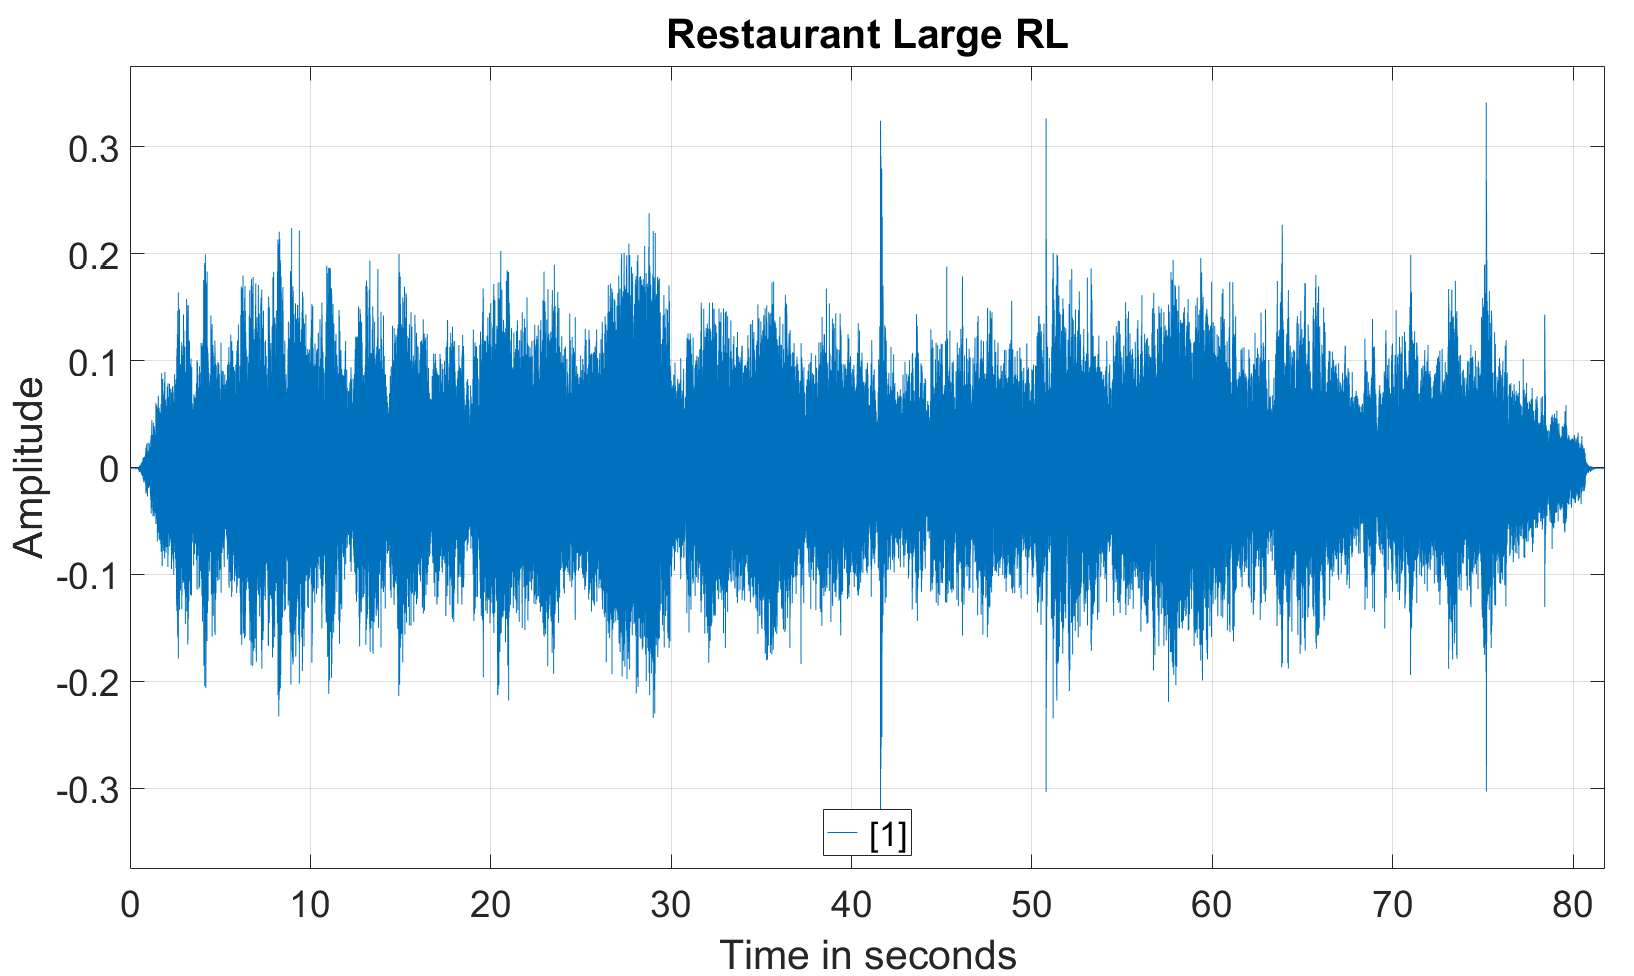
\includegraphics[width=8.5cm,]{Figs/RL_time}}\quad
\subfloat[Visualização da amplitude por frequência no tempo.]{\label{rr2}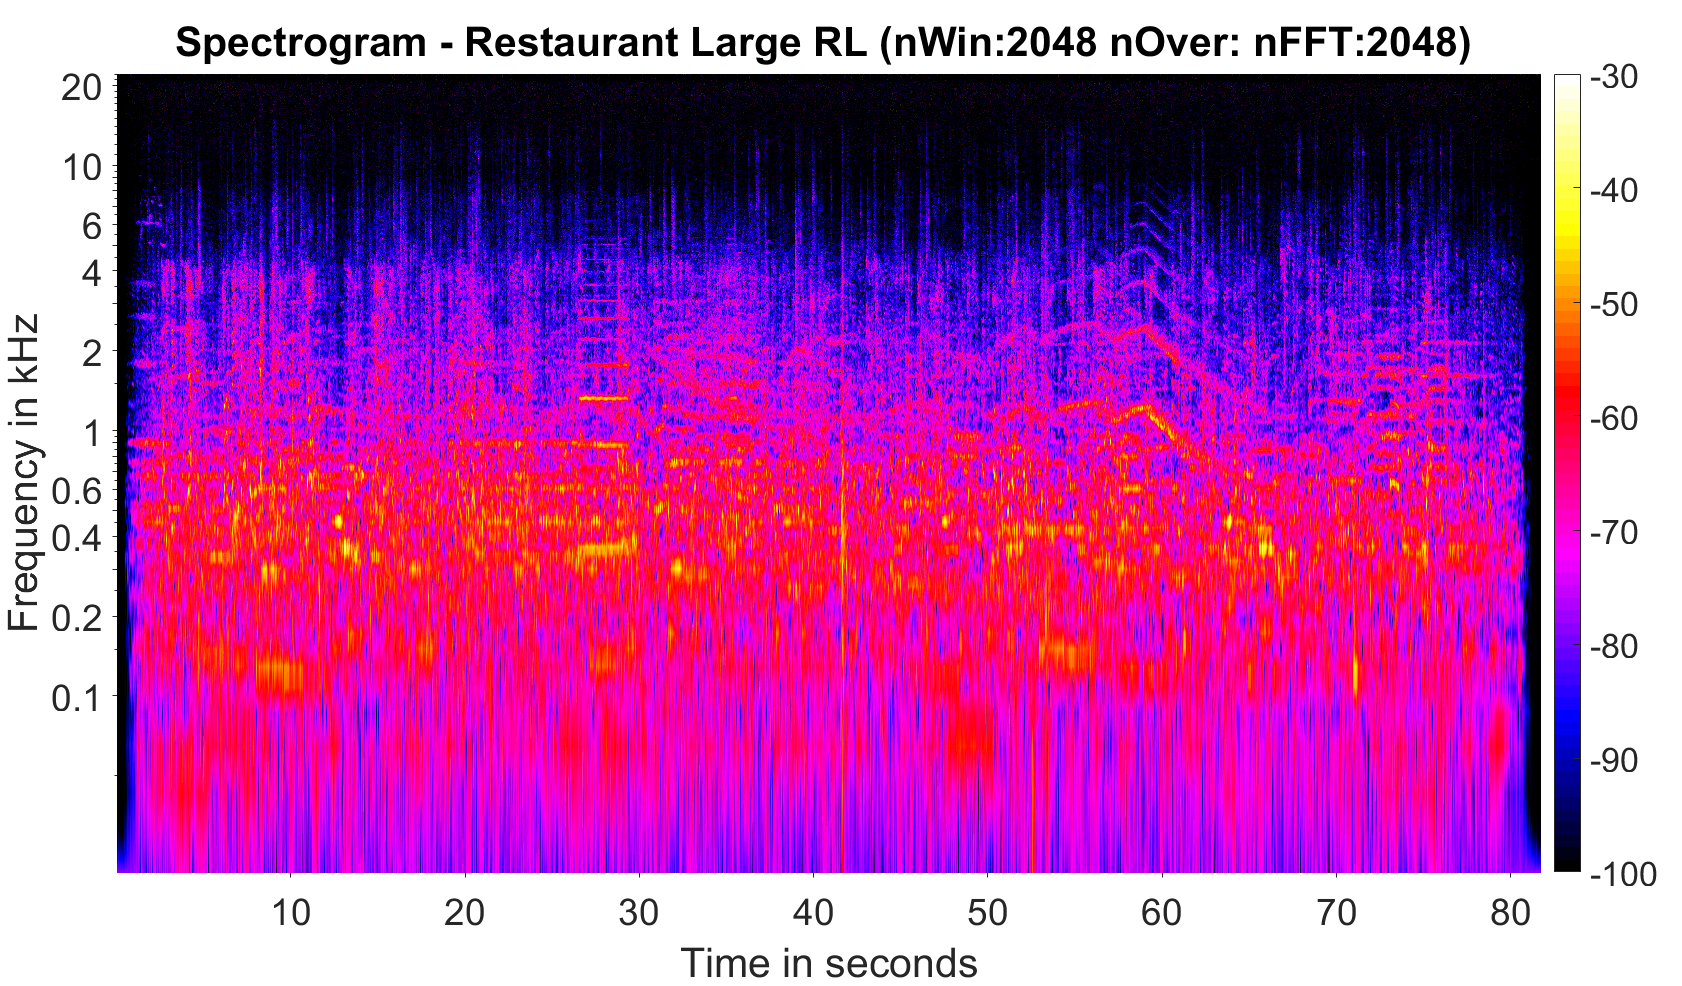
\includegraphics[width=8.5cm,]{Figs/RL_spectrograma}}
\caption{Ruído RESTAURANT\_LARGE.flac (RL).}
\label{ruidos1}
\end{figure}

As \figura{ruidos2} e \ref{ruidos3} apresentam as mesmas visualizações, para o ruído RESTAURANT\_medium.flac (RM) e RESTAURANT\_MEXICO.flac (RMX) respectivamente. 

\begin{figure}[H]
\subfloat[Visualização da amplitude no domínio do tempo .]{\label{rr3}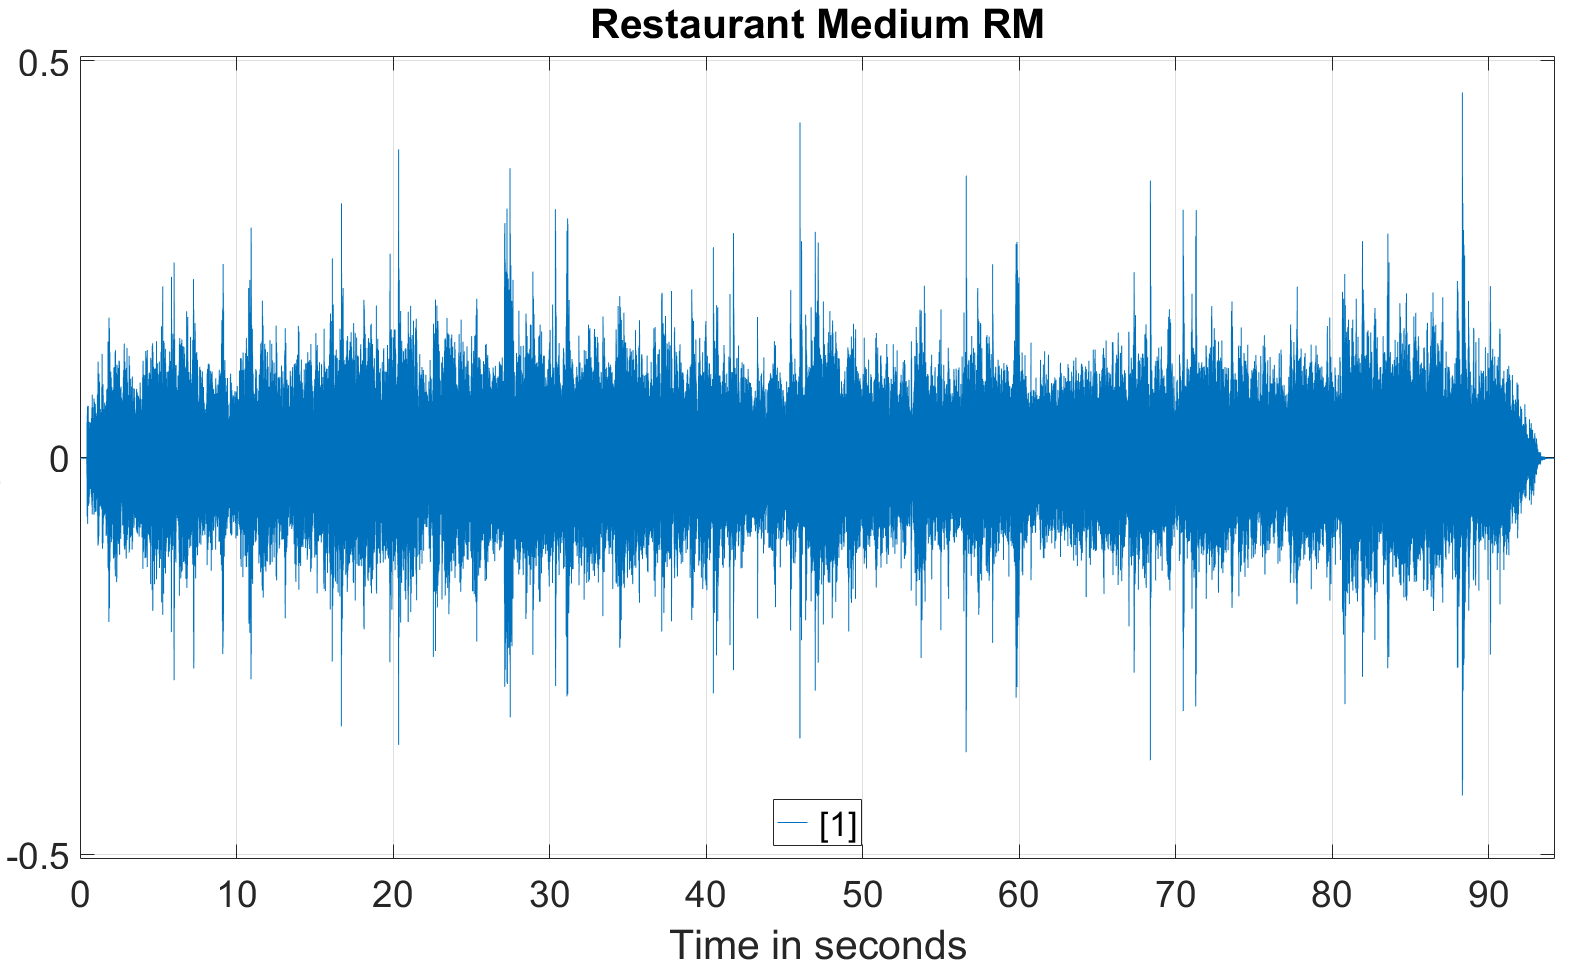
\includegraphics[width=8.5cm,]{Figs/RM_time}}\quad
\subfloat[Visualização da amplitude por frequência no tempo.]{\label{rr4}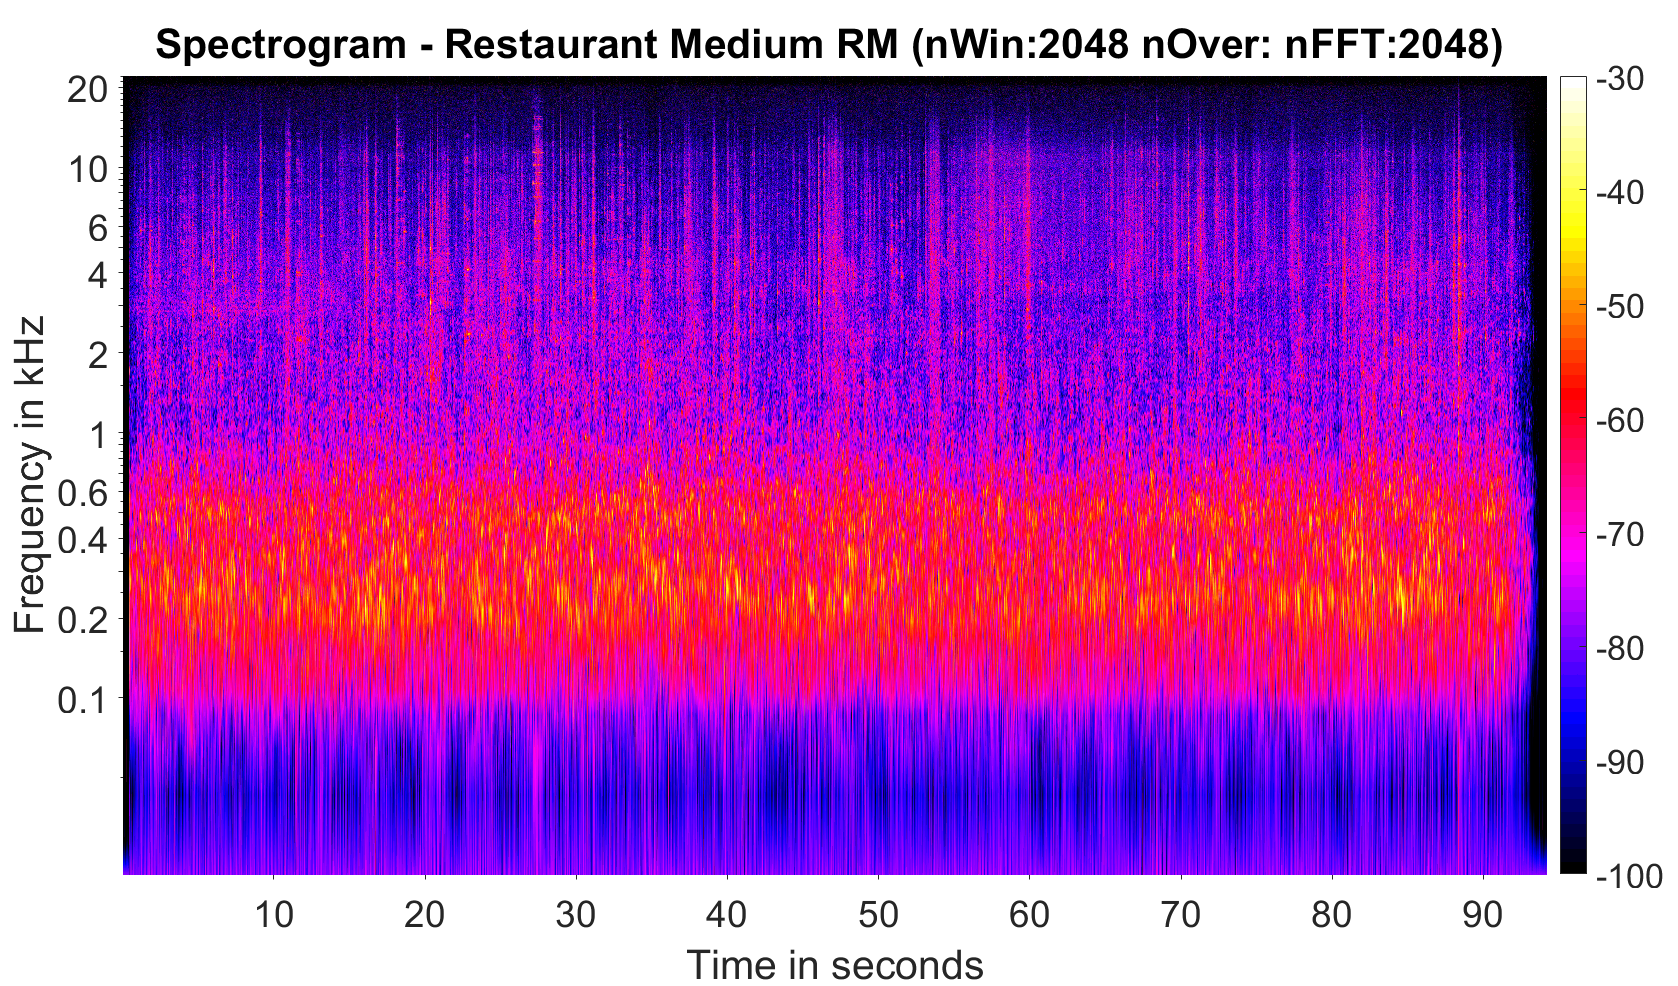
\includegraphics[width=8.5cm,]{Figs/RM_spectrograma}}
\caption{Ruído RESTAURANT\_medium.flac (RM).}
\label{ruidos2}
\end{figure}

\begin{figure}[H]
\subfloat[Visualização da amplitude no domínio do tempo .]{\label{rr5}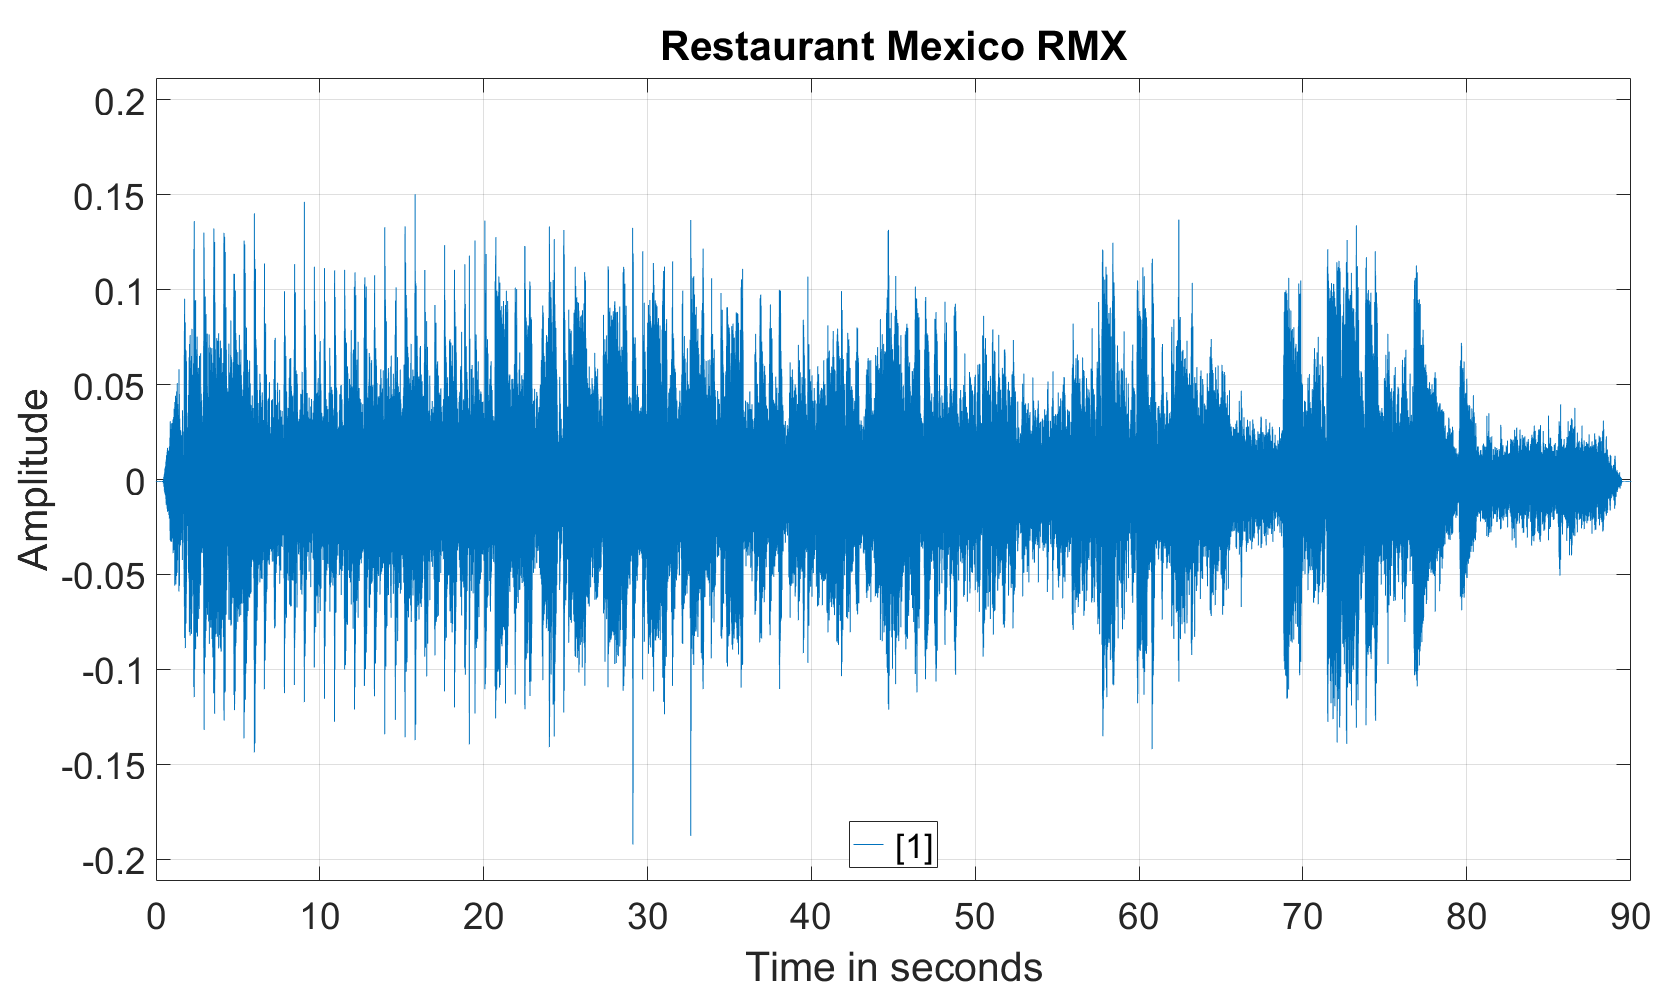
\includegraphics[width=8.5cm,]{Figs/RMX_time}}\quad
\subfloat[Visualização da amplitude por frequência no tempo.]{\label{rr6}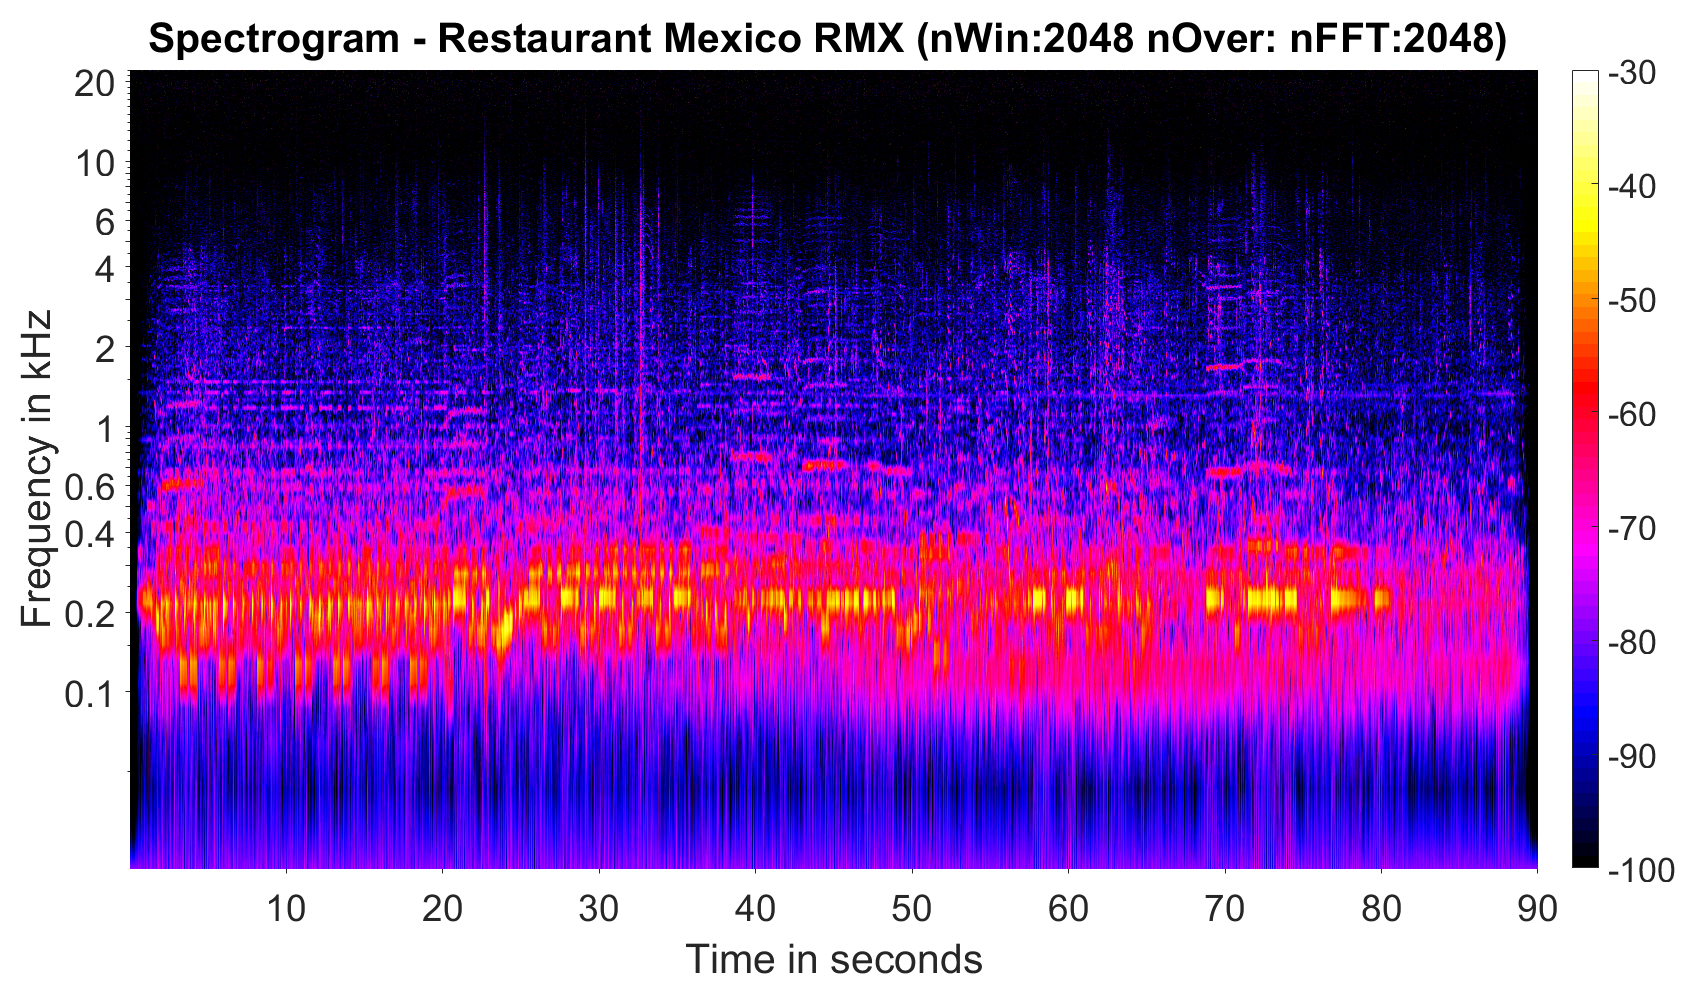
\includegraphics[width=8.5cm,]{Figs/RMX_spectrograma}}
\caption{Ruído RESTAURANT\_MEXICO.flac (RMX).}
\label{ruidos3}
\end{figure}

\subsubsection{Seleção de trecho do ruído}
Os trechos de ruído foram selecionados buscando partes do ruído que apresentassem estacionaridade, ou o mais próximo possível, para que a avaliação das técnicas estivesse garantida, contudo são ruídos compostos de bastante aleatoriedade, e características espectrais distintas com energias em faixas de frequência distintas ou intermitências associadas ao sinal e ainda tons provenientes de instrumentos musicais. Assim o ruído influência na avaliação da técnica, contudo pode-se aproximar mais da variação de situações que existem, abrangendo uma gama maior de aspectos no momento da avaliação.

A seção de 5 segundos (segundo 1 ao 6) subtraída do áudio total (RL) é apresentada no domínio do tempo na \figura{RL_tempo}, e no espectrograma apresentado na \figura{RL_spectrograma}, denominado RL1. 


\begin{figure}[H]
\subfloat[Visualização da amplitude no domínio do tempo .]{\label{RL_tempo}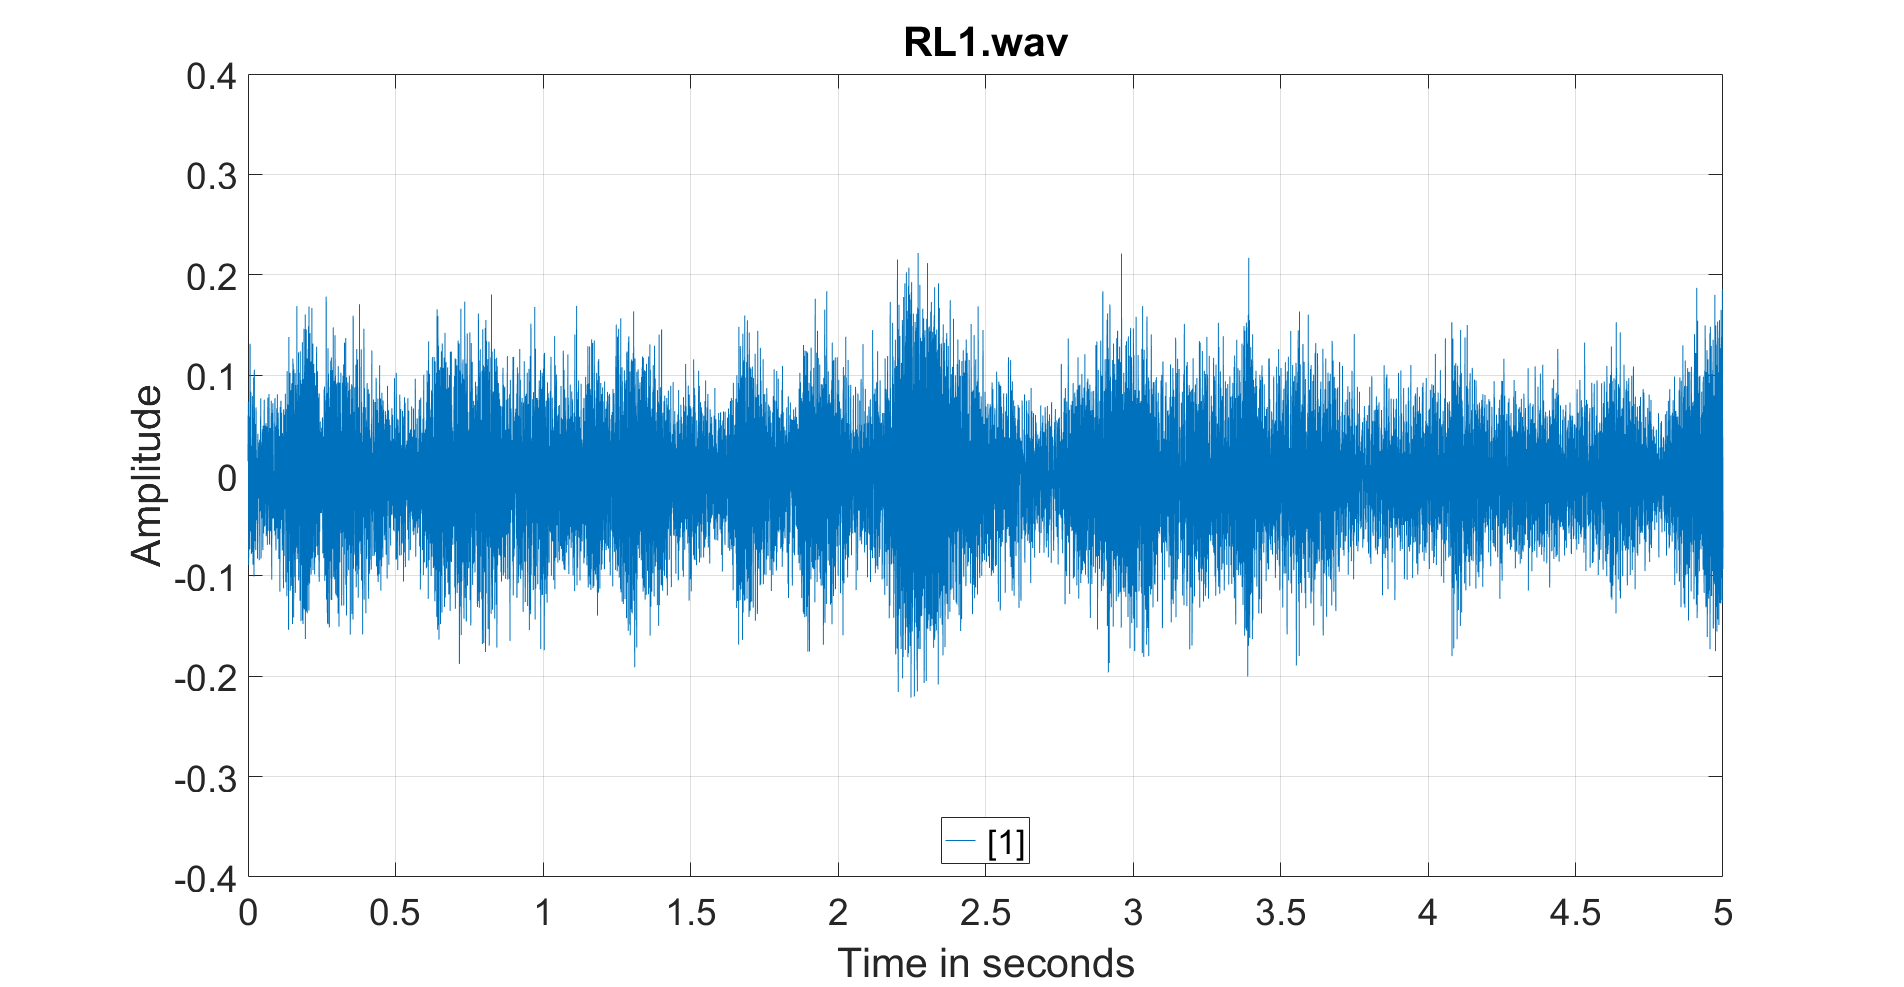
\includegraphics[width=8.5cm,]{Figs/RL1_time}}\quad
\subfloat[Visualização da amplitude por frequência no tempo.]{\label{RL_spectrograma}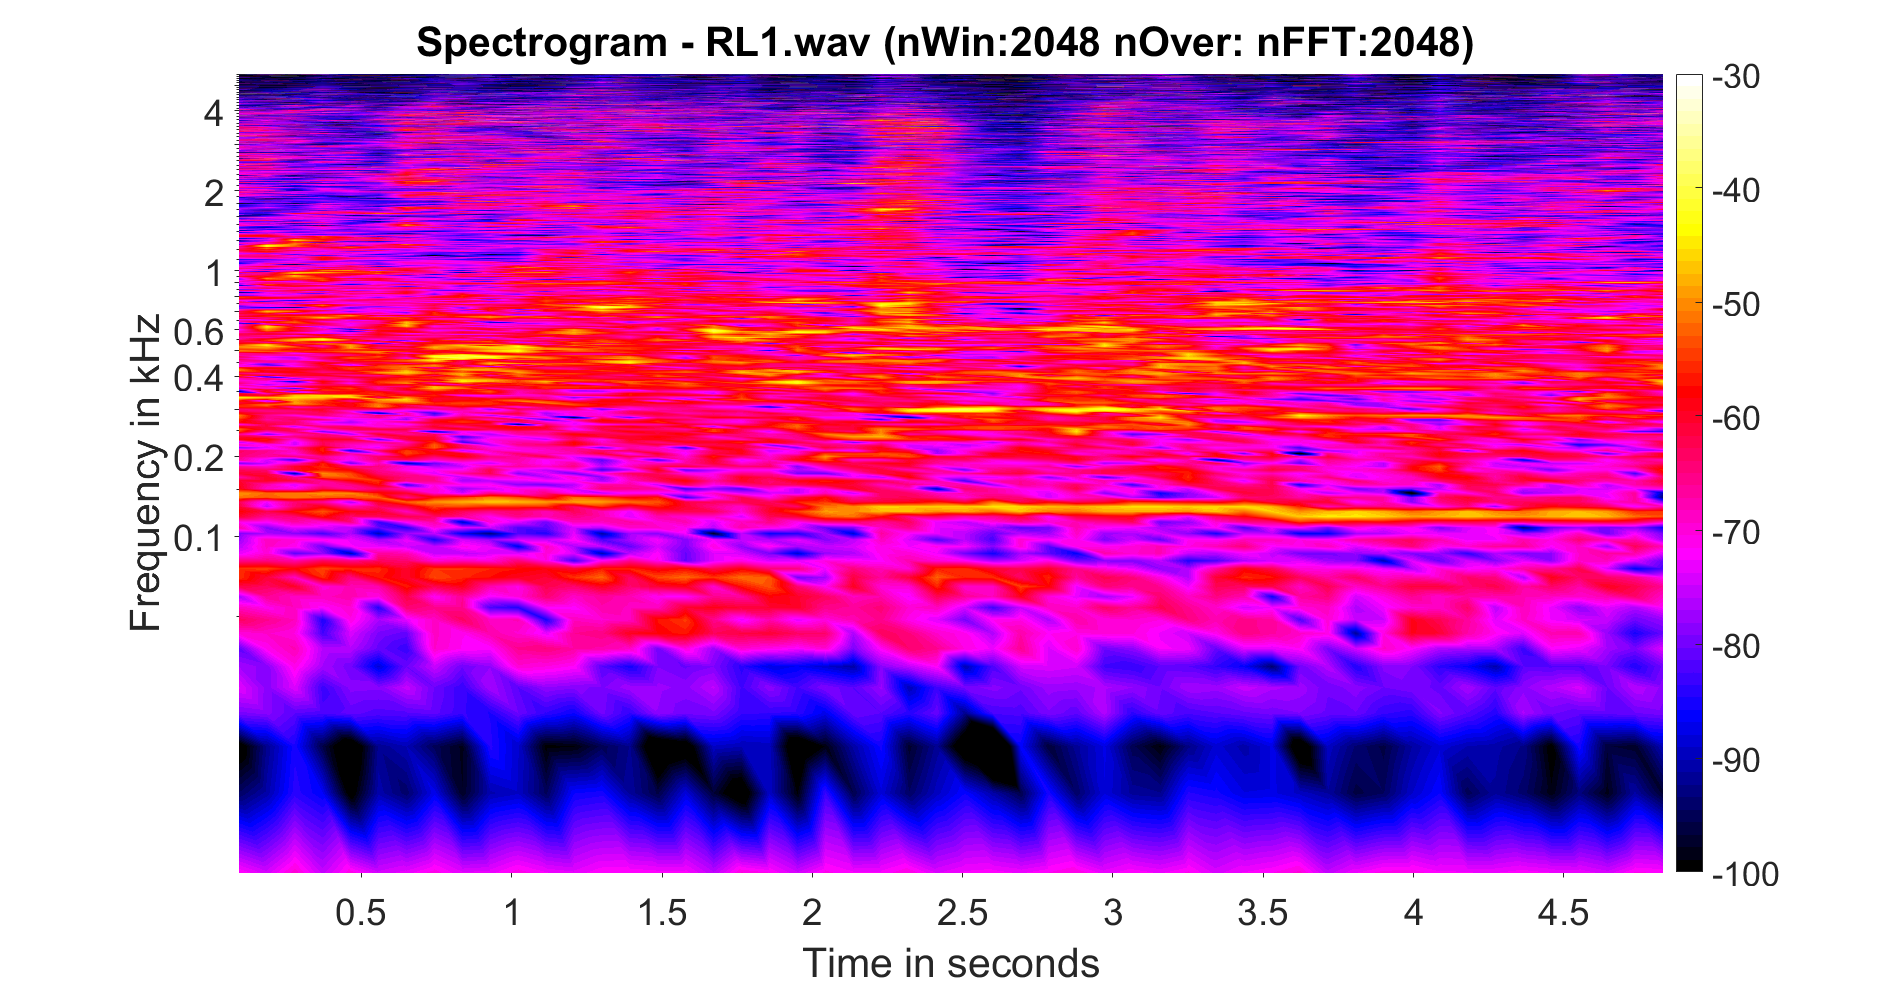
\includegraphics[width=8.5cm,]{Figs/RL1_espectrograma}}
\caption{Trecho de ruído RL.}
\label{ruidos4}
\end{figure}


A seção de 5 segundos (segundo 22 ao 27) subtraída do áudio total é apresentada no domínio do tempo na \figura{RM_tempo}, e no espectrograma apresentado na \figura{RM_spectrograma} , denominado RM1.


\begin{figure}[H]
\subfloat[Visualização da amplitude no domínio do tempo .]{\label{RM_tempo}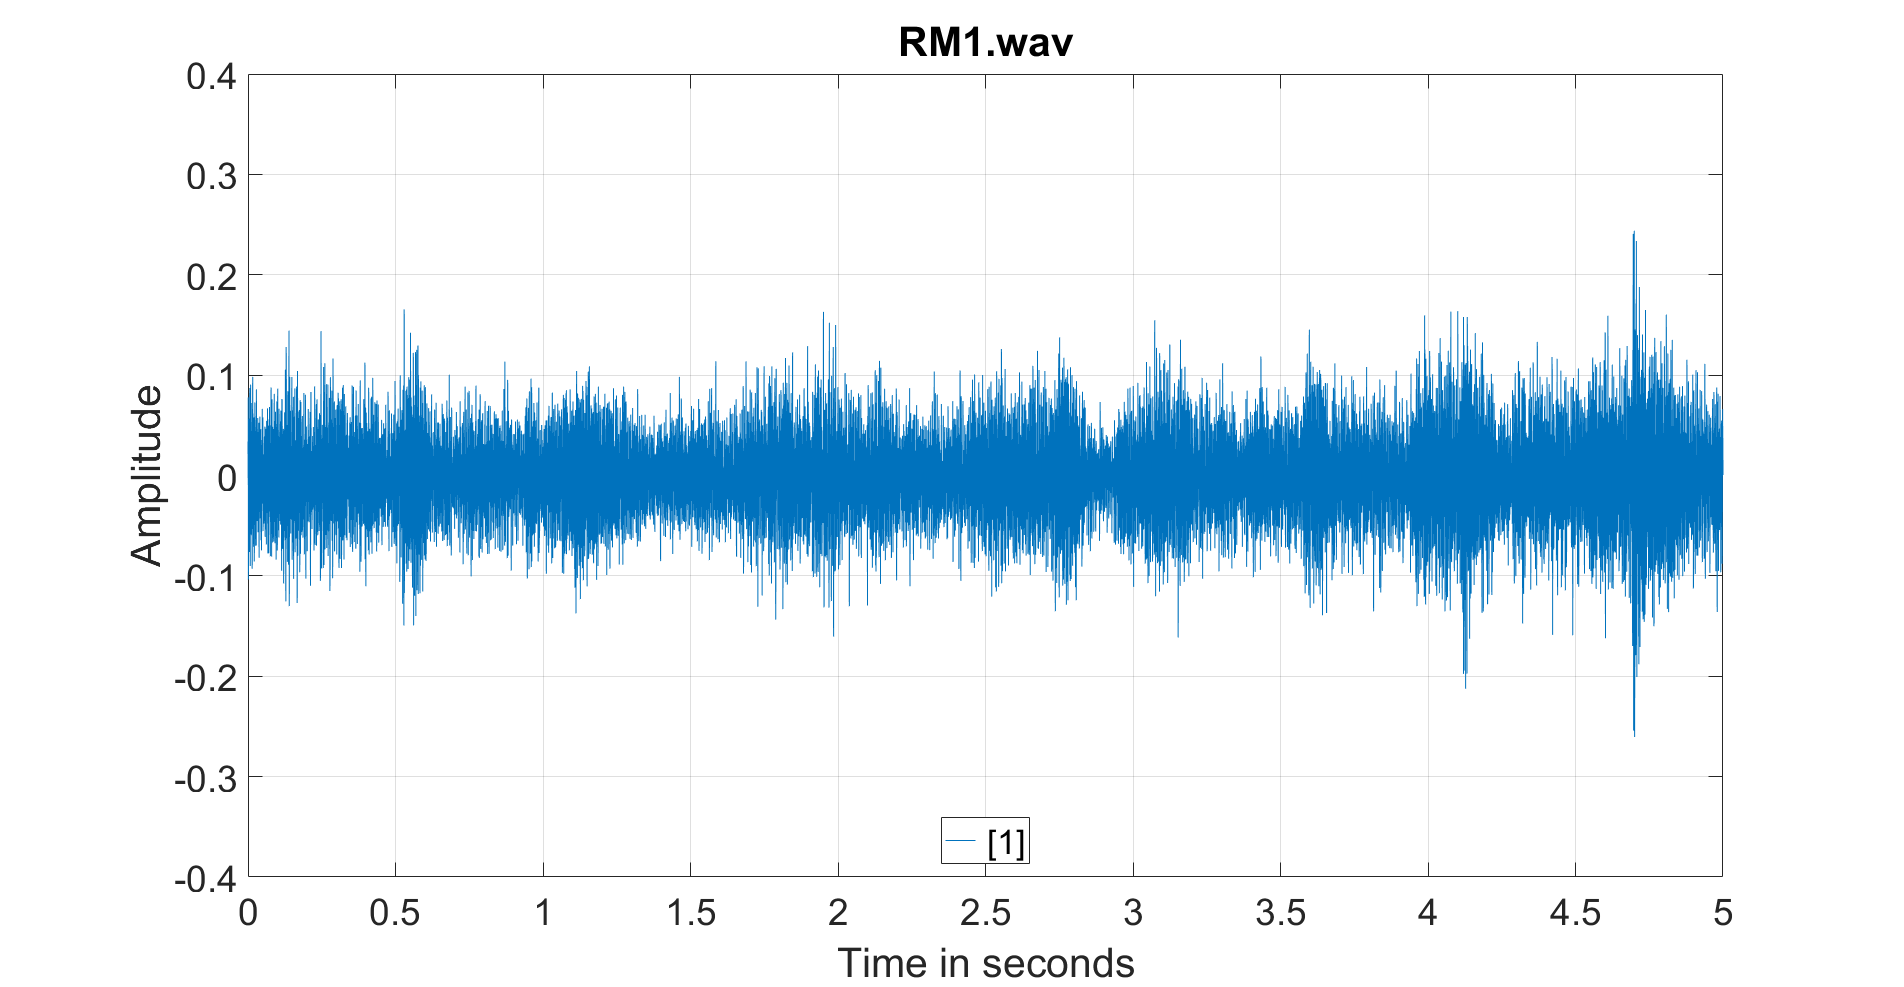
\includegraphics[width=8.5cm,]{Figs/RM1_time}}\quad
\subfloat[Visualização da amplitude por frequência no tempo.]{\label{RM_spectrograma}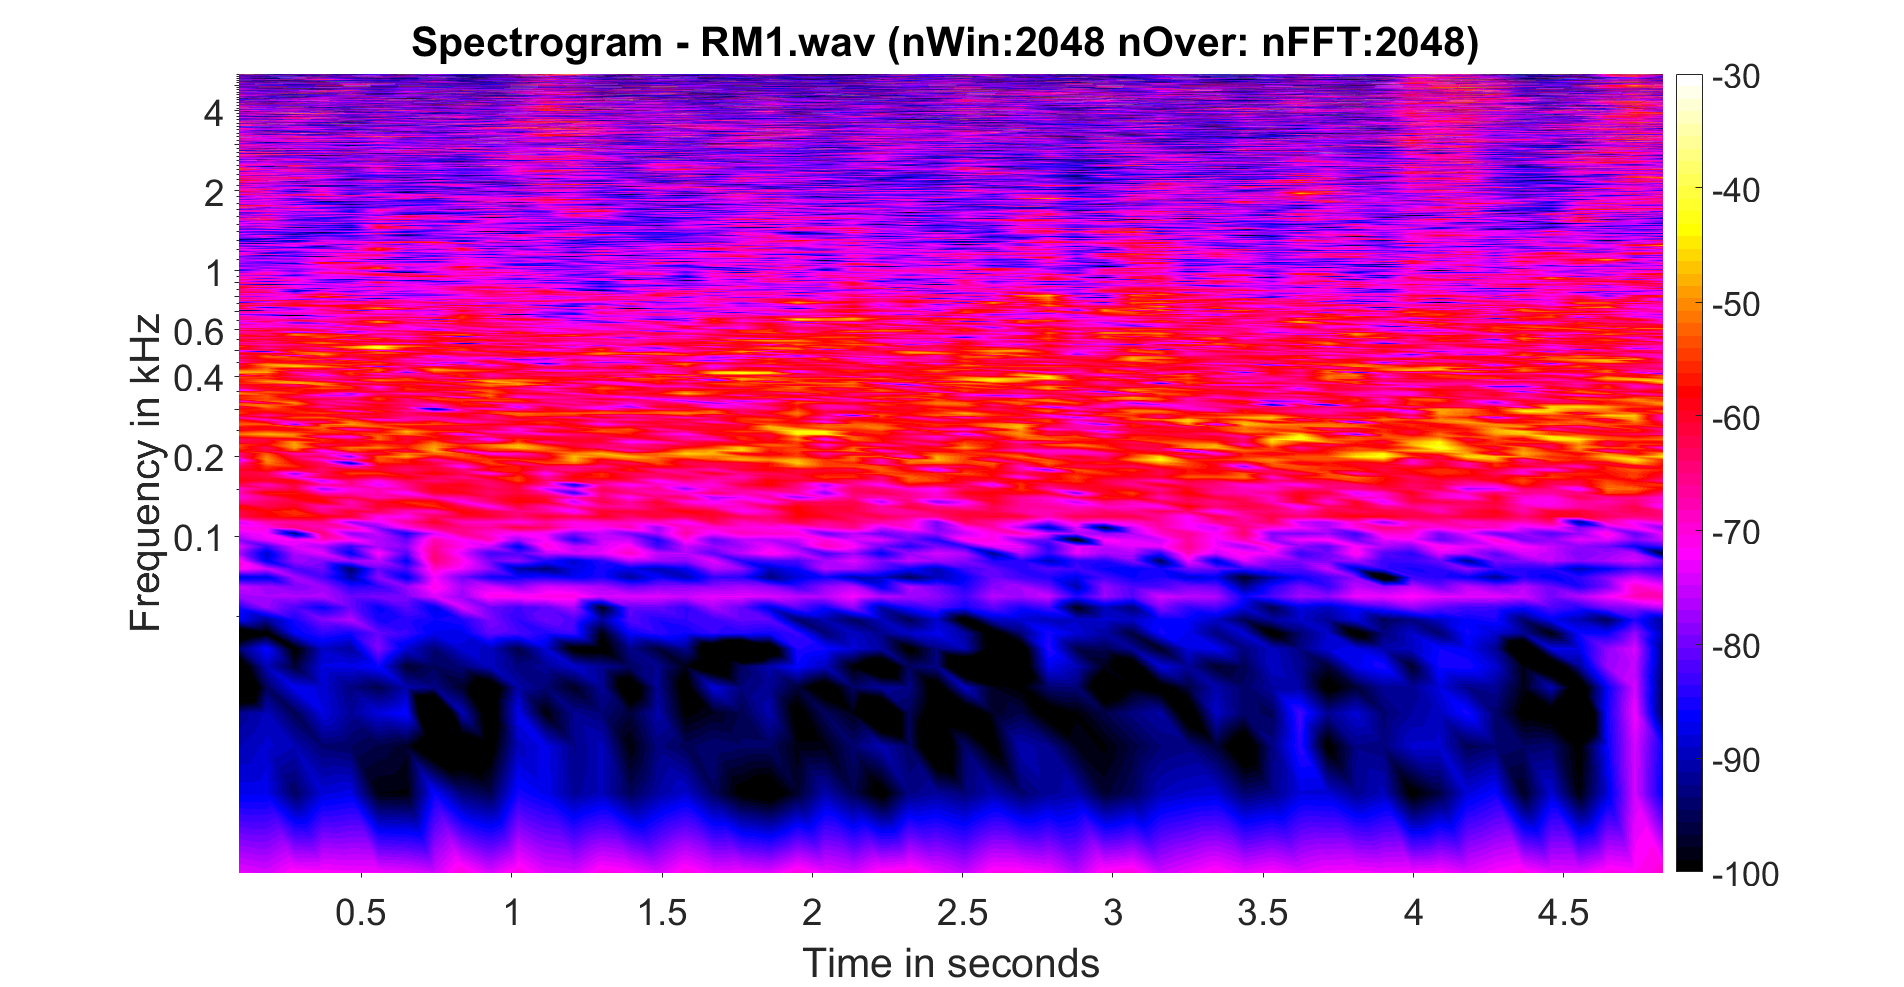
\includegraphics[width=8.5cm,]{Figs/RM1_espectrograma}}
\caption{Trecho de ruído RM.}
\label{ruidos5}
\end{figure}


A seção de 5 segundos (segundo 35 ao 40) subtraída do áudio total é apresentada no domínio do tempo na \figura{RMX_tempo}, e no espectrograma apresentado na \figura{RMX_spectrograma} , denominado RMX1.


\begin{figure}[H]
\subfloat[Visualização da amplitude no domínio do tempo .]{\label{RMX_tempo}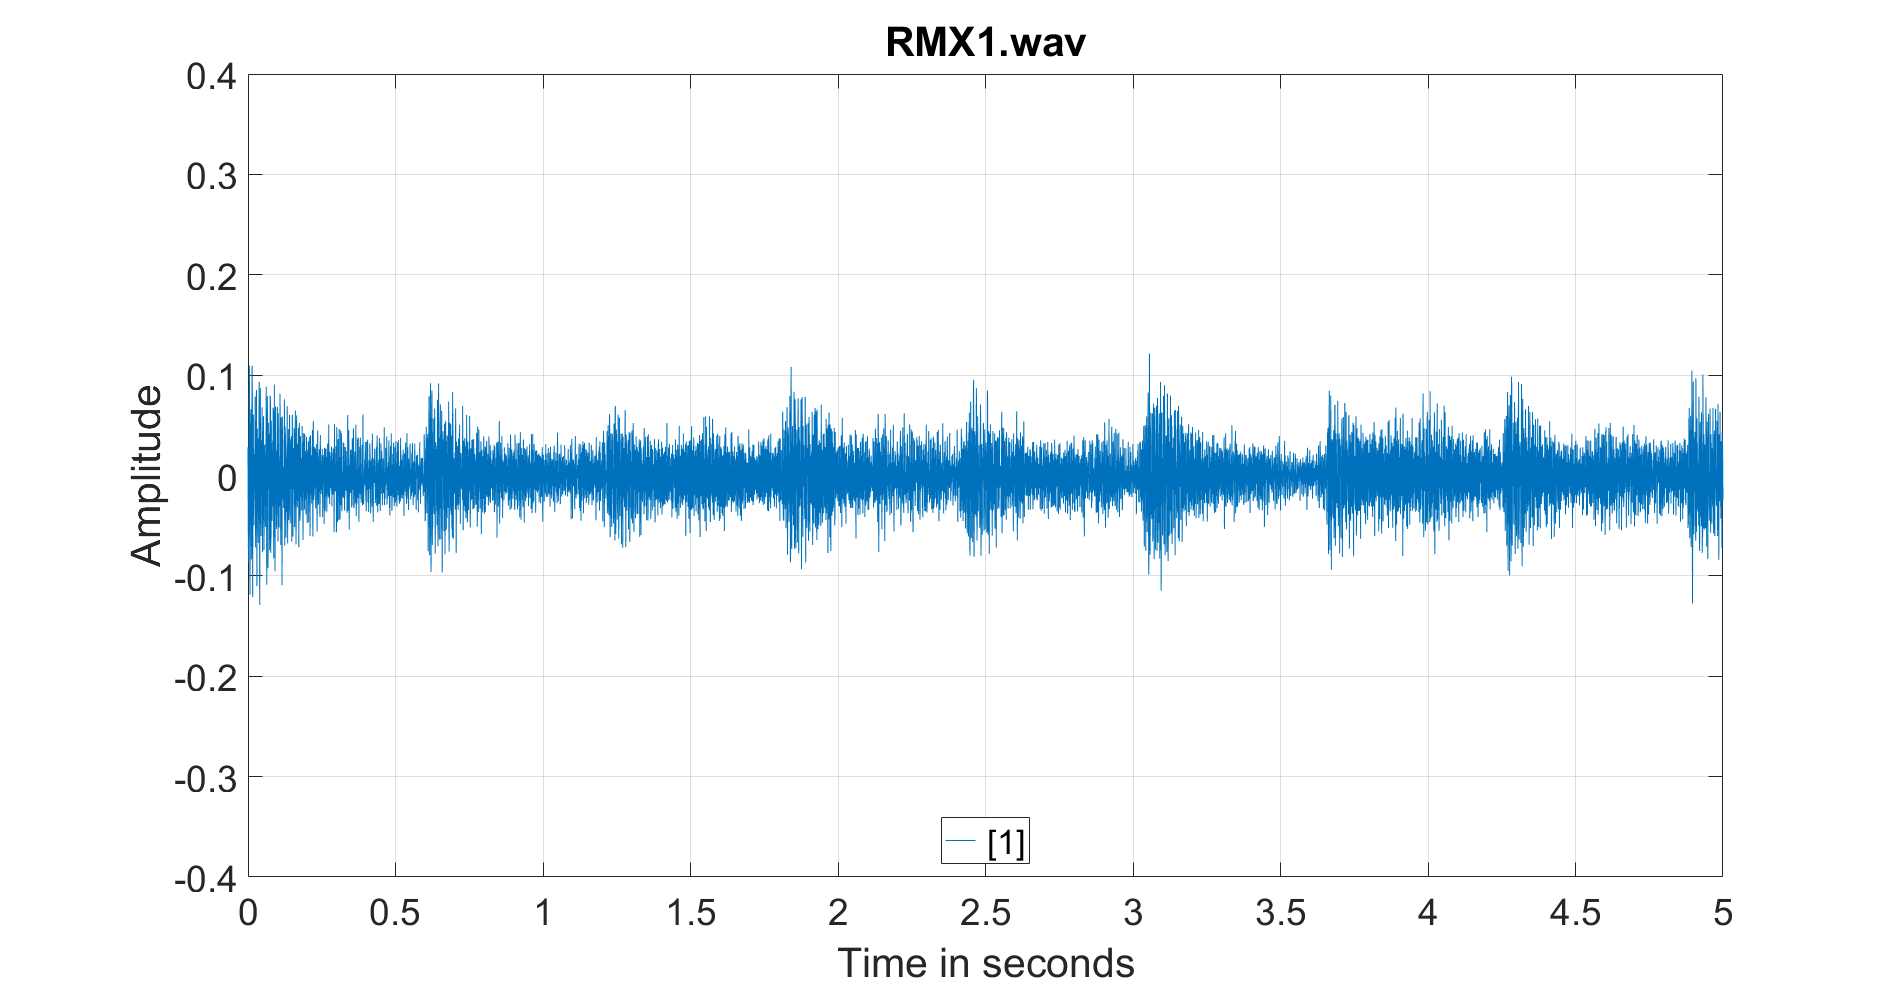
\includegraphics[width=8.5cm,]{Figs/RMX1_time}}\quad
\subfloat[Visualização da amplitude por frequência no tempo.]{\label{RMX_spectrograma}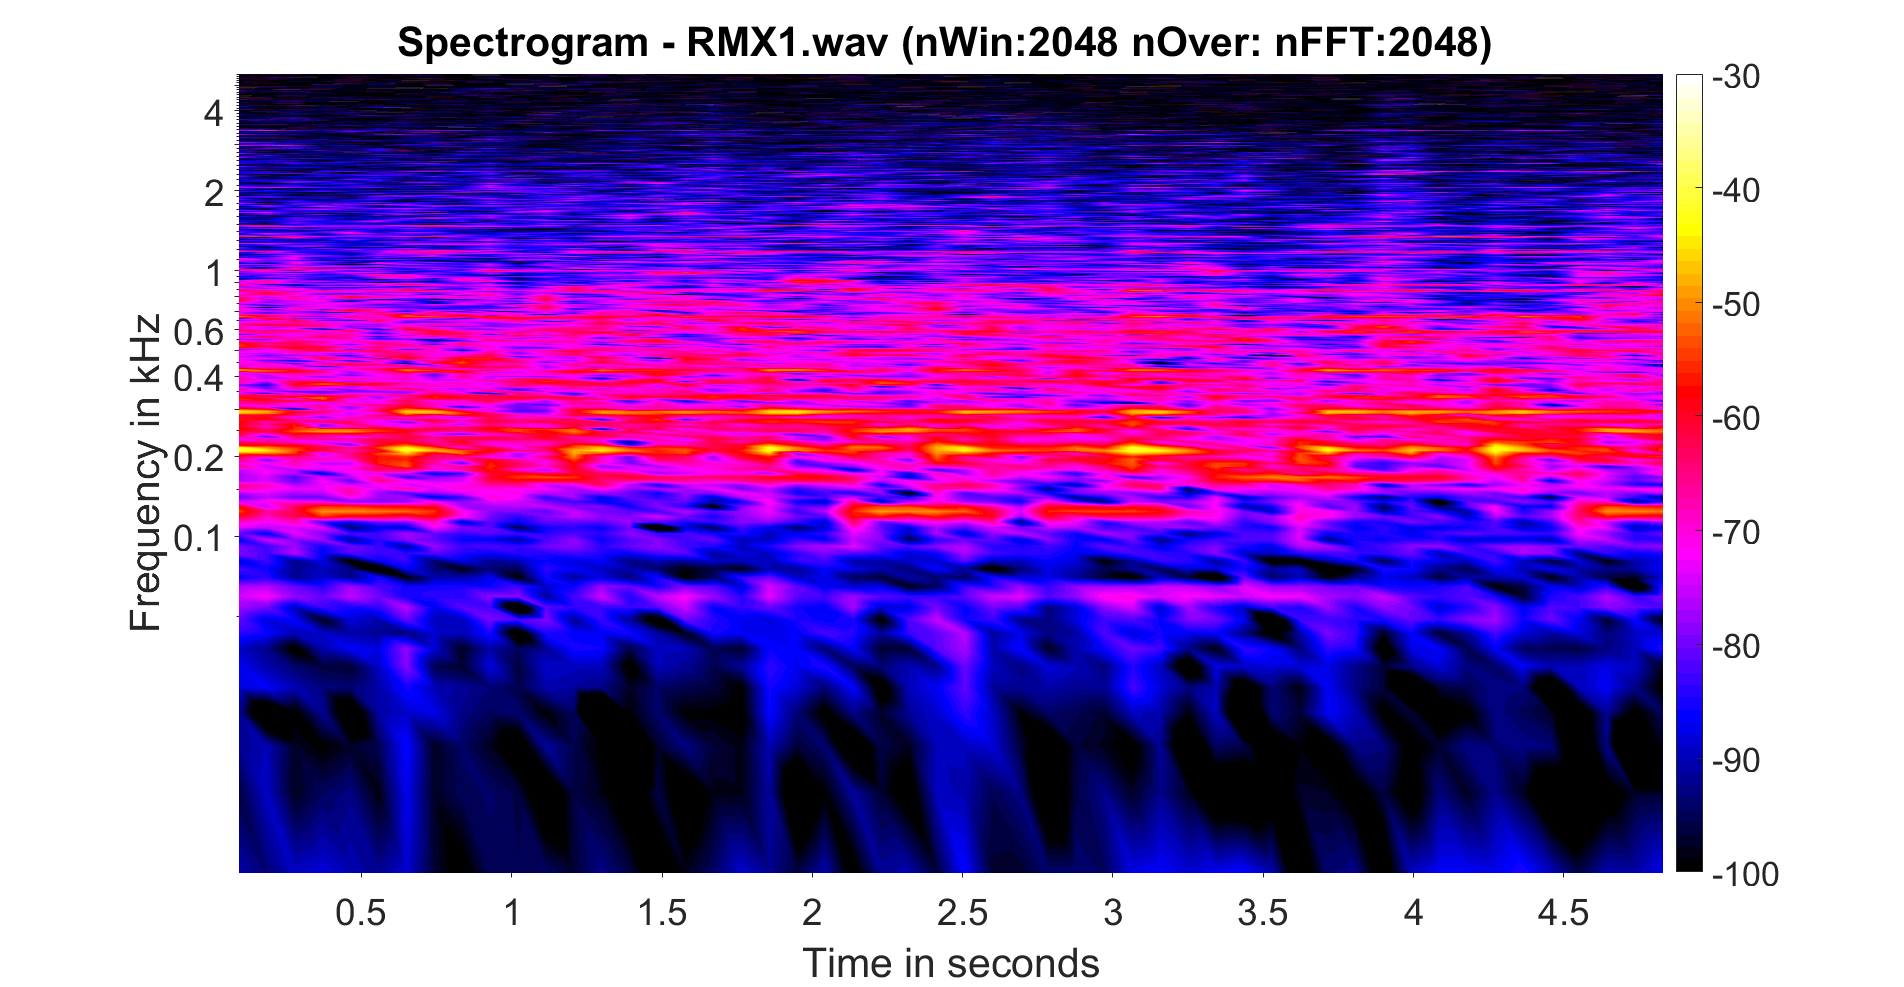
\includegraphics[width=8.5cm,]{Figs/RMX1_espectrograma}}
\caption{Trecho de ruído RM.}
\label{ruidos6}
\end{figure}






% \begin{figure}[H]
% \centering
% 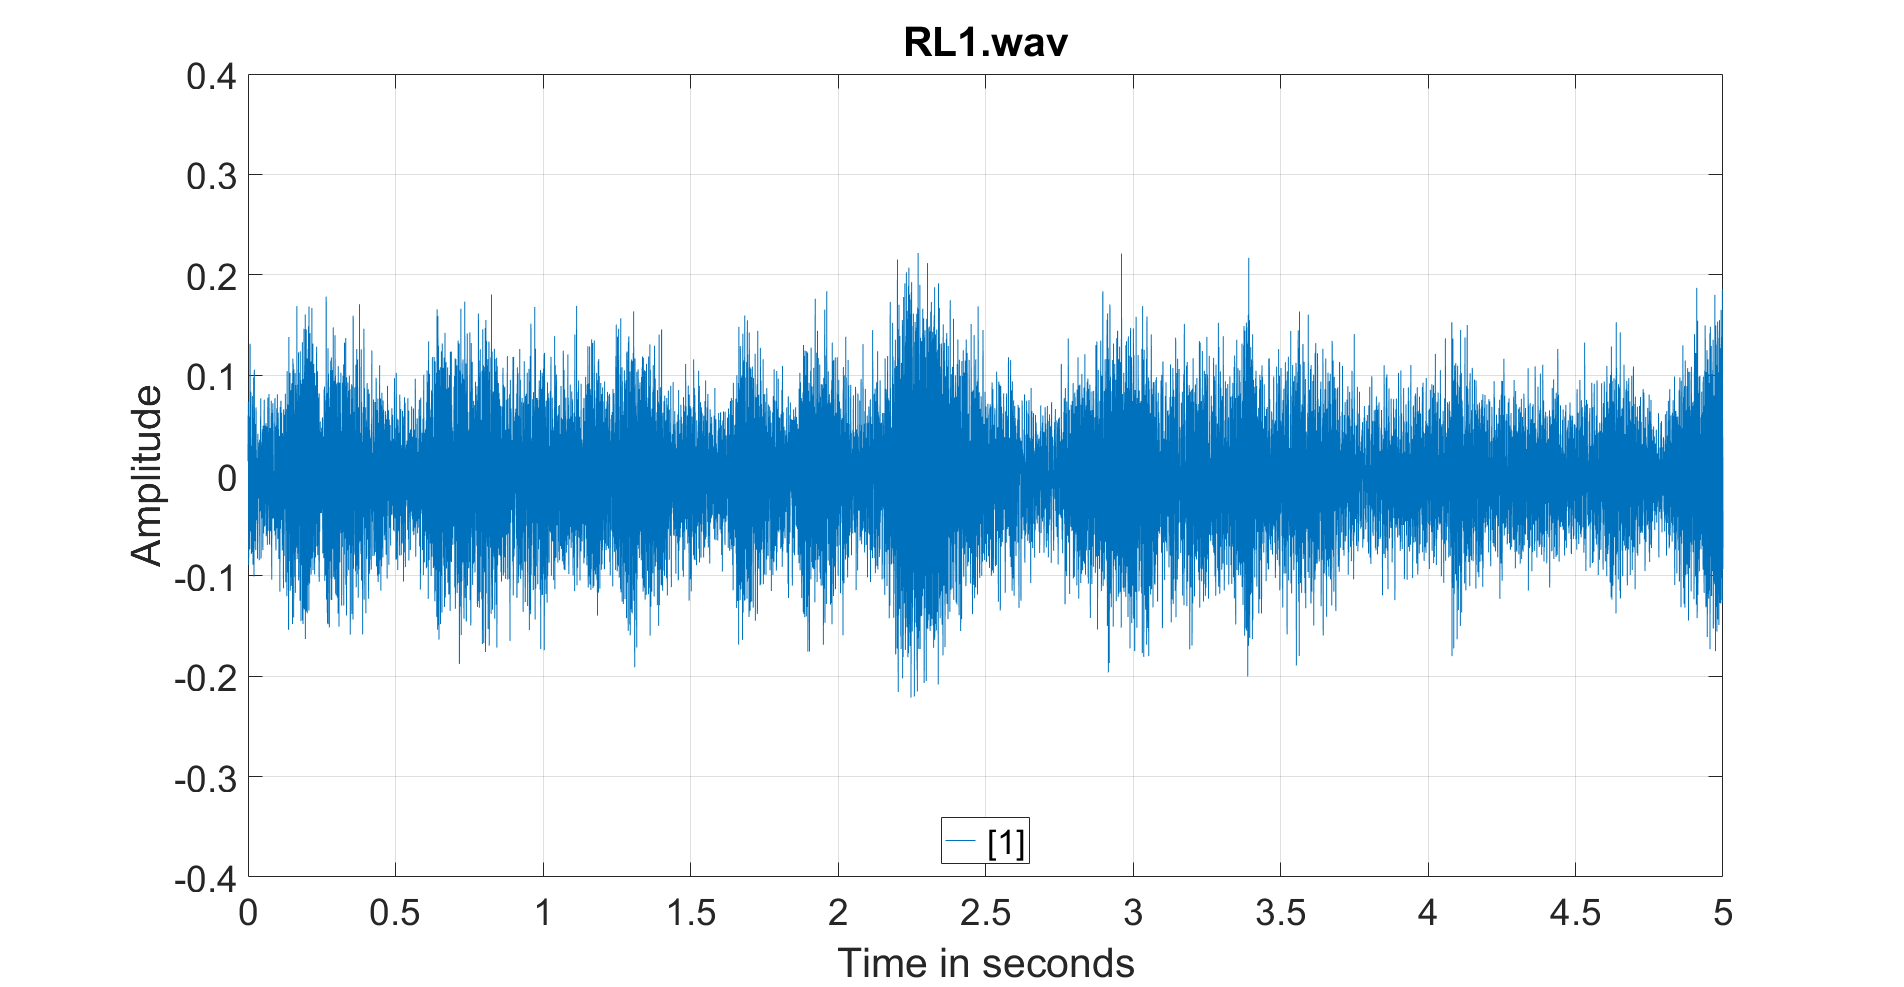
\includegraphics[width=16cm]{Figs/RL1_time.png}
% \caption{Ruído: Restaurant Large.}
% \label{RL_tempo}
% \end{figure}

% \begin{figure}[H]
% \centering
% 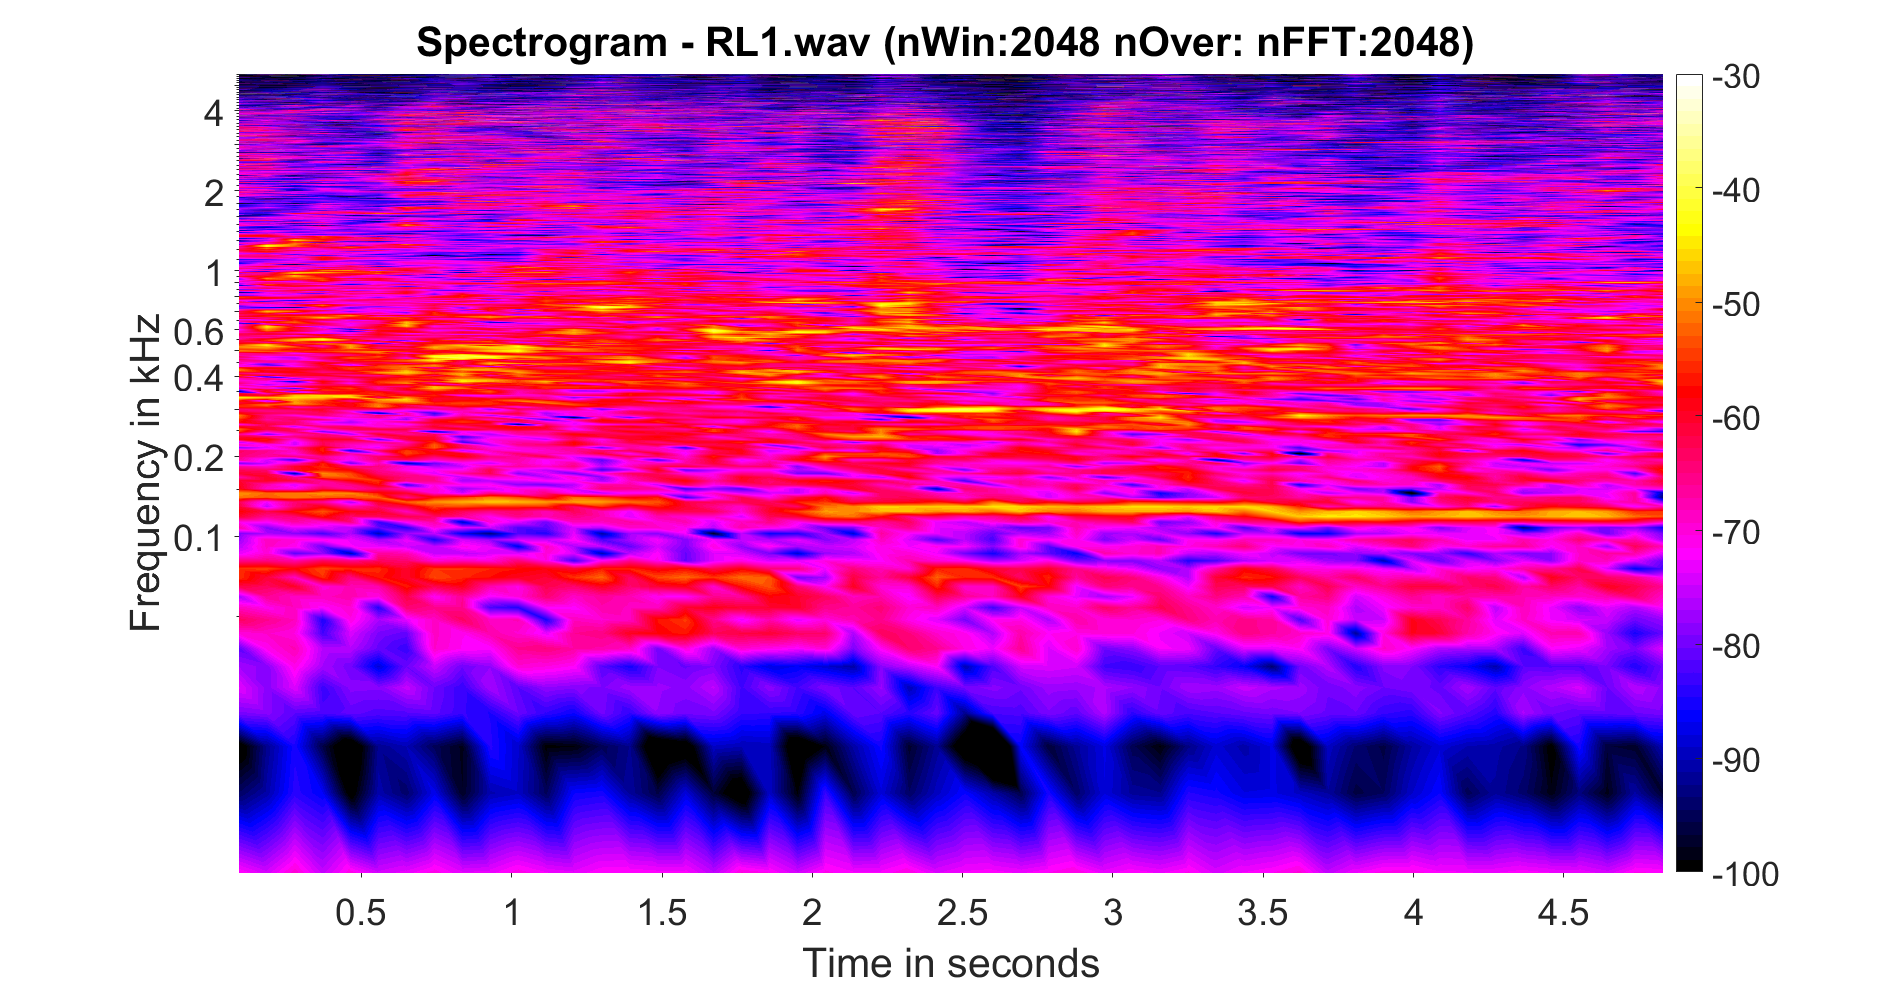
\includegraphics[width=16cm]{Figs/RL1_espectrograma.png}
% \caption{Ruído: Restaurant Large.}
% \label{RL_spectrograma}
% \end{figure}

Para o grupo total foram selecionados 5 trechos da mesma maneira de cada sinal de ruído. Os tempos selecionados foram


\section{Processamento/Análises}
O processamento dos sinais foi realizado no Matlab, onde fez-se a contaminação para cada relação sinal ruído de cada combinação de sinal de fala e sinais de ruído, aplicado os processamentos e computados os erros de entre a diferença da magnitude da resposta do sinal original e do sinal processado pela técnica (ambos na frequência) de cada \textit{bin} de frequência a cada 20 milisegundos. O somatório do erro foi normalizado pelo número de \textit{bins} a cada trecho de 20 milisegundos e posteriormente normalizado pelo número total de trechos.

Os sinais resultantes do processamento pelas técnicas foram normalizados pela máxima amplitude de cada sinal.

\subsection{Grupo de controle}

O intuito do grupo de controle é variar alguns parâmetros, apresentar as diferenças para a técnicas devido a escolha dos mesmos e definir sob algum aspecto a melhor escolha desses parâmetros a serem aplicados em um grupo maior.

Para o grupo de controle foram selecionados 10 sinais de fala, 3 SNR (-10~dB, 0~dB e 10~dB) e 3 sinais de ruído diferentes.

A métrica da avaliação objetiva a ser observada foi definida como a mediana do erro quadrático médio das apresentações de todos os ruídos combinados.


\subsubsection{Parâmetros variados}
a \figura{figParametros} apresenta um esquema das variações de parâmetros realizadas, dois parâmetros foram variados, tipo de janelamento temporal do sinal (janela Hanning, Retangular e Tukey), e um parâmetro adicional, sendo para a subtração espectral a sensibilidade do VAD, variando em 3 posições 2, 3 e 4 dB. Para a técnica de filtragem Wiener iterativo o número de iterações, variando como 2 e como 5 iterações, e o parâmetro $\alpha$ relativo a SNR a priori com valor de 0,70 e 0,98 para as técnicas Logmmse e Logmmse SPU \textit{Hard Decicion}.

\begin{figure}[H]
\centering
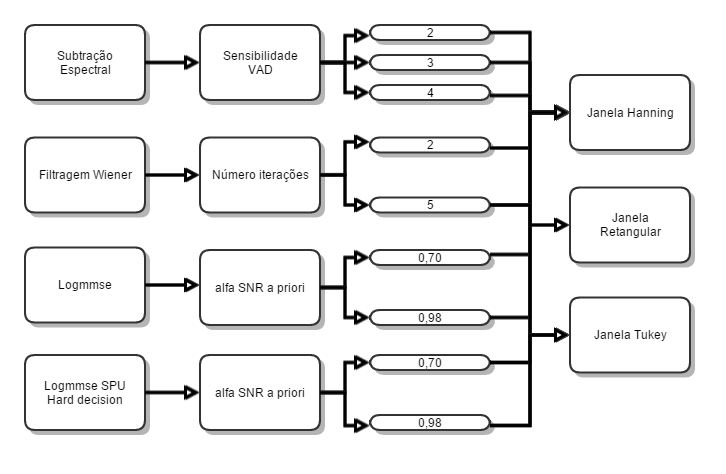
\includegraphics[width=16cm]{Figs/parametros}
\caption{Esquema de variação de parâmetros.}
\label{figParametros}
\end{figure}

Outros parâmetros poderiam ser variados para uma análise ótima, acrescentando tempo de processamento e custo computacional à analise, contudo como intuito do trabalho é o amadurecimento para o uso das técnicas e a instrumentação das mesmas, optou-se por essas variações no âmbito de demostração de influência.


\subsection{Resultados objetivos Grupo de controle}
Nesta seção serão apresentados e discutidos alguns resultados obtidos no grupo de controle variando as técnicas de processamento, os parâmetros de entrada, relações sinais ruído e sinais de fala.

\subsubsection{Análise da eficiência das técnicas em para (SNR)~-10~dB}


A \figura{m10_1} apresenta o boxplot da média do somatório dos erros quadráticos da diferença entre o sinal processado pelas técnicas escolhidas, com a variação dos parâmetros mencionados, para a relação sinal ruído de -10 dB e com o ruído contaminante RL.

\begin{figure}[H]
\centering
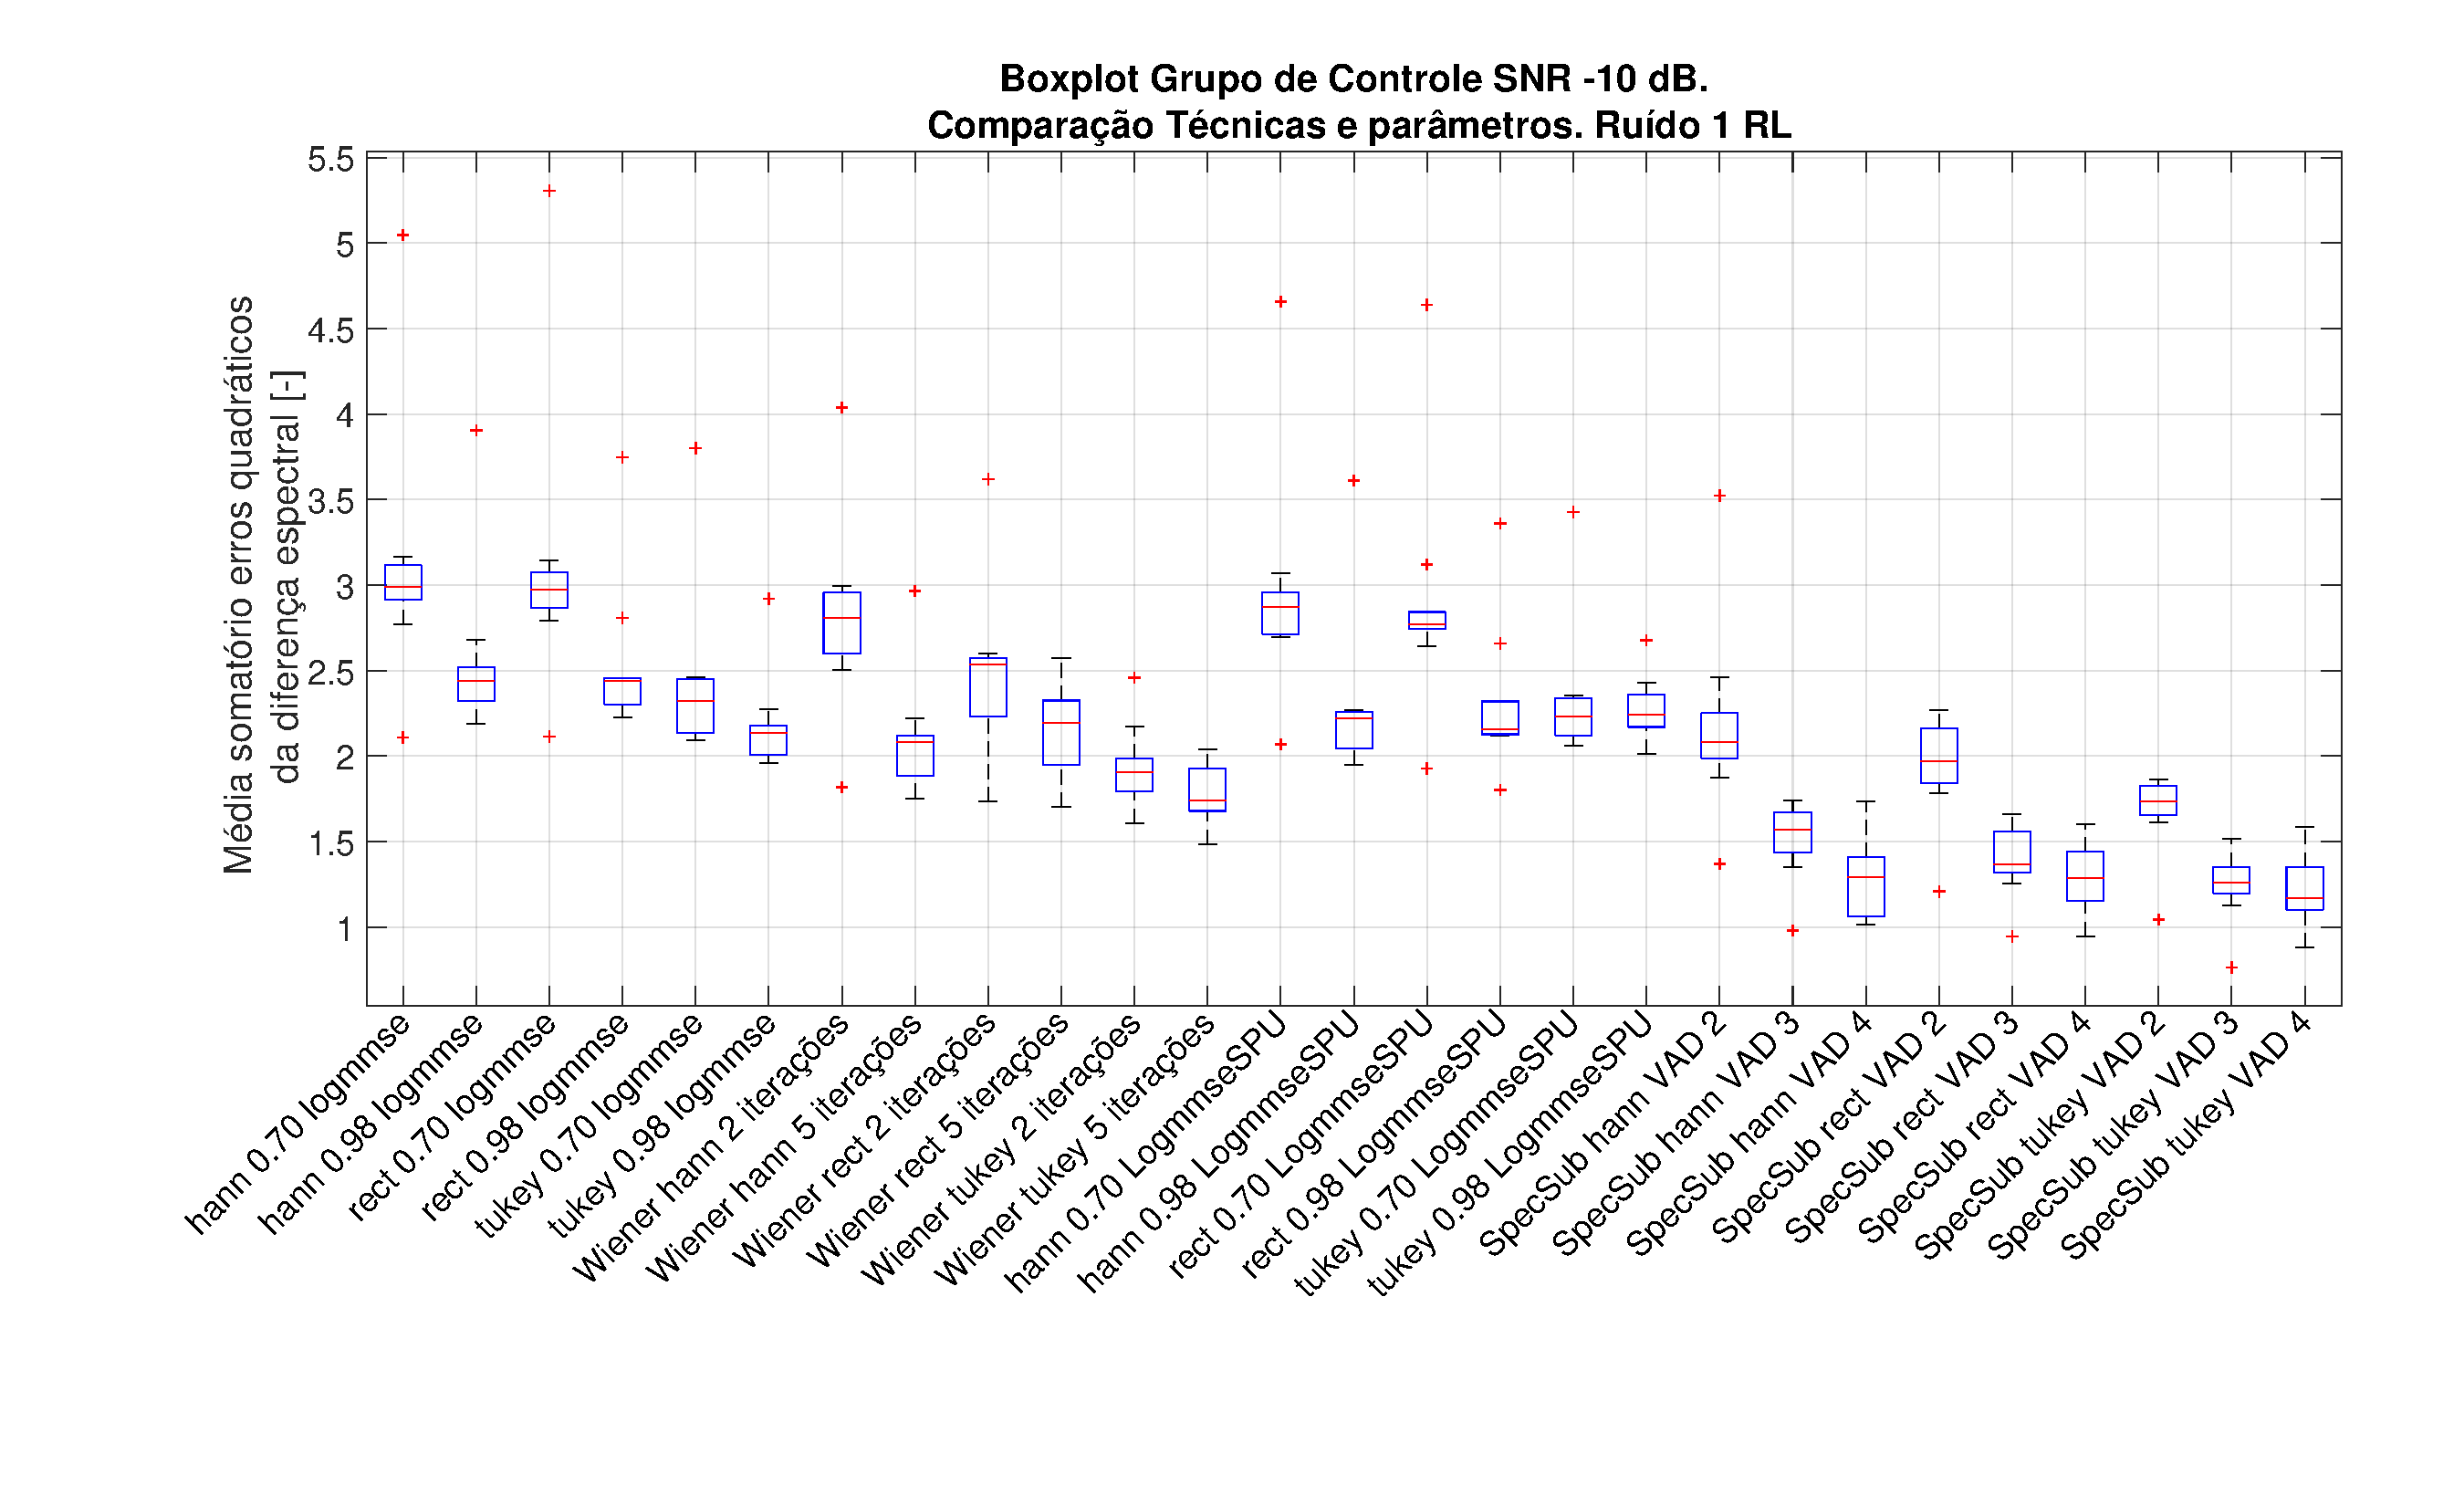
\includegraphics[width=16cm]{Figs/Erro_m10_Ruido1.pdf}
\caption{SNR -10 dB Ruído: Restaurant Large.}
\label{m10_1}
\end{figure}

A pequena relação sinal ruído apresenta um comportamento no gráfico de \textit{boxplot} com vários \textit{outliers}, apesar de mostrar uma tendência da técnica de subtração espectral (SpecSub) apresentar melhores resultados, isso não é repetido nas \figuras{m10_2} e \ref{m10_3}, que apresentam as mesmas variáveis, contudo para o ruído contaminante RM e RMX respectivamente. Na \figuras{m10_2} tem-se um espalhamento menos contudo a técnica que tem melhor resultado, tomando em conta a métrica da mediana do erro, é a Logmmse SPU e na \figuras{m10_3} a técnica de Wiener tem melhores resultados. 

Assim é inconclusivo a mensuração de qualidade da técnica a partir da soma dos erros quadráticos da diferença espectral. Dado que o resultado, além de ter sido elaborado sobre um grupo relativamente pequeno de amostras (sinais e ruídos), é bastante influenciado pelas características espectrais e variação dinâmica do ruído contaminante. 

Como análise ainda, o incremento em dB na sensibilidade do VAD na técnica de subtração espectral reduz o erro, esse comportamento é apresentado para todos ruídos.

\begin{figure}[H]
\centering
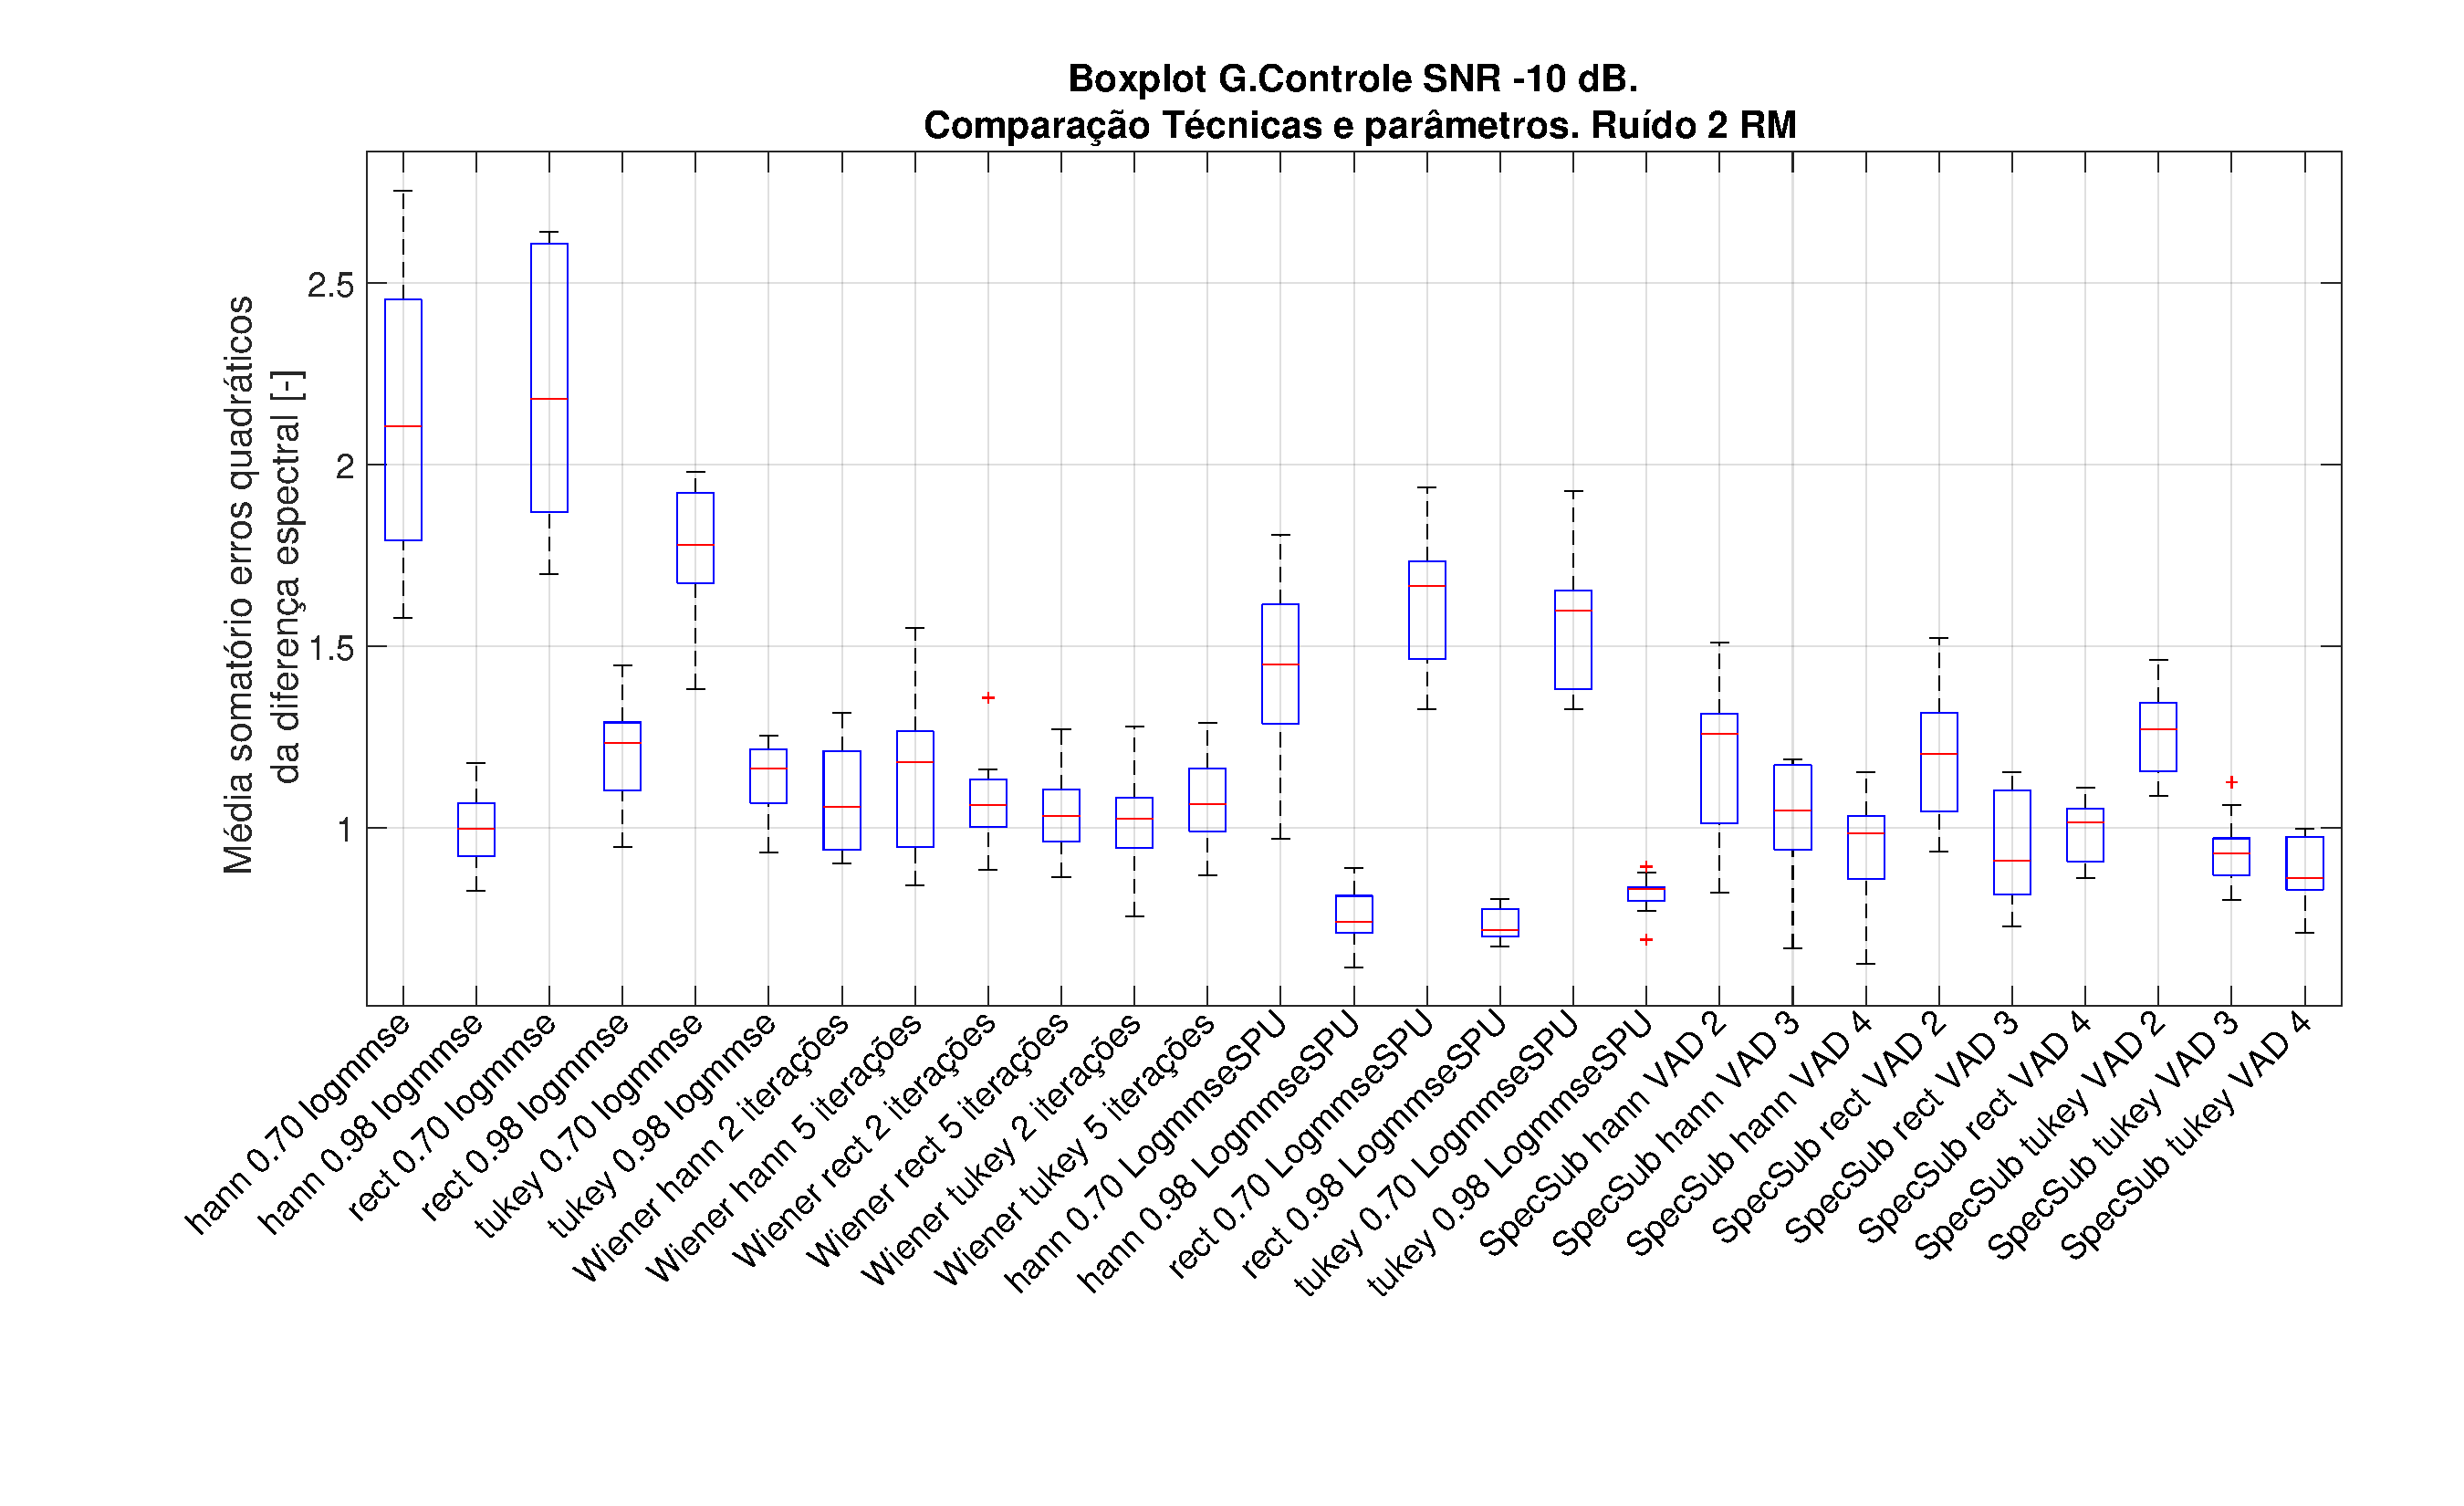
\includegraphics[width=16cm]{Figs/Erro_m10_Ruido2.pdf}
\caption{SNR -10 dB Ruído: Restaurant medium.}
\label{m10_2}
\end{figure}

\begin{figure}[H]
\centering
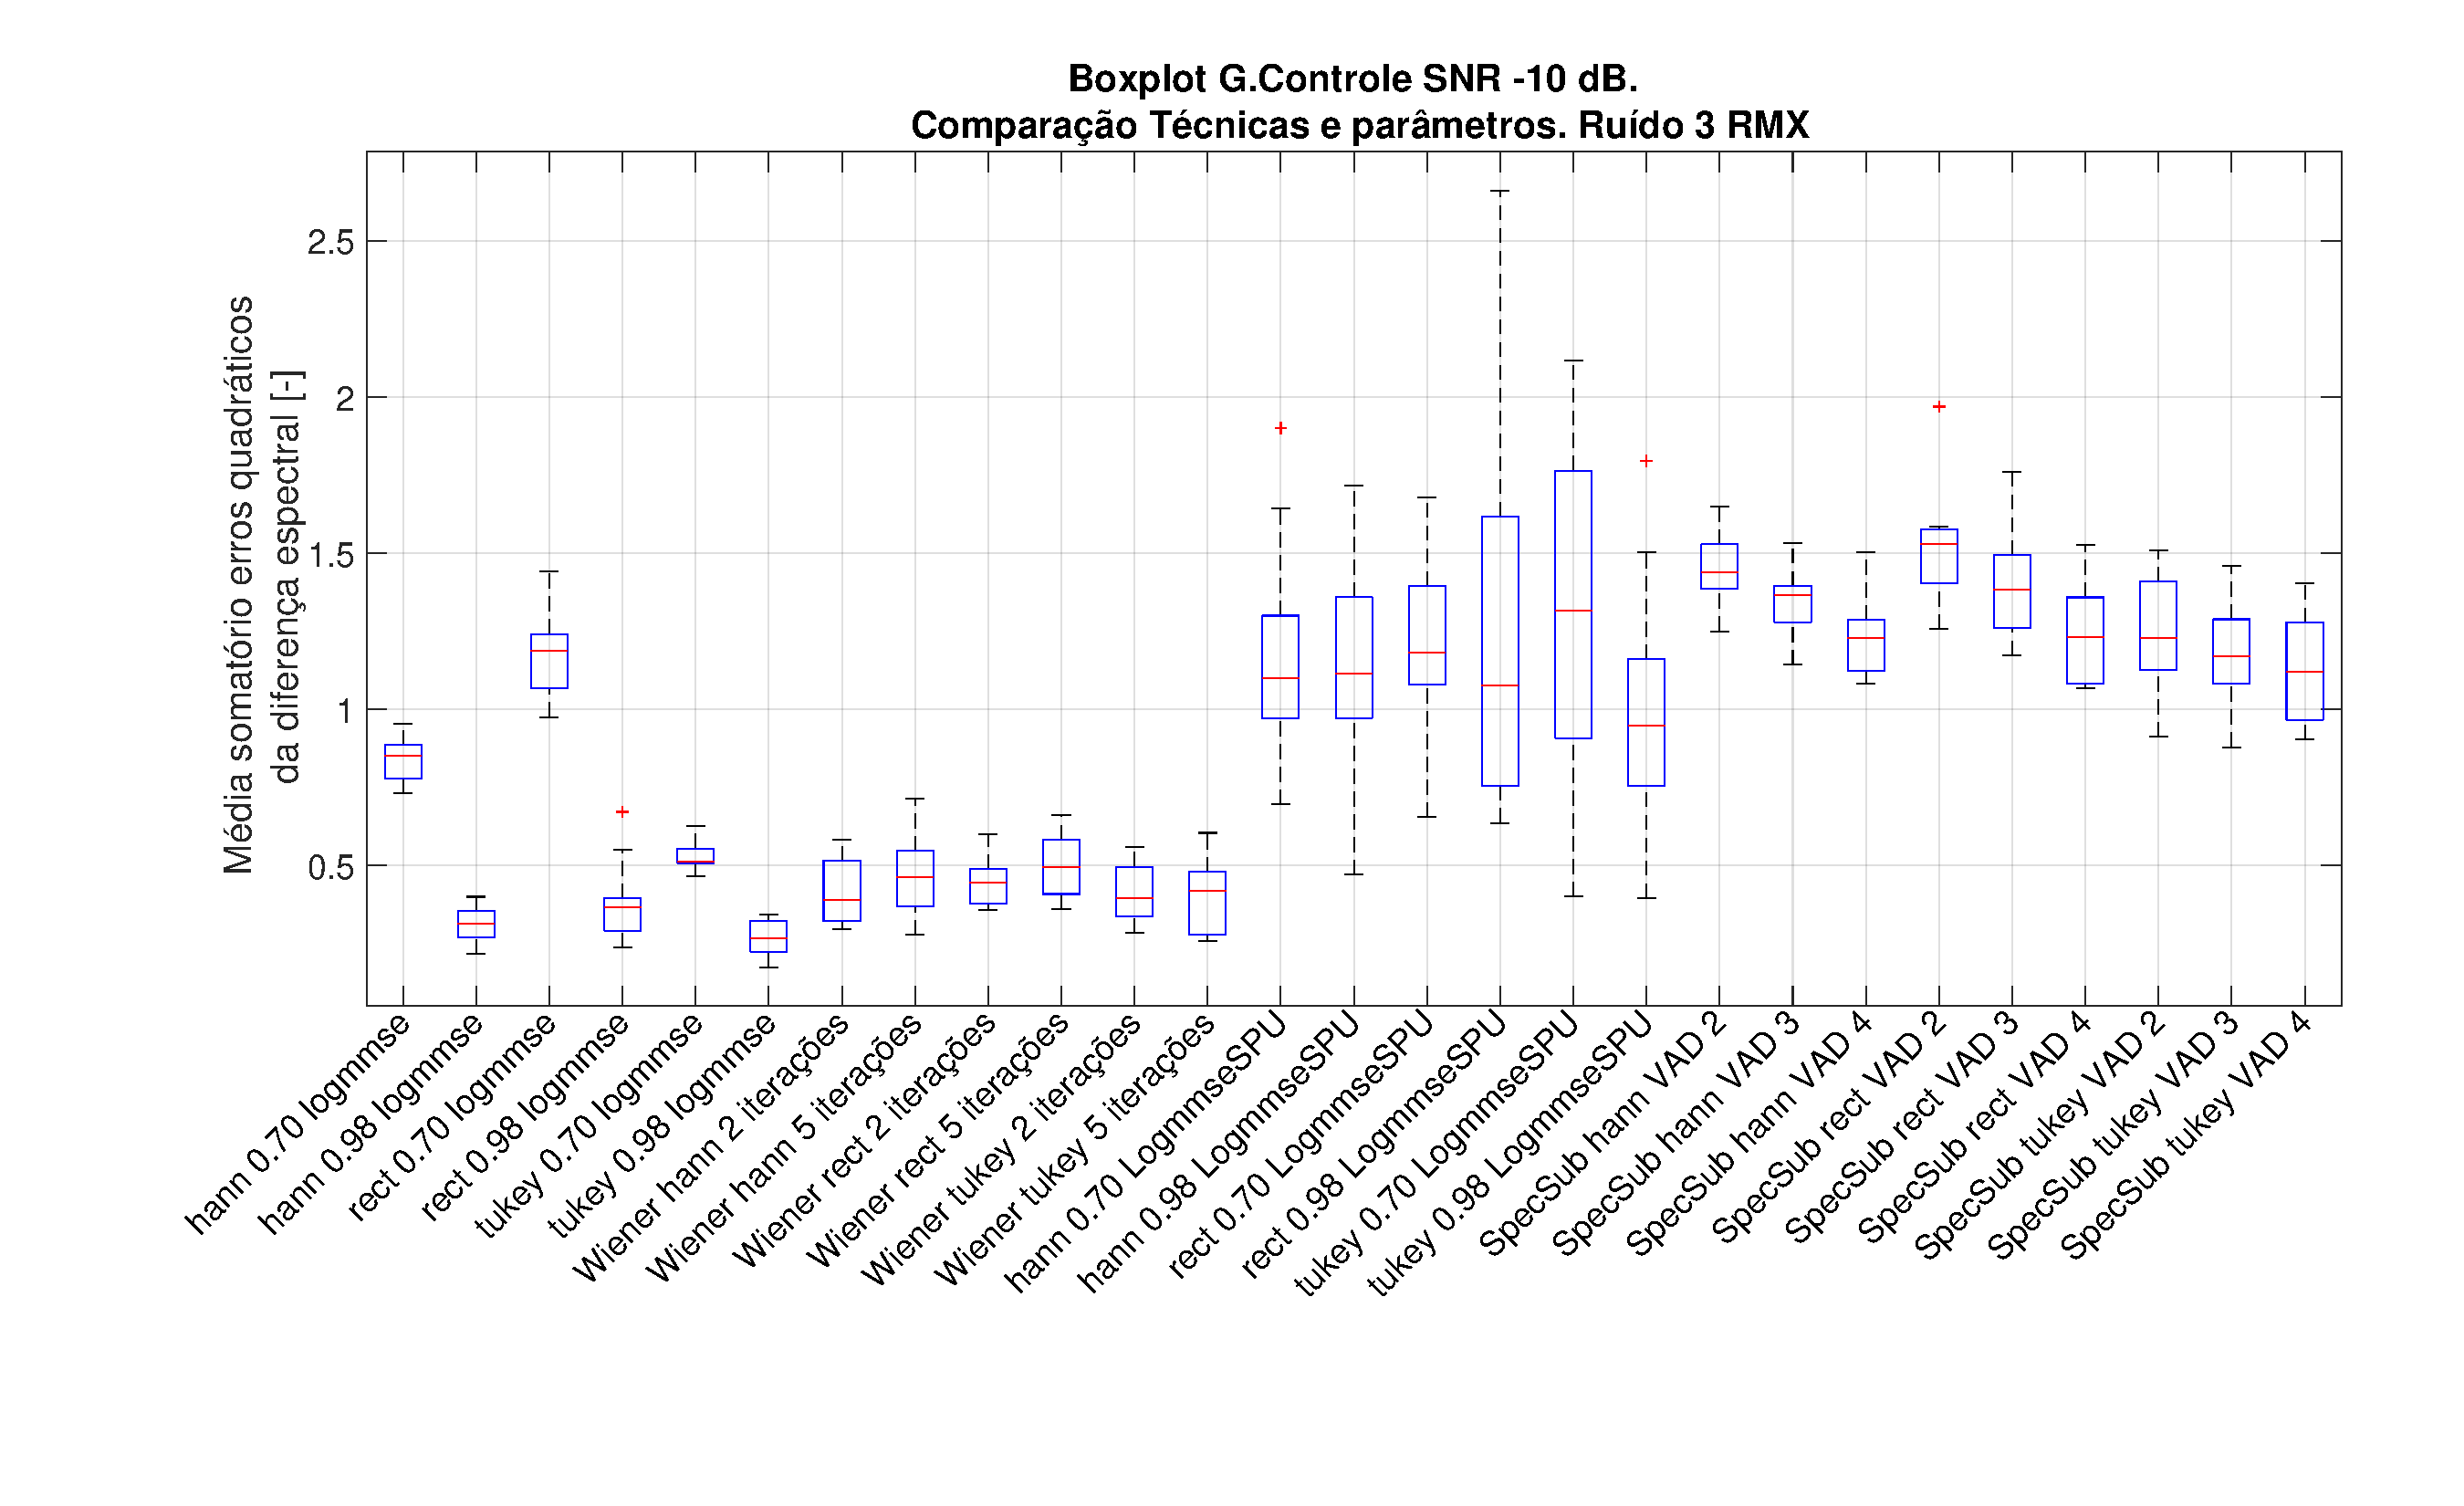
\includegraphics[width=16cm]{Figs/Erro_m10_Ruido3.pdf}
\caption{SNR -10 dB Ruído: Restaurant Mexico.}
\label{m10_3}
\end{figure}

\begin{figure}[H]
\centering
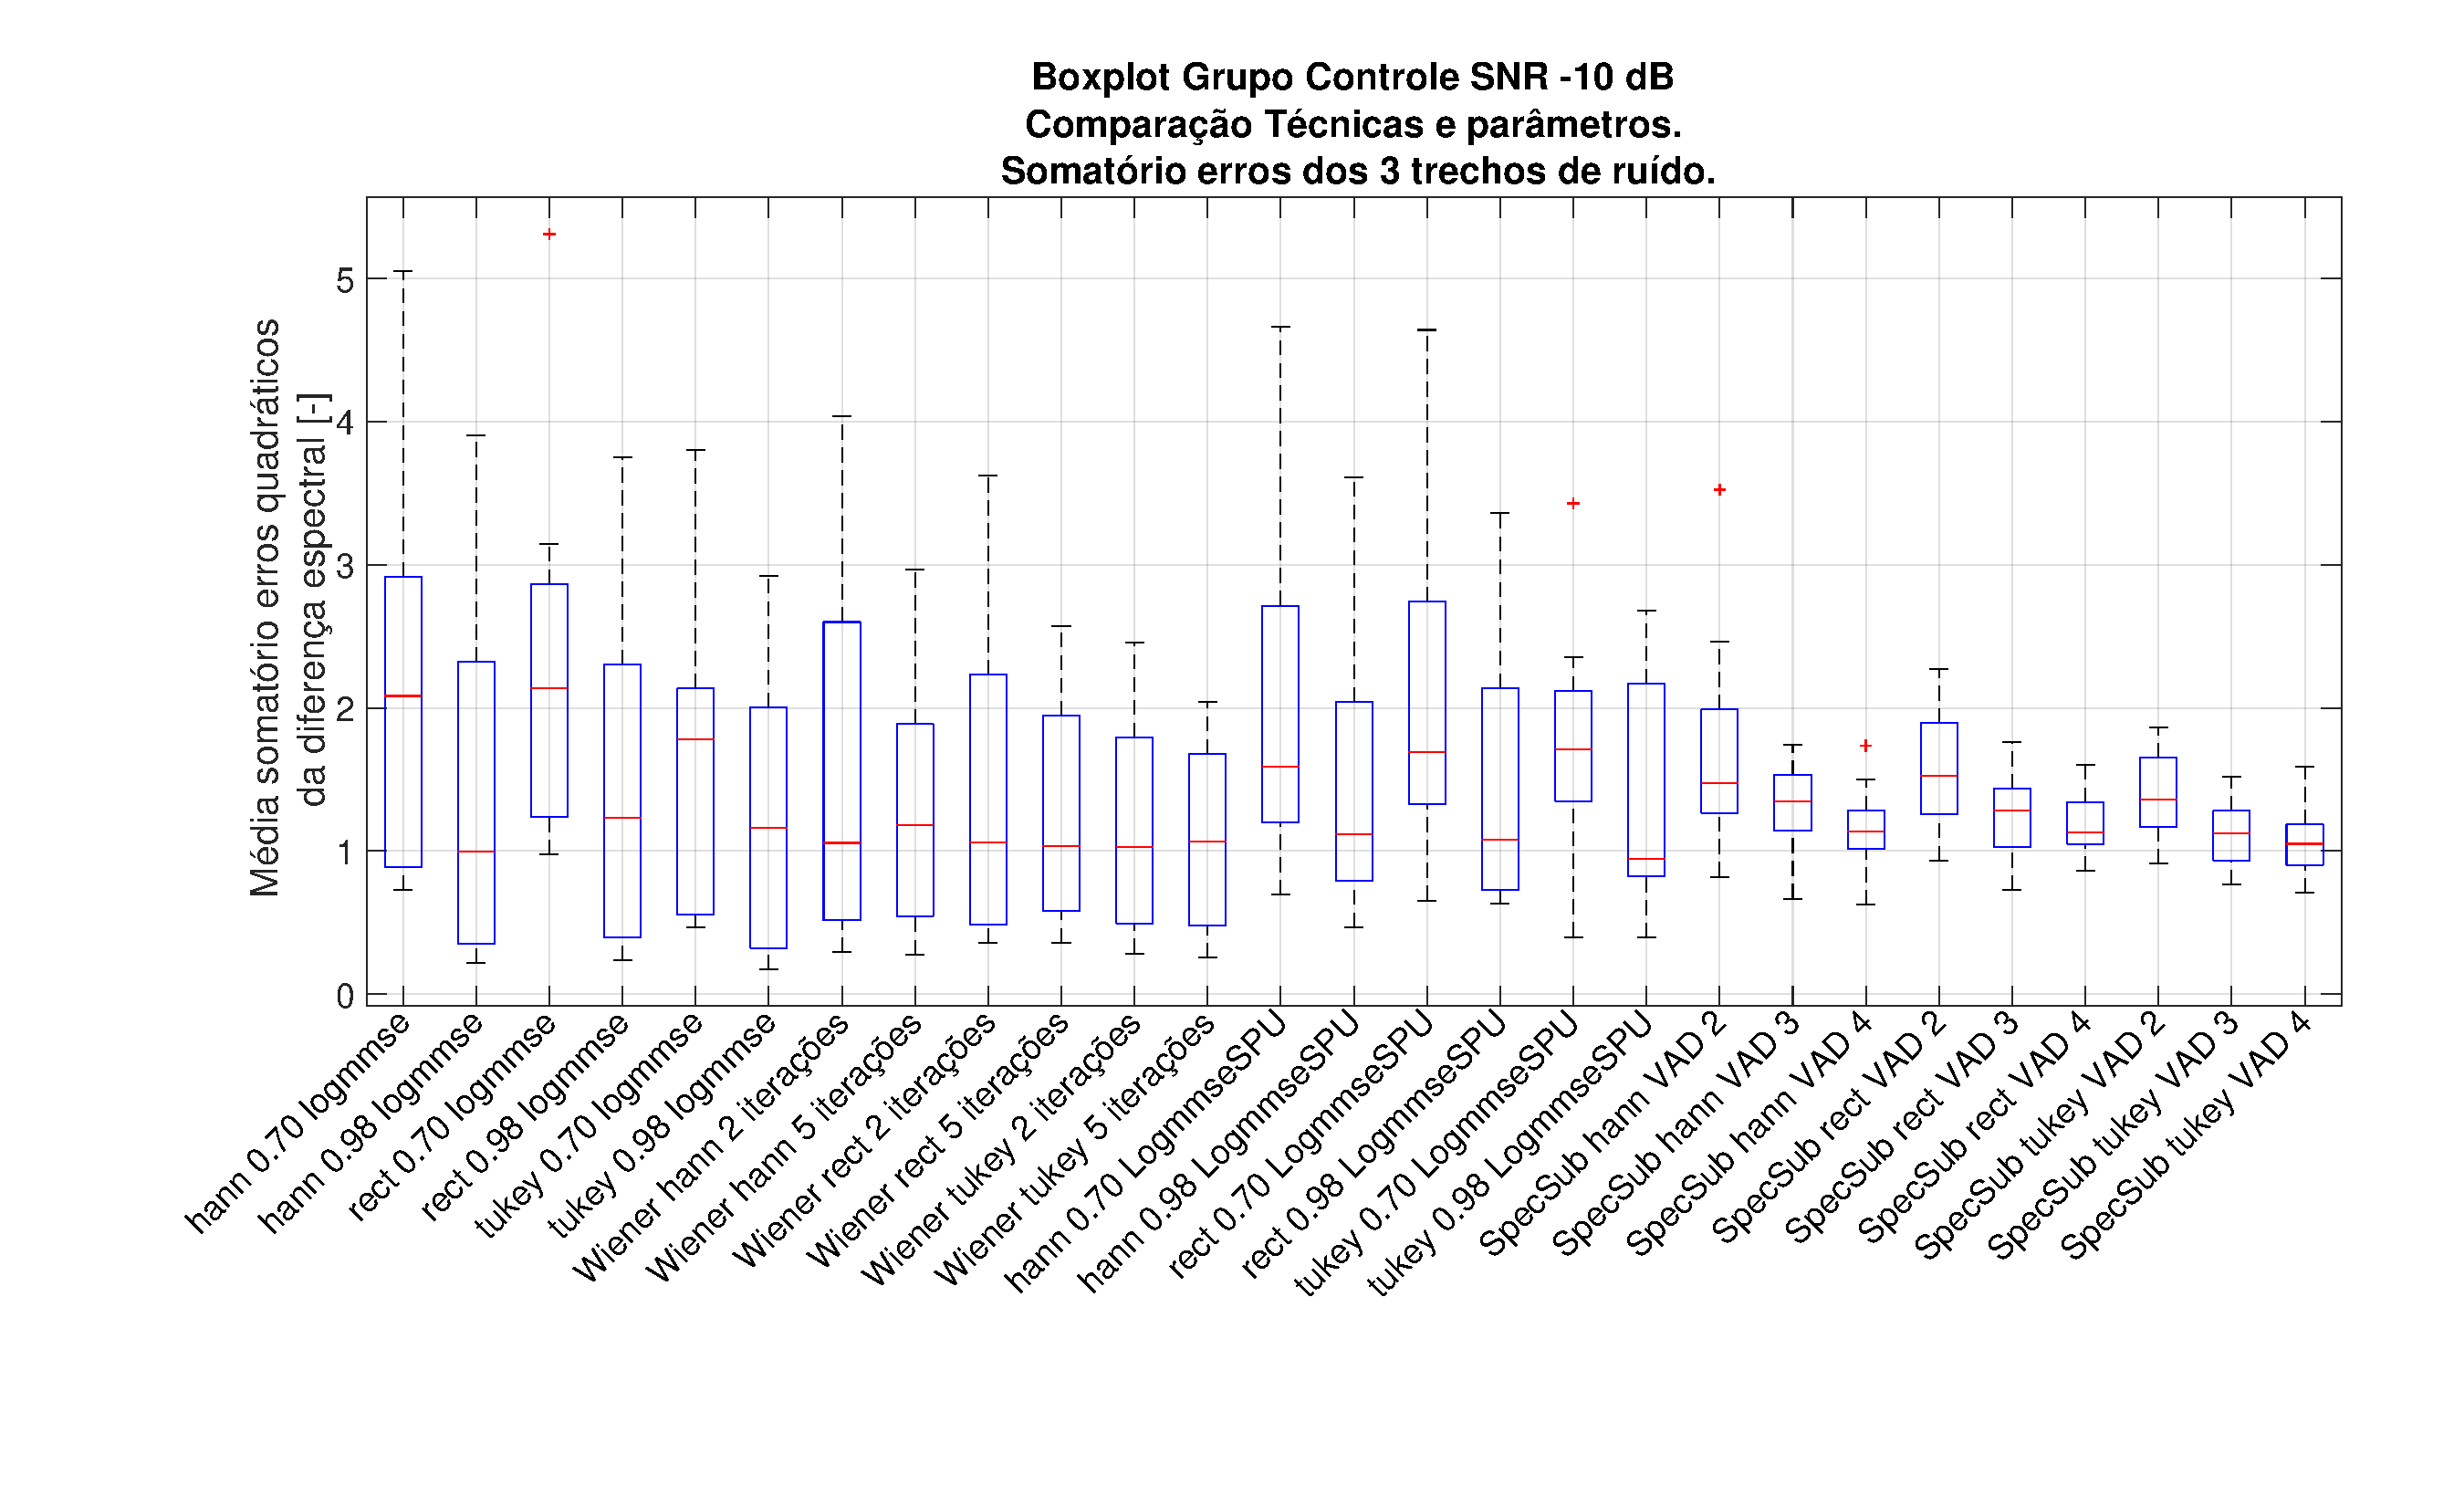
\includegraphics[width=16cm]{Figs/Erro_m10_Ruidos.pdf}
\caption{Erro SNR -10 dB todos os ruídos .}
\label{m10_3r}
\end{figure}

A \Figura{m10_3r} apresenta o conjunto de parâmetros e técnicas levando em consideração os três~ruídos, a partir desse sentido de variação de cenários acústicos a métrica da mediana do erro quadrático da subtração espectral não apresenta boa definição entre as técnicas e parâmetros.

% \begin{description}
%     \item Menor valor de mediana para o somatória dos erros quadráticos da diferença espectral considerando os 3 ruídos 
%     \item Maior  valor de mediana para o somatória dos erros quadráticos da diferença espectral considerando os 3 ruídos 
%     \item Menor e maior  valor de mediana para o somatória dos erros quadráticos da diferença espectral considerando Ruído 1 (RL) 
%     \item Menor e maior  valor de mediana para o somatória dos erros quadráticos da diferença espectral considerando Ruído 2 (RM)
%     \item Menor e maior valor de mediana para o somatória dos erros quadráticos da diferença espectral considerando Ruído 3 (RMX)
% \end{description}


% \begin{table}[H]
% \centering
% \caption{Valores de mediana para o somatória dos erros quadráticos da diferença espectral entre sinal processado e sinal original.}
% \label{tabela-10}
% \resizebox{\textwidth}{!}{%
% \begin{tabular}{cccc}
% \rowcolor[HTML]{FFFFC7} 
% \multicolumn{4}{c}{\cellcolor[HTML]{FFFFC7}Mediana da somatória dos erros quadráticos da diferença espectral SNR = -10 dB} \\\hline
% \rowcolor[HTML]{ECF4FF} 
% \begin{tabular}[c]{@{}c@{}}Ruído 1 \\ Babbel noise + música\end{tabular} & \begin{tabular}[c]{@{}c@{}}Ruído 2 \\ Babbel noise\end{tabular} & \begin{tabular}[c]{@{}c@{}}Ruído 3 \\ Música pronunciada\end{tabular} & Ruídos combinados \\
% \rowcolor[HTML]{FFCCC9} 
% \begin{tabular}[c]{@{}c@{}}Logmmse Han 0,70\\ Valor = 2,987\end{tabular} & \begin{tabular}[c]{@{}c@{}}Logmmse Rect 0,70\\ Valor = 2,1803\end{tabular} & \begin{tabular}[c]{@{}c@{}}SpecSub Rect VAD 2 \\ Valor = 1,5300\end{tabular} & \begin{tabular}[c]{@{}c@{}}Logmmse Rect 0,70\\ Valor = 2,1372\end{tabular} \\
% \rowcolor[HTML]{ECF4FF} 
% \begin{tabular}[c]{@{}c@{}}SpecSub Tukey VAD 4\\ Valor = 1,1683\end{tabular} & \begin{tabular}[c]{@{}c@{}}Logmmse SPU Rect 0,98\\ Valor = 0,7169\end{tabular} & \begin{tabular}[c]{@{}c@{}}Logmmse Tukey 0,98\\ Valor = 0,26817\end{tabular} & \begin{tabular}[c]{@{}c@{}}Logmmse Hann 0,98\\ Valor = 0,9965\end{tabular}
% \end{tabular}
% }
% \end{table}

%%%%%%%%%%%%%%%%%%%%%%%%%%%%%%%%%%%%%%%%%%%%%%%%%%%%%%%%%%%%%%%%%%%%%%%%%%%%%%%%%%%%%%%%%%%%%%%%%%%%%%%%%%%%%%%%%%%%%%%%%% SNR 0 SNR 0 SNR 0 SNR 0 SNR 0 SNR 0 SNR 0 SNR 0 SNR 0 SNR 0 SNR 0 SNR 0 SNR 0 SNR 0 SNR 0 SNR 0 SNR 0 SNR 0 SNR 0 SNR 0 SNR 0 SNR 0 SNR 0 SNR 0 SNR 0 SNR 0 SNR 0 SNR 0 SNR 0 SNR 0 SNR 0 SNR 0 SNR 0 SNR 0 SNR 0 SNR 0 

\subsubsection{Análise da eficiência das técnicas para SNR 0 dB}


A \figura{snr0_1} apresenta o \textit{vs} da média do somatório dos erros quadráticos da diferença entre o sinal processado pelas técnicas escolhidas, com a variação dos parâmetros mencionados, para a relação sinal ruído de 0 dB e com o ruído contaminante RL.

\begin{figure}[H]
\centering
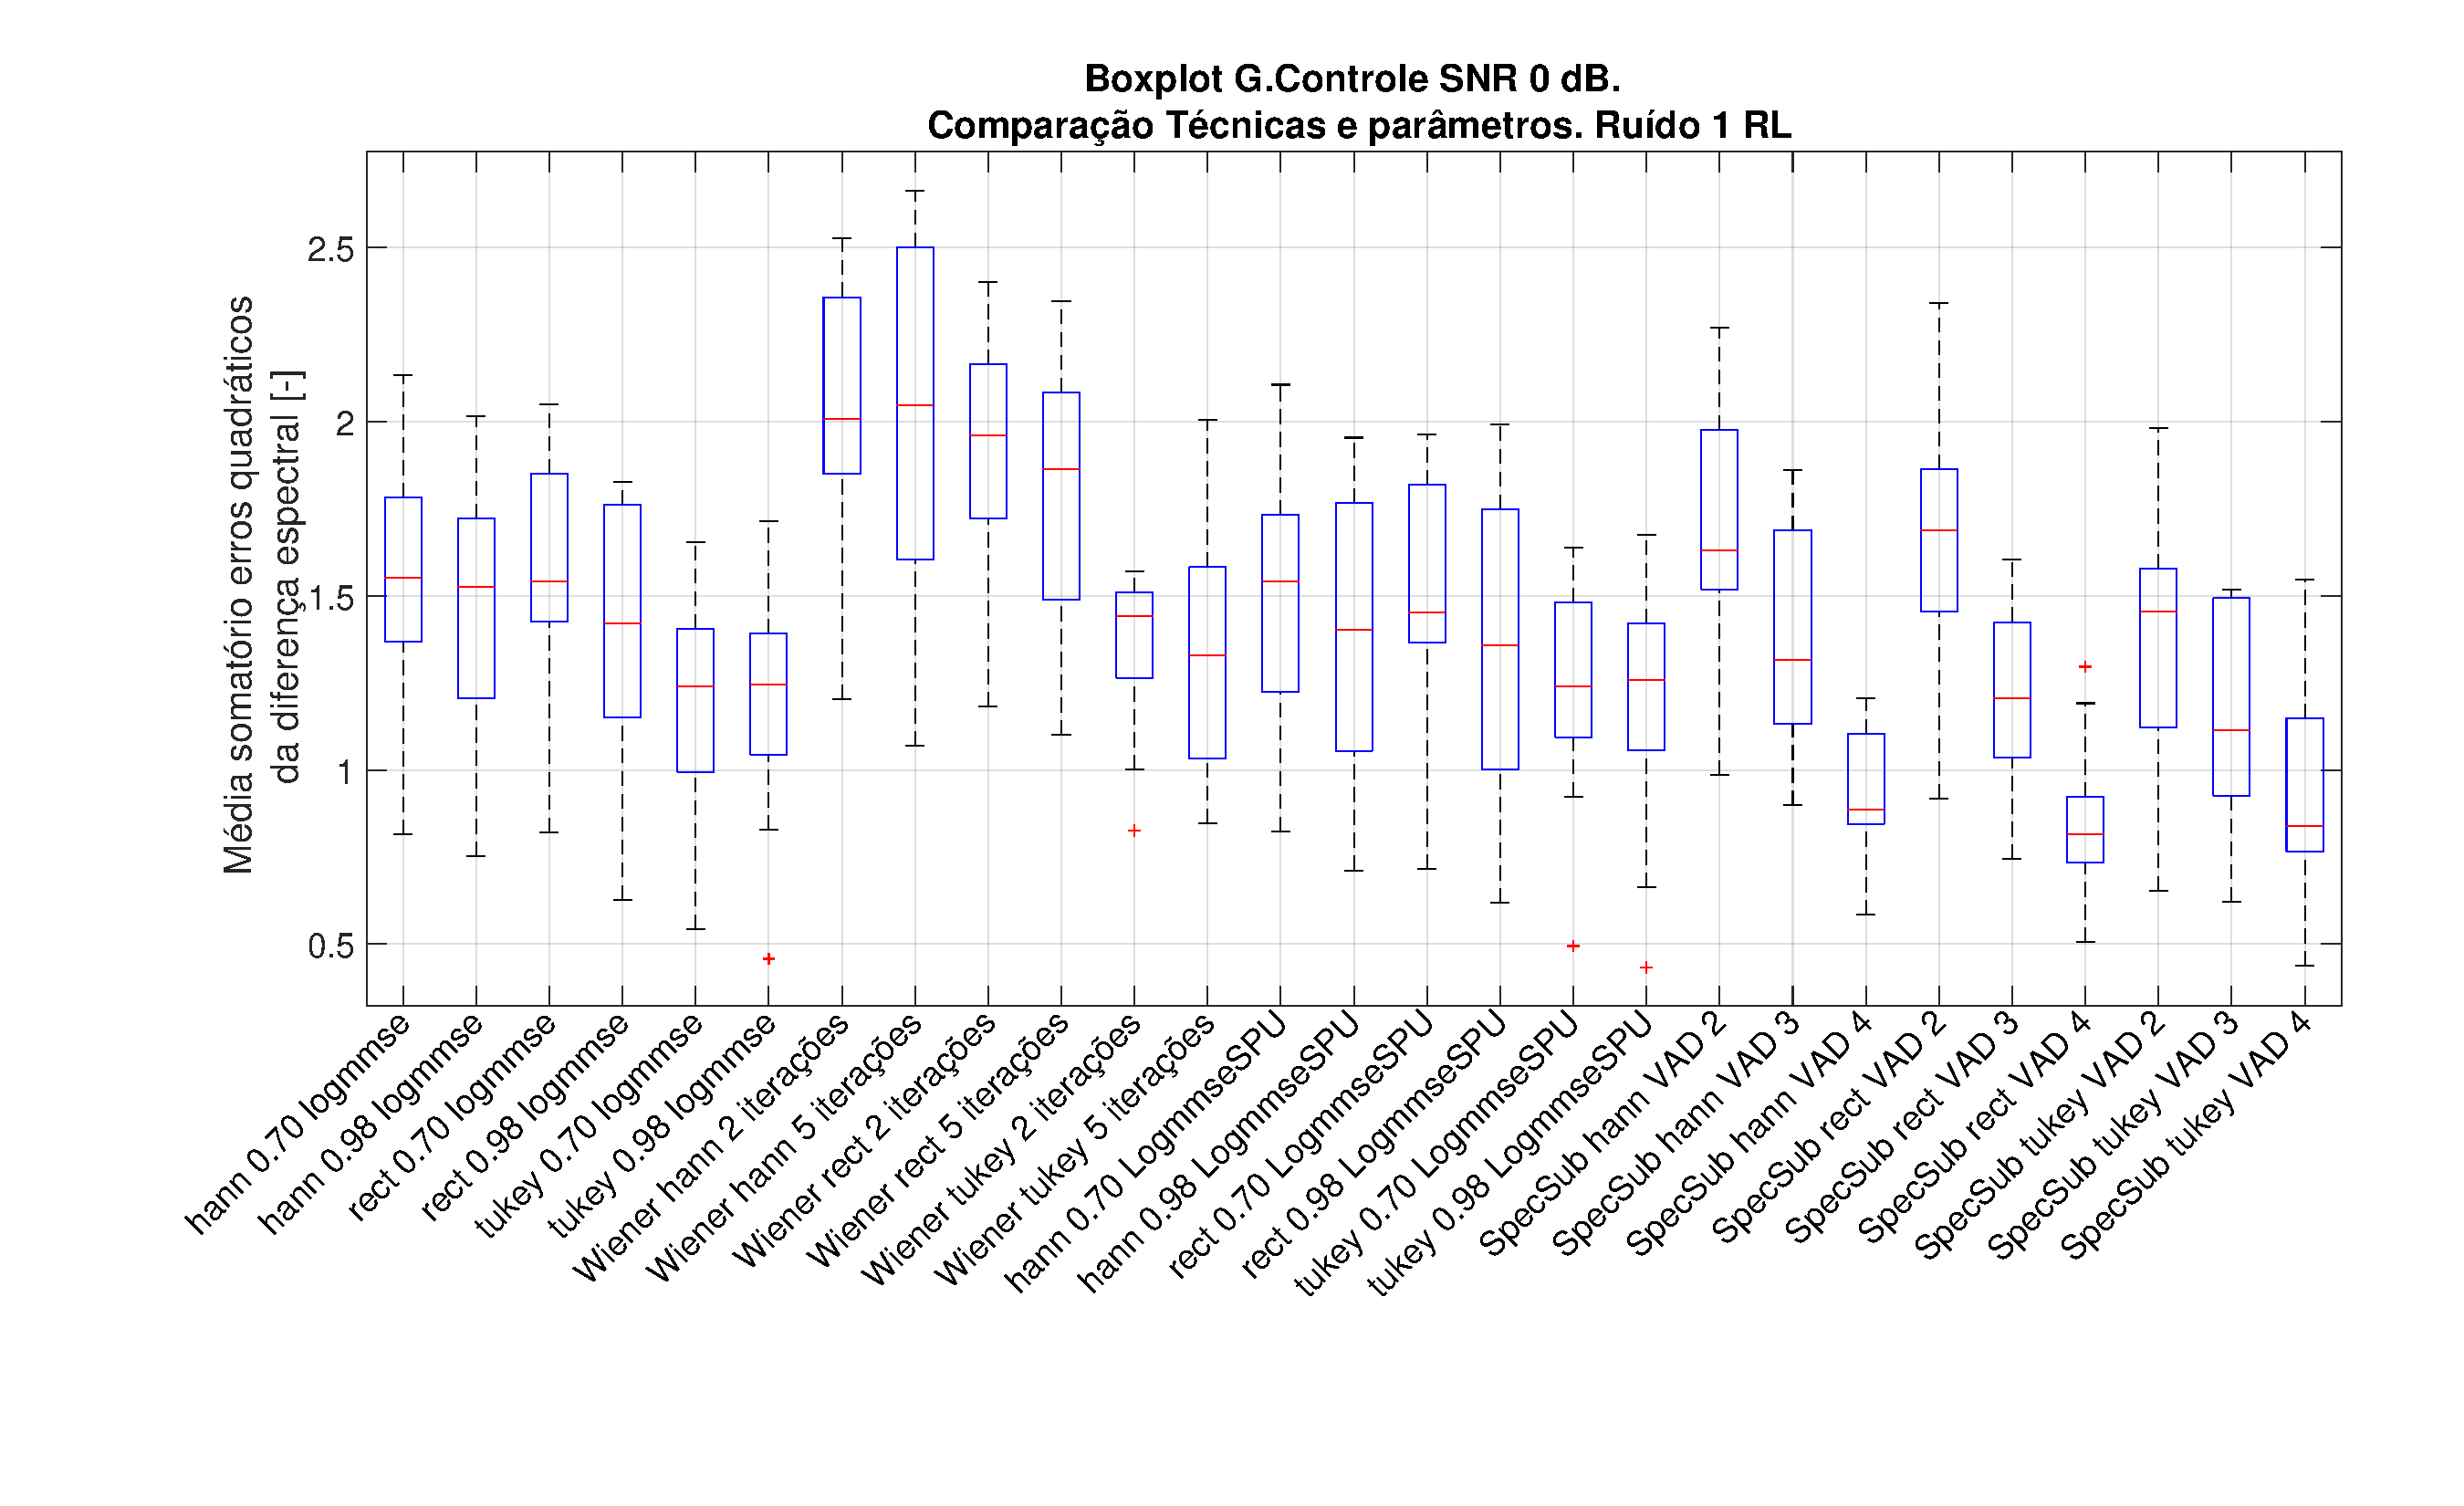
\includegraphics[width=16cm]{Figs/Erro_0_Ruido1.pdf}
\caption{SNR 0 dB Ruído: Restaurant Large.}
\label{snr0_1}
\end{figure}

As \figuras{snr0_2} e \ref{snr0_3} apresentam as mesmas variáveis, contudo para o ruído contaminante RM e RMX respectivamente.

\begin{figure}[H]
\centering
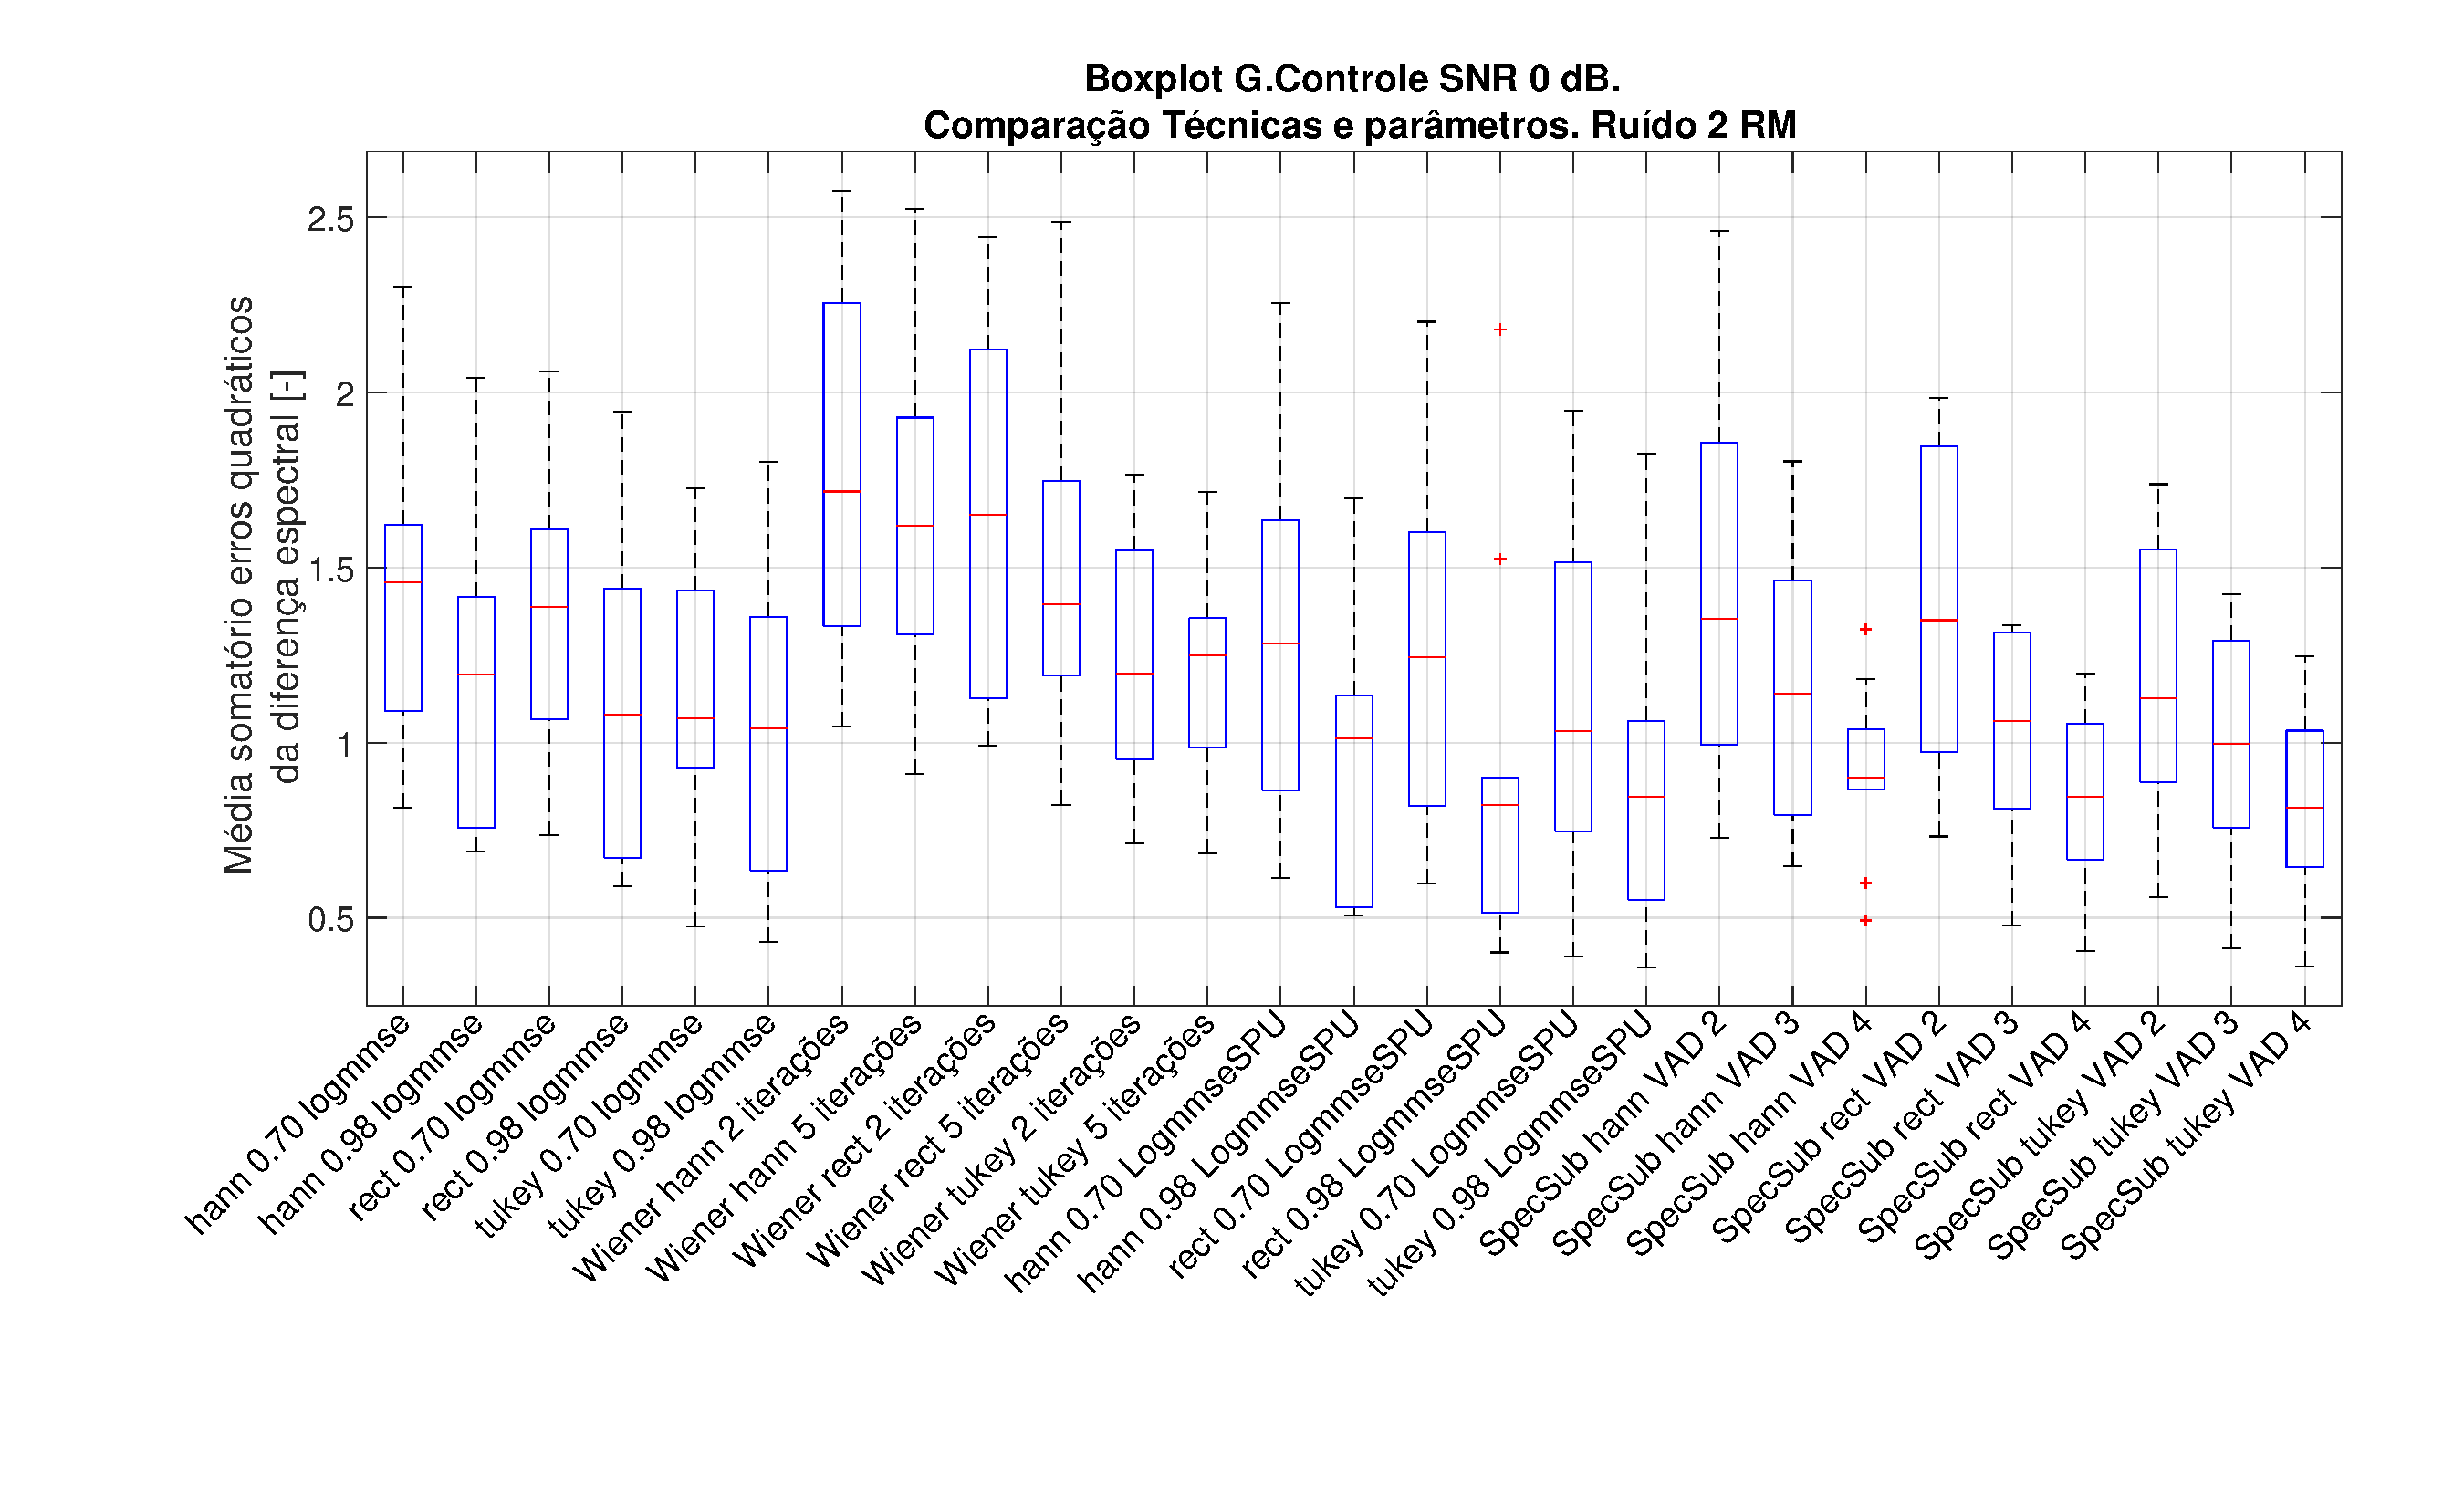
\includegraphics[width=16cm]{Figs/Erro_0_Ruido2.pdf} 
\caption{SNR 0 dB Ruído: Restaurant medium.}
\label{snr0_2}
\end{figure}

\begin{figure}[H]
\centering
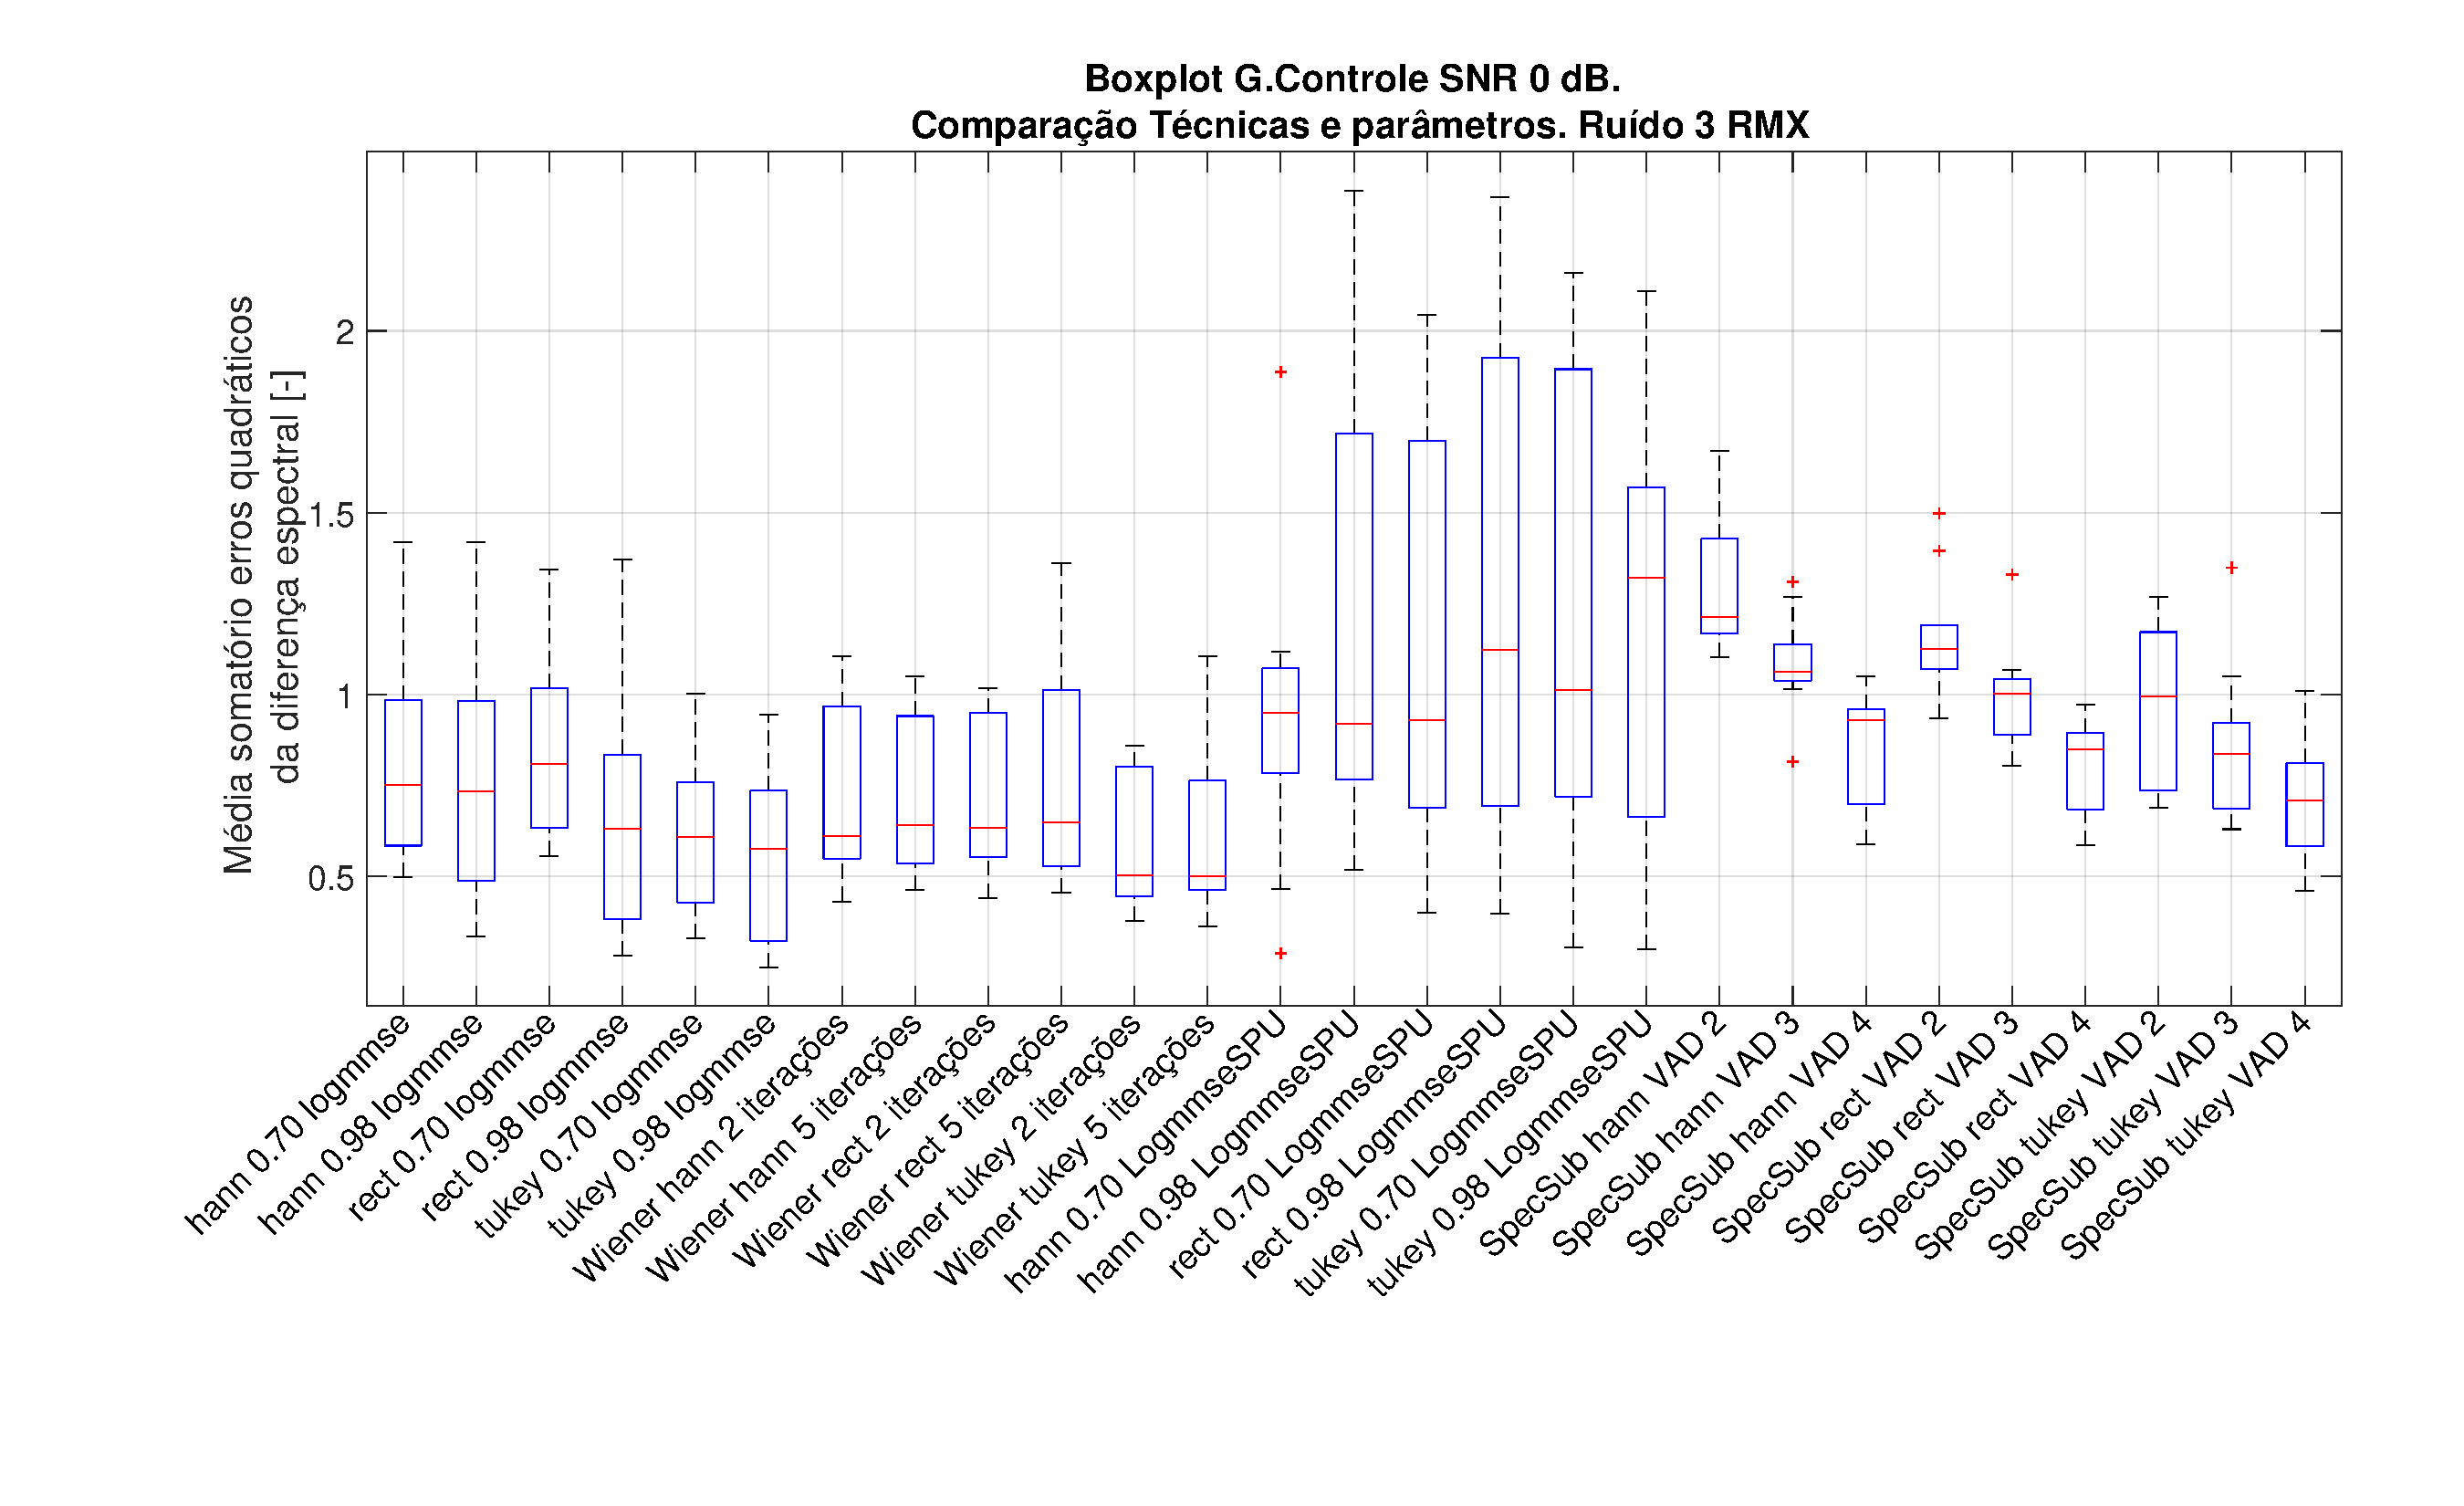
\includegraphics[width=16cm]{Figs/Erro_0_Ruido3.pdf}
\caption{SNR 0 dB Ruído: Restaurant Mexico.}
\label{snr0_3}
\end{figure}

Em uma primeira análise, com o incremento da relação sinal ruído a técnica de filtragem de Wiener apresenta maiores valores de mediana para o erro médio quadrático para o ruído RL, ver \figura{snr0_1} e para o ruído RM, ver \figura{snr0_2}. O ruído RL tem características de \textit{babble noise} e música ao fundo, enquanto o ruído RM é basicamente composto de \textit{babble noise}. Esse efeito não se repete no ruído RMX, ver \figura{snr0_3}, onde a característica predominante é uma música tocada ao violão com fundo de \textit{babble noise}. As características do ruído mais uma vez apareceram como discrepantes na utilização do método de avaliar o erro médio quadrático da subtração espectral e podem ter efeitos na observação subjetiva dos sinais quando os sinais contaminados por um ruído com característica for processado por uma técnica com parâmetros ajustados para outro ruído com características diferentes.  

\begin{figure}[H]
\centering
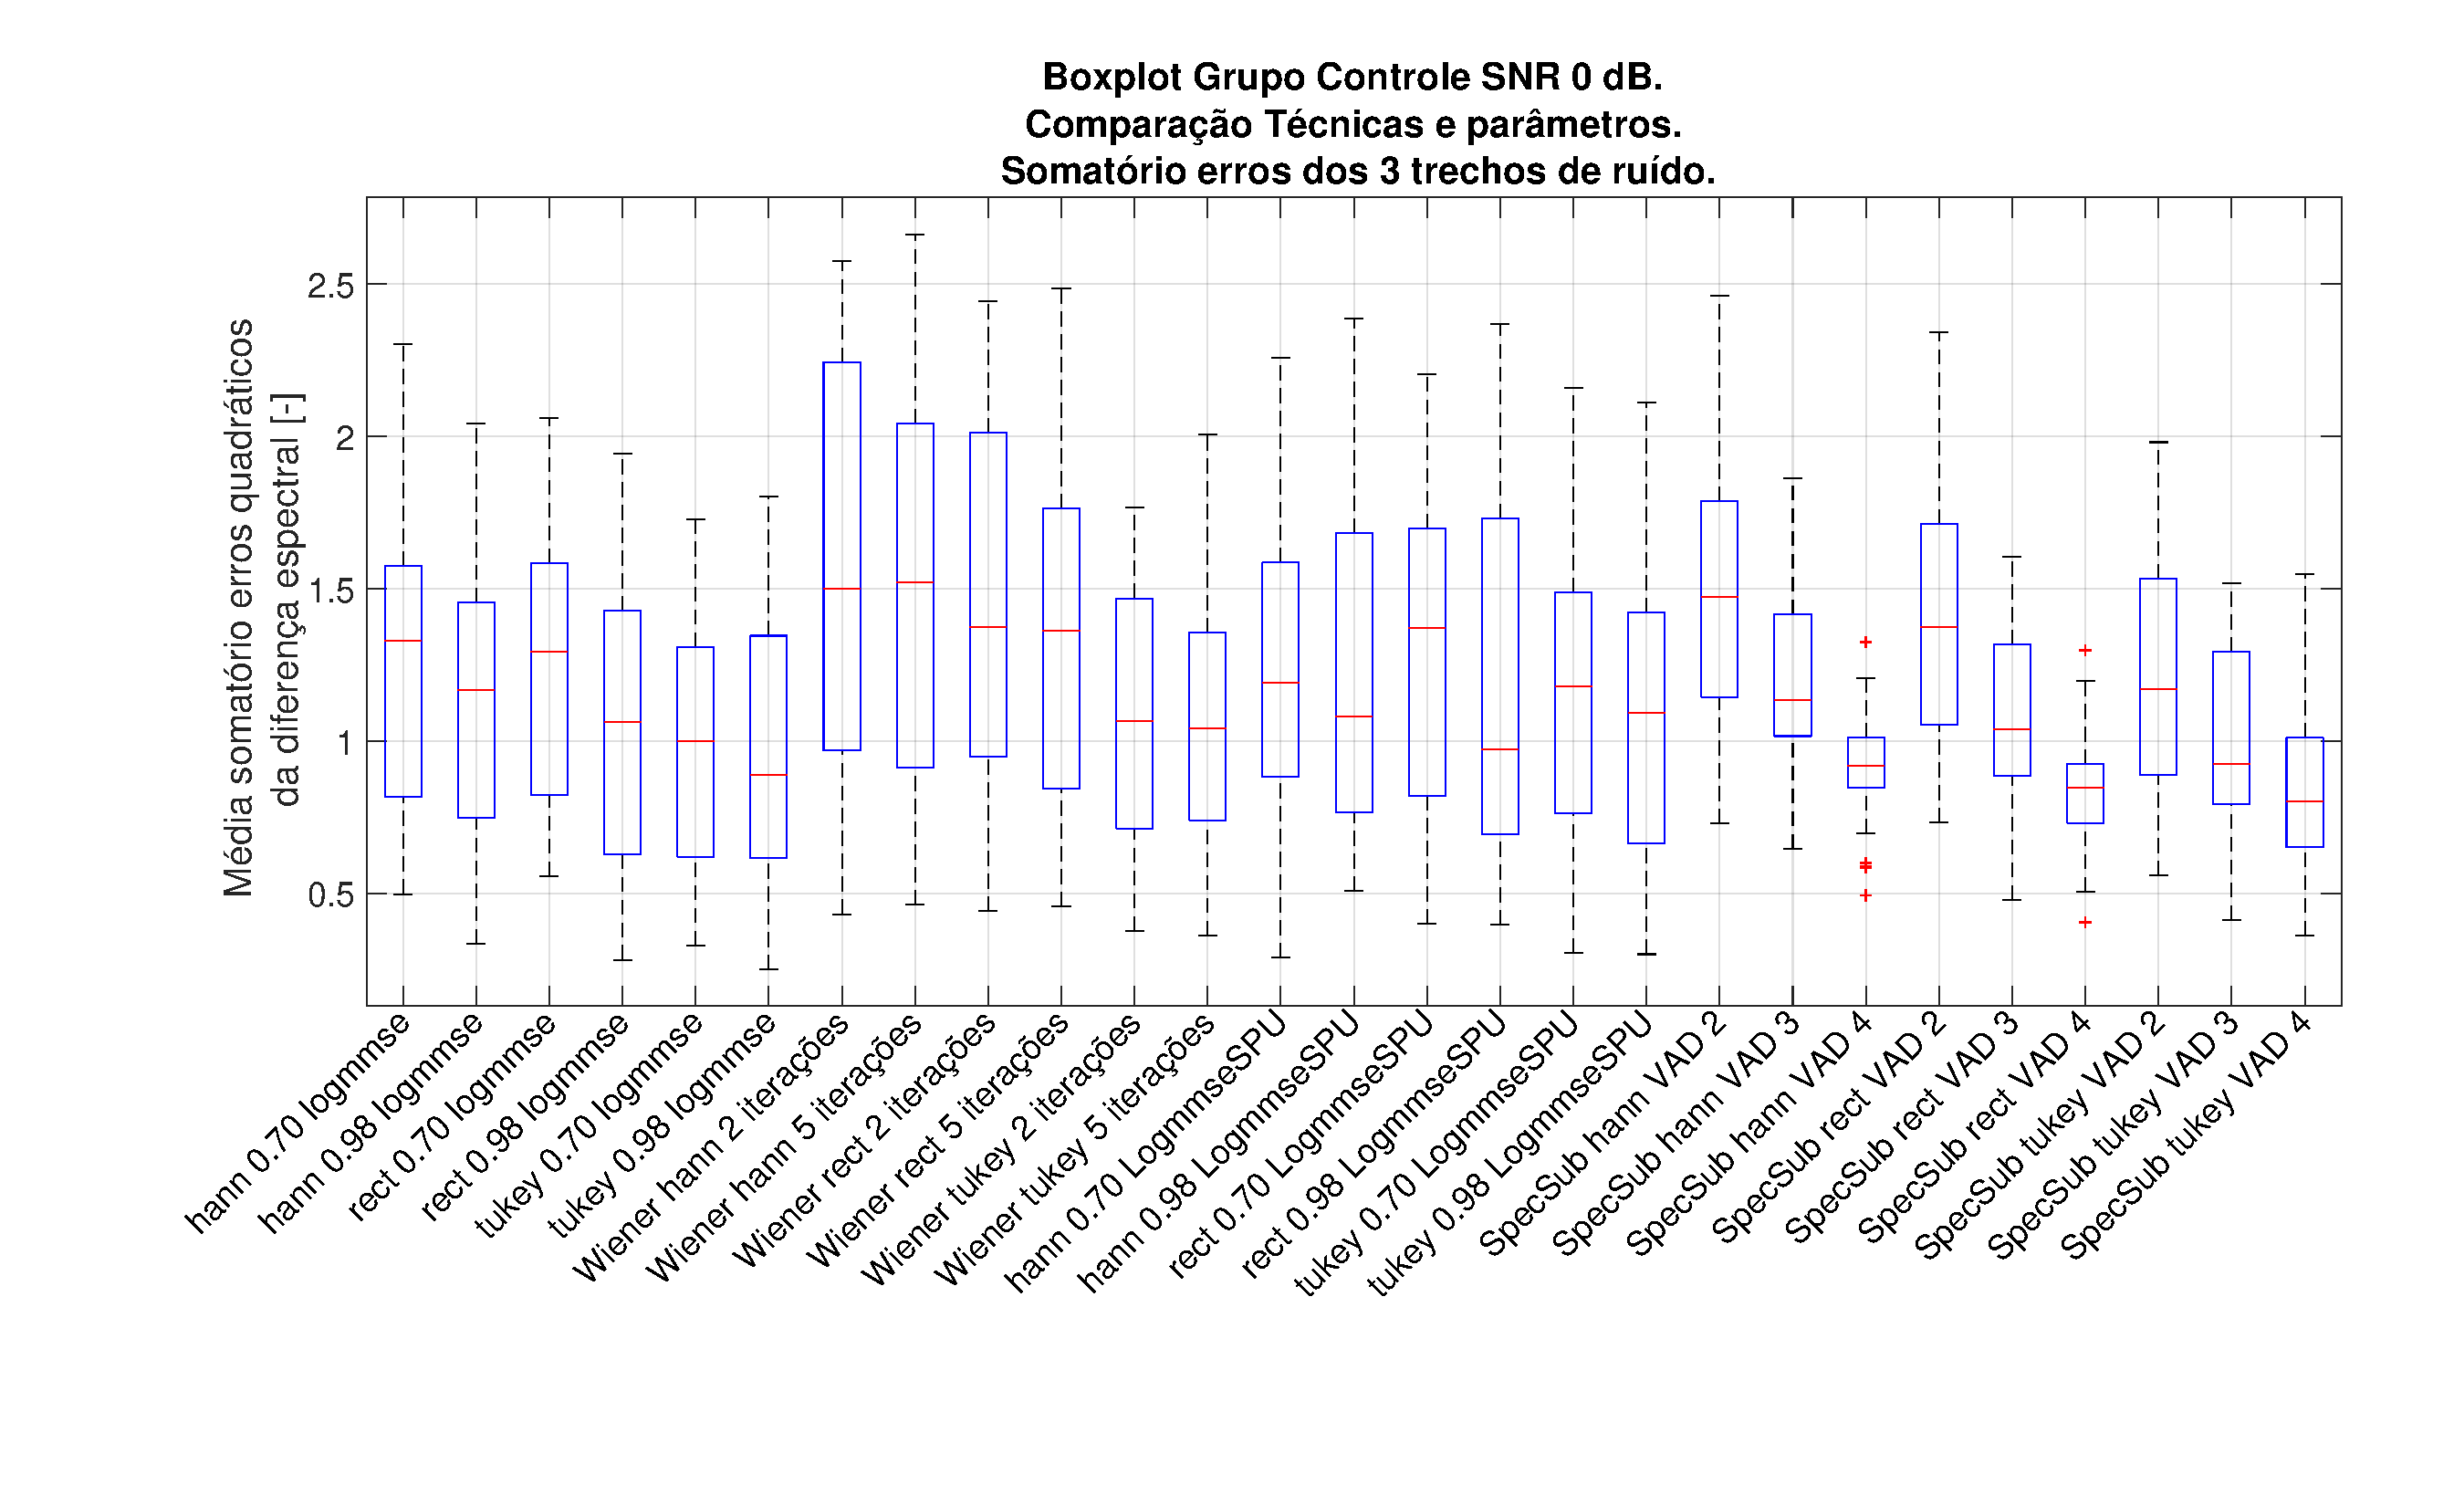
\includegraphics[width=16cm]{Figs/Erro_0_Ruidos.pdf}
\caption{Erro SNR 0 dB todos os ruídos .}
\label{snr0_3r}
\end{figure}

a \figura{snr0_3r} apresenta os valores de erro médio quadrático tomando em consideração o espaço amostral dos 3 ruídos contaminantes. Assim a definição dos parâmetros de cada técnica será selecionada não para um ruído em específico, e sim para a mediana que representa um número maior de amostras.



% Please add the following required packages to your document preamble:
% \usepackage{graphicx}
% \usepackage[table,xcdraw]{xcolor}
% If you use beamer only pass "xcolor=table" option, i.e. \documentclass[xcolor=table]{beamer}
% \begin{table}[H]
% \centering
% \caption{Valores de mediana para o somatória dos erros quadráticos da diferença espectral entre sinal processado e sinal original.}
% \label{tabela0}
% \resizebox{\textwidth}{!}{%
% \begin{tabular}{cccc}
% \rowcolor[HTML]{FFFFC7} 
% \multicolumn{4}{c}{\cellcolor[HTML]{FFFFC7}Mediana da somatória dos erros quadráticos da diferença espectral SNR = 0 dB}                                                                                                                                                                                                    \\
% \rowcolor[HTML]{ECF4FF} 
% \begin{tabular}[c]{@{}c@{}}Ruído 1 \\ Babbel noise + música\end{tabular}    & \begin{tabular}[c]{@{}c@{}}Ruído 2 \\ Babbel noise\end{tabular}              & \begin{tabular}[c]{@{}c@{}}Ruído 3 \\ Música pronunciada\end{tabular}           & Ruídos combinados                                                            \\
% \rowcolor[HTML]{FFCCC9} 
% \begin{tabular}[c]{@{}c@{}}Wienner Han 5 iter\\ Valor = 2,0464\end{tabular} & \begin{tabular}[c]{@{}c@{}}Wienner Han 2 iter\\ Valor = 1,7176\end{tabular}  & \begin{tabular}[c]{@{}c@{}}Logmmse SPU Tukey 0,98\\ Valor = 1,3208\end{tabular} & \begin{tabular}[c]{@{}c@{}}Wienner Han 5 iter\\ Valor = 1,5205\end{tabular}  \\
% \rowcolor[HTML]{ECF4FF} %%
% \begin{tabular}[c]{@{}c@{}}SpecSub Rect VAD 4\\ Valor = 0,8156\end{tabular} & \begin{tabular}[c]{@{}c@{}}SpecSub Tukey VAD 4\\ Valor = 0,8138\end{tabular} & \begin{tabular}[c]{@{}c@{}}Wienner Tukey 5 iter\\ Valor = 0,4994\end{tabular}   & \begin{tabular}[c]{@{}c@{}}SpecSub Tukey VAD 4\\ Valor = 0,8018\end{tabular}
% \end{tabular}%
% }
% \end{table}
%%%%%%%%%%%%%%%%%%%%%%%%%%%%%%%%%%%%%%%%%%%%%%%%%%%%%%%%%%%%%%%%%%%%%%%%%%%%%%%%%%%%%%%%%%%%%%%%%%%%%%%%%%%%%%%%%%%%%%%%%% SNR 10 %%%%%%%%%%%%%%%%%%%%%%%%%%%%%%%%%%%%%%%%%%%%%%%%%%%%%%%%%%%%%%%%%%%%%%%%%%%%%%%%%%%%%%%%%%%%%%%%%%%%%%%%%%%%%%%%%%%%%%%%% 


\subsubsection{Análise da eficiência das técnicas para SNR 10 dB}


Como nas seções anteriores, a \figura{snr10_1} apresenta o boxplot da média do somatório dos erros médios quadráticos da diferença entre o sinal processado pelas técnicas escolhidas, com a variação dos parâmetros mencionados, para a relação sinal ruído de -10 dB e com o ruído contaminante RL.

\begin{figure}[H]
\centering
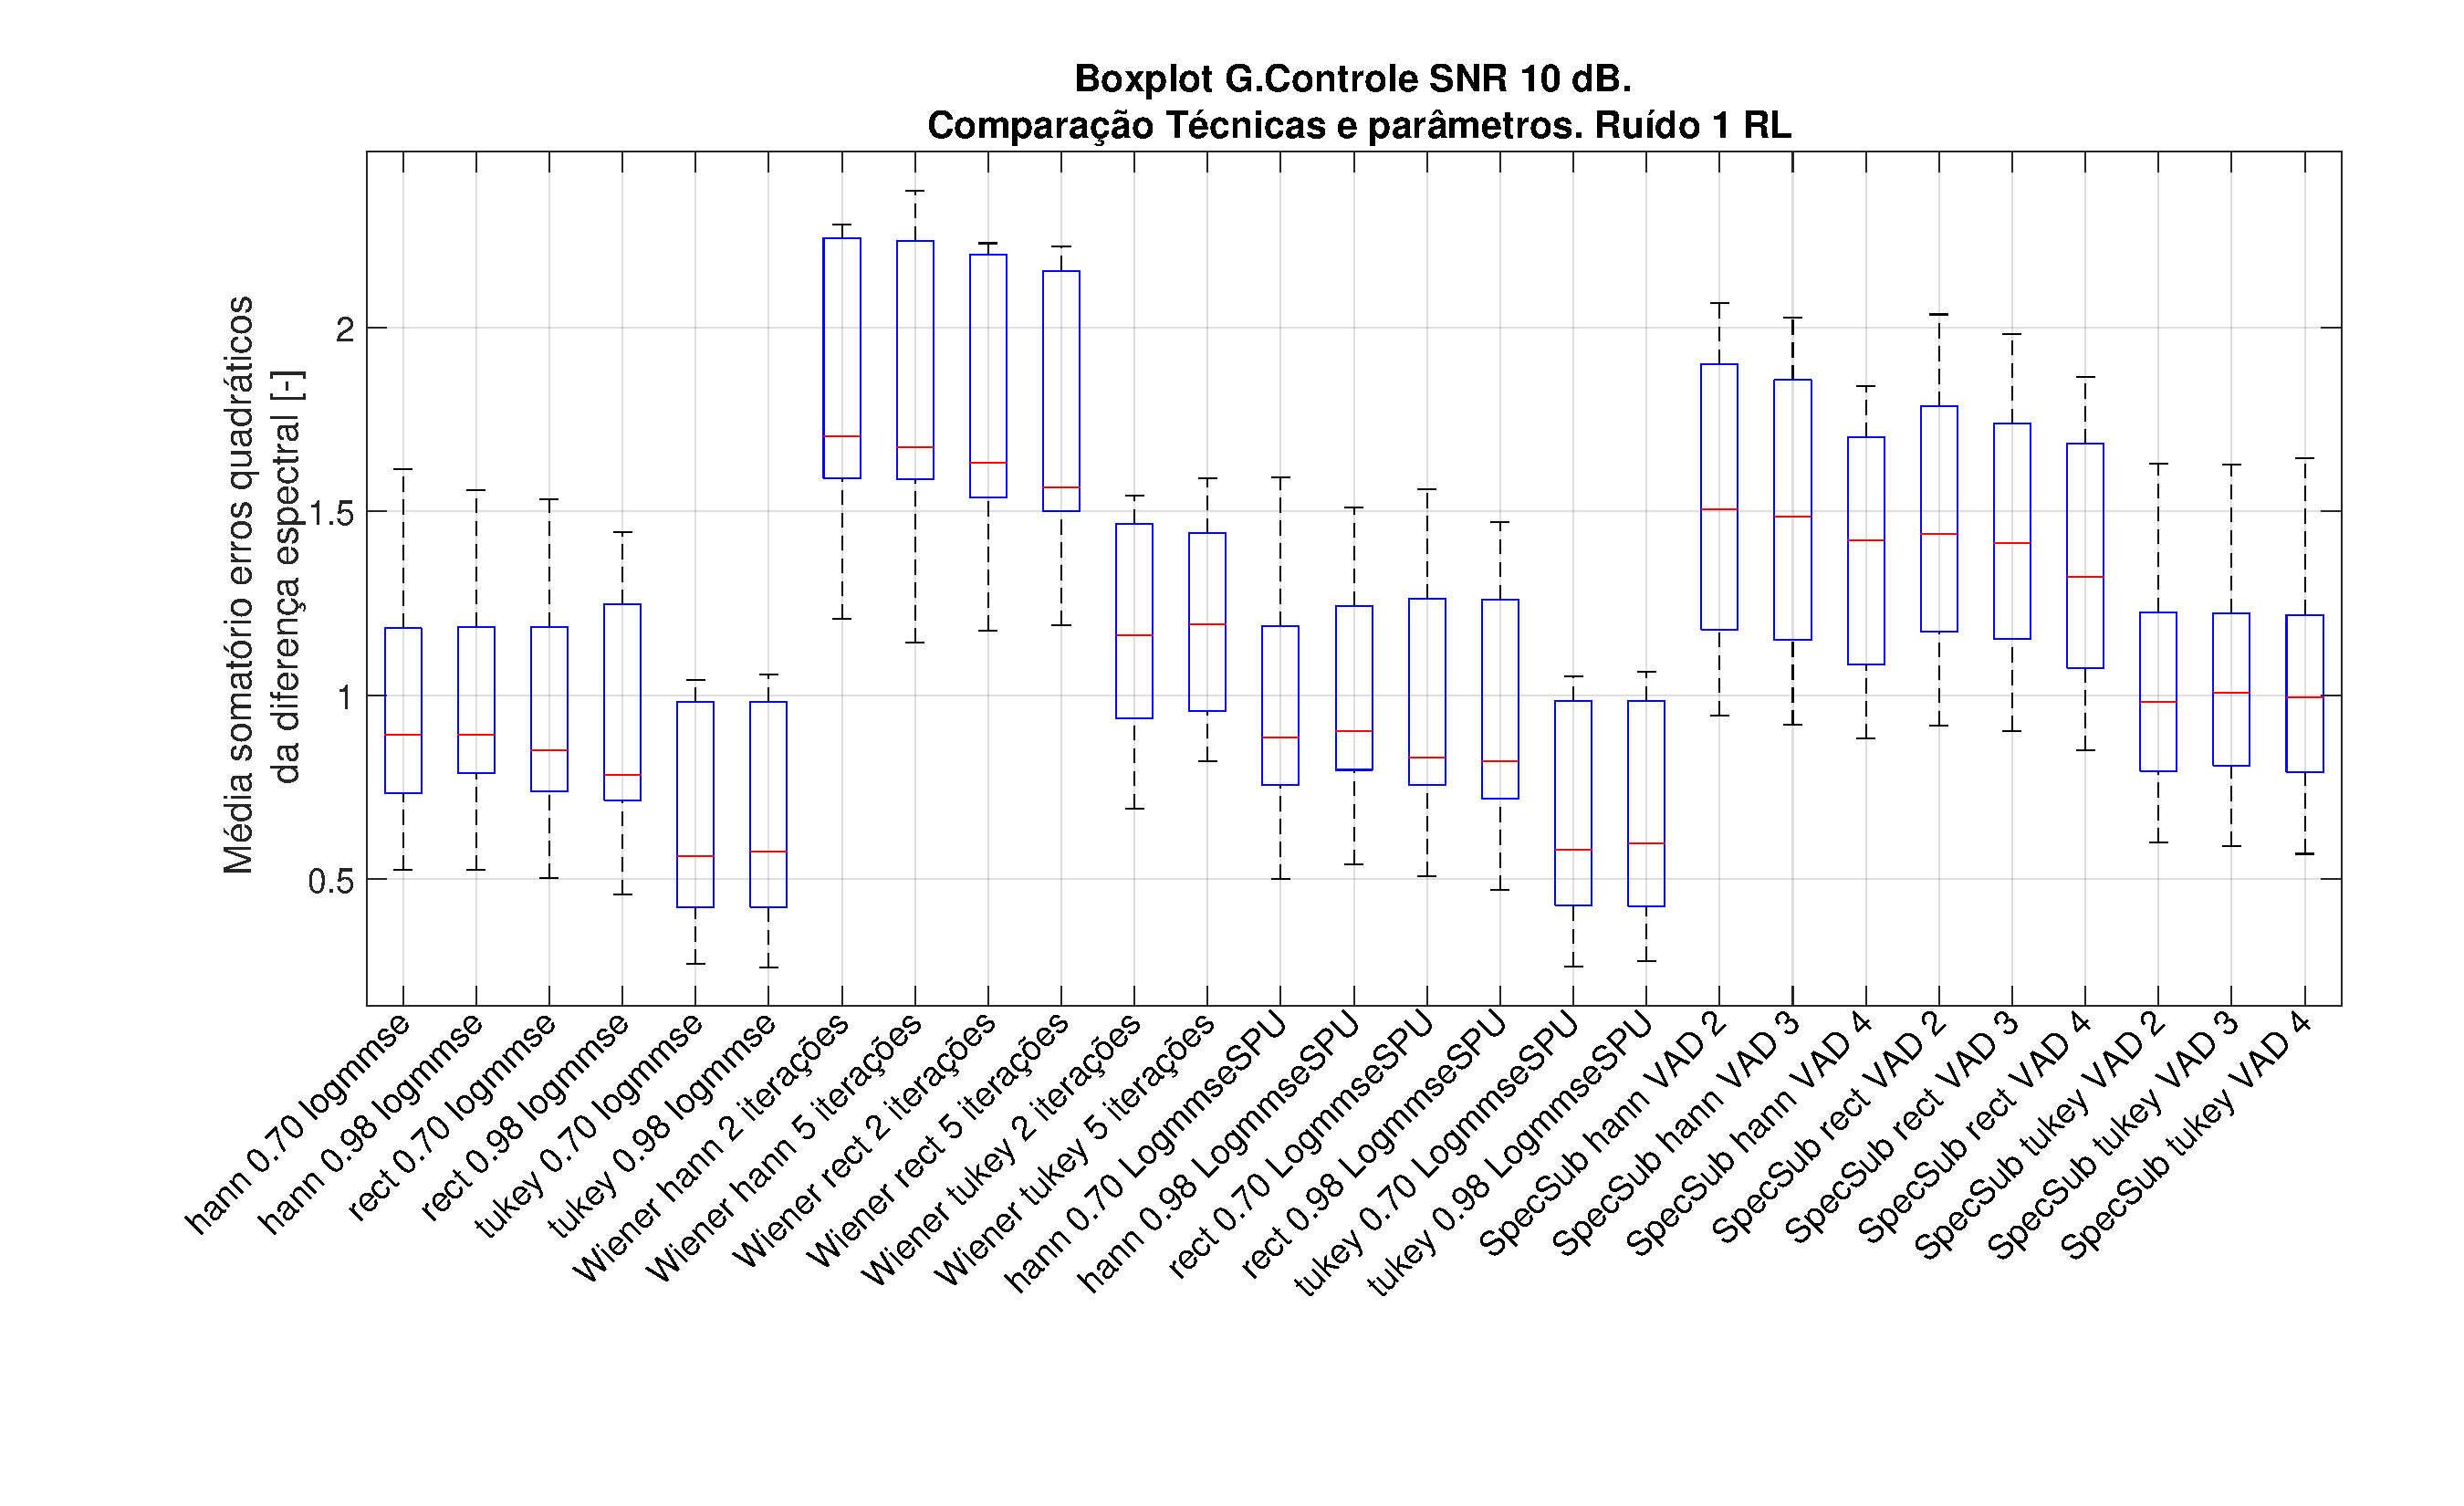
\includegraphics[width=16cm]{Figs/Erro_10_Ruido1.pdf}
\caption{SNR 10 dB Ruído: Restaurant Large.}
\label{snr10_1}
\end{figure}

As \figuras{snr10_2} e \ref{snr10_3} apresentam as mesmas variáveis, contudo para o ruído contaminante RM e RMX respectivamente.

\begin{figure}[H]
\centering
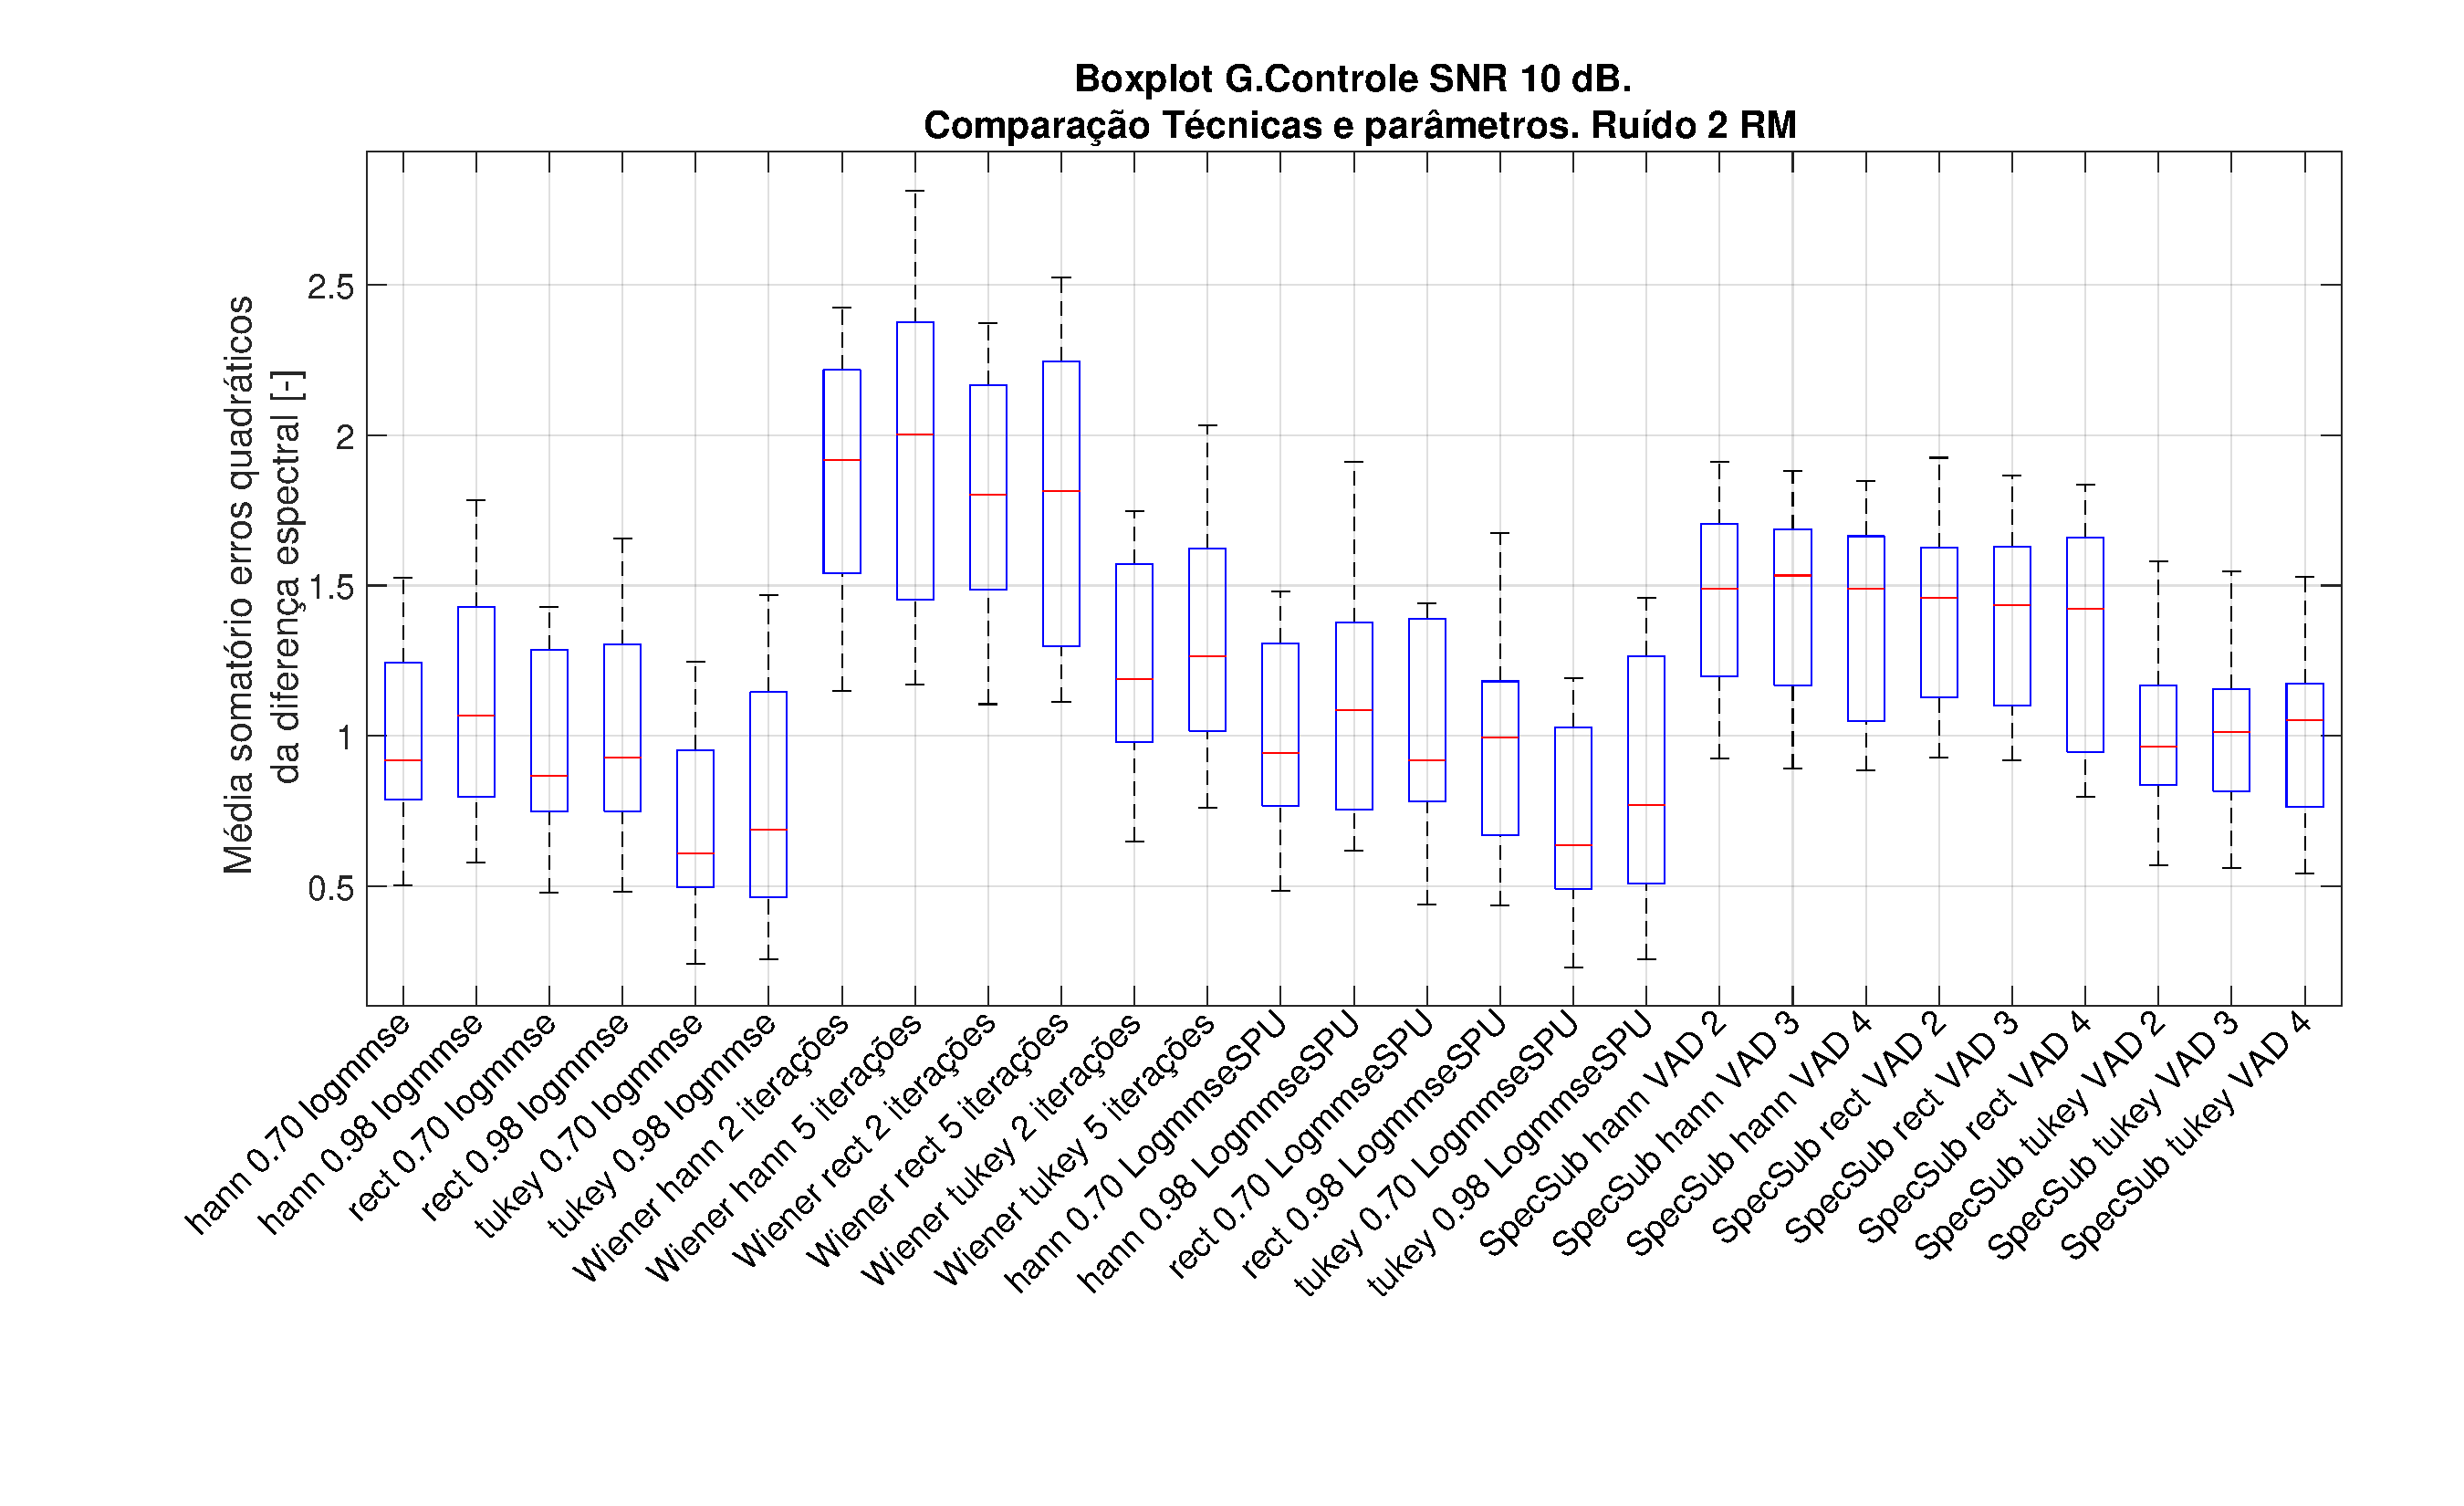
\includegraphics[width=16cm]{Figs/Erro_10_Ruido2.pdf}
\caption{SNR 10 dB Ruído: Restaurant medium.}
\label{snr10_2}
\end{figure}

\begin{figure}[H]
\centering
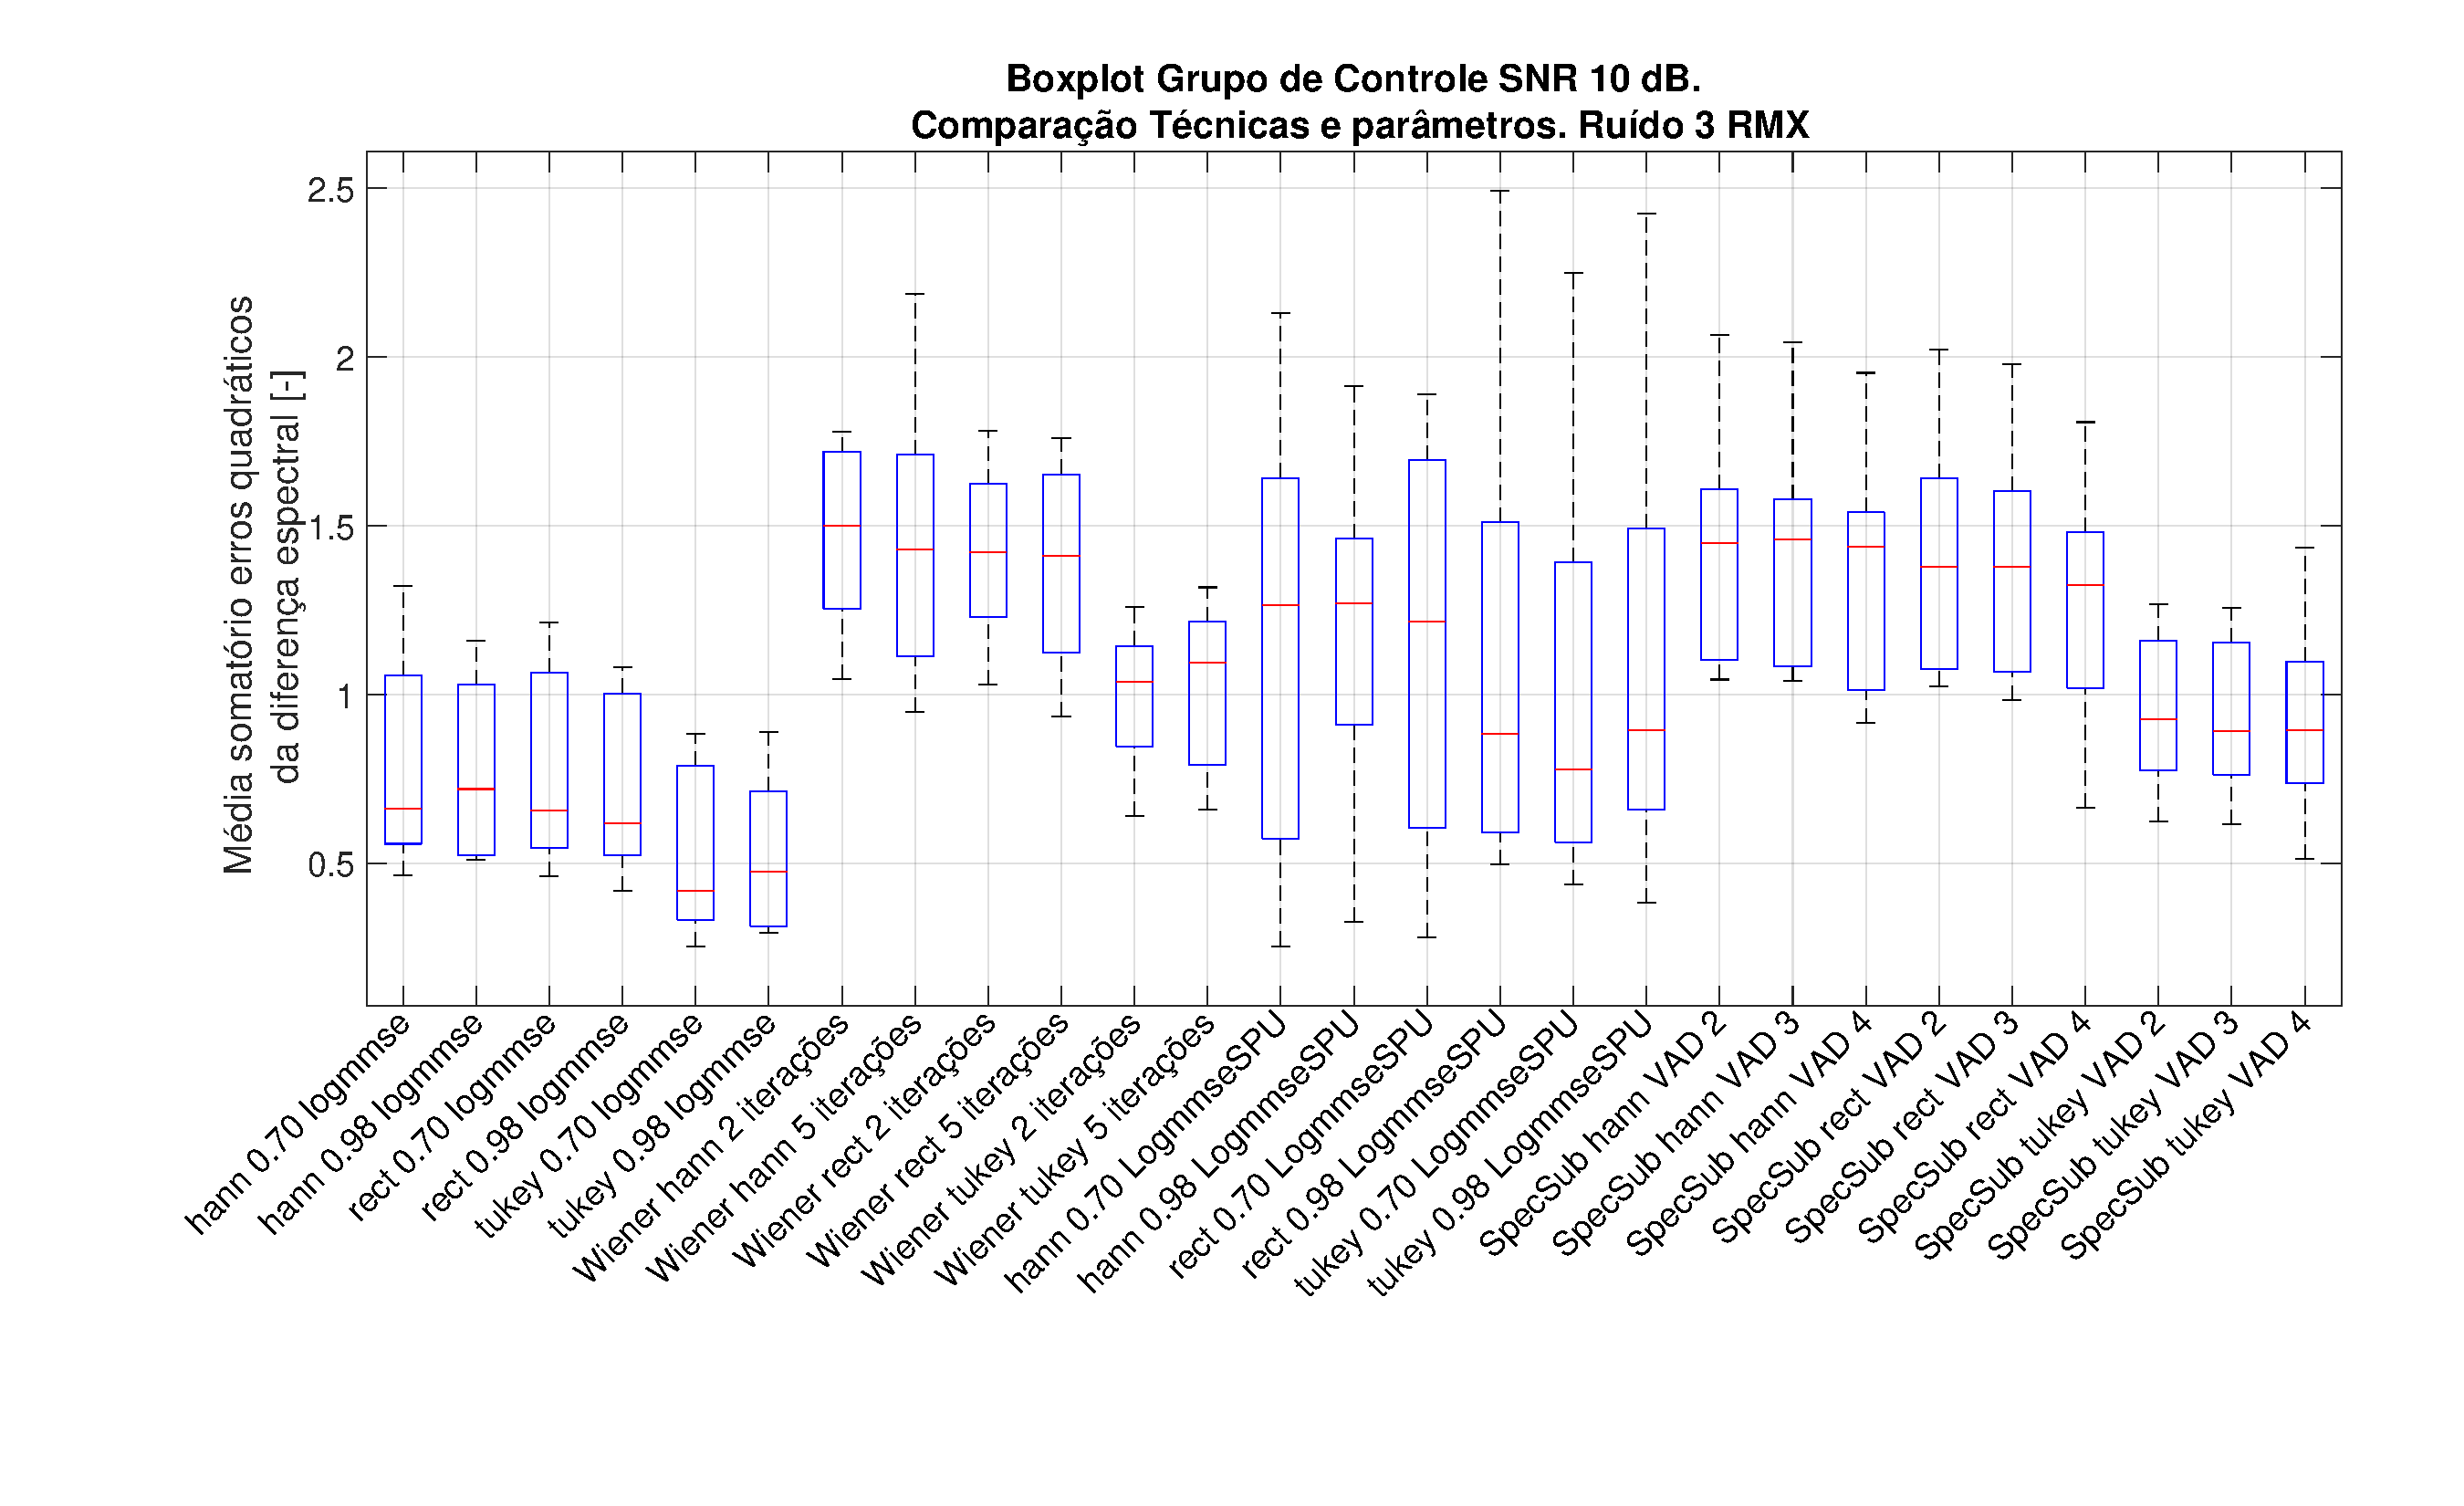
\includegraphics[width=16cm]{Figs/Erro_10_Ruido3.pdf}
\caption{SNR 10 dB Ruído: Restaurant Mexico.}
\label{snr10_3}
\end{figure}

Com a relação sinal ruído bastante elevada os algoritmos Logmmse, filtragem Wiener e subtração espectral apresentaram pouca variação entre os tipos de ruído. Para a técnica Logmmse SPU as medianas dos erros médios quadráticos também mantiveram-se próximas analisando entre os diferentes ruídos, contudo com uma maior amplitude na dispersão dos dados, o que pode ser efeito da menor característica de estacionaridade do ruído onde a decisão do parâmetro  

\begin{figure}[H]
\centering
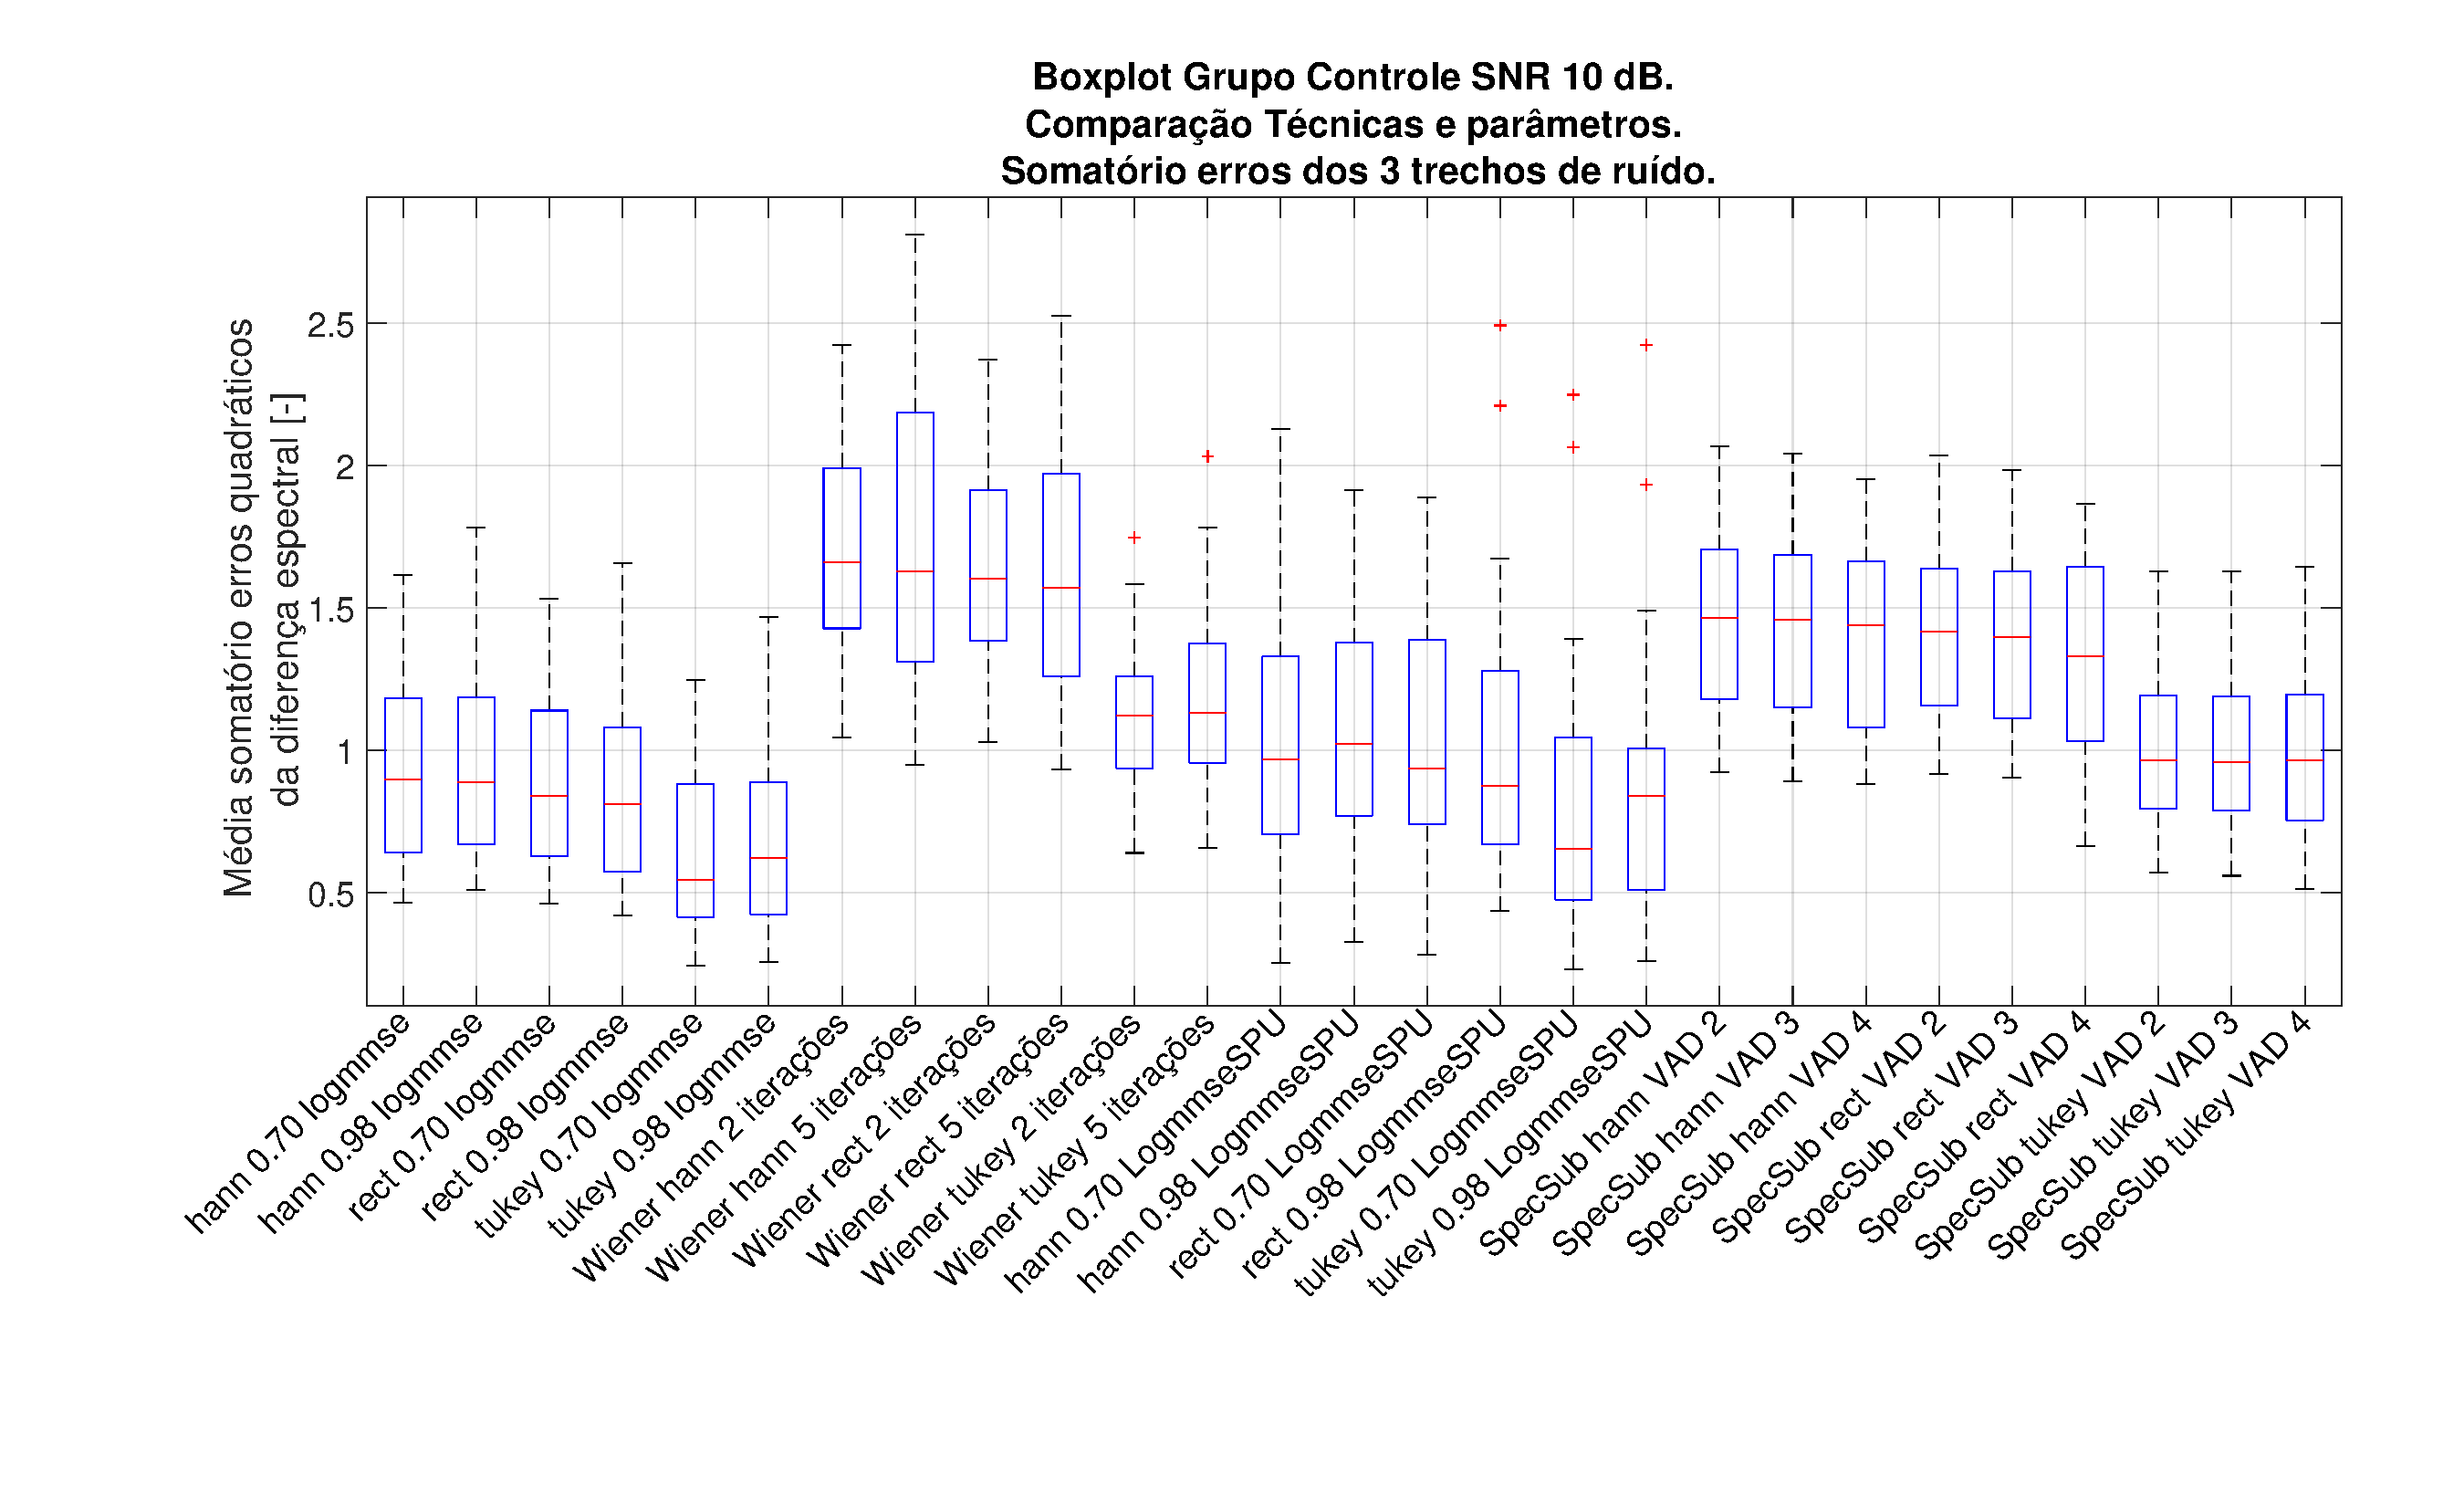
\includegraphics[width=16cm]{Figs/Erro_10_Ruidos.pdf}
\caption{Erro SNR 10 dB todos os ruídos.}
\label{snr10_3r}
\end{figure}

A \figura{snr10_3r} apresenta o erro médio quadrático observando todos os três tipos de ruído apresentados para a alta relação sinal ruído (10~dB). Como houve pouca variação para a mediana de cada técnica\footnote{Para cada técnica houve a aplicação de cada parâmetro selecionado.} entre os ruídos as medianas do conjunto com os três ruídos tem uma maior representação, ocasionando uma melhor decisão dos parâmetros de cada uma para esse caso.




% % Please add the following required packages to your document preamble:
% % \usepackage{graphicx}
% % \usepackage[table,xcdraw]{xcolor}
% % If you use beamer only pass "xcolor=table" option, i.e. \documentclass[xcolor=table]{beamer}
% \begin{table}[]
% \centering
% \caption{My caption}
% \label{my-label}
% \resizebox{\textwidth}{!}{%
% \begin{tabular}{cccc}
% \rowcolor[HTML]{FFFFC7} 
% \multicolumn{4}{c}{\cellcolor[HTML]{FFFFC7}Mediana da somatória dos erros quadráticos da diferença espectral SNR = 10 dB}                                                                                                                                                                                             \\
% \rowcolor[HTML]{ECF4FF} 
% \begin{tabular}[c]{@{}c@{}}Ruído 1 \\ Babbel noise + música\end{tabular}    & \begin{tabular}[c]{@{}c@{}}Ruído 2 \\ Babbel noise\end{tabular}             & \begin{tabular}[c]{@{}c@{}}Ruído 3 \\ Música pronunciada\end{tabular}       & Ruídos combinados                                                           \\
% \rowcolor[HTML]{FFCCC9} 
% \begin{tabular}[c]{@{}c@{}}Wienner Han 2 iter\\ Valor = 1,7005\end{tabular} & \begin{tabular}[c]{@{}c@{}}Wienner Han 5 iter\\ Valor = 2,0015\end{tabular} & \begin{tabular}[c]{@{}c@{}}SpecSub Han VAD 3 \\ Valor = 1,4580\end{tabular} & \begin{tabular}[c]{@{}c@{}}Wiener Han 2 iter\\ Valor = 1,662\end{tabular}   \\
% \rowcolor[HTML]{ECF4FF} 
% \begin{tabular}[c]{@{}c@{}}Logmmse Tukey 0,70\\ Valor = 0,5614\end{tabular} & \begin{tabular}[c]{@{}c@{}}Logmmse Tukey 0,70\\ Valor = 0,6101\end{tabular} & \begin{tabular}[c]{@{}c@{}}Logmmse Tukey 0,70\\ Valor = 0,4173\end{tabular} & \begin{tabular}[c]{@{}c@{}}Logmmse Tukey 0,70\\ Valor = 0,5459\end{tabular}
% \end{tabular}%
% }
% \end{table}


A \tabela{tabelaGeral} apresenta os melhores e piores valores de mediana para cada relação sinal ruído considerando cada ruído diferente e o valor combinado relativo a amostragem com os três ruídos. 

\begin{table}[H]
\centering
\caption{Valores de mediana para o somatória dos erros quadráticos médios da diferença espectral entre sinal processado e sinal original.}
\label{tabelaGeral}
\resizebox{\textwidth}{!}{%
\begin{tabular}{lcccc}
\rowcolor[HTML]{EFF1FF} & \multicolumn{4}{c}{Mediana da somatória dos erros quadráticos da diferença espectral  Tabela Geral} \\
\rowcolor[HTML]{EFF1FF} & \begin{tabular}[c]{@{}c@{}}Ruído 1 \\ Babbel noise + música\end{tabular} & \begin{tabular}[c]{@{}c@{}}Ruído 2 \\ Babbel noise\end{tabular} & \begin{tabular}[c]{@{}c@{}}Ruído 3 \\ Música pronunciada\end{tabular} & Ruídos combinados \\
 
\rowcolor[HTML]{FFCCC9} SNR = -10 dB & \begin{tabular}[c]{@{}c@{}}Logmmse Han 0,70\\ Valor = 2,987\end{tabular} & \begin{tabular}[c]{@{}c@{}}Logmmse Rect 0,70\\ Valor = 2,1803\end{tabular} & \begin{tabular}[c]{@{}c@{}}SpecSub Rect VAD 2 \\ Valor = 1,5300\end{tabular} & \begin{tabular}[c]{@{}c@{}}Logmmse Rect 0,70\\ Valor = 2,1372\end{tabular} \\
SNR = -10 dB & \begin{tabular}[c]{@{}c@{}}SpecSub Tukey VAD 4\\ Valor = 1,1683\end{tabular} & \begin{tabular}[c]{@{}c@{}}Logmmse SPU Rect 0,98\\ Valor = 0,7169\end{tabular} & \begin{tabular}[c]{@{}c@{}}Logmmse Tukey 0,98\\ Valor = 0,26817\end{tabular} & \begin{tabular}[c]{@{}c@{}}Logmmse Hann 0,98\\ Valor = 0,9965\end{tabular} \\
\rowcolor[HTML]{FFCCC9} SNR = 0 dB & \begin{tabular}[c]{@{}c@{}}Wienner Han 5 iter\\ Valor = 2,0464\end{tabular} & \begin{tabular}[c]{@{}c@{}}Wienner Han 2 iter\\ Valor = 1,7176\end{tabular}  & \begin{tabular}[c]{@{}c@{}}Logmmse SPU Tukey 0,98\\ Valor = 1,3208\end{tabular} & \begin{tabular}[c]{@{}c@{}}Wienner Han 5 iter\\ Valor = 1,5205\end{tabular} \\
SNR = 0 dB & \begin{tabular}[c]{@{}c@{}}SpecSub Rect VAD 4\\ Valor = 0,8156\end{tabular} & \begin{tabular}[c]{@{}c@{}}SpecSub Tukey VAD 4\\ Valor = 0,8138\end{tabular} & \begin{tabular}[c]{@{}c@{}}Wienner Tukey 5 iter\\ Valor = 0,4994\end{tabular}   & \begin{tabular}[c]{@{}c@{}}SpecSub Tukey VAD 4\\ Valor = 0,8018\end{tabular} \\
\rowcolor[HTML]{FFCCC9}SNR = 10 dB & \begin{tabular}[c]{@{}c@{}}Wienner Han 2 iter\\ Valor = 1,7005\end{tabular} & \begin{tabular}[c]{@{}c@{}}Wienner Han 5 iter\\ Valor = 2,0015\end{tabular} & \begin{tabular}[c]{@{}c@{}}SpecSub Han VAD 3 \\ Valor = 1,4580\end{tabular} & \begin{tabular}[c]{@{}c@{}}Wiener Han 2 iter\\ Valor = 1,662\end{tabular} \\
SNR = 10 dB & \begin{tabular}[c]{@{}c@{}}Logmmse Tukey 0,70\\ Valor = 0,5614\end{tabular} & \begin{tabular}[c]{@{}c@{}}Logmmse Tukey 0,70\\ Valor = 0,6101\end{tabular} & \begin{tabular}[c]{@{}c@{}}Logmmse Tukey 0,70\\ Valor = 0,4173\end{tabular} & \begin{tabular}[c]{@{}c@{}}Logmmse Tukey 0,70\\ Valor = 0,5459\end{tabular}\\
\end{tabular}%
}
\end{table}

É possível notar que para uma SNR a melhor combinação de técnica e parâmetro para obtenção de um erro médio quadrático baixo nem sempre é a mesma entre os diferentes tipos de ruído, assim quando combinados os ruídos e tendo uma avaliação sob essa combinação a escolha apresenta um compromisso, buscando acertar mais quantidade de processos próximos ao valor da mediana da combinação do que valores absolutos de alguma combinação para um ruído específico. Isso é relevante a medida que tem-se diferentes ruídos ou ruídos intermitentes ou de bastante variação. 


A partir da quantificação dos erros quadráticos médios de cada relação sinal ruído (-10~dB, 0~dB e 10~dB) de cada técnica, foram selecionados e apresentados na \tabela{Final1} os parâmetros com melhor desempenho.

\begin{table}[H]
\centering
\caption{Parâmetros Selecionados}
\label{Final1}
%\resizebox{\textwidth}{!}{%
\begin{tabular}{cccc}
%\multicolumn{1}{l}{} & \multicolumn{3}{c}{SNR} \\
\multicolumn{1}{l}{\multirow{-2}{*}{}} & \cellcolor[HTML]{FFFFFF}-10 dB & \cellcolor[HTML]{FFFFFF}0 dB & \cellcolor[HTML]{FFFFFF}10 dB \\
\rowcolor[HTML]{FFCCC9} 
SpecSub & \begin{tabular}[c]{@{}c@{}}Janela Hanning\\ VAD = 4 dB\end{tabular} & \begin{tabular}[c]{@{}c@{}}Janela Tukey\\ VAD = 4 dB\end{tabular} & \begin{tabular}[c]{@{}c@{}}Janela Tukey\\ VAD = 4 dB\end{tabular} \\
\rowcolor[HTML]{FFFFC7} 
Wiener & \begin{tabular}[c]{@{}c@{}}Janela Tukey\\ 2 iterações\end{tabular} & \begin{tabular}[c]{@{}c@{}}Janela Tukey\\ 5 iterações\end{tabular} & \begin{tabular}[c]{@{}c@{}}Janela Tukey\\ 5 iterações\end{tabular} \\
\rowcolor[HTML]{FFCCC9} 
Logmmse & \begin{tabular}[c]{@{}c@{}}Janela Hanning\\ $\alpha$ = 0,98\end{tabular} & \begin{tabular}[c]{@{}c@{}}Janela Tukey\\ $\alpha$ = 0,98\end{tabular} & \begin{tabular}[c]{@{}c@{}}Janela Tukey\\ $\alpha$ = 0,70\end{tabular} \\
\rowcolor[HTML]{FFFFC7} 
Logmmse SPU & \begin{tabular}[c]{@{}c@{}}Janela Tukey\\ $\alpha$ = 0,98\end{tabular} & \begin{tabular}[c]{@{}c@{}}Janela Retangular\\ $\alpha$ = 0,98\end{tabular} & \begin{tabular}[c]{@{}c@{}}Janela Tukey\\ $\alpha$ = 0,70\end{tabular}
\end{tabular}%
%}
\end{table}
    
A definição dos parâmetros variou também conforme a SNR, dado que as técnicas e os parâmetros agem de formas diferentes em SNR diferentes , por exemplo, o número de iterações na técnica de filtragem Wiener adaptativa, onde há uma redução do erro médio quadrático ao aumentar o número de iterações em SNR altas, apesar da magnitude do erro crescer dada a característica da técnica não ser a mais adequada à altas SNR.

Assim a decisão dos parâmetros fixos infere na obtenção de resultados de erro quadrático médio não otimizados e uma consequente eficiência da técnica prejudicada em alguns casos, contudo na expectativa de acertar a maior parte dos casos. 




% \subsection{Resultados subjetivos Grupo de controle}

% Para a análise subjetiva foram selecionados áudios do grupo de controle a partir dos resultados objetivos e apresentados na \tabela{tabelafim}. 

% Técnicas e parâmetros discrepantes selecionados:

% % % Please add the following required packages to your document preamble:
% % % \usepackage{graphicx}
% % % \usepackage[table,xcdraw]{xcolor}
% % % If you use beamer only pass "xcolor=table" option, i.e. \documentclass[xcolor=table]{beamer}
% % \begin{table}[H]
% % \centering
% % \caption{Técnicas e parâmetros selecionados pela discrepância da mediana do erro médio quadrático da diferença espectral selecionados para avaliação subjetiva por diferentes SNR.}
% % \label{tabelafim}
% % \resizebox{\textwidth}{!}{%
% % \begin{tabular}{cccc}
% % \rowcolor[HTML]{FFCCC9} 
% % \cellcolor[HTML]{FFFFFF} & &\multicolumn{3}{c}{\cellcolor[HTML]{FFCCC9}Mediana da somatória dos erros quadráticos da diferença espectral  Tabela Geral} \\
% % \rowcolor[HTML]{96FFFB} 
% % SNR [dB] & \begin{tabular}[c]{@{}c@{}}Ruído 1 \\ Babbel noise + música\end{tabular} & \begin{tabular}[c]{@{}c@{}}Ruído 2 \\ Babbel noise\end{tabular} & \begin{tabular}[c]{@{}c@{}}Ruído 3 \\ Música pronunciada\end{tabular} \\
% % \rowcolor[HTML]{ECF4FF} 
% % -10 & \begin{tabular}[c]{@{}c@{}}Logmmse \\Janela Hanning $\alpha = 0,70$ \\ \textit{vs} \\ Subtração Espectral \\ Janela Retangular VAD 4 dB\end{tabular} & \begin{tabular}[c]{@{}c@{}}Logmmse \\Janela Retangular $\alpha = 0,70$ \\ \textit{vs}\\  Logmmse SPU \\Retangular $\alpha = 0,98$\end{tabular} & \begin{tabular}[c]{@{}c@{}}Subtração Espectral\\ Retangular VAD 2\\ \textit{vs}\\ Logmmse\\ Tukey $\alpha = 0,98$\end{tabular} \\
% % \rowcolor[HTML]{FFFC9E} 
% % 0 & \begin{tabular}[c]{@{}c@{}}Wienner \\Han 5 iter\\ \textit{vs}\\ Subtração Espectral \\ Retangular VAD 4\end{tabular} & \begin{tabular}[c]{@{}c@{}}Wienner \\ Han 2 iter\\ \textit{vs}\\ Subtração Espectral \\Tukey VAD 4\end{tabular} & \begin{tabular}[c]{@{}c@{}}Logmmse SPU \\ Retangular $\alpha = 0,98$\\ \textit{vs}\\ Wienner \\ Tukey 5 iter\end{tabular} \\
% % \rowcolor[HTML]{ECF4FF} 
% % 10 & \begin{tabular}[c]{@{}c@{}}Wienner \\ Han 2 iter\\ \textit{vs}\\ Logmmse \\ Tukey $\alpha = 0,70$\end{tabular} & \begin{tabular}[c]{@{}c@{}}Wienner Han 5 iter\\ \textit{vs}\\ Logmmse \\ Tukey $\alpha = 0,70$\end{tabular} & \begin{tabular}[c]{@{}c@{}}Subtração Espectral \\ Retangular VAD 2\\ \textit{vs}\\ Logmmse \\ Tukey $\alpha = 0,70$\end{tabular} & \begin{tabular}[c]{@{}c@{}}Wienner Han 2 iter\\ \textit{vs}\\ Logmmse \\ Tukey $\alpha = 0,70$\end{tabular}
% % \end{tabular}%
% % }
% % \end{table}

% Por conveniência foram apresentados os sinais relativos a 1~frase (18~sinais ao todo). O teste subjetivo interno foi realizado com alunos da disciplina apenas a título de demonstração, demorou em média 8 minutos e apontou a preferência apresentada na \tabela{} em uma escala de 1~a~5 na comparação pareada sem tempo de recursão dado a pequena duração do sinal. 

% Foram selecionados as técnicas com os parâmetros que apresentaram:

% \begin{enumerate}[label=(\roman*)]
%     \item Menor e maior  valor de mediana para o somatória dos erros quadráticos da diferença espectral considerando os 3 ruídos 
%     \item Menor e maior  valor de mediana para o somatória dos erros quadráticos da diferença espectral considerando Ruído 1 (RL) 
%     \item Menor e maior  valor de mediana para o somatória dos erros quadráticos da diferença espectral considerando Ruído 2 (RM)
%     \item Menor e maior valor de mediana para o somatória dos erros quadráticos da diferença espectral considerando Ruído 3 (RMX)
% \end{enumerate}

% O intuito é avaliar relação da representatividade da qualidade sonora subjetiva através da média dos erros quadráticos da diferença espectral.

% O sinal de fala foi aleatoriamente selecionado dentro do conjunto dos 10 sinais de fala do grupo de controle. Para as comparações das diferentes SNR com a variação de técnicas para o ruído 1 (RL), foi selecionado a fala 1, referente ao arquivo \textbf{F130101.WAV}, para o ruído 2~(RM) foi selecionado a fala 2 referente ao arquivo \textbf{F130102.WAV} e para o ruído 3 a fala 3 referente ao arquivo \textbf{F130103.WAV}.

% Para as médias de combinação dos ruídos contaminada com os três ruídos.



\subsection{Parâmetros escolhidos para técnicas a partir dos resultados do Grupo de controle}

Os parâmetros de entrada das técnicas que foram variados no grupo de controle e obtiveram menor erro médio quadrático na diferença espectral entre o sinal original e o sinal contaminado e processado individualmente por cada técnica 

Para cada técnica os parâmetros são apresentados na tabela \tabela{Final2}

\begin{table}[H]
\centering
\caption{Parâmetros escolhidos para aplicação nas técnicas de supressão de ruído.}
\label{Final2}
\begin{tabular}{ccc}
\multicolumn{1}{l}{\multirow{-2}{*}{}} & \cellcolor[HTML]{FFFFFF} & \cellcolor[HTML]{FFFFFF} \\
\rowcolor[HTML]{FFCCC9} 
SpecSub & Tukey & 4 dB \\
\rowcolor[HTML]{FFFFC7} 
Wiener & Tukey & 5 iterações \\
\rowcolor[HTML]{FFCCC9} 
Logmmse & Tukey & $\alpha$ = 0,98 \\
\rowcolor[HTML]{FFFFC7} 
Logmmse SPU & Tukey & $\alpha$ = 0,98
\end{tabular}%
\end{table}
        


\subsection{Análise geral}
\label{secgmaior}

O grupo maior foi composto dos 20 sinais de fala restantes. Tais falas foram contaminadas com 5 trechos diferentes de cada um dos 3 ruídos, 5 SNR diferentes de -10~dB, -5~dB, 0~dB, 5~dB, 10~dB, assim são 1.500 arquivos para cada algoritmo, em um total de 6.000 arquivos analisados.


\begin{figure}[H]
\subfloat[SNR -10 dB.]{\label{tm10}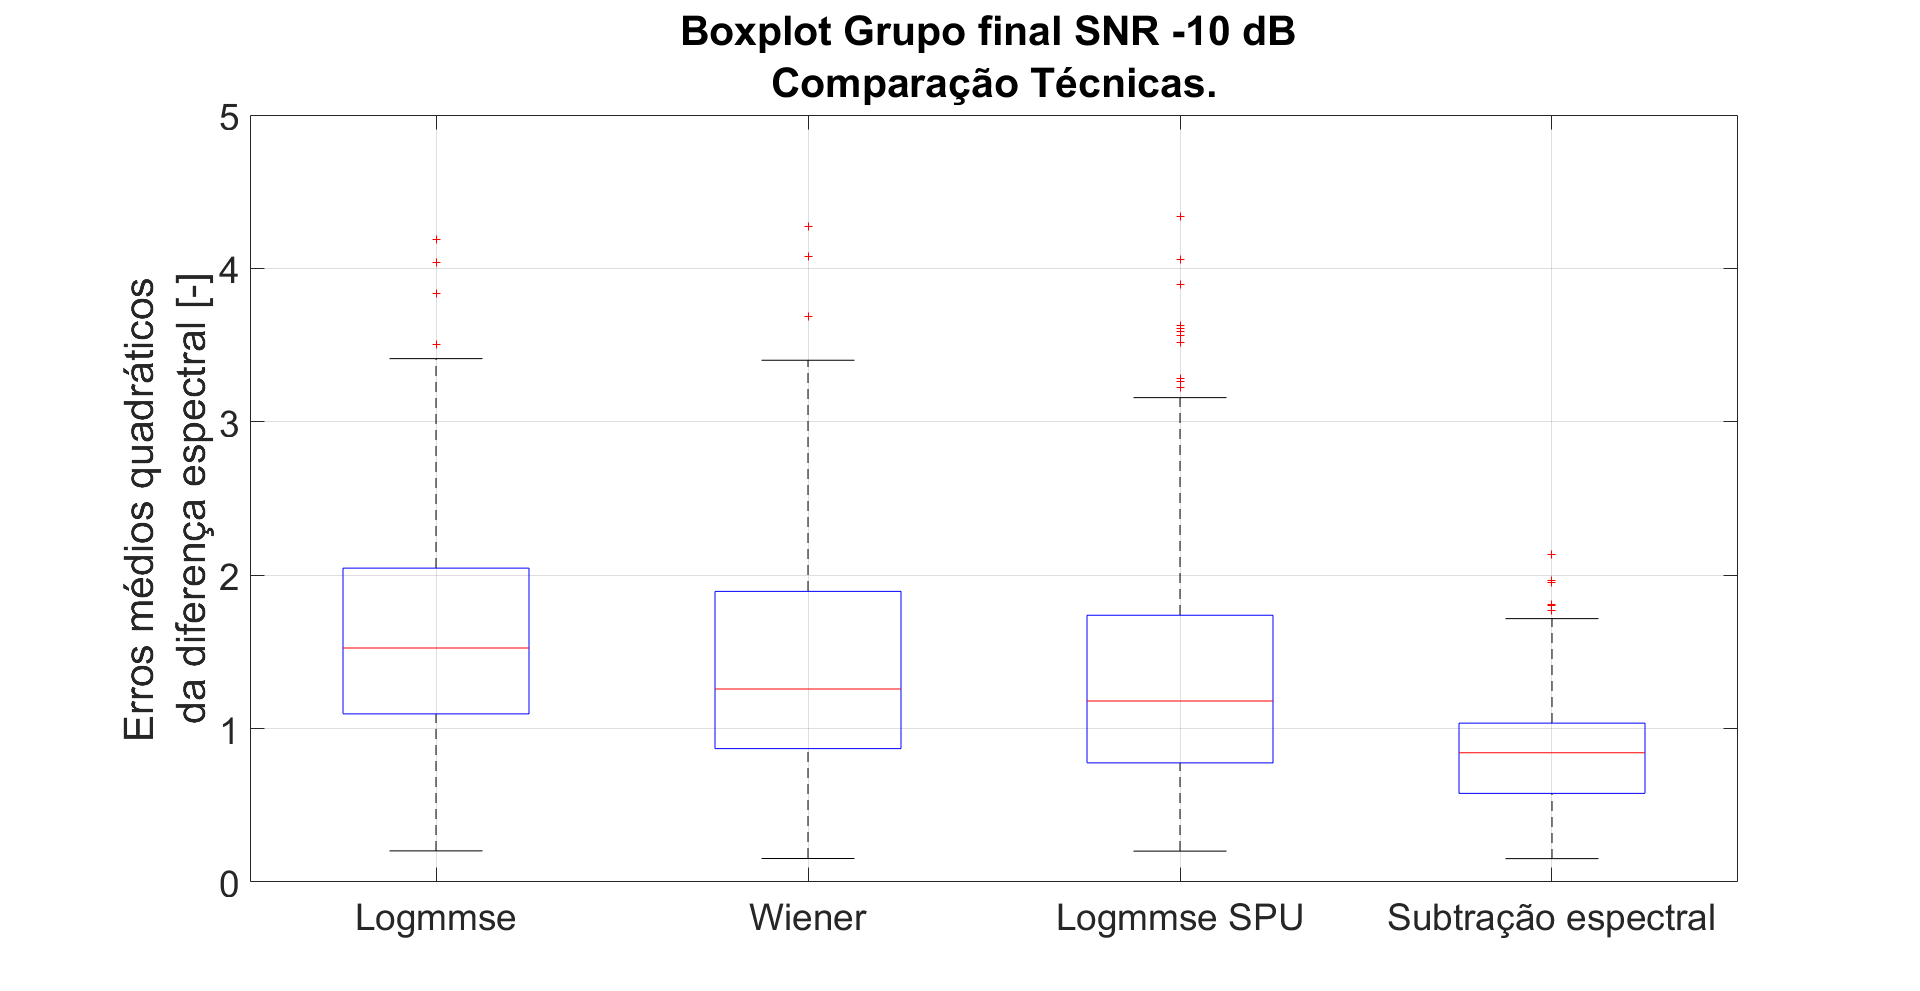
\includegraphics[width=8.5cm,]{Figs/Total_m10a}}\quad
\subfloat[SNR -5 dB.]{\label{tm5}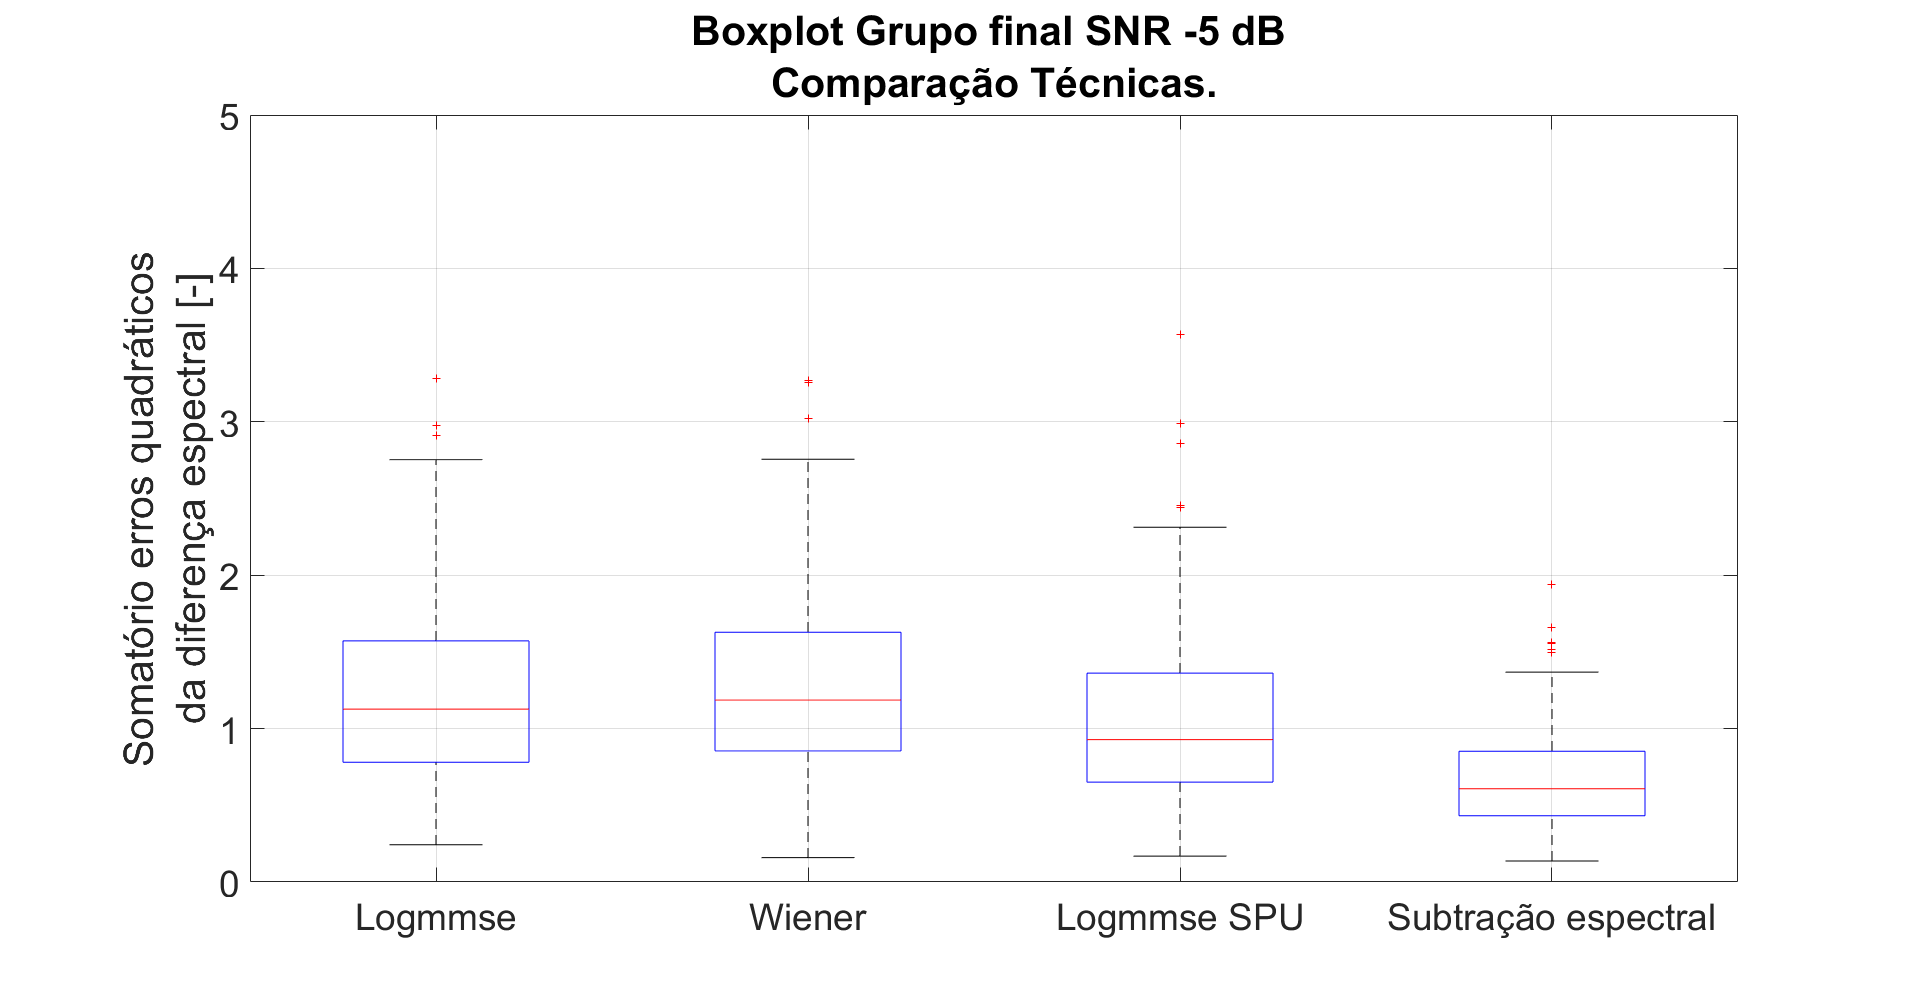
\includegraphics[width=8.5cm,]{Figs/Total_m5a}}
\caption{Erro quadrático médio entre as técnicas de supressão com SNR diferentes.}
\label{aff1}
\end{figure}

\begin{figure}[H]
\subfloat[SNR 0 dB.]{\label{tm101}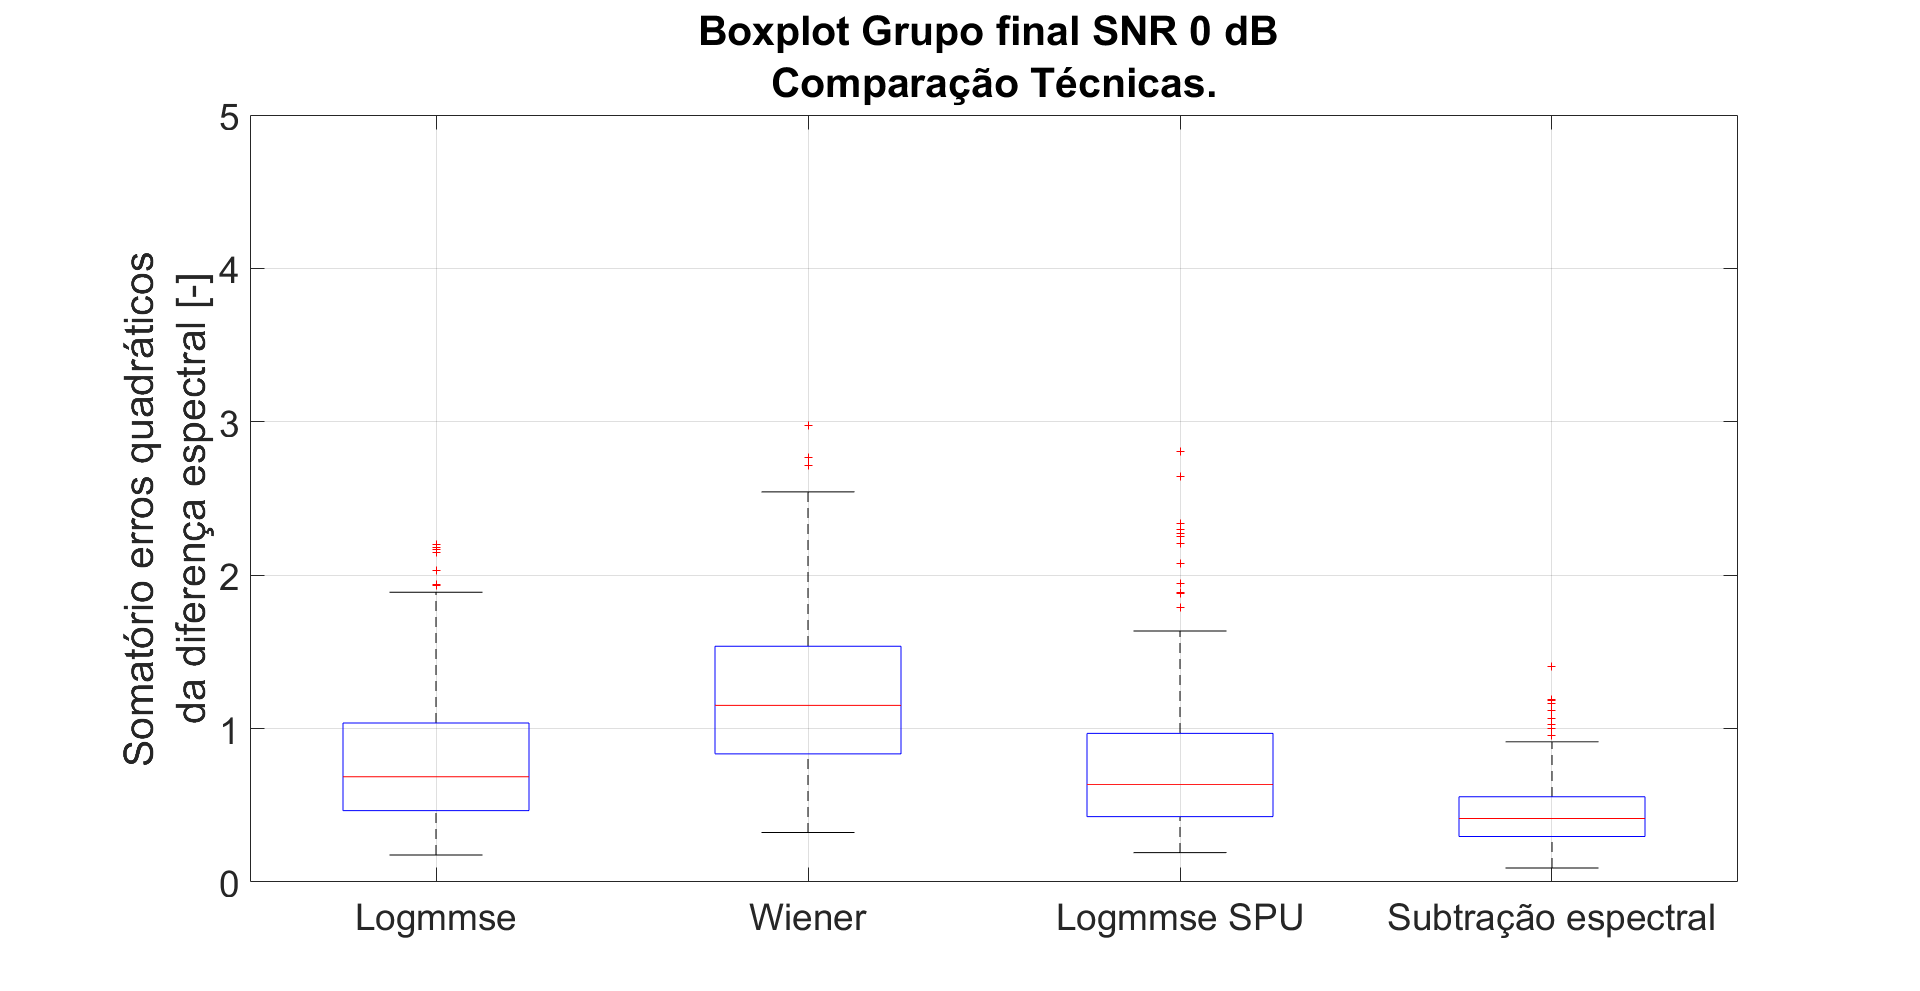
\includegraphics[width=8.5cm,]{Figs/Total_01.png}}\quad
\subfloat[SNR 5 dB.]{\label{tm51}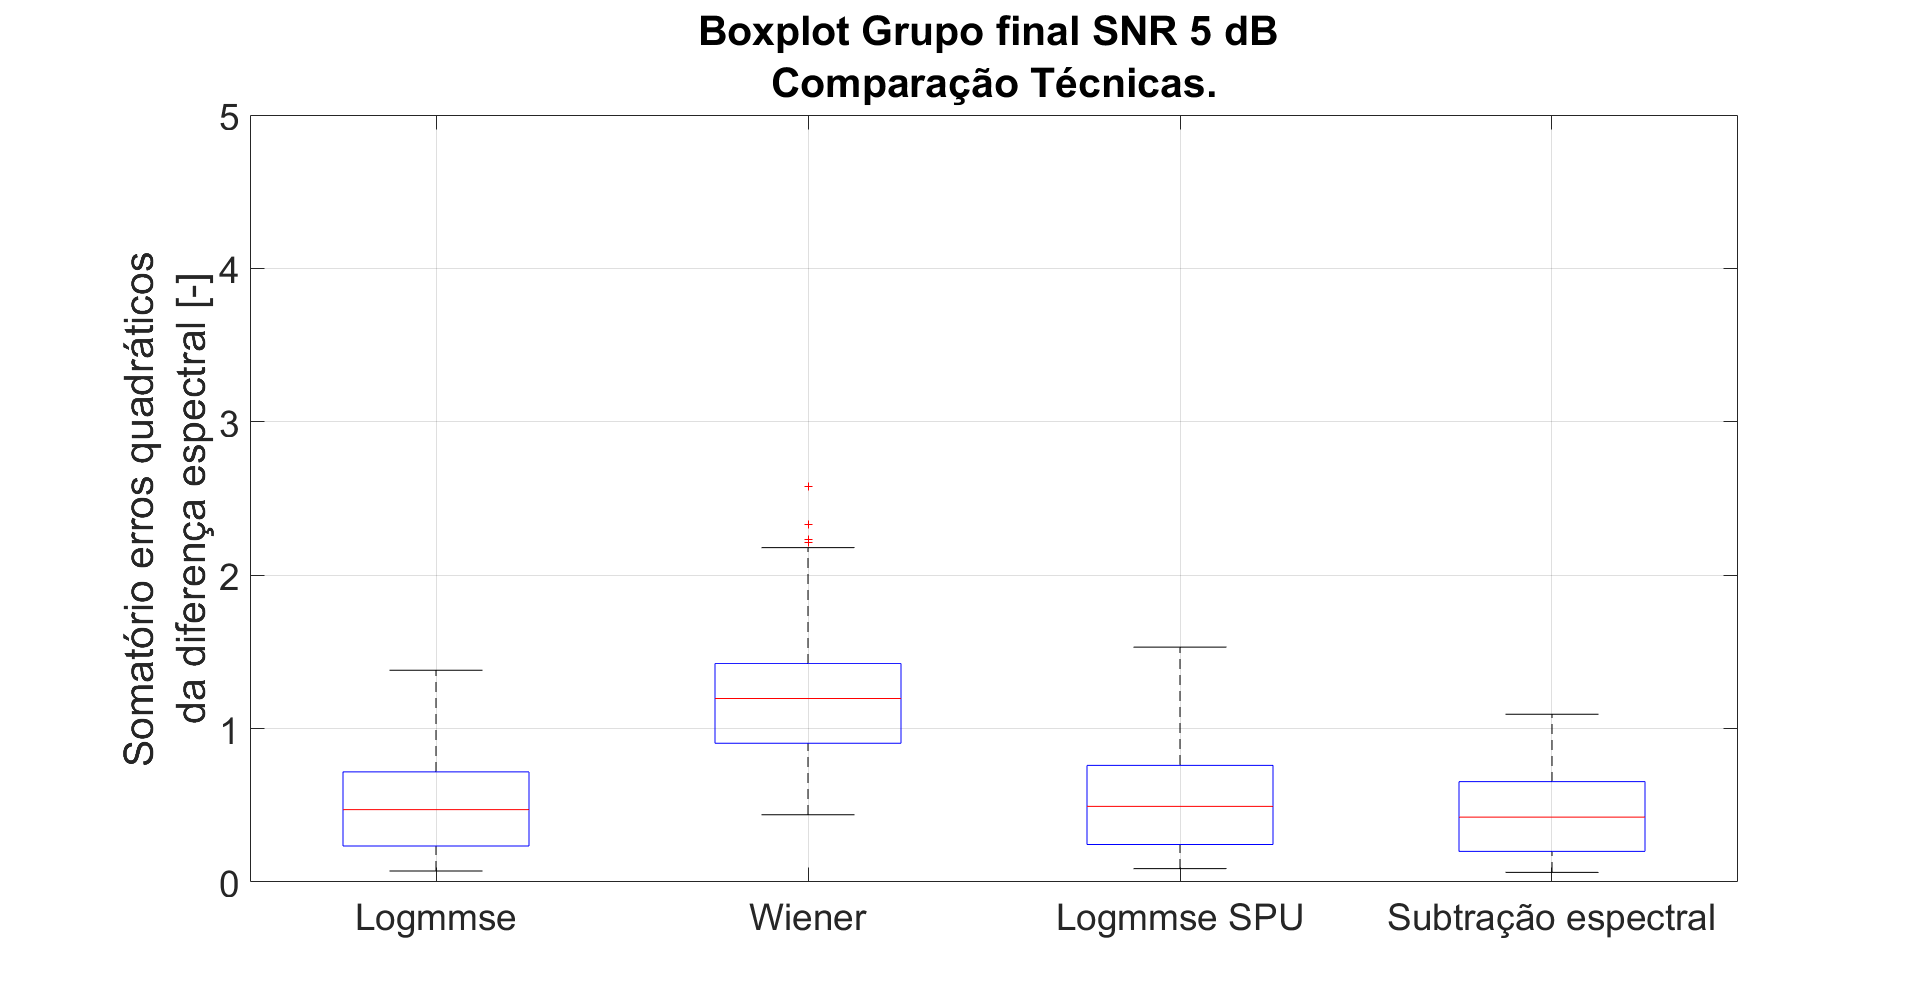
\includegraphics[width=8.5cm,]{Figs/Total_5a}}
\caption{Erro quadrático médio entre as técnicas de supressão com SNR diferentes.}
\label{aff2}
\end{figure}

As \figuras{aff1} \fign{aff2} e \fign {total_m10} apresentam para cada SNR os valores de erro quadrático médio em função da técnica utilizada com os parâmetros obtidos através do grupo de controle.

\begin{figure}[H]
\centering
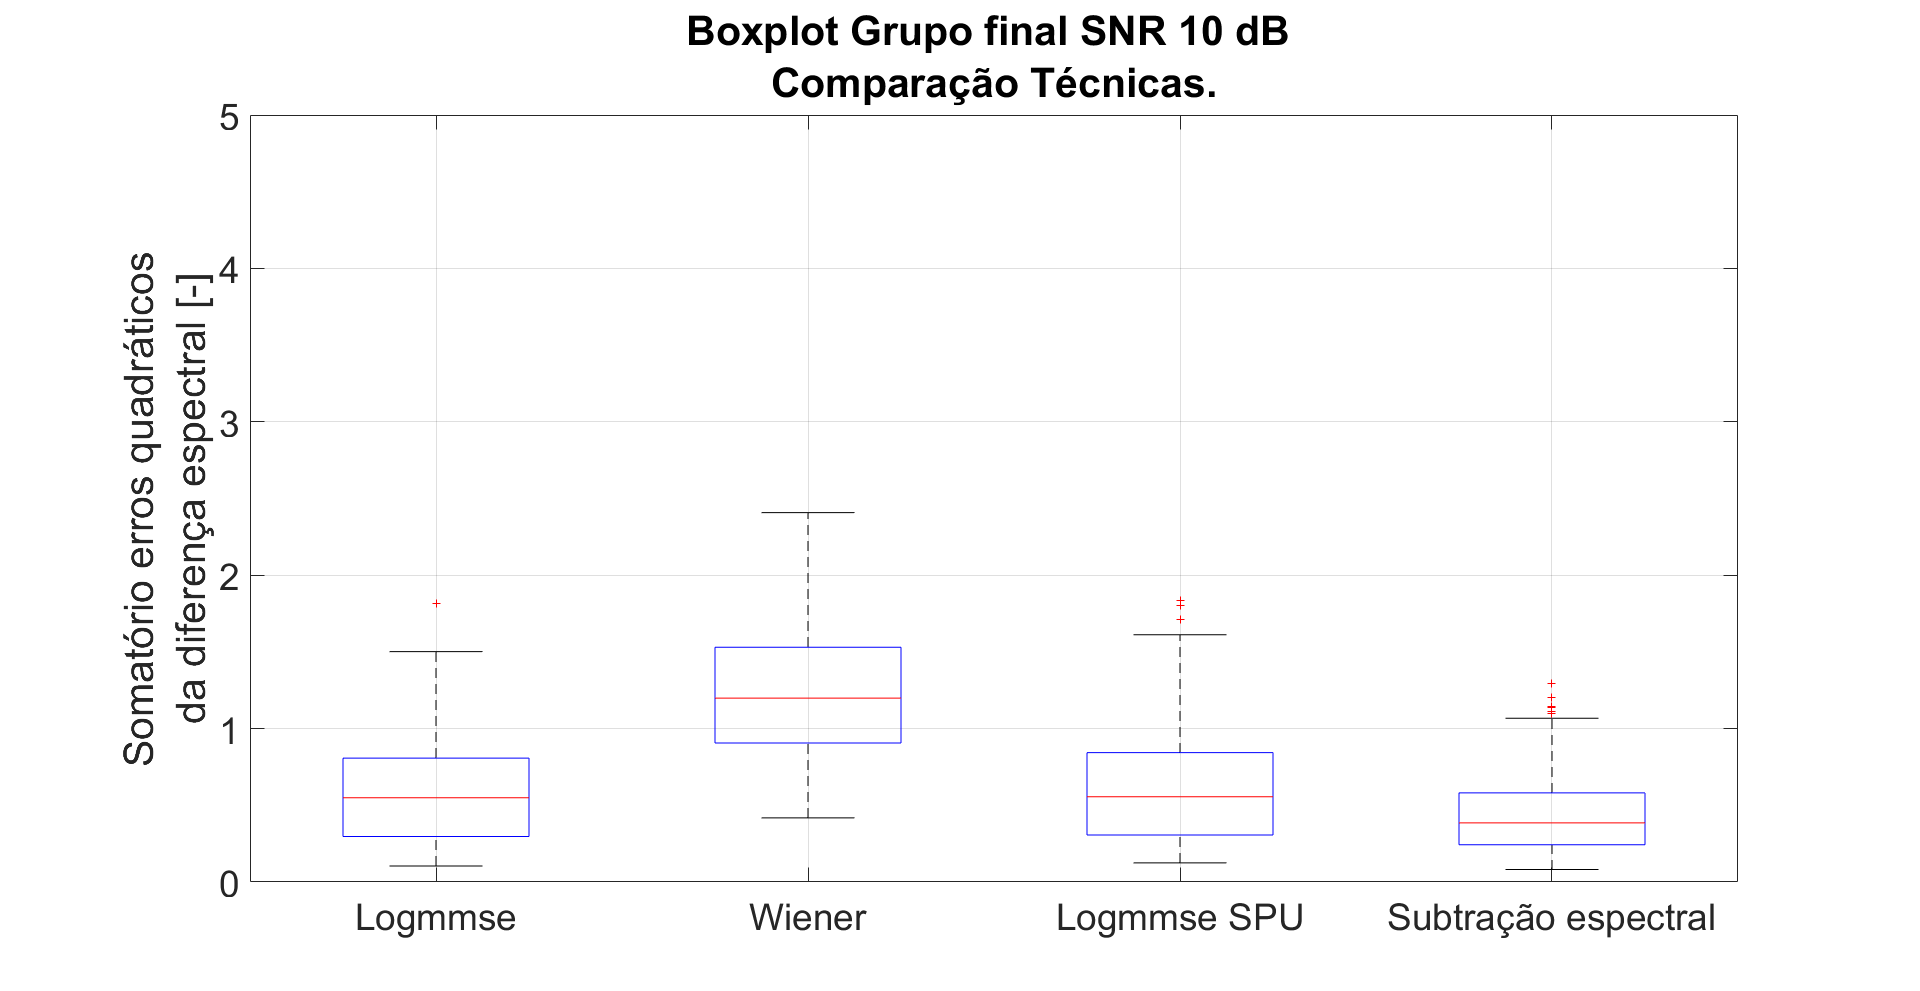
\includegraphics[width=8.5cm]{Figs/Total_10a}
\caption{Erro médio quadrático com SNR 10 dB para as técnicas utilizadas.}
\label{total_m10}
\end{figure}

A avaliação das medianas do erro quadrático médio para as diferentes técnicas é apresentada na \figura{total_total}

\begin{figure}[H]
\centering
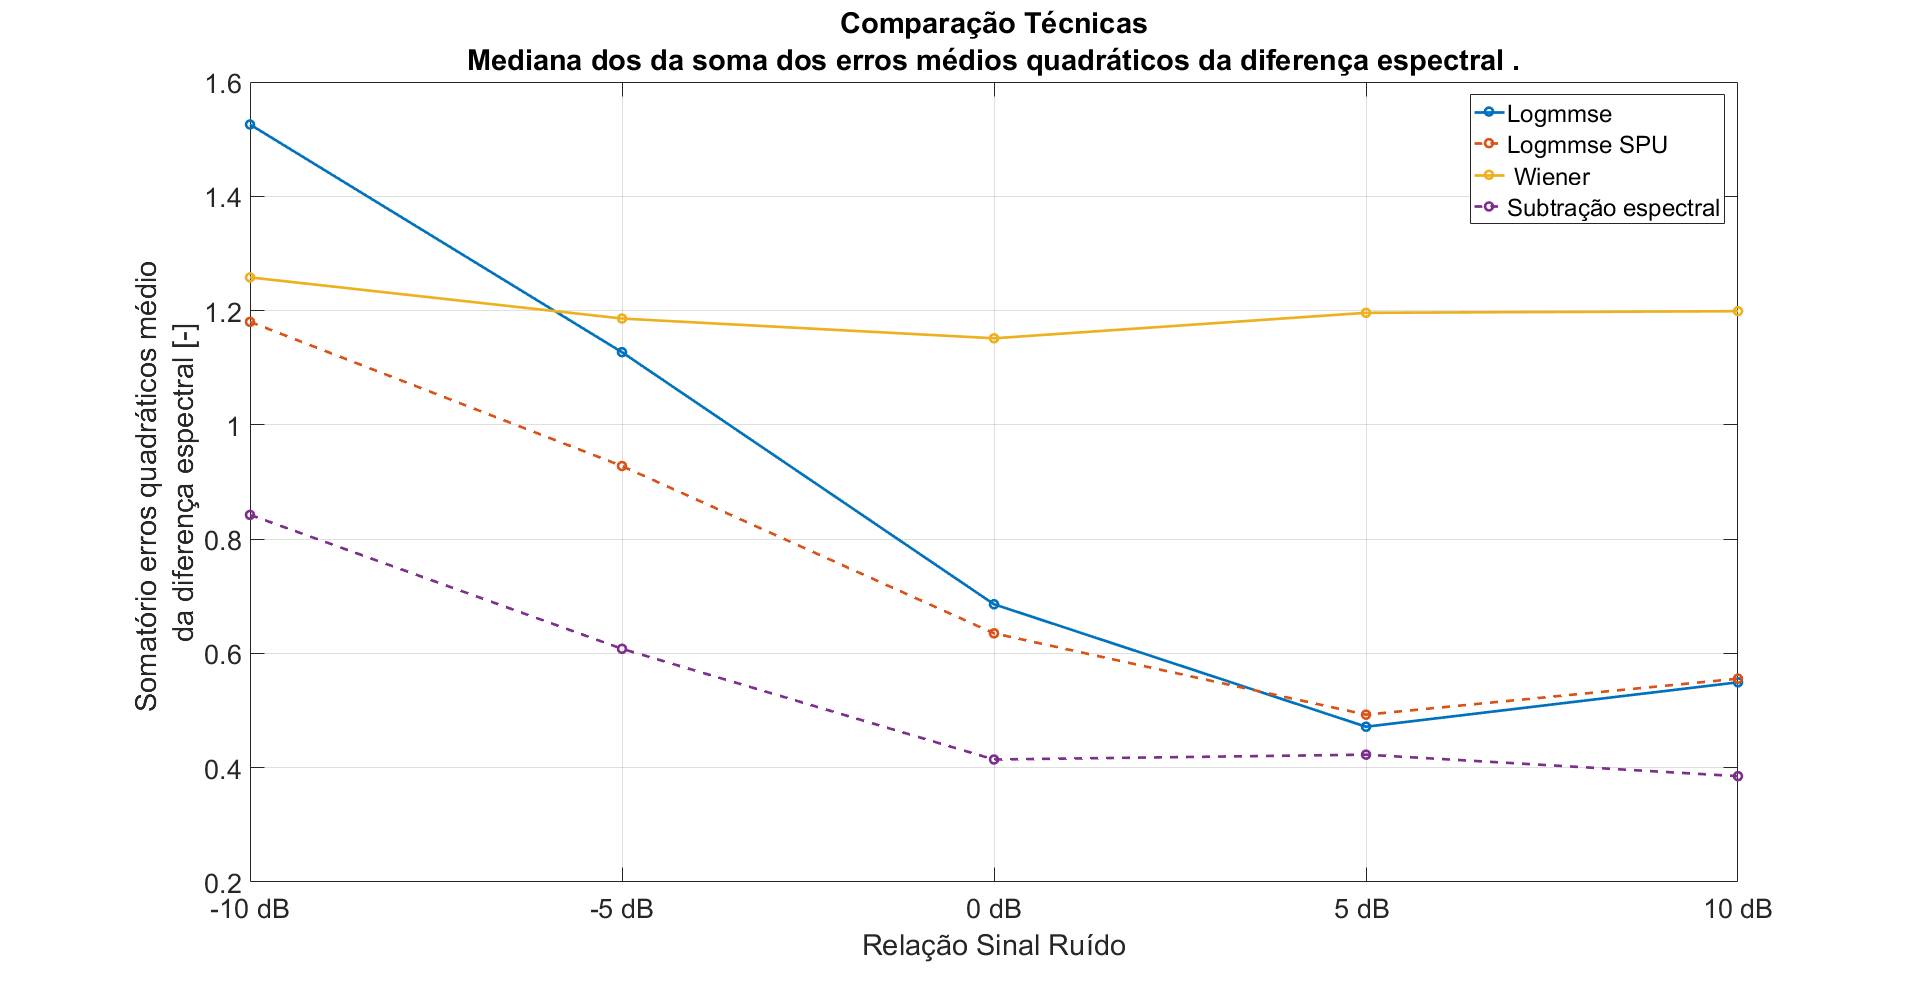
\includegraphics[width=14cm]{Figs/Total_total}
\caption{Erro médio quadrático por SNR para as técnicas utilizadas.}
\label{total_total}
\end{figure}



\section{Avaliação subjetiva}
A avaliação subjetiva (pré teste) proposta no trabalho foi realizada entre o sinal não processado e o sinal contaminado e processado com a técnica de filtragem Wiener iterativo. Os áudios foram carregados em uma interface do Matlab que permite a alternância entre dois sinais.

A pergunta realizada aos sujeitos do pré-teste subjetivo foi: ``Comparando os dois sinais, qual a nota para cada um quanto a inteligibilidade da fala?"
    
\begin{itemize}
        \item 27 comparações (pares)
        \item tempo médio 20 minutos
\end{itemize}

O pré teste foi realizado com 2 alunos, um de pós graduação e um de graduação não envolvidos e sem treinamento na questão de processamento da fala na tarde de 13 de outubro em uma sala sem tratamento acústico com fones Sennheiser HD 650 em volume controlado pelo ouvinte em ordem crescente de SNR.

As notas foram graduadas de 0 a 5 em números inteiros para cada sinal, onde 0 é ininteligível e 5 confortavelmente inteligível. Os resultados estão dispostos na \tabela{tabelasub}.

\begin{table}[H]
\centering
\caption{Resultados da avaliação subjetiva}
\label{tabelasub}
\resizebox{\textwidth}{!}{%
\begin{tabular}{cccccccccc}
 & \multicolumn{9}{c}{Nota média 2 avaliadores} \\
\multirow{-2}{*}{} & \cellcolor[HTML]{FFFFFF}\begin{tabular}[c]{@{}c@{}}Ruido 1 \\ SNR -10\end{tabular} & \begin{tabular}[c]{@{}c@{}}Ruido 2 \\ SNR -10\end{tabular} & \begin{tabular}[c]{@{}c@{}}Ruido 3 \\ SNR -10\end{tabular} & \cellcolor[HTML]{FFFFFF}\begin{tabular}[c]{@{}c@{}}Ruido 1 \\ SNR 0\end{tabular} & \begin{tabular}[c]{@{}c@{}}Ruido 2 \\ SNR 0\end{tabular} & \begin{tabular}[c]{@{}c@{}}Ruido 3 \\ SNR 0\end{tabular} & \begin{tabular}[c]{@{}c@{}}Ruido 1\\ SNR 10\end{tabular} & \begin{tabular}[c]{@{}c@{}}Ruido 2\\ SNR 10\end{tabular} & \multicolumn{1}{l}{\begin{tabular}[c]{@{}l@{}}Ruido 3\\ SNR 10\end{tabular}} \\
\rowcolor[HTML]{FFCCC9} 
Sinal 1 Contaminado & 1 & 1 & 2 & 3 & 2.5 & 2 & 4.5 & 4 & 4.5 \\
\rowcolor[HTML]{FFCCC9} 
Sinal 1 Wiener & 0 & 0 & 0 & 2 & 2 & 0 & 4 & 4 & 4 \\
\rowcolor[HTML]{FFFFC7} 
Sinal 2 Contaminado & 0 & 0 & 3 & 2 & 0 & 3 & 4 & 4 & 4 \\
\rowcolor[HTML]{FFFFC7} 
Sinal 2 Wiener & 0 & 0 & 0 & 2 & 2 & 0 & 3 & 3 & 4 \\
\rowcolor[HTML]{FFCCC9} 
Sinal 3 Contaminado & 0 & 1 & 2 & 0 & 2 & 3 & 3 & 4 & 4 \\
\rowcolor[HTML]{FFCCC9} 
Sinal 3 Wiener & 0 & 0 & 0 & 3 & 1 & 0 & 3 & 3 & 4
\end{tabular}%
}
\end{table}

Observações anotadas: para vários ruídos a supressão de Wiener cortou a informação do sinal, e a nota com a fala sem filtragem foi melhor, visto que não havia fala para avaliar no áudio filtrado. Como exemplo os espectrogramas das \figuras{aff3} a \fign{aff5}, referentes ao sinal 3 contaminados pelo ruído 3, apresentam esse efeito.

\begin{figure}[H]
\subfloat[Sinal de fala.]{\label{tm102}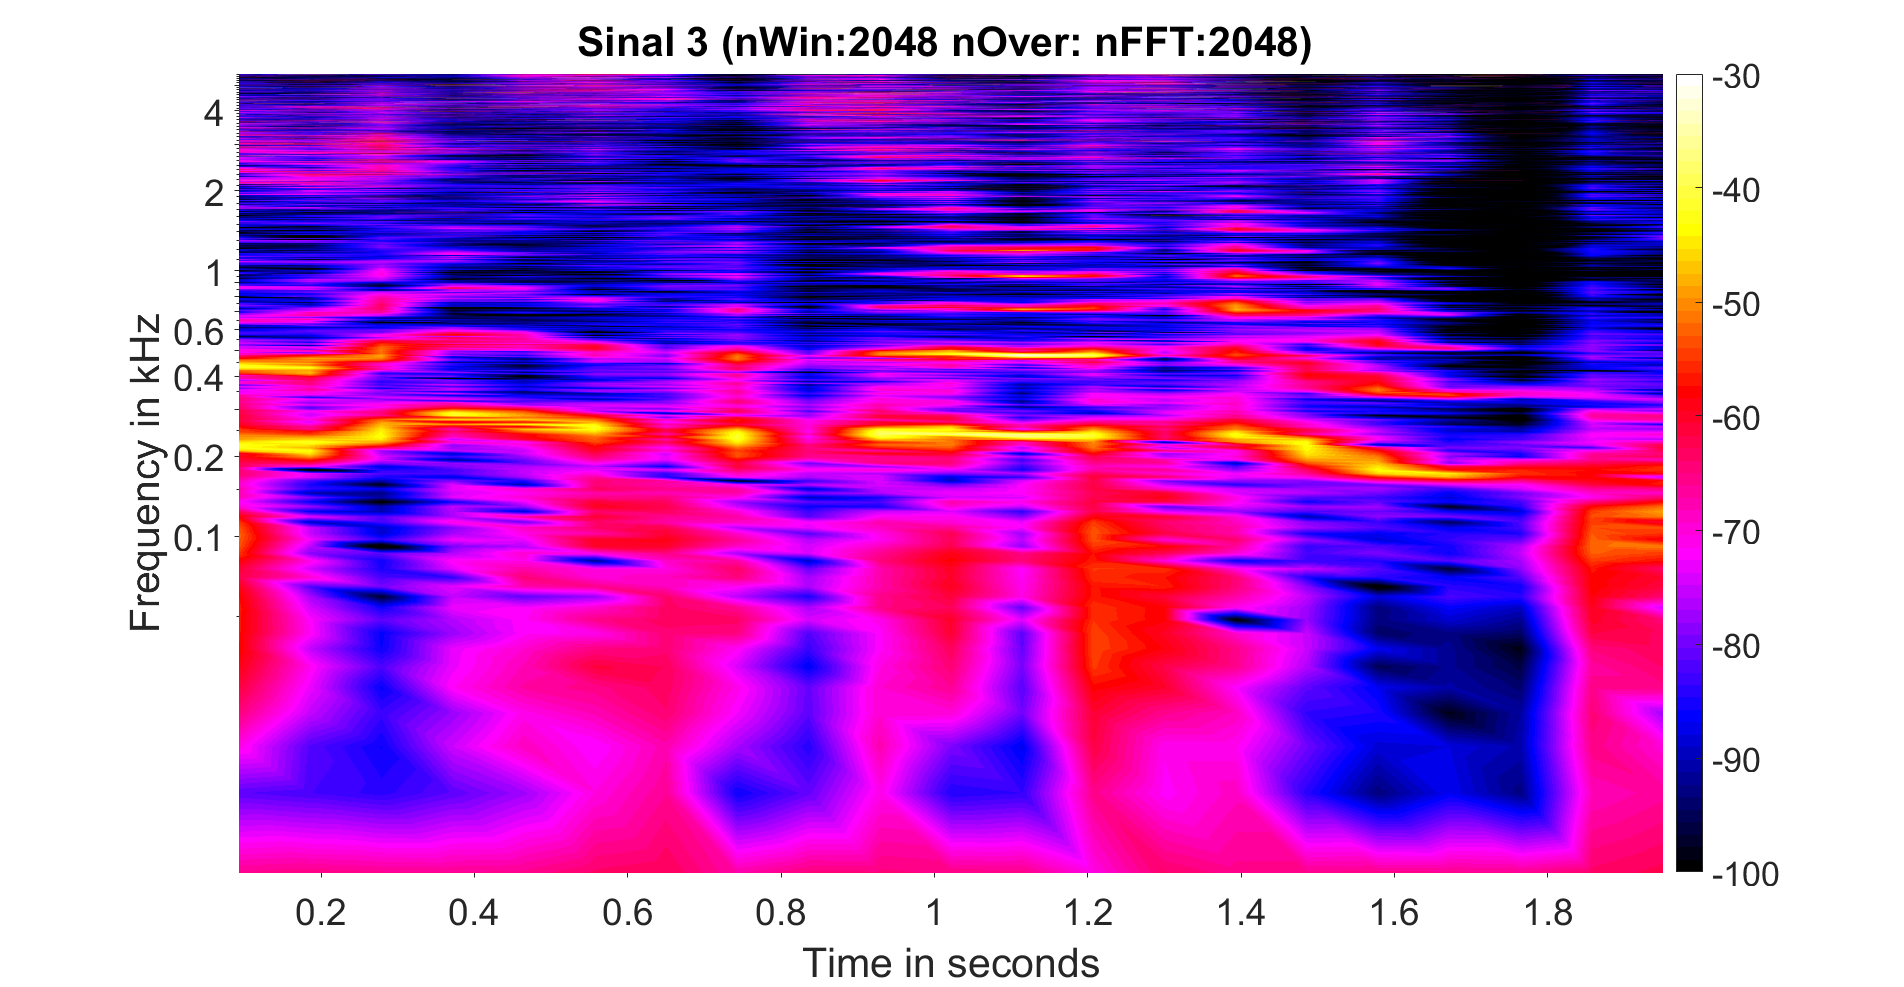
\includegraphics[width=8.5cm,]{Figs/s3}}\quad
\subfloat[Ruído contaminante.]{\label{tm52}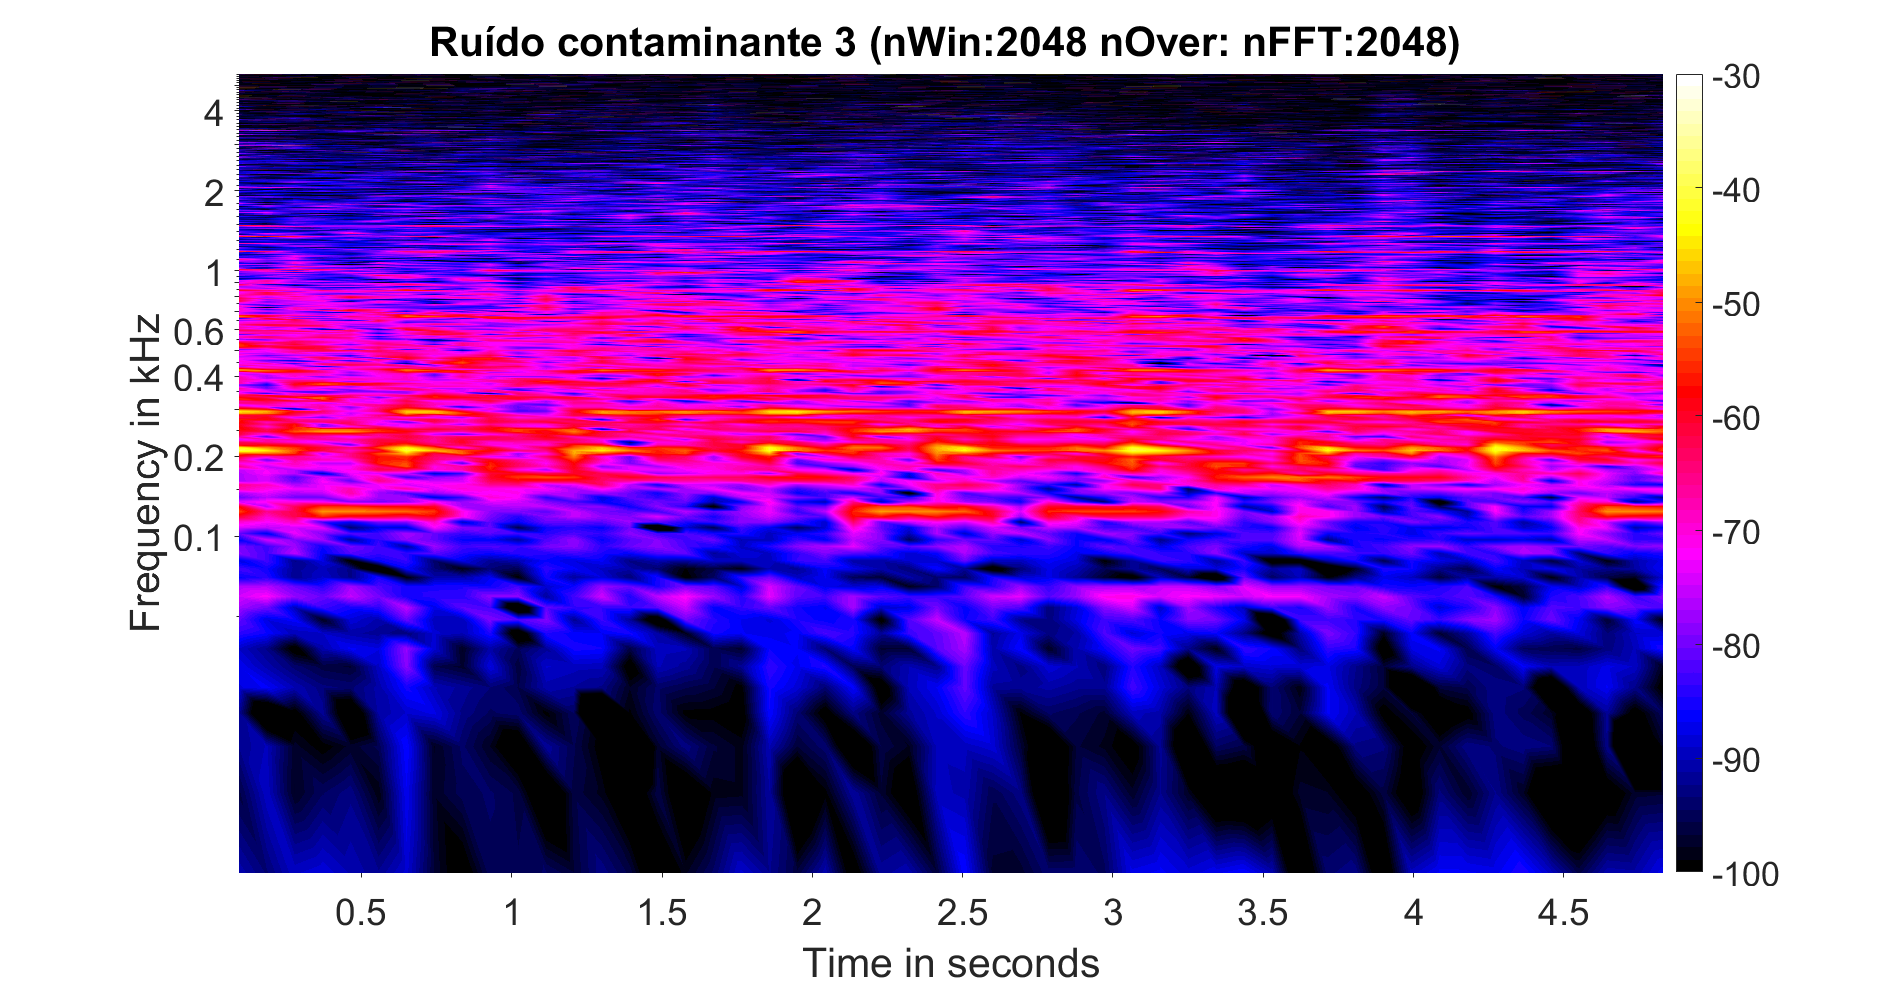
\includegraphics[width=8.5cm,]{Figs/ruido3}}
\caption{Espectros do sinal de fala e do ruído contaminante.}
\label{aff3}
\end{figure}

\begin{figure}[H]
\subfloat[SNR -10 dB.]{\label{snr-10np}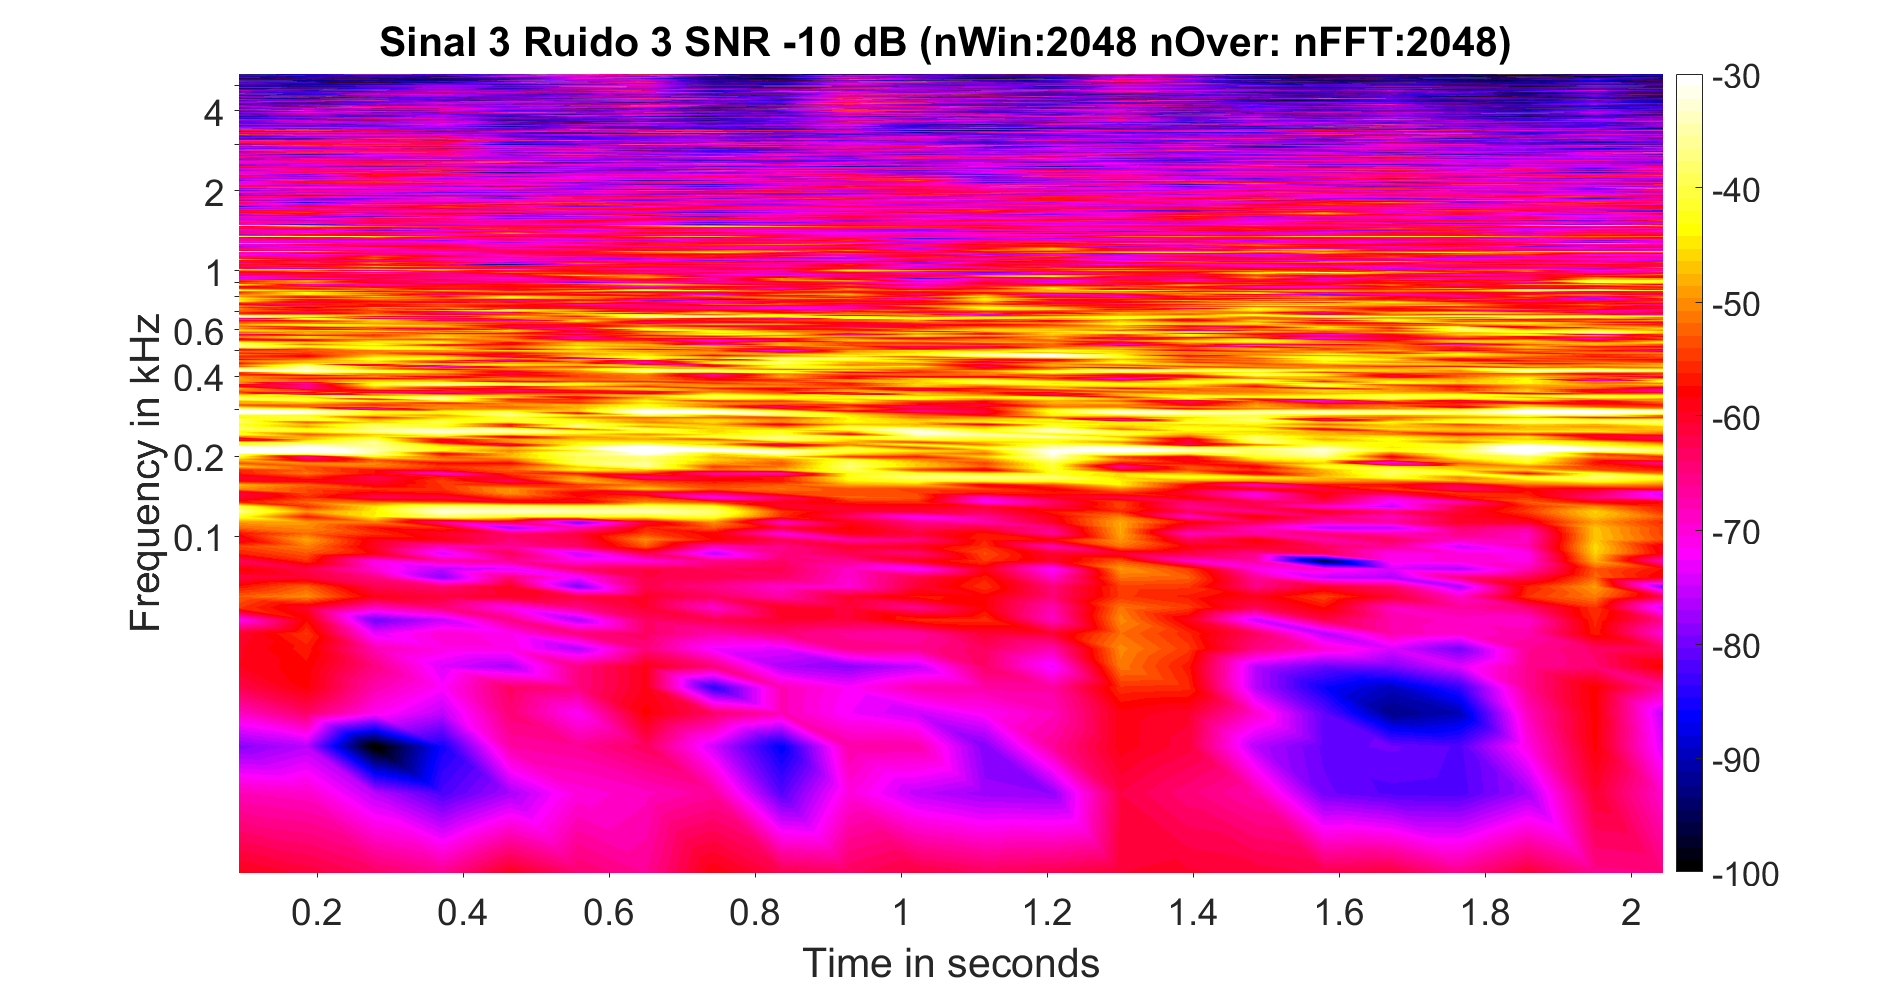
\includegraphics[width=8.5cm,]{Figs/ruido3s3contaminado.png}}\quad
\subfloat[SNR -10 dB.]{\label{snr-10w}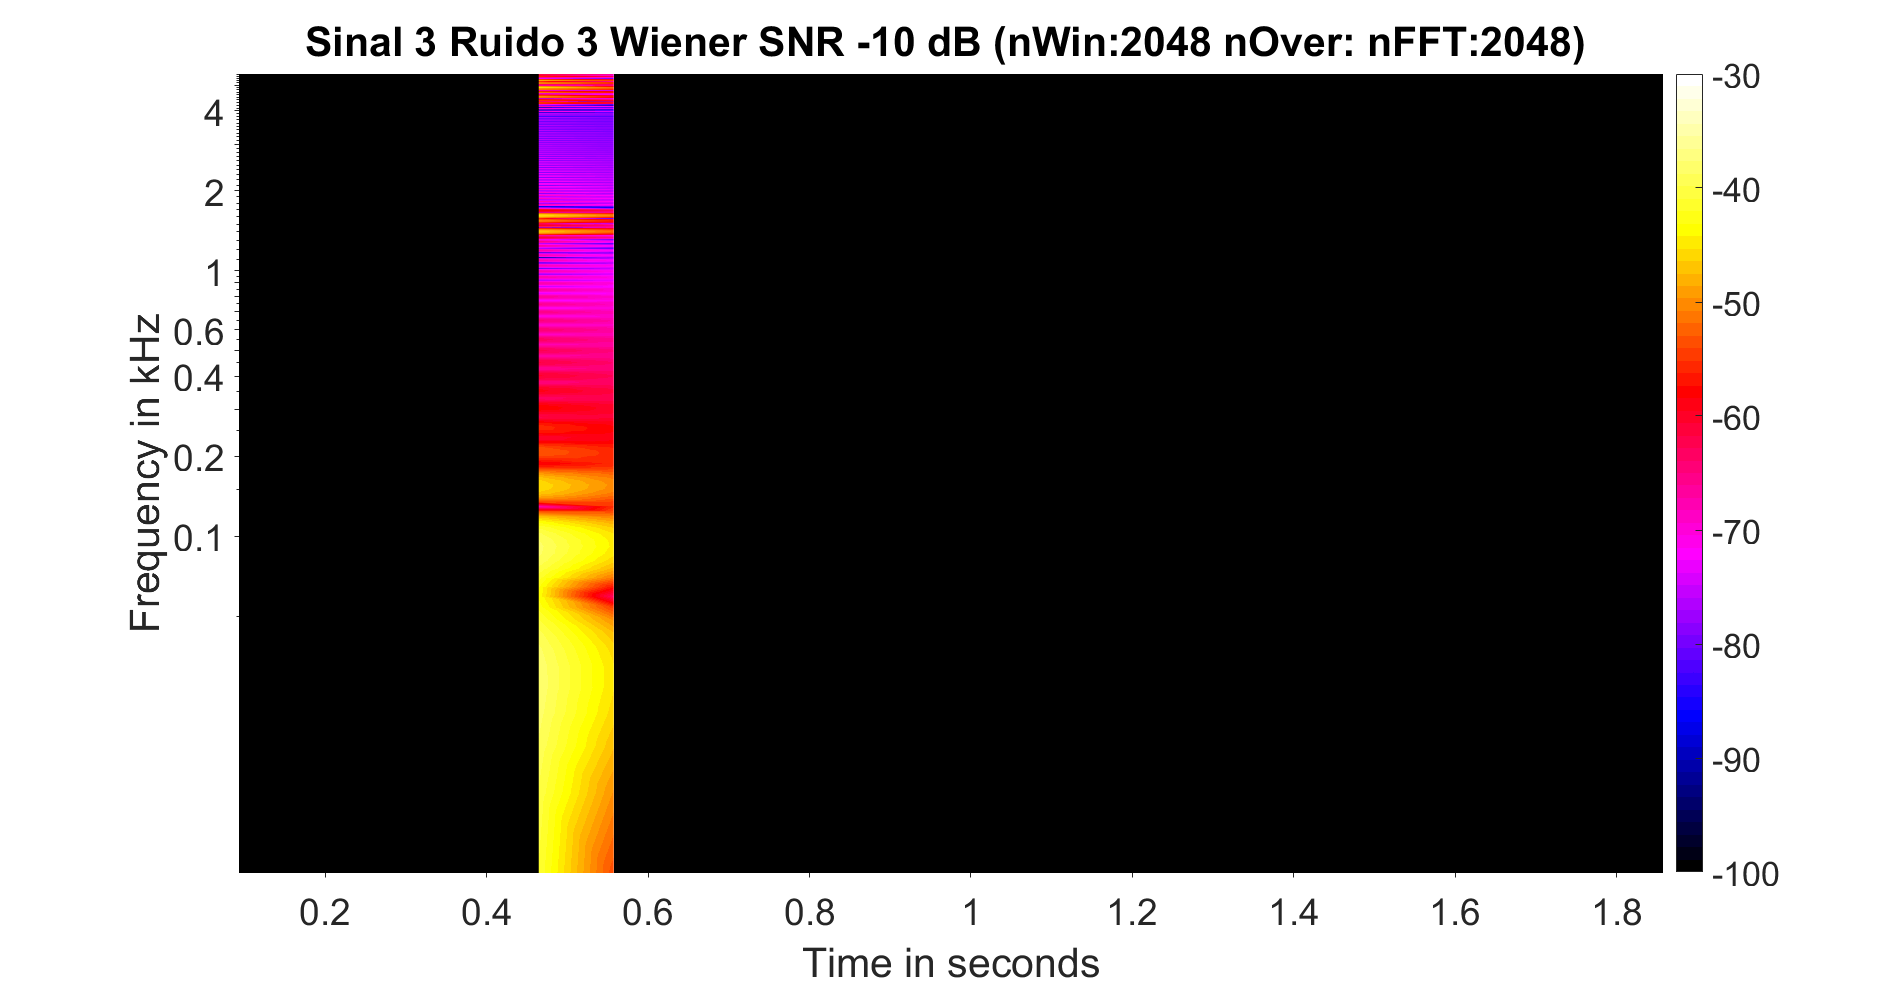
\includegraphics[width=8.5cm,]{Figs/ruido3s3_wiener}}
\caption{Espectros do sinal sem processamento e com a filtragem de Wiener.}
\label{aff4}
\end{figure}

\begin{figure}[H]
\subfloat[SNR 0 dB.]{\label{snr-10np}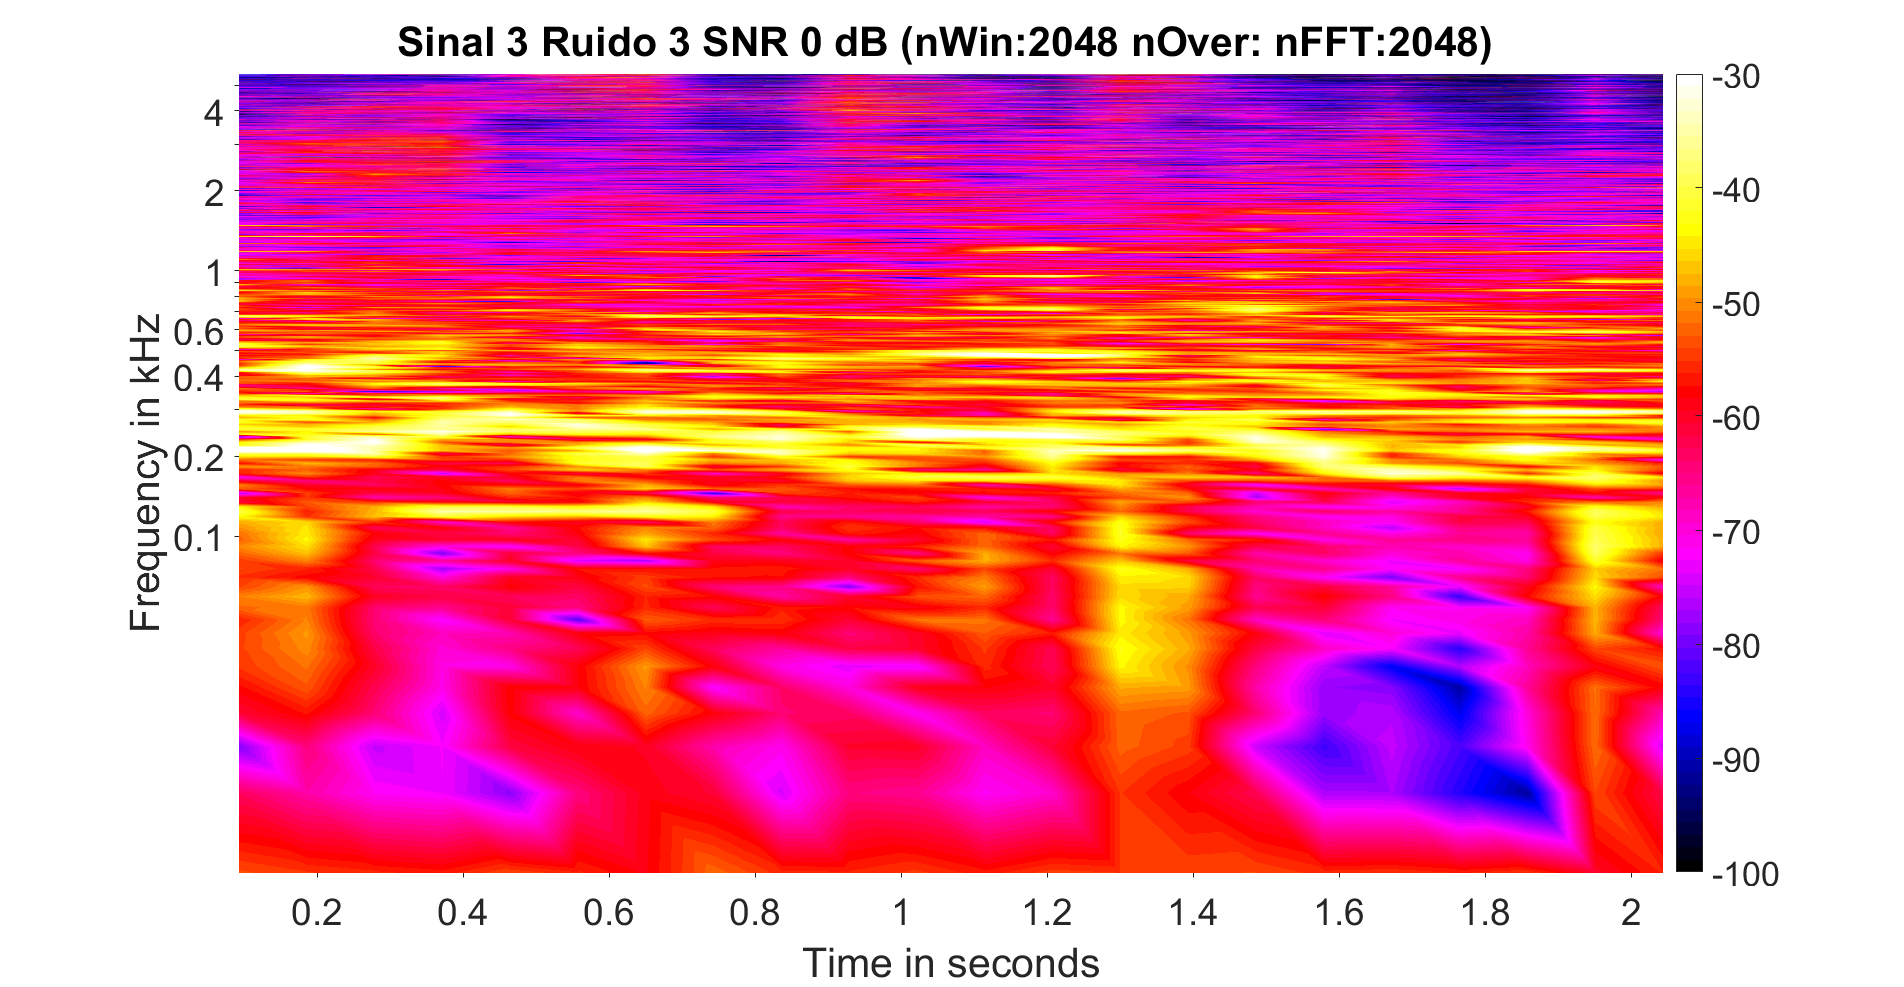
\includegraphics[width=8.5cm,]{Figs/ruido3s3contaminado0db.png}}\quad
\subfloat[SNR 0 dB.]{\label{snr-10w}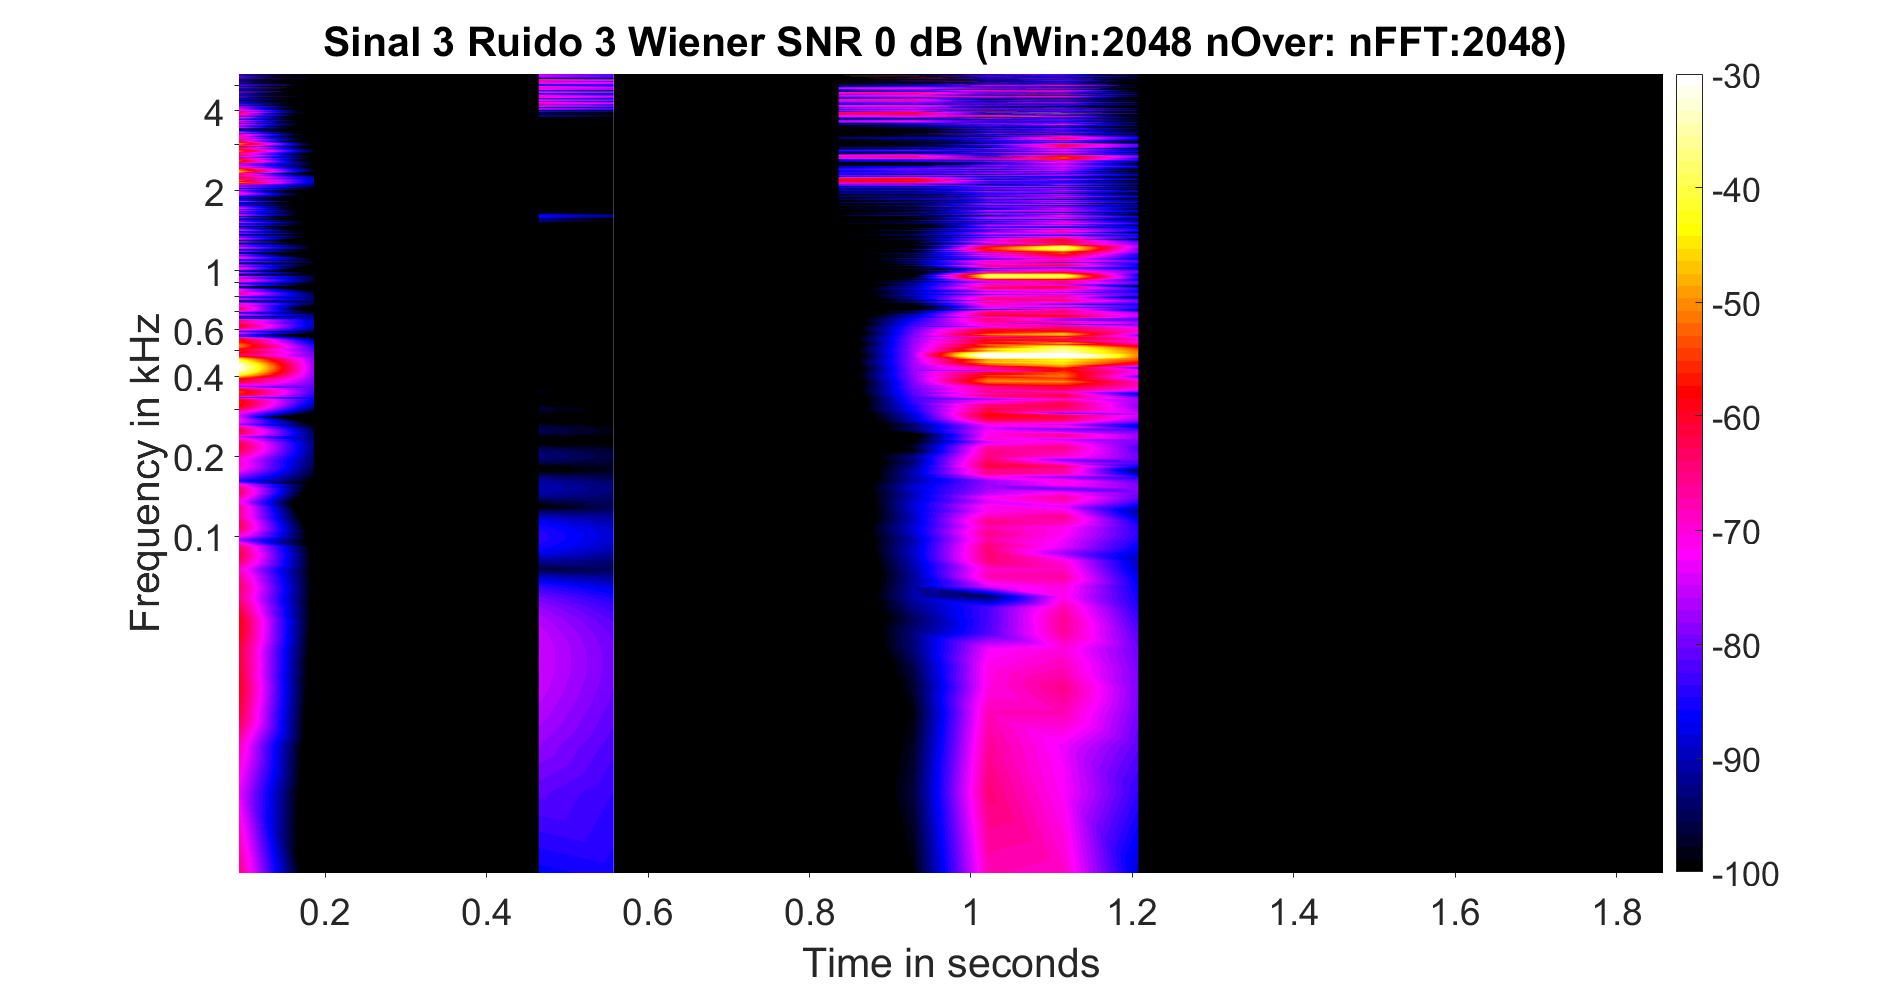
\includegraphics[width=8.5cm,]{Figs/ruido3s3_wiener0db}}
\caption{Espectros do sinal sem processamento e com a filtragem de Wiener.}
\label{aff5}
\end{figure}


\begin{figure}[H]
\subfloat[SNR 10 dB.]{\label{snr-10np}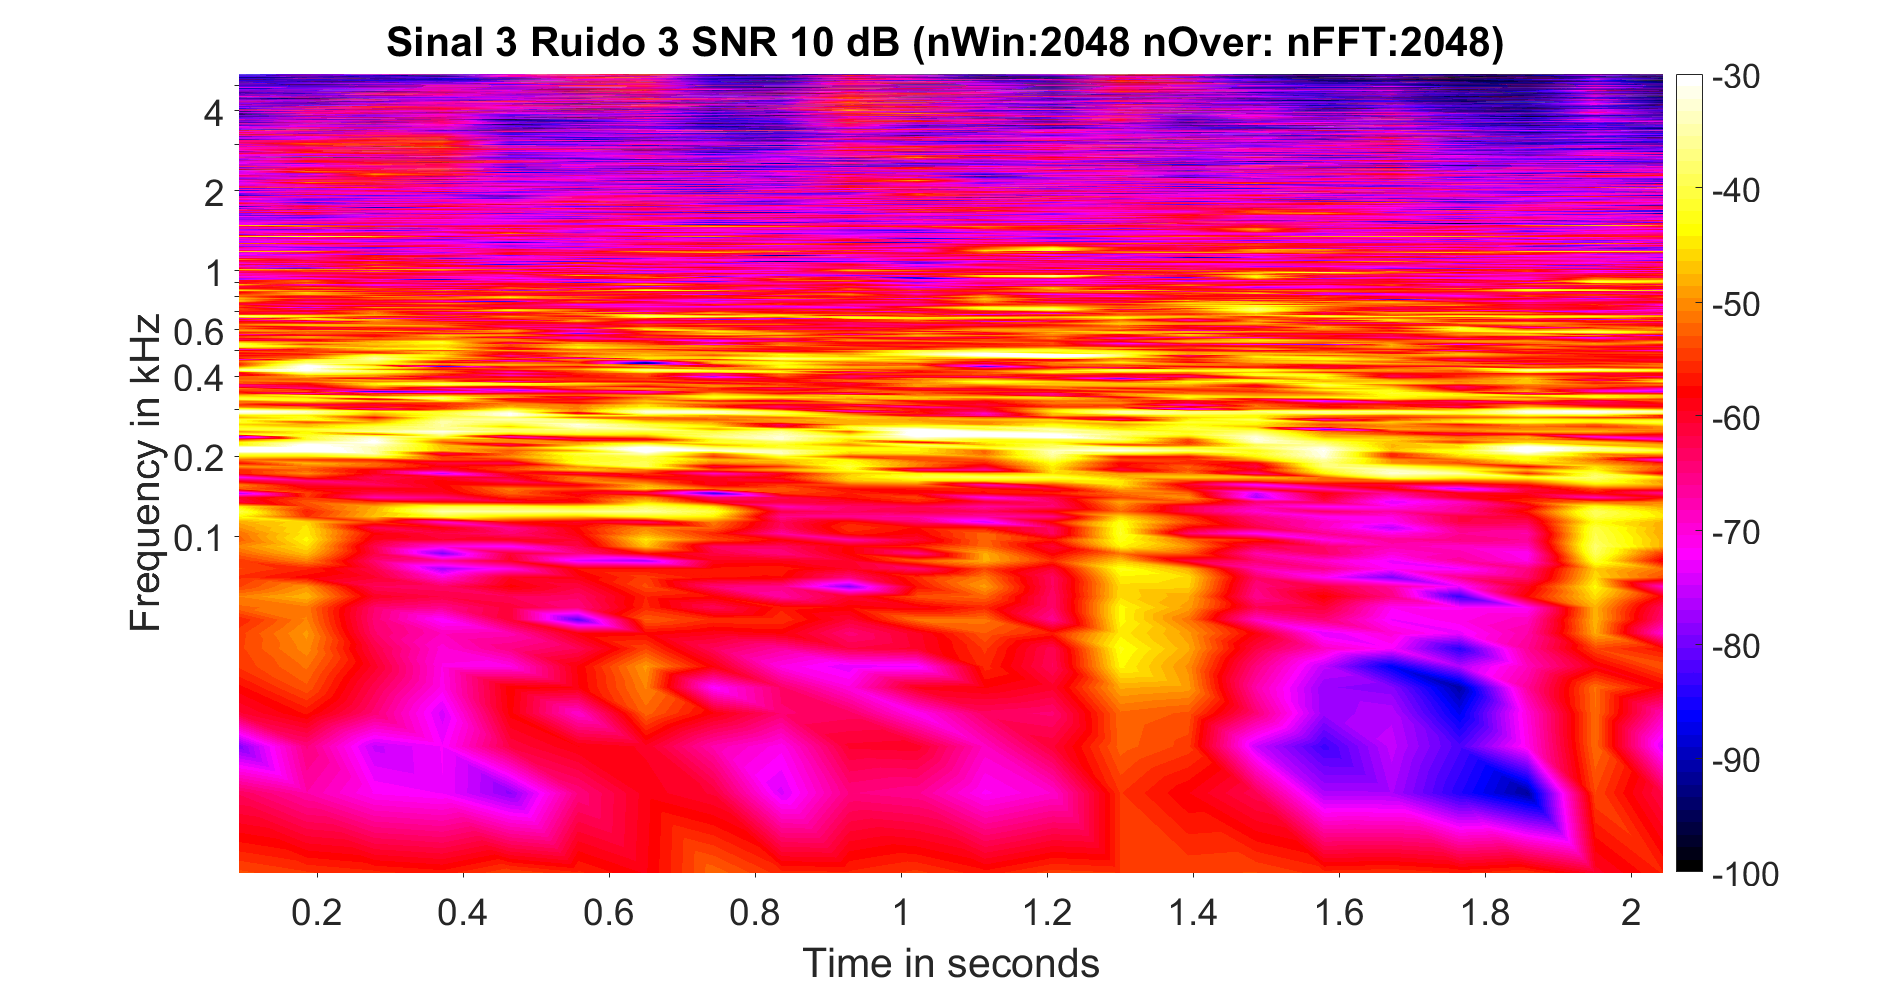
\includegraphics[width=8.5cm,]{Figs/ruido3s3contaminado10db.png}}\quad
\subfloat[SNR 10 dB.]{\label{snr-10w}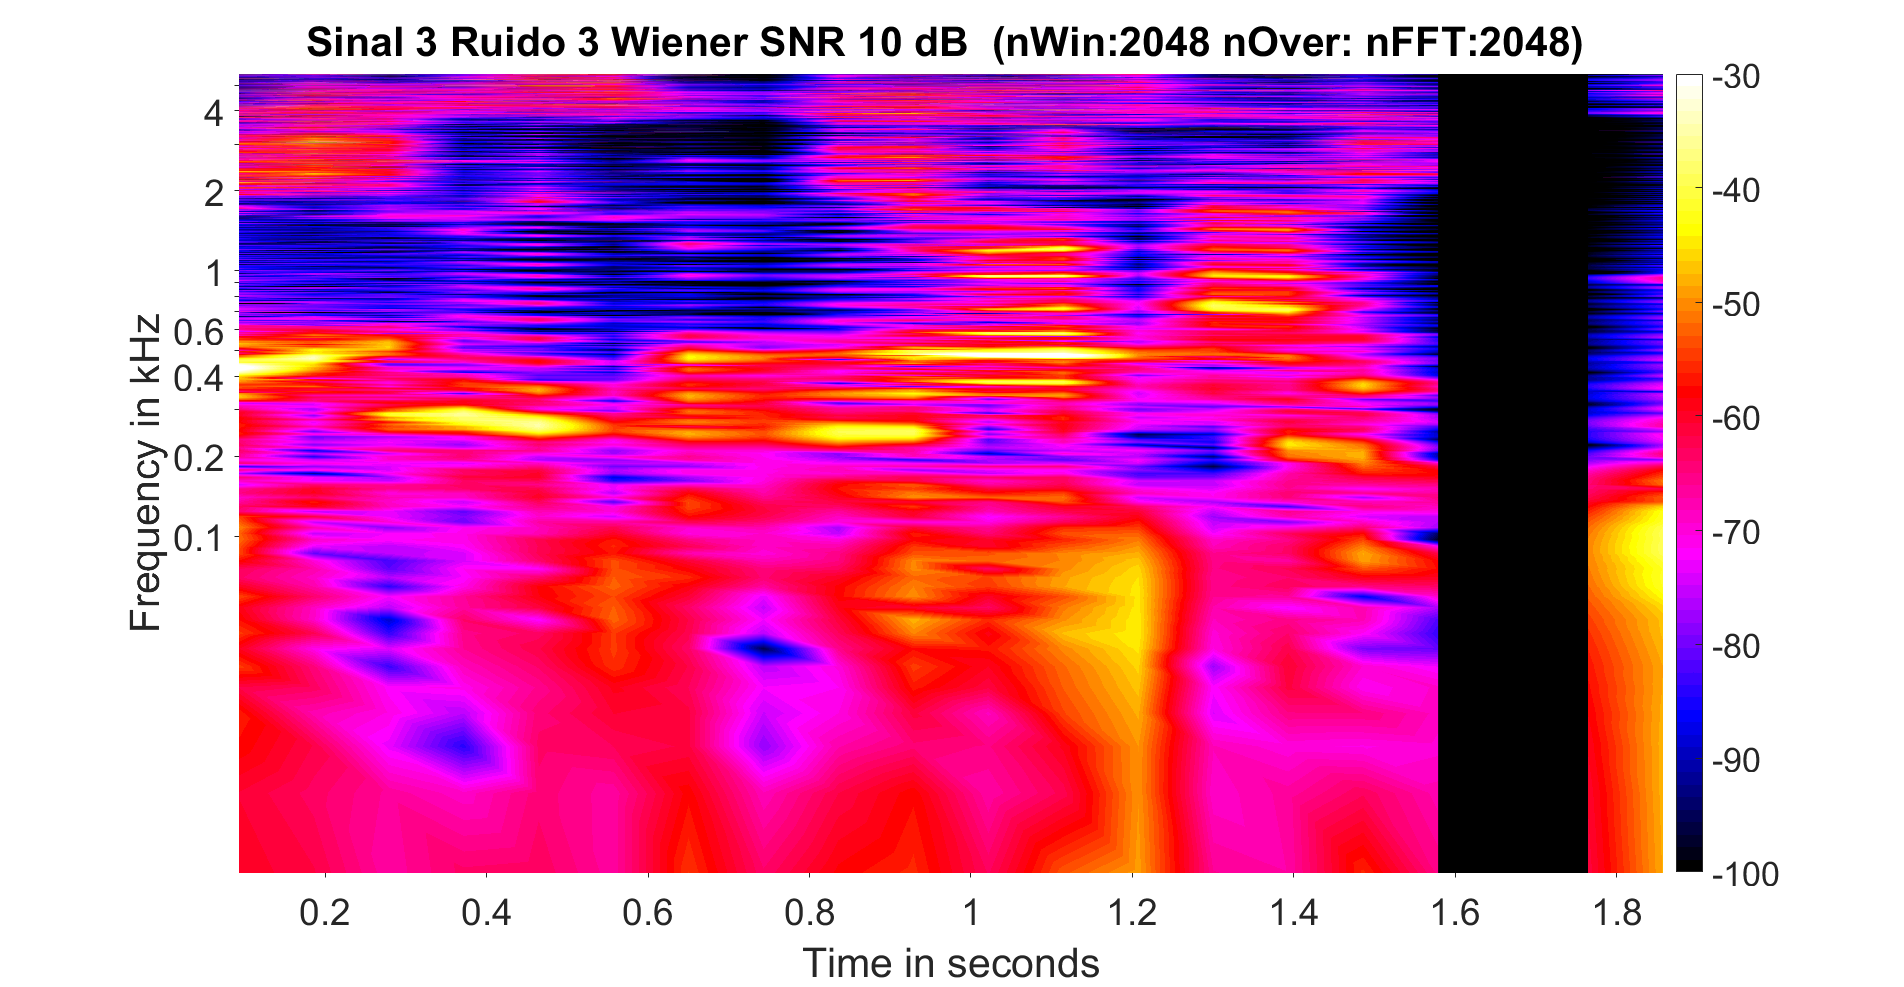
\includegraphics[width=8.5cm,]{Figs/ruido3s3_wiener10db}}
\caption{Espectros do sinal sem processamento e com a filtragem de Wiener.}
\label{aff5}
\end{figure}


Houve uma tendência de crescimento da inteligibilidade com maior SNR, contudo há a preferência do sinal contaminado, o sinal processado a técnica de filtragem de Wiener não obteve boas avaliações.

A filtragem de Wiener, através da mediana dos erros médios quadráticos tem uma melhor performance em frente ao sinal não processado, ver \figura{versus}, o que não conjurou com o resultado subjetivo. 

\begin{figure}[H]
\centering
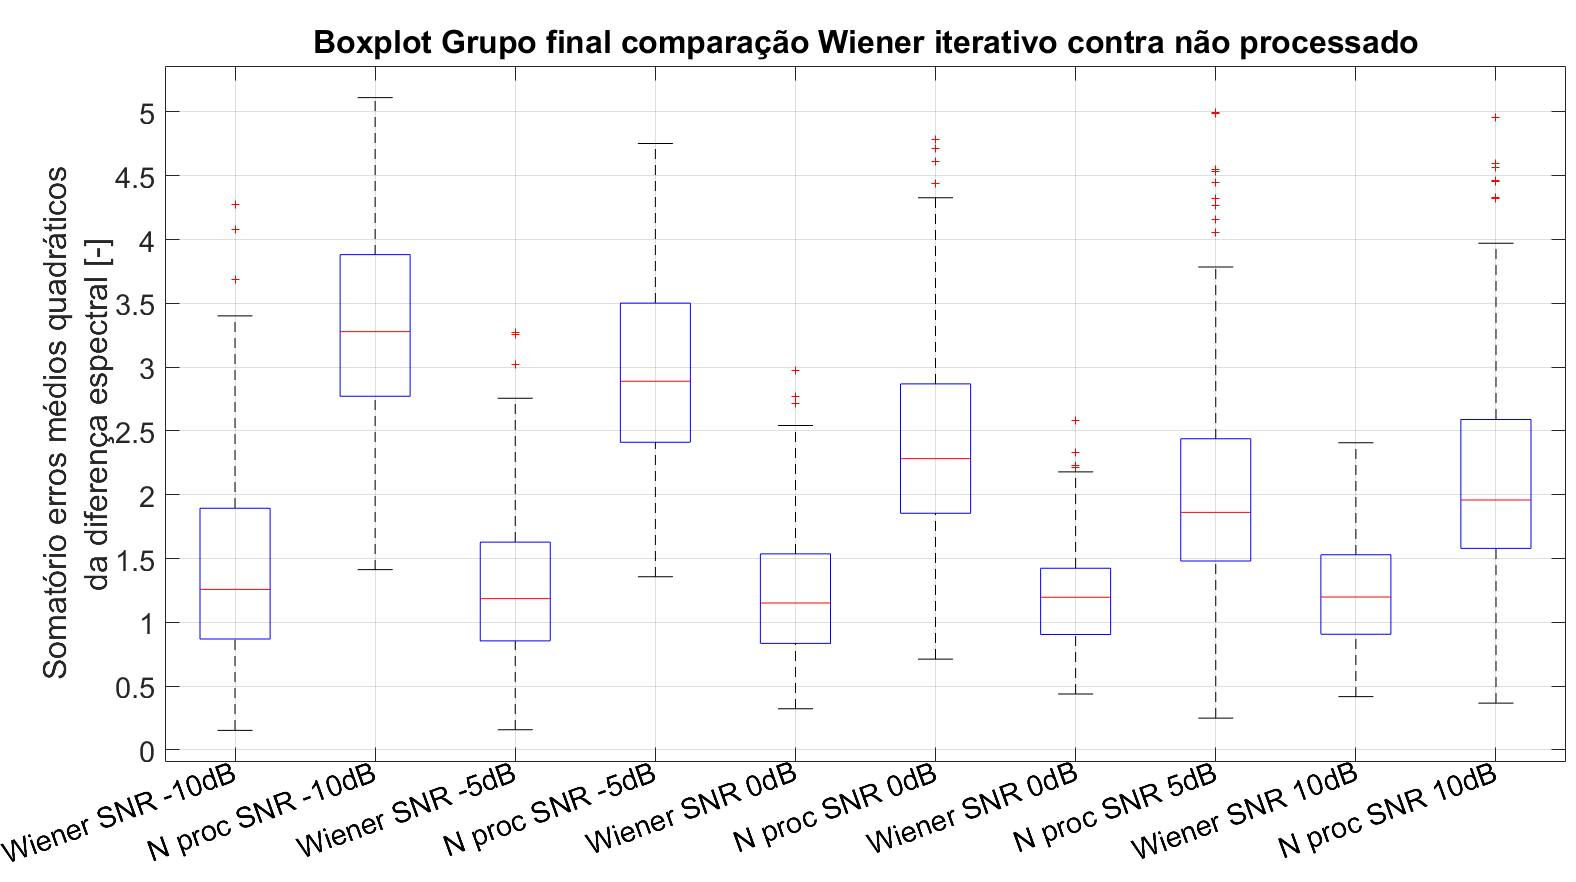
\includegraphics[width=14cm]{Figs/comparacao_wiener_Nproc}
\caption{Erro médio quadrático por SNR Wiener e sinal não processado.}
\label{versus}
\end{figure}


\chapter{Conclusões}
Existem parâmetros que auxiliam na diminuição do erro médio quadrático, e eles podem ser dimensionados a partir de análises de grupos prévios como feito nesse trabalho. O resultado pode corroborar para a adequação da técnica escolhida ou até mesmo para a escolha de uma técnica.

Ainda que a escolha dos métodos tenha partido de um critério objetivo, no caso a mediana do erro médio quadrático entre a diferença espectral para a referência sendo o sinal de fala original, a tendência é de que a sensação subjetiva não corrobora com tal métrica. A avaliação dos algoritmos de processamento avaliados portando não tem uma classificação adequada partindo desse princípio.

O ajuste de parâmetros realizado com o grupo prévio pode otimizar as rotinas de processamento e ao final foram realizados testes subjetivos que contrapuseram a avaliação objetiva entre sinal não processado e sinal processado com a técnica de filtragem de Wiener iterativo. É provável que a não consideração de pesos na contabilização do erro quanto a localização da frequência (maior peso para frequências da fala) pode inferir em erro de mérito subjetivo. Uma proposta poderia ser avaliar com pesos de curvas de ponderação psicoacústica.


\chapter{Avaliação de desempenho}
Nesta seção serão apresentados as análises e avaliações dos métodos de redução de ruído, tanto objetivas quanto subjetivas
\section{Introdução}
A avaliação do desempenho dos algoritmos é um passo importante, dado que, dados subjetivos são custosos e laborais, ainda que a melhor ferramenta atualmente. Contudo é possível analisar certos problemas de melhoramento em degradação da fala a partir de modelos consagrados e bastante confiáveis, dentro de especificidades dos sinais propostos.

Avaliações objetivas tem o caráter de tentar quantificar a resposta à inteligibilidade ou qualidade da fala para que possa-se avaliar e adequar métricas e técnicas para diferentes casos e tipos de ruídos, sons ambientes e falas nas mais variadas línguas. Tendo uma métrica confiável de avaliação objetiva, que represente a resposta subjetiva de um conjunto de sujeitos, o processo torna-se apenas computacional, economizando tempo e reduzindo o custo. As métricas são classificadas em dois tipos gerais: Intrusivas (dependem do conhecimento do sinal original) e não intrusivas (não dependentes do sinal original).

\section{Análises Propostas}
A segunda parte deste trabalho apresenta três medidas objetivas de qualidade e duas medidas de inteligibilidade. Além disso um procedimento de análise subjetiva e a análise de confiabilidade intra- e inter-avaliador para qualidade.

\section{Avaliação objetiva}

\subsection{Análise dos ruídos}
Os ruídos apresentados na primeira parte do trabalho são apresentados a seguir com a mesma nomenclatura, sendo

\begin{itemize}
    \item RESTAURANT\_LARGE.flac (RL\textit{i})
    \item RESTAURANT\_medium.flac (RM\textit{i})
    \item RESTAURANT\_MEXICO.flac (RMX\textit{i})
\end{itemize}

Onde $i=1 \ldots 5$ que denota os 5 trechos de ruído selecionados para cada um.

O espectrograma do ruído RL1 e RL2  é apresentado na \figura{SRL}, sendo os ruídos RL3, RL4 e RL5 omitidos do texto pela similaridade para maior fluência do texto.


\begin{figure}[H]
\subfloat[RL1]{\label{fRL1}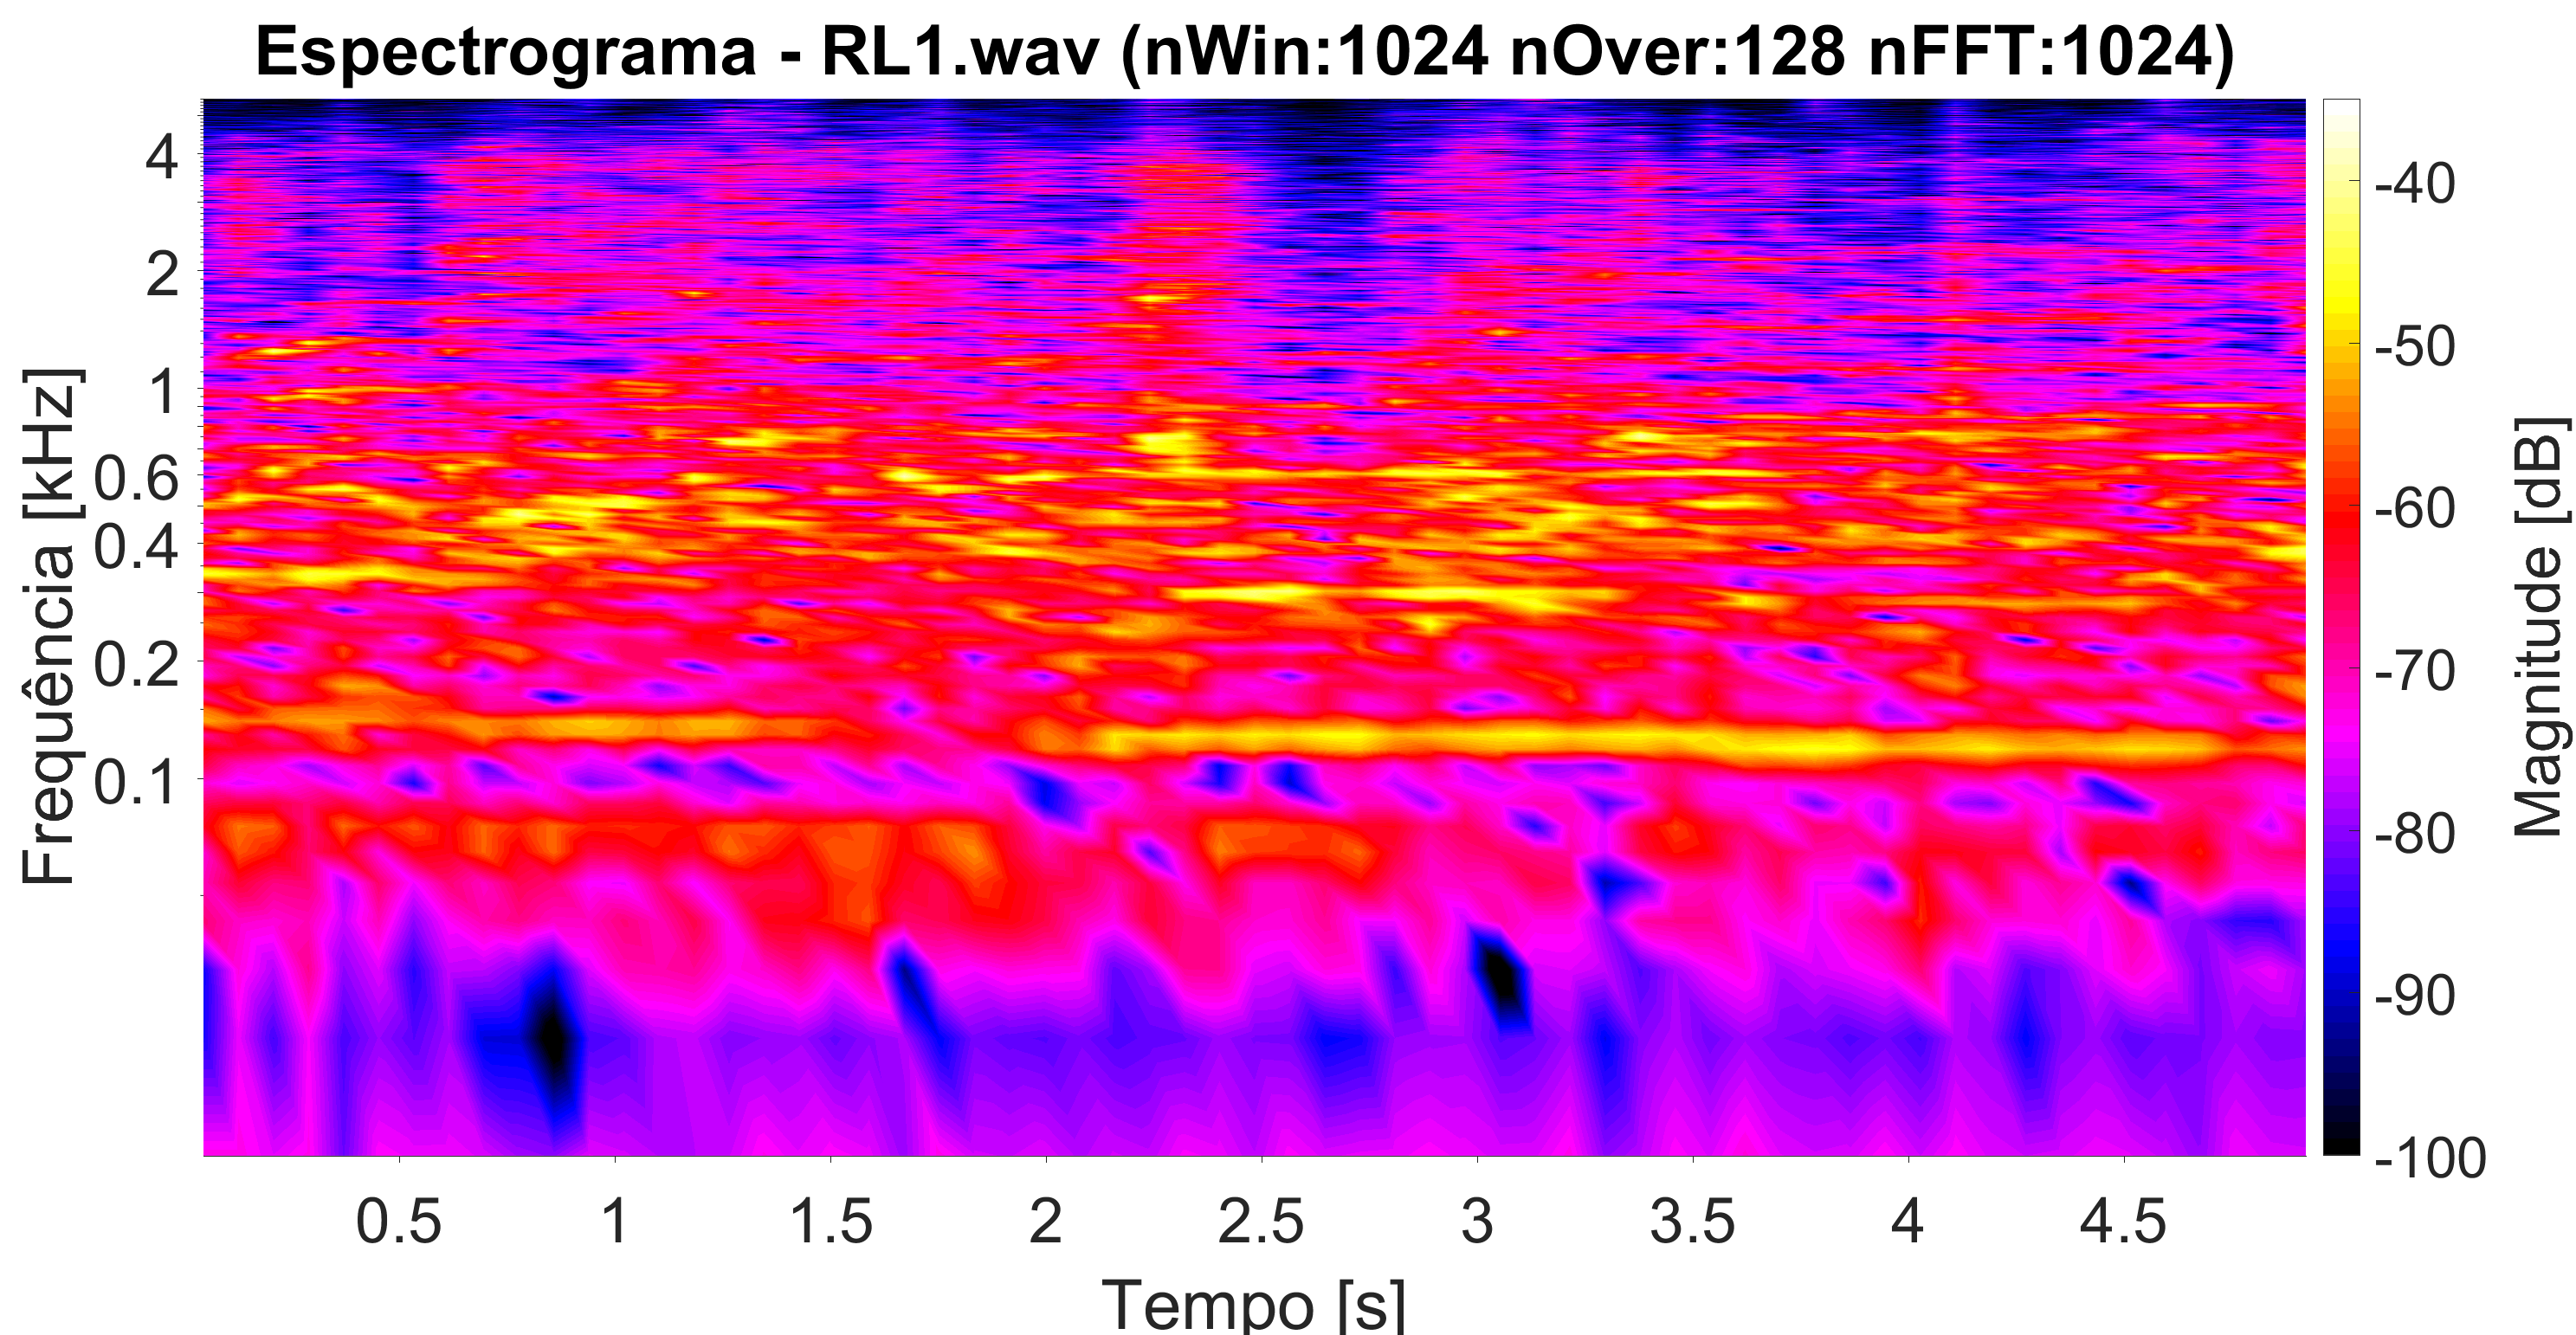
\includegraphics[width=8.5cm,]{Figs/RL1}}\quad
 \subfloat[RL2]{\label{fRL2}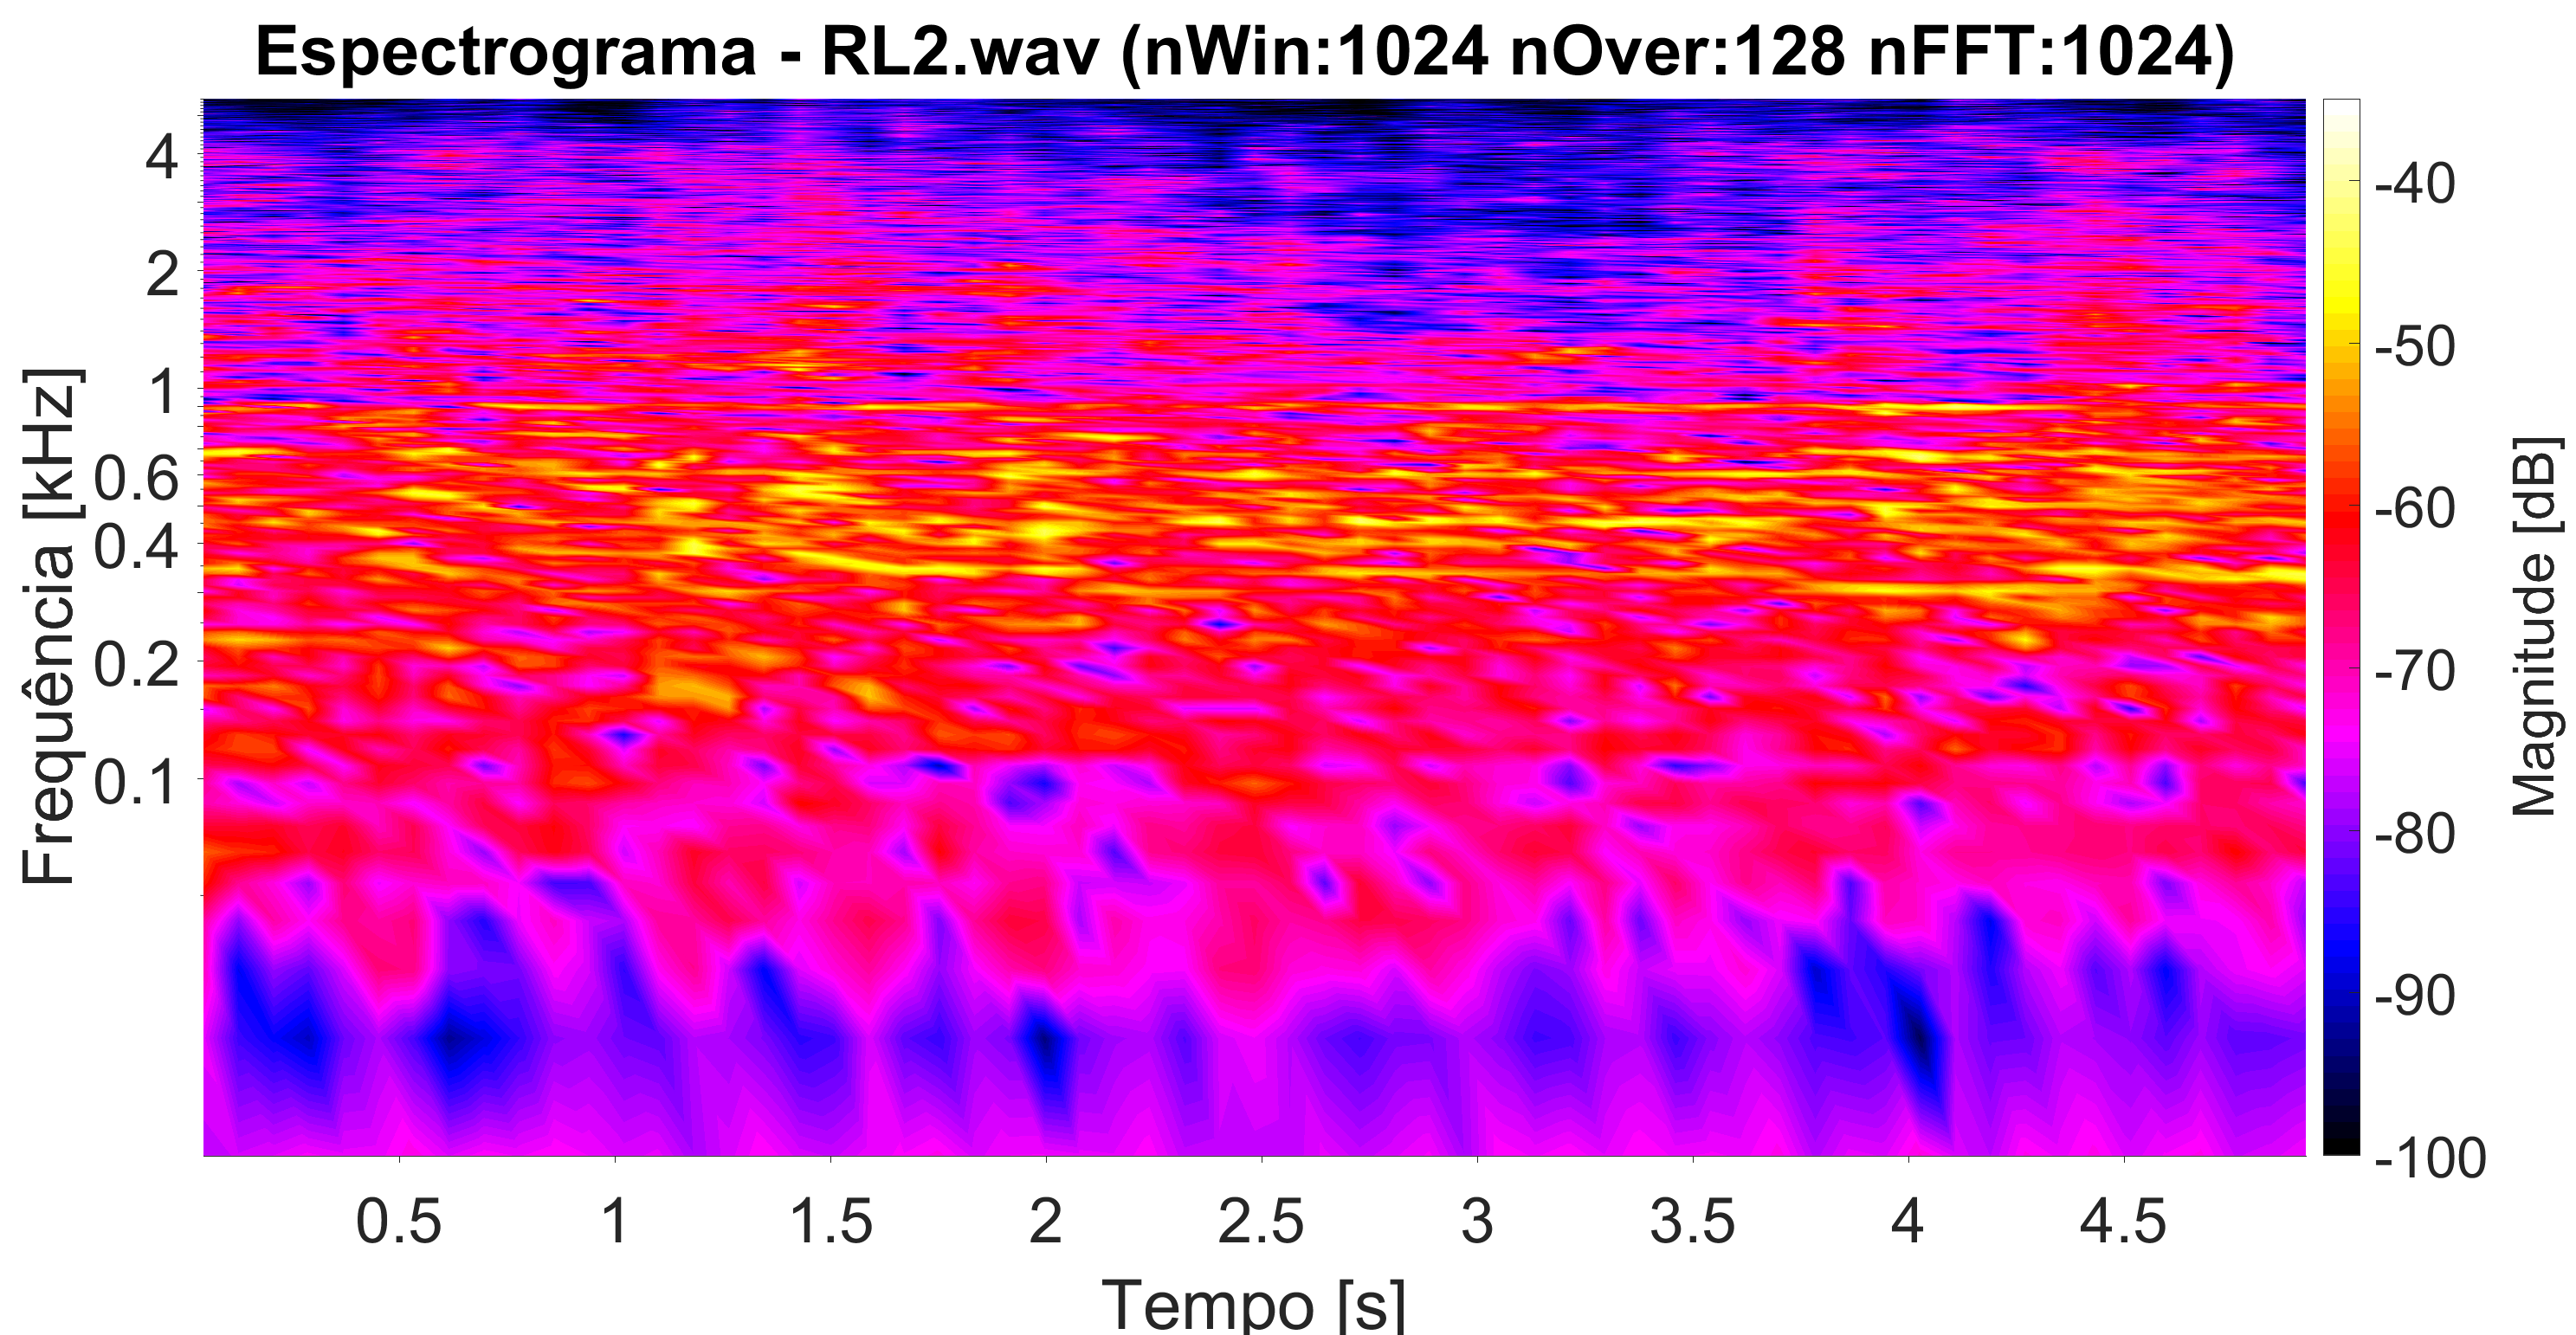
\includegraphics[width=8.5cm,]{Figs/RL2}} 
%\subfloat[asdasd]{\label{fRL3}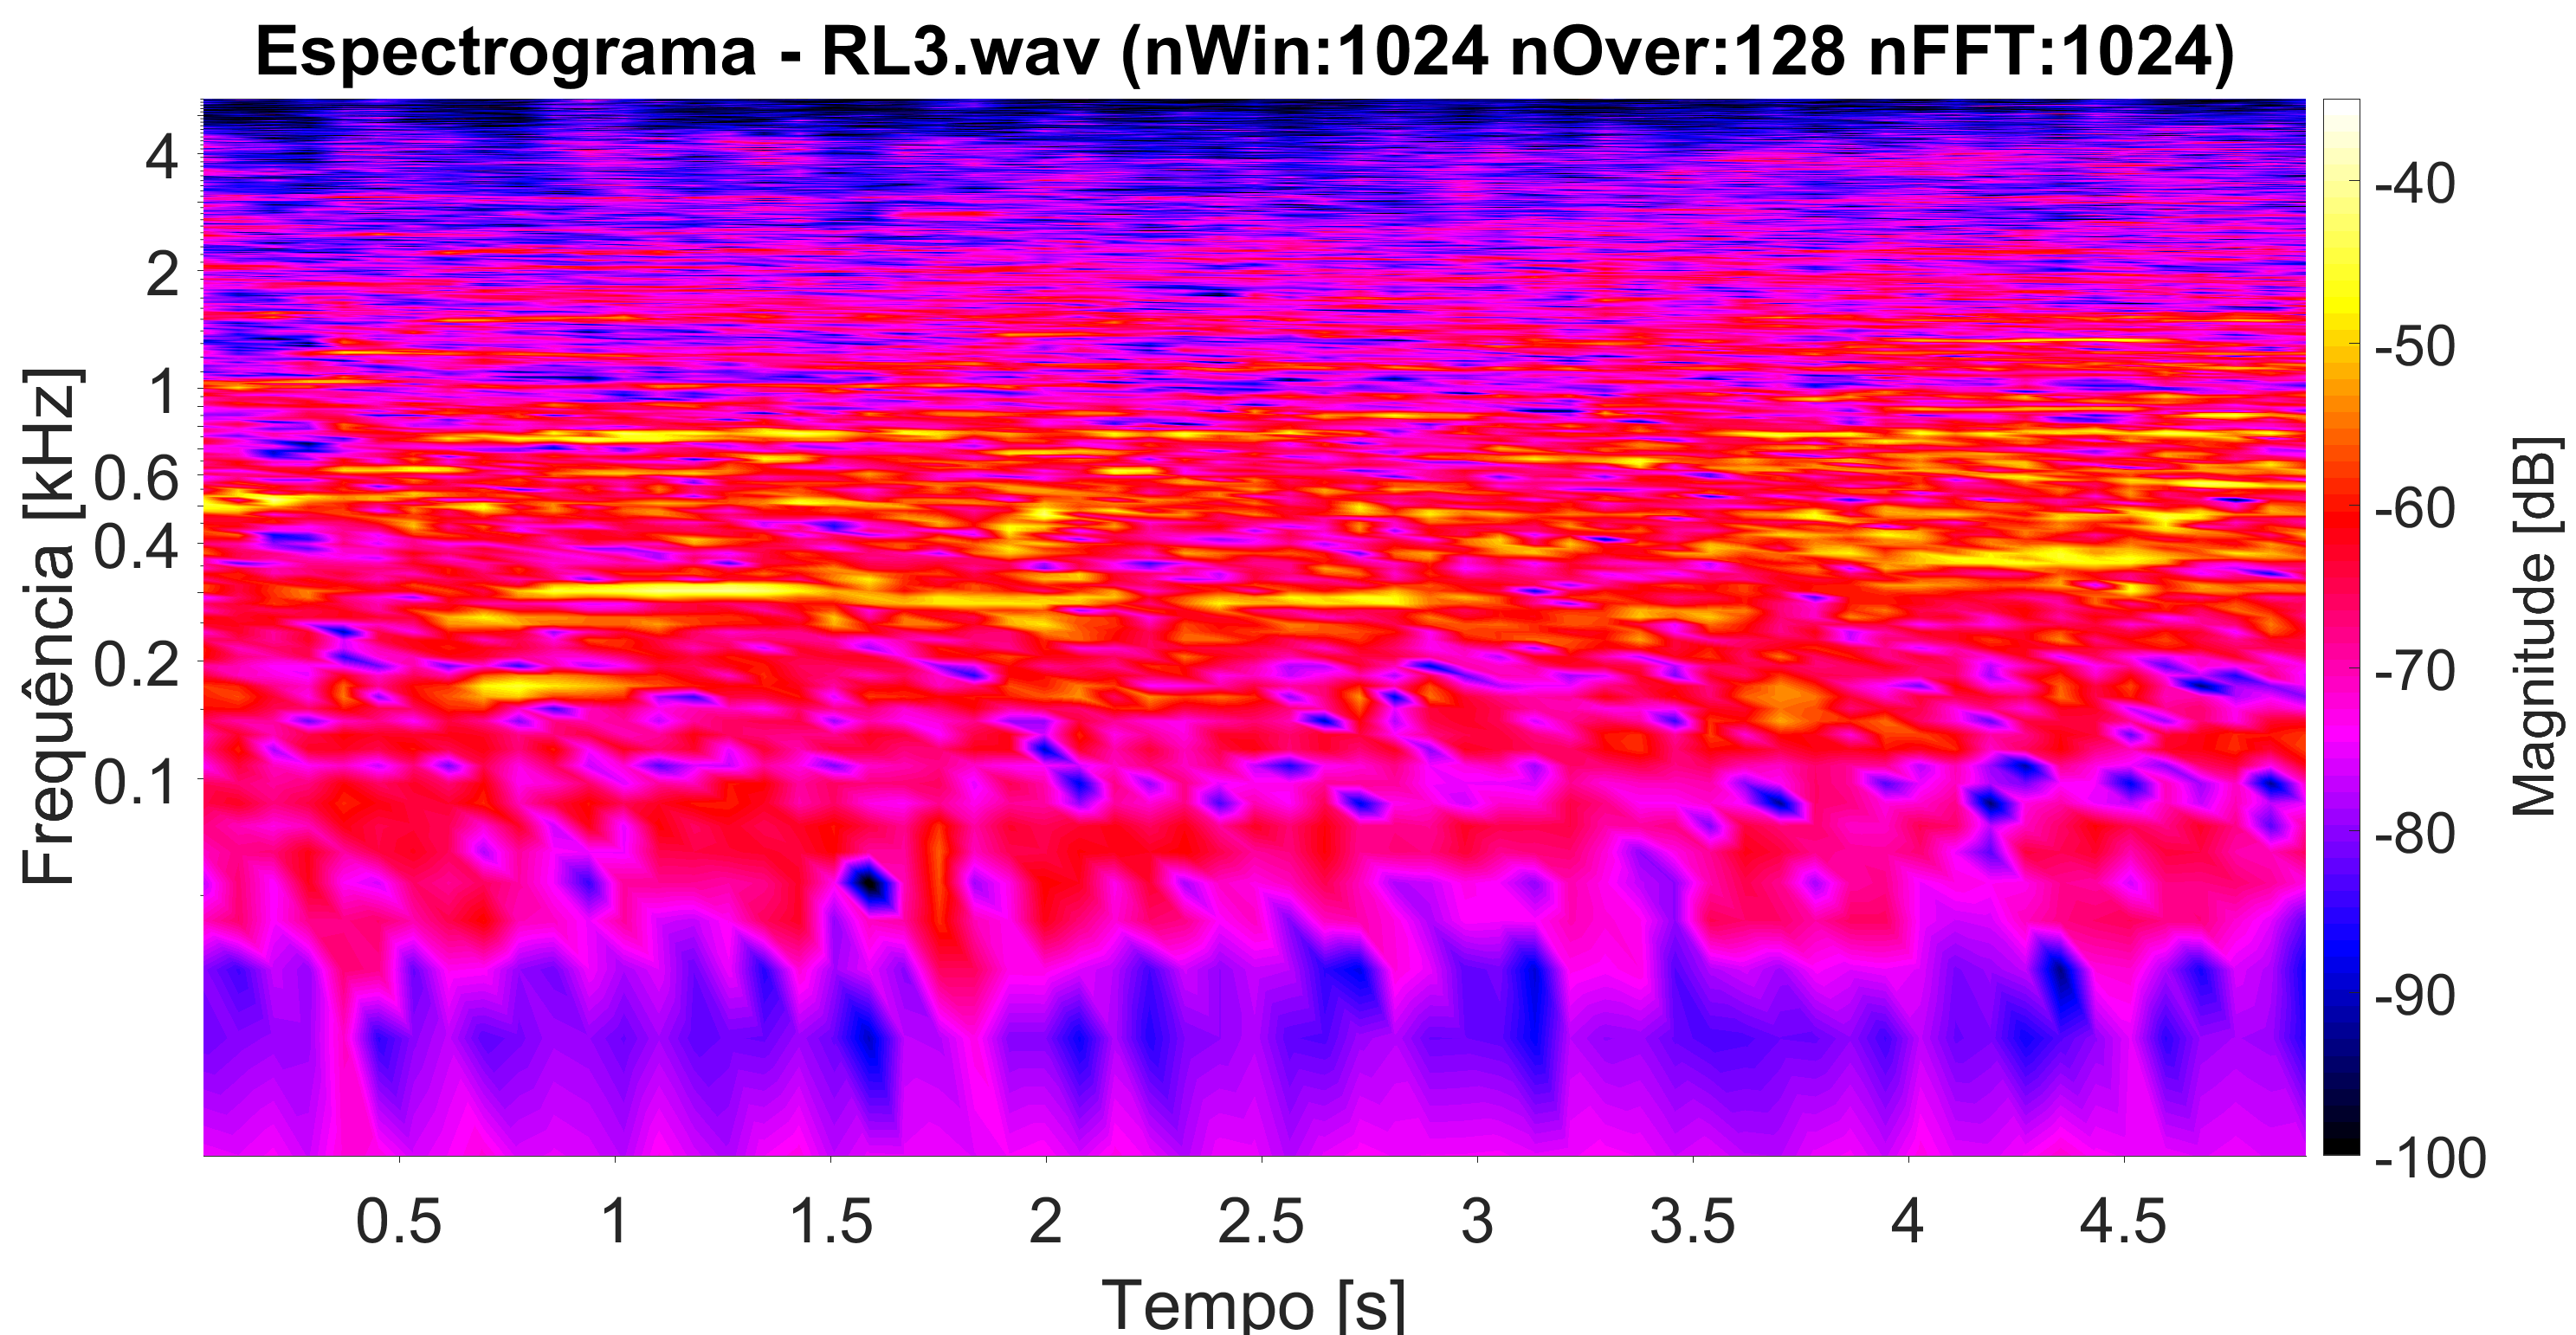
\includegraphics[width=8.5cm,]{Figs/RL3}}\quad \subfloat[asdasd]{\label{fRL4}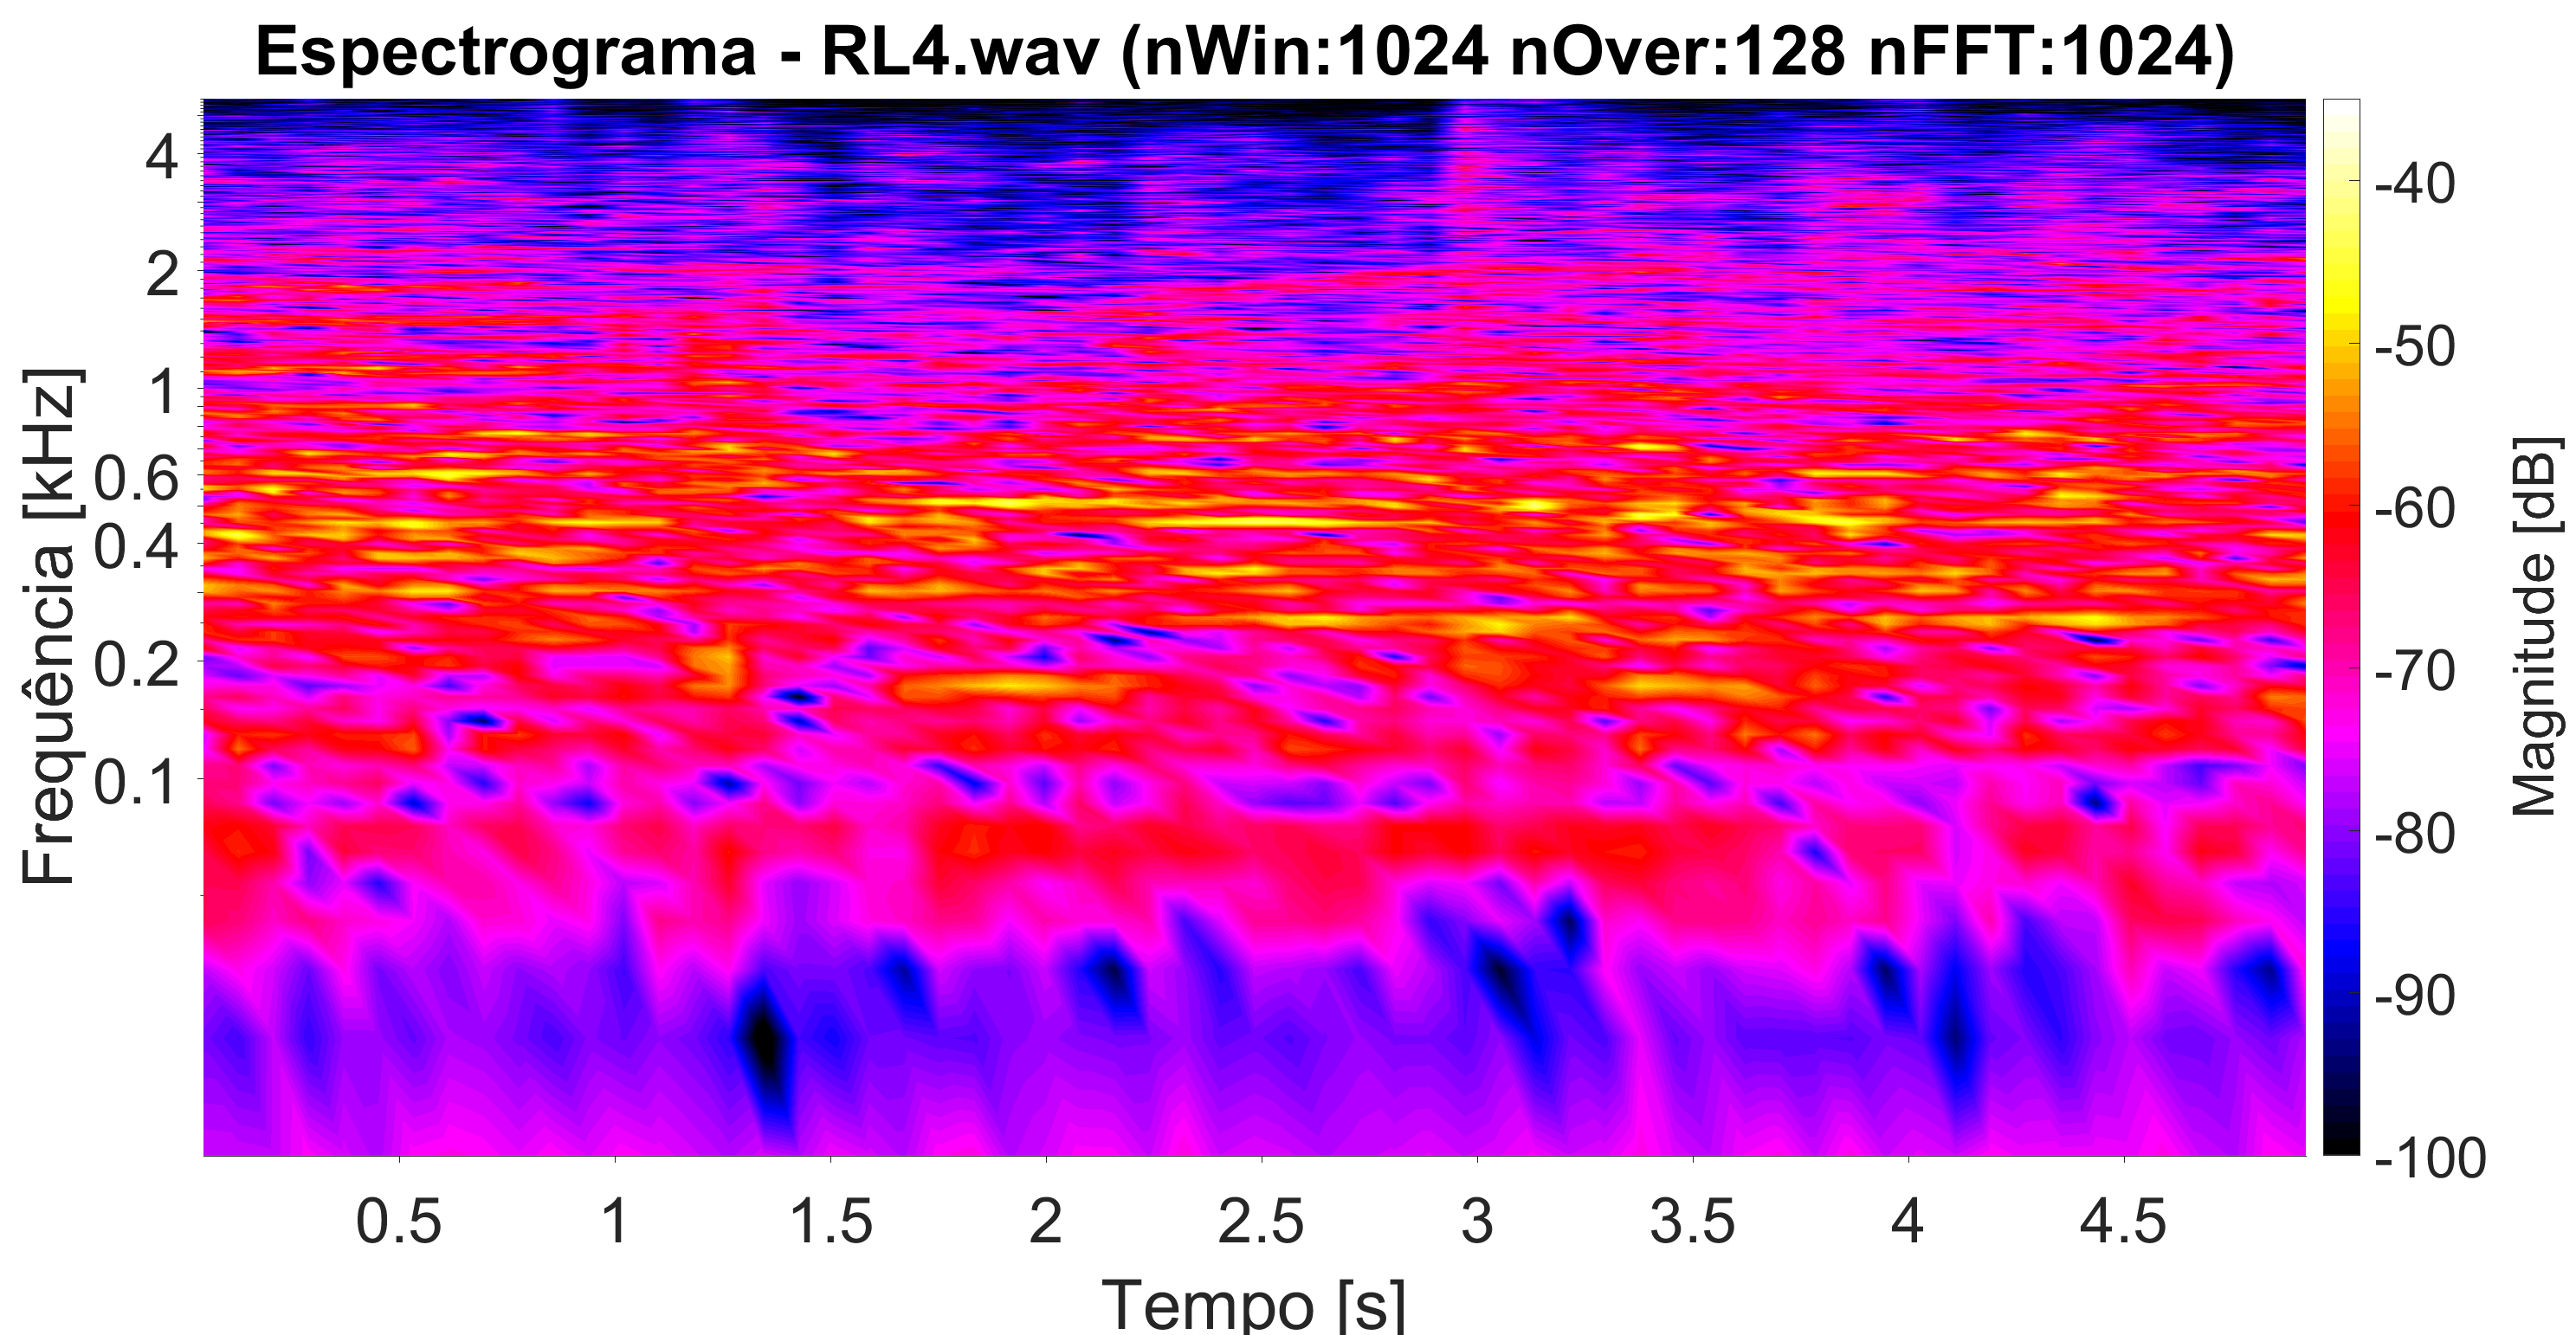
\includegraphics[width=8.5cm,]{Figs/RL4}}\\
 %  \subfloat[asdasd]{\label{fRL5}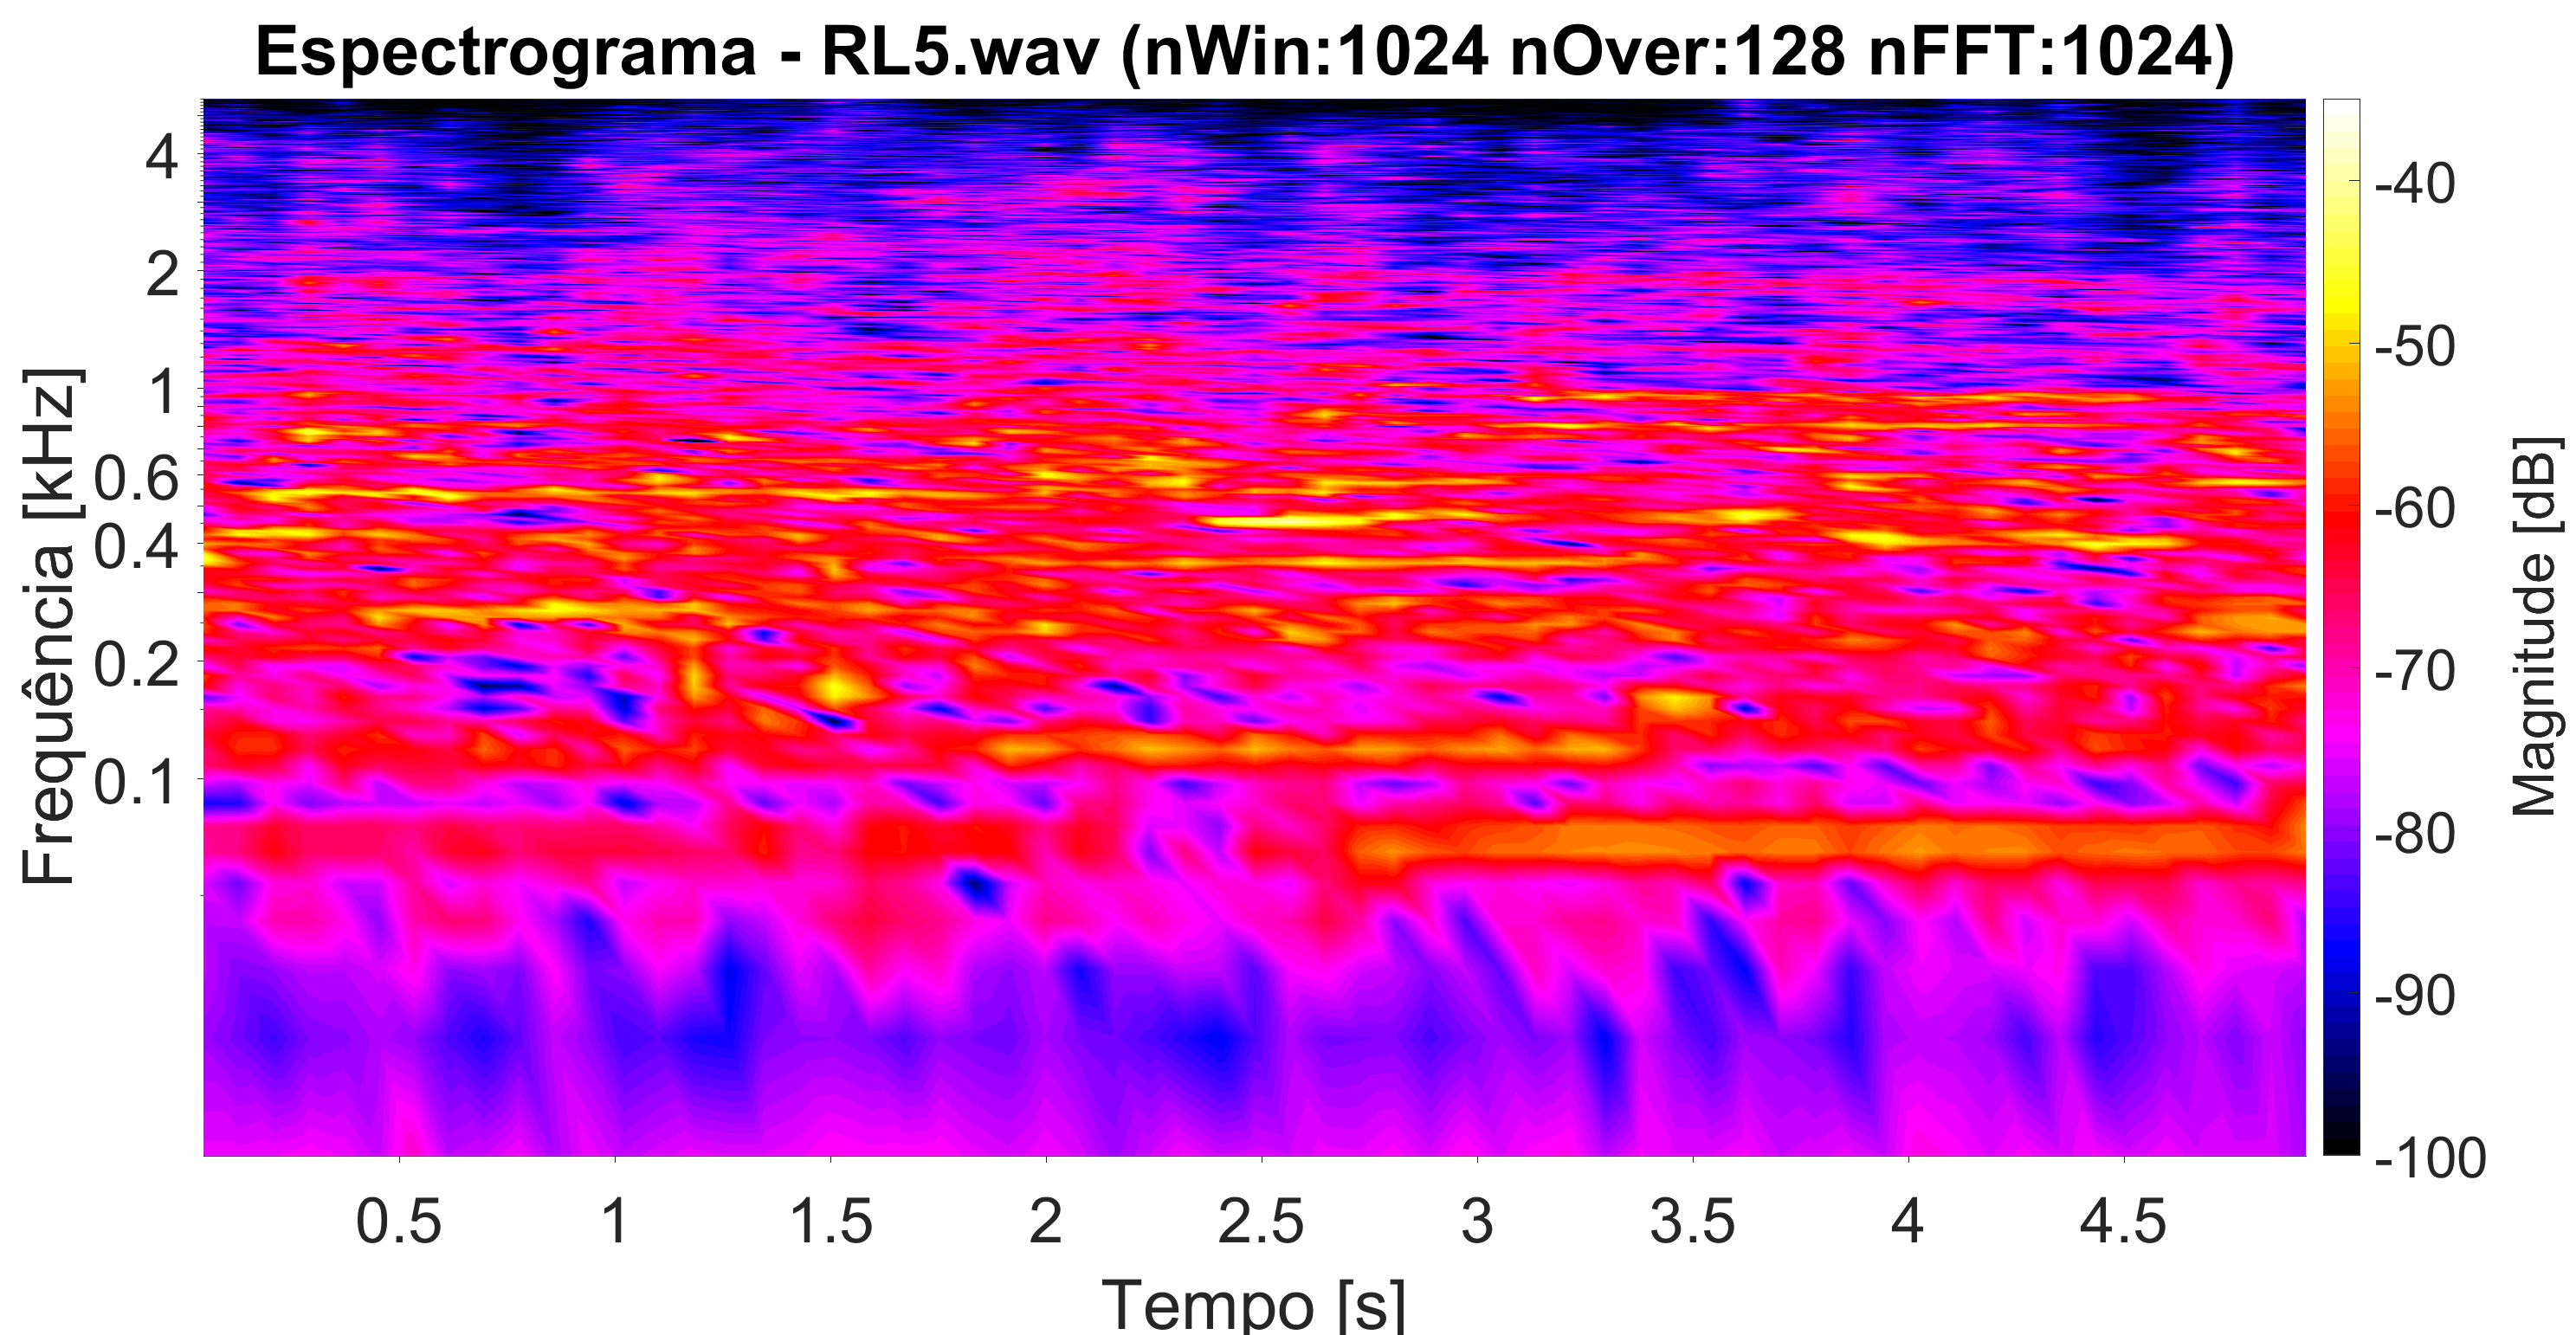
\includegraphics[width=8.5cm,]{Figs/RL5}\quad
%   \subfloat[SNR 10 dB.]{\label{fRL5}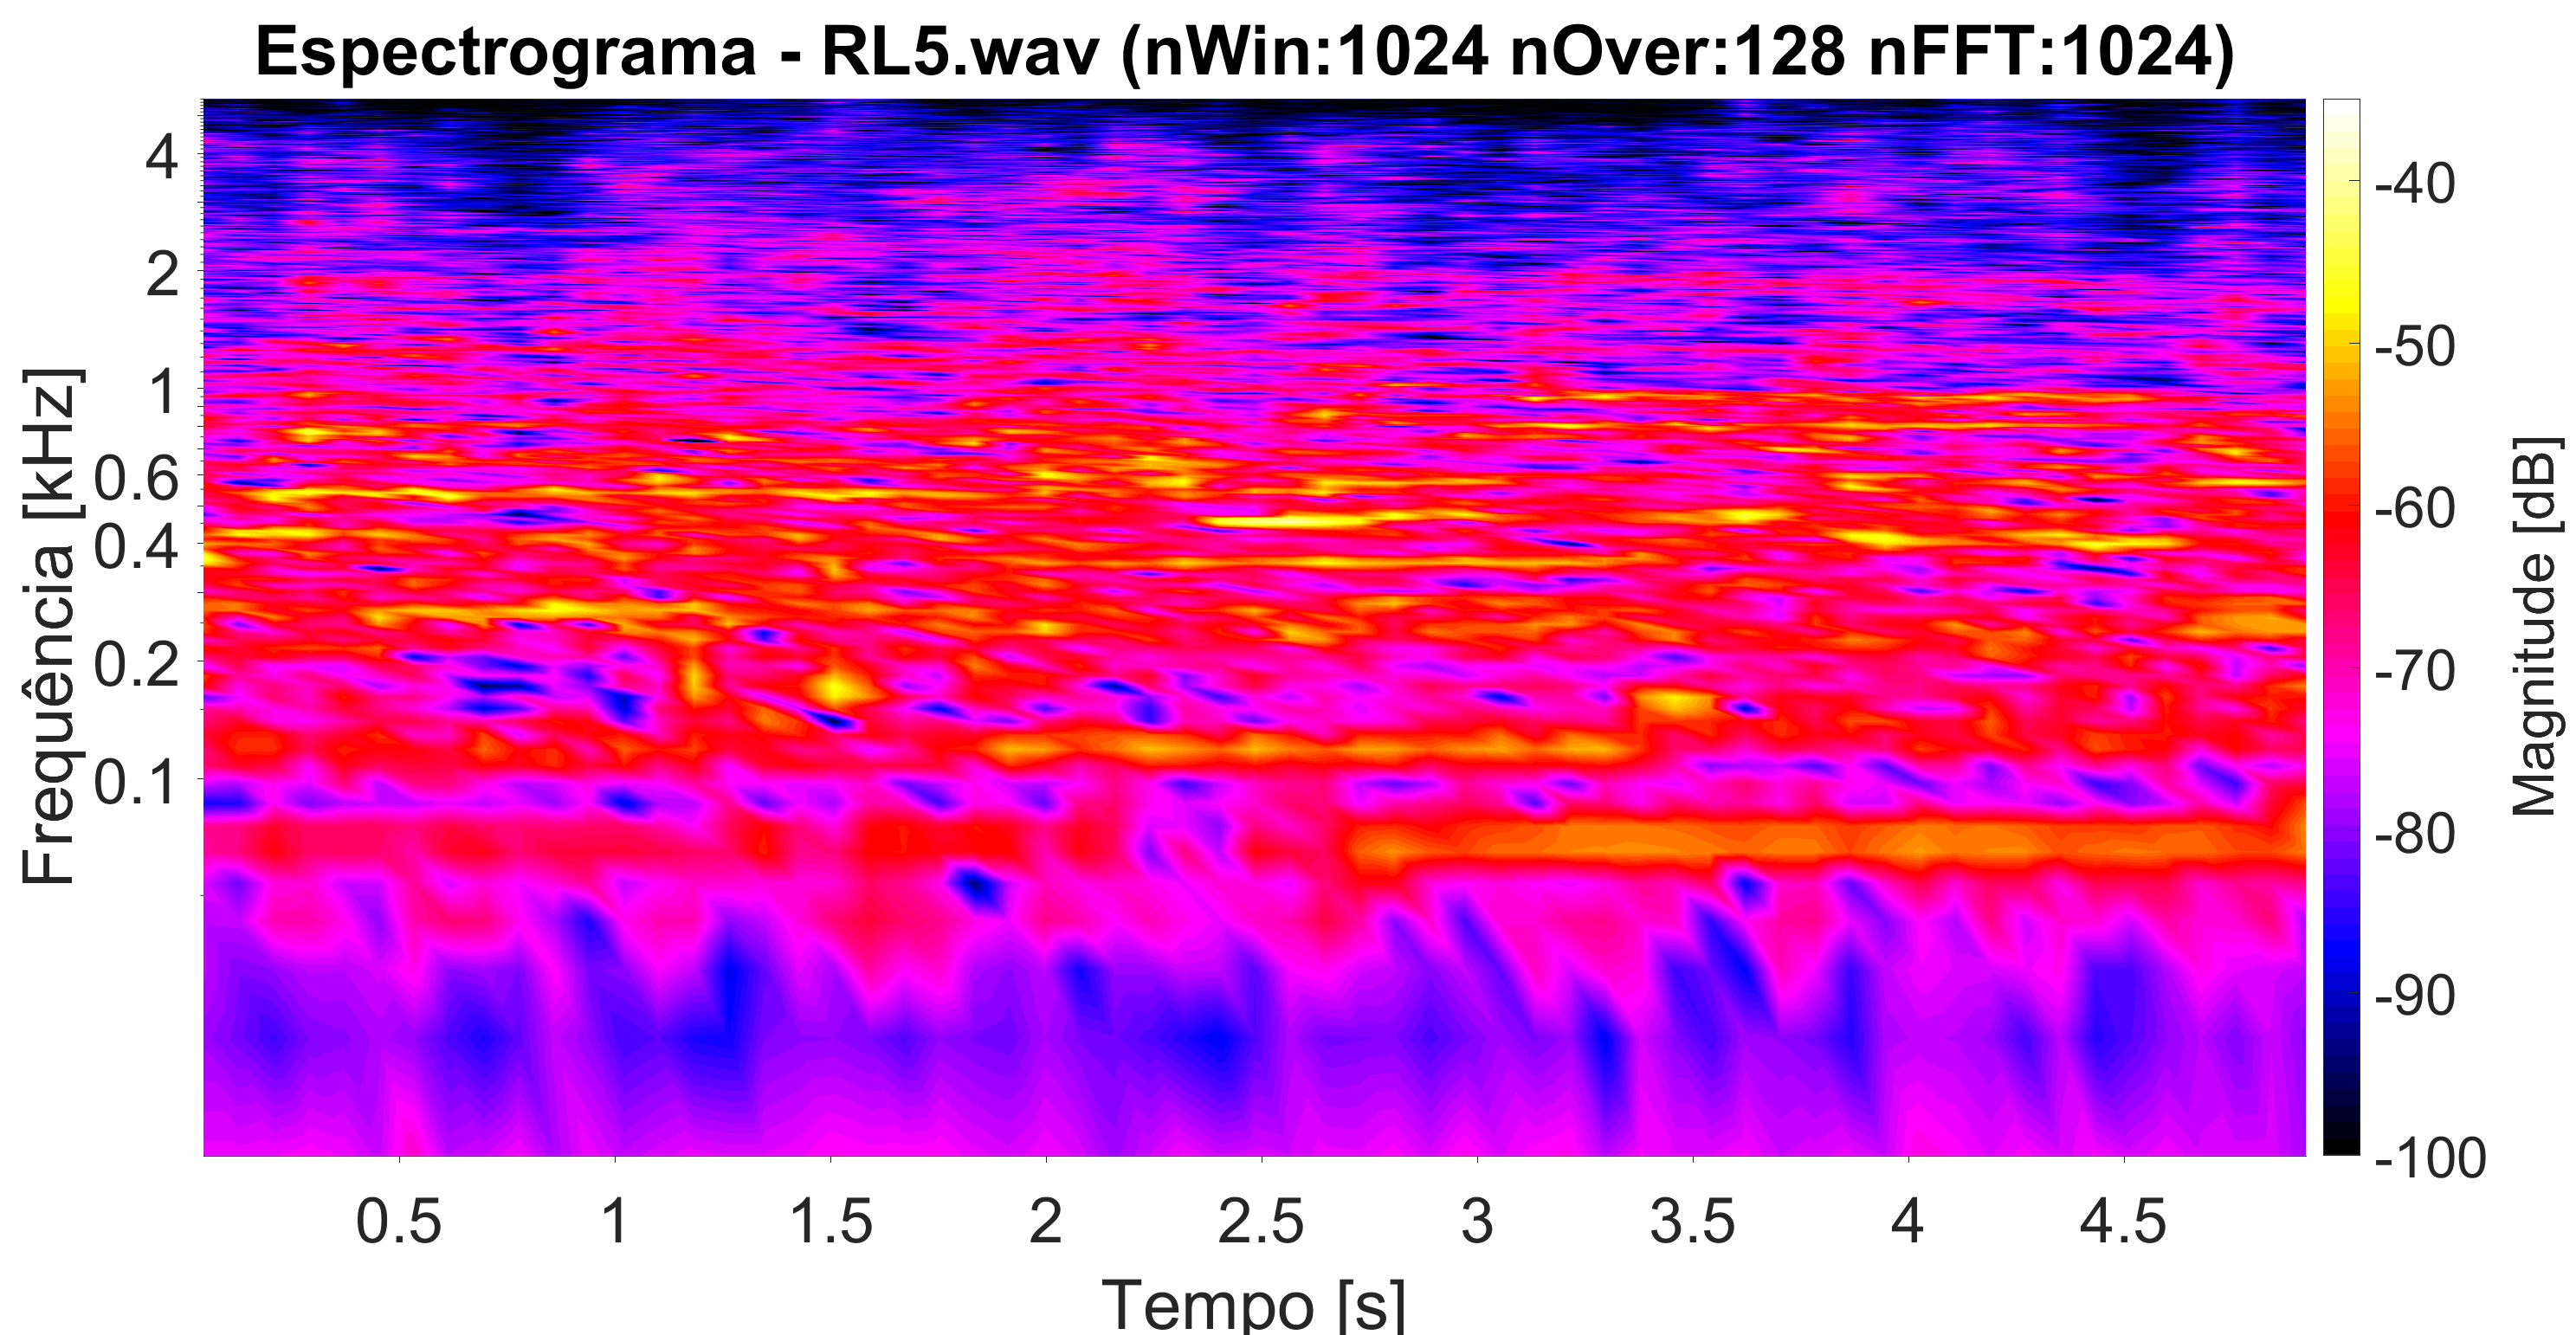
\includegraphics[width=8.5cm,]{Figs/RL5}\\
\caption{Espectrograma dos ruídos RL1 e RL2.}
\label{SRL}
\end{figure}

Do mesmo modo as \figuras{SRM} e \fign{SRMX} apresentam dois espectrogramas dos trechos de ruído cada.


\begin{figure}[H]
\subfloat[RM1]{\label{fRM1}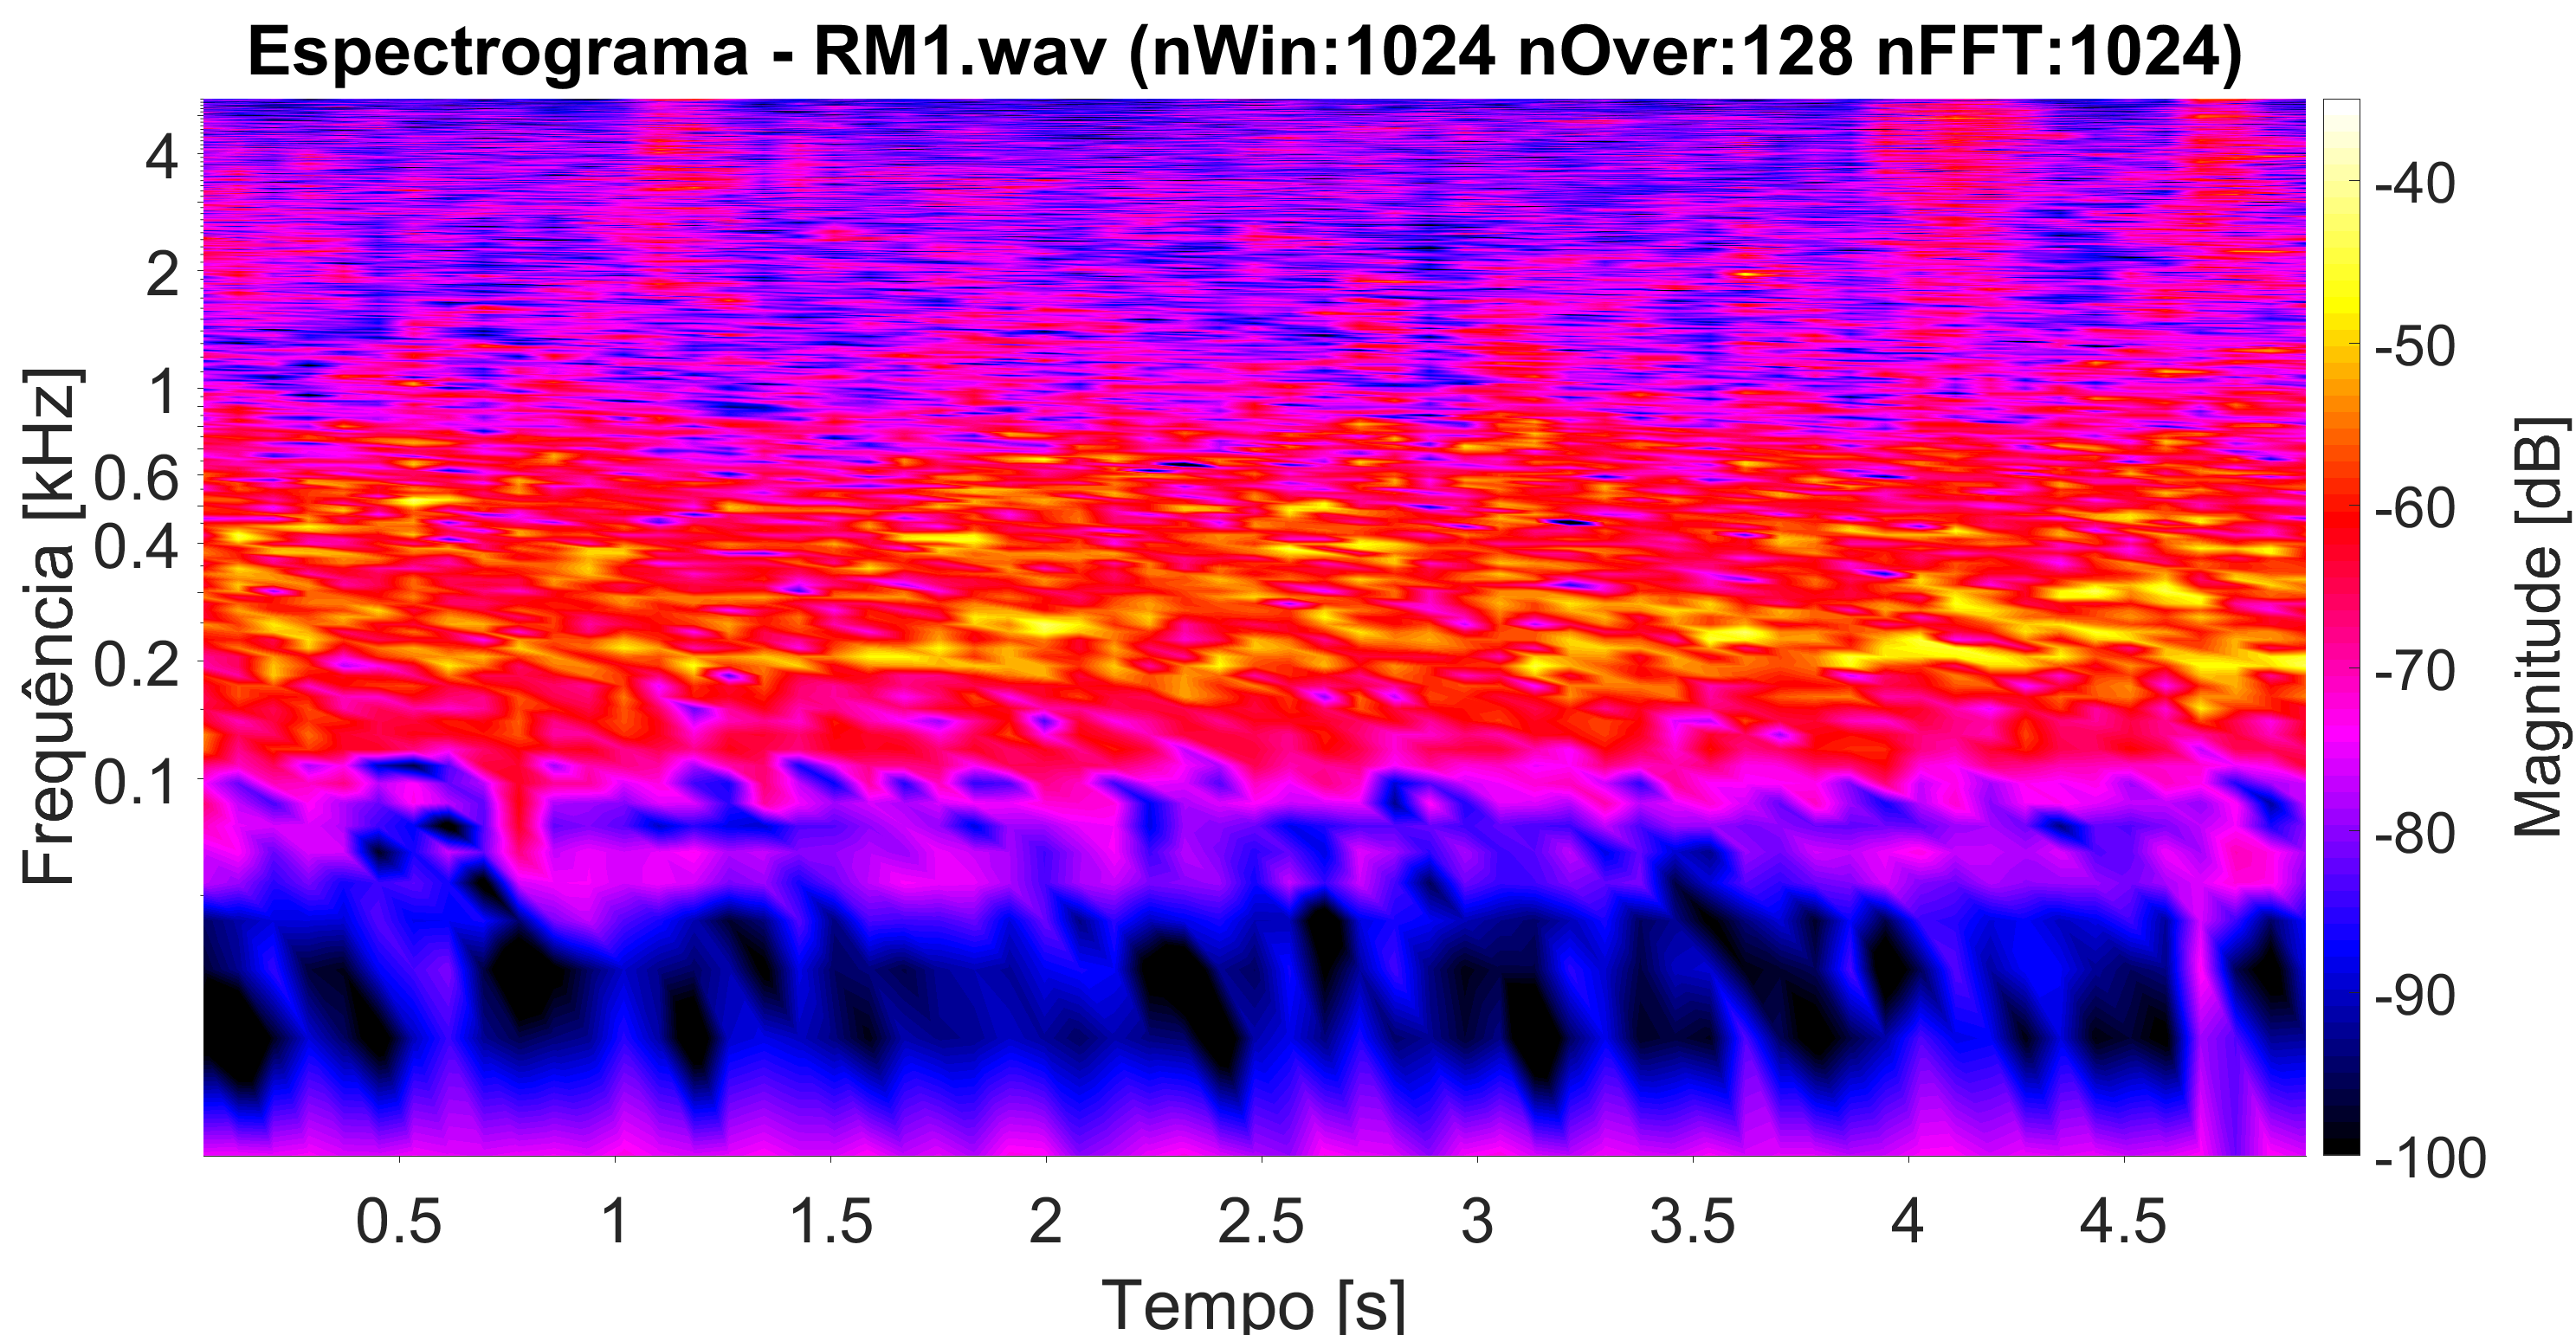
\includegraphics[width=8.5cm]{Figs/RM1}}\quad
 \subfloat[RM2]{\label{fRM2}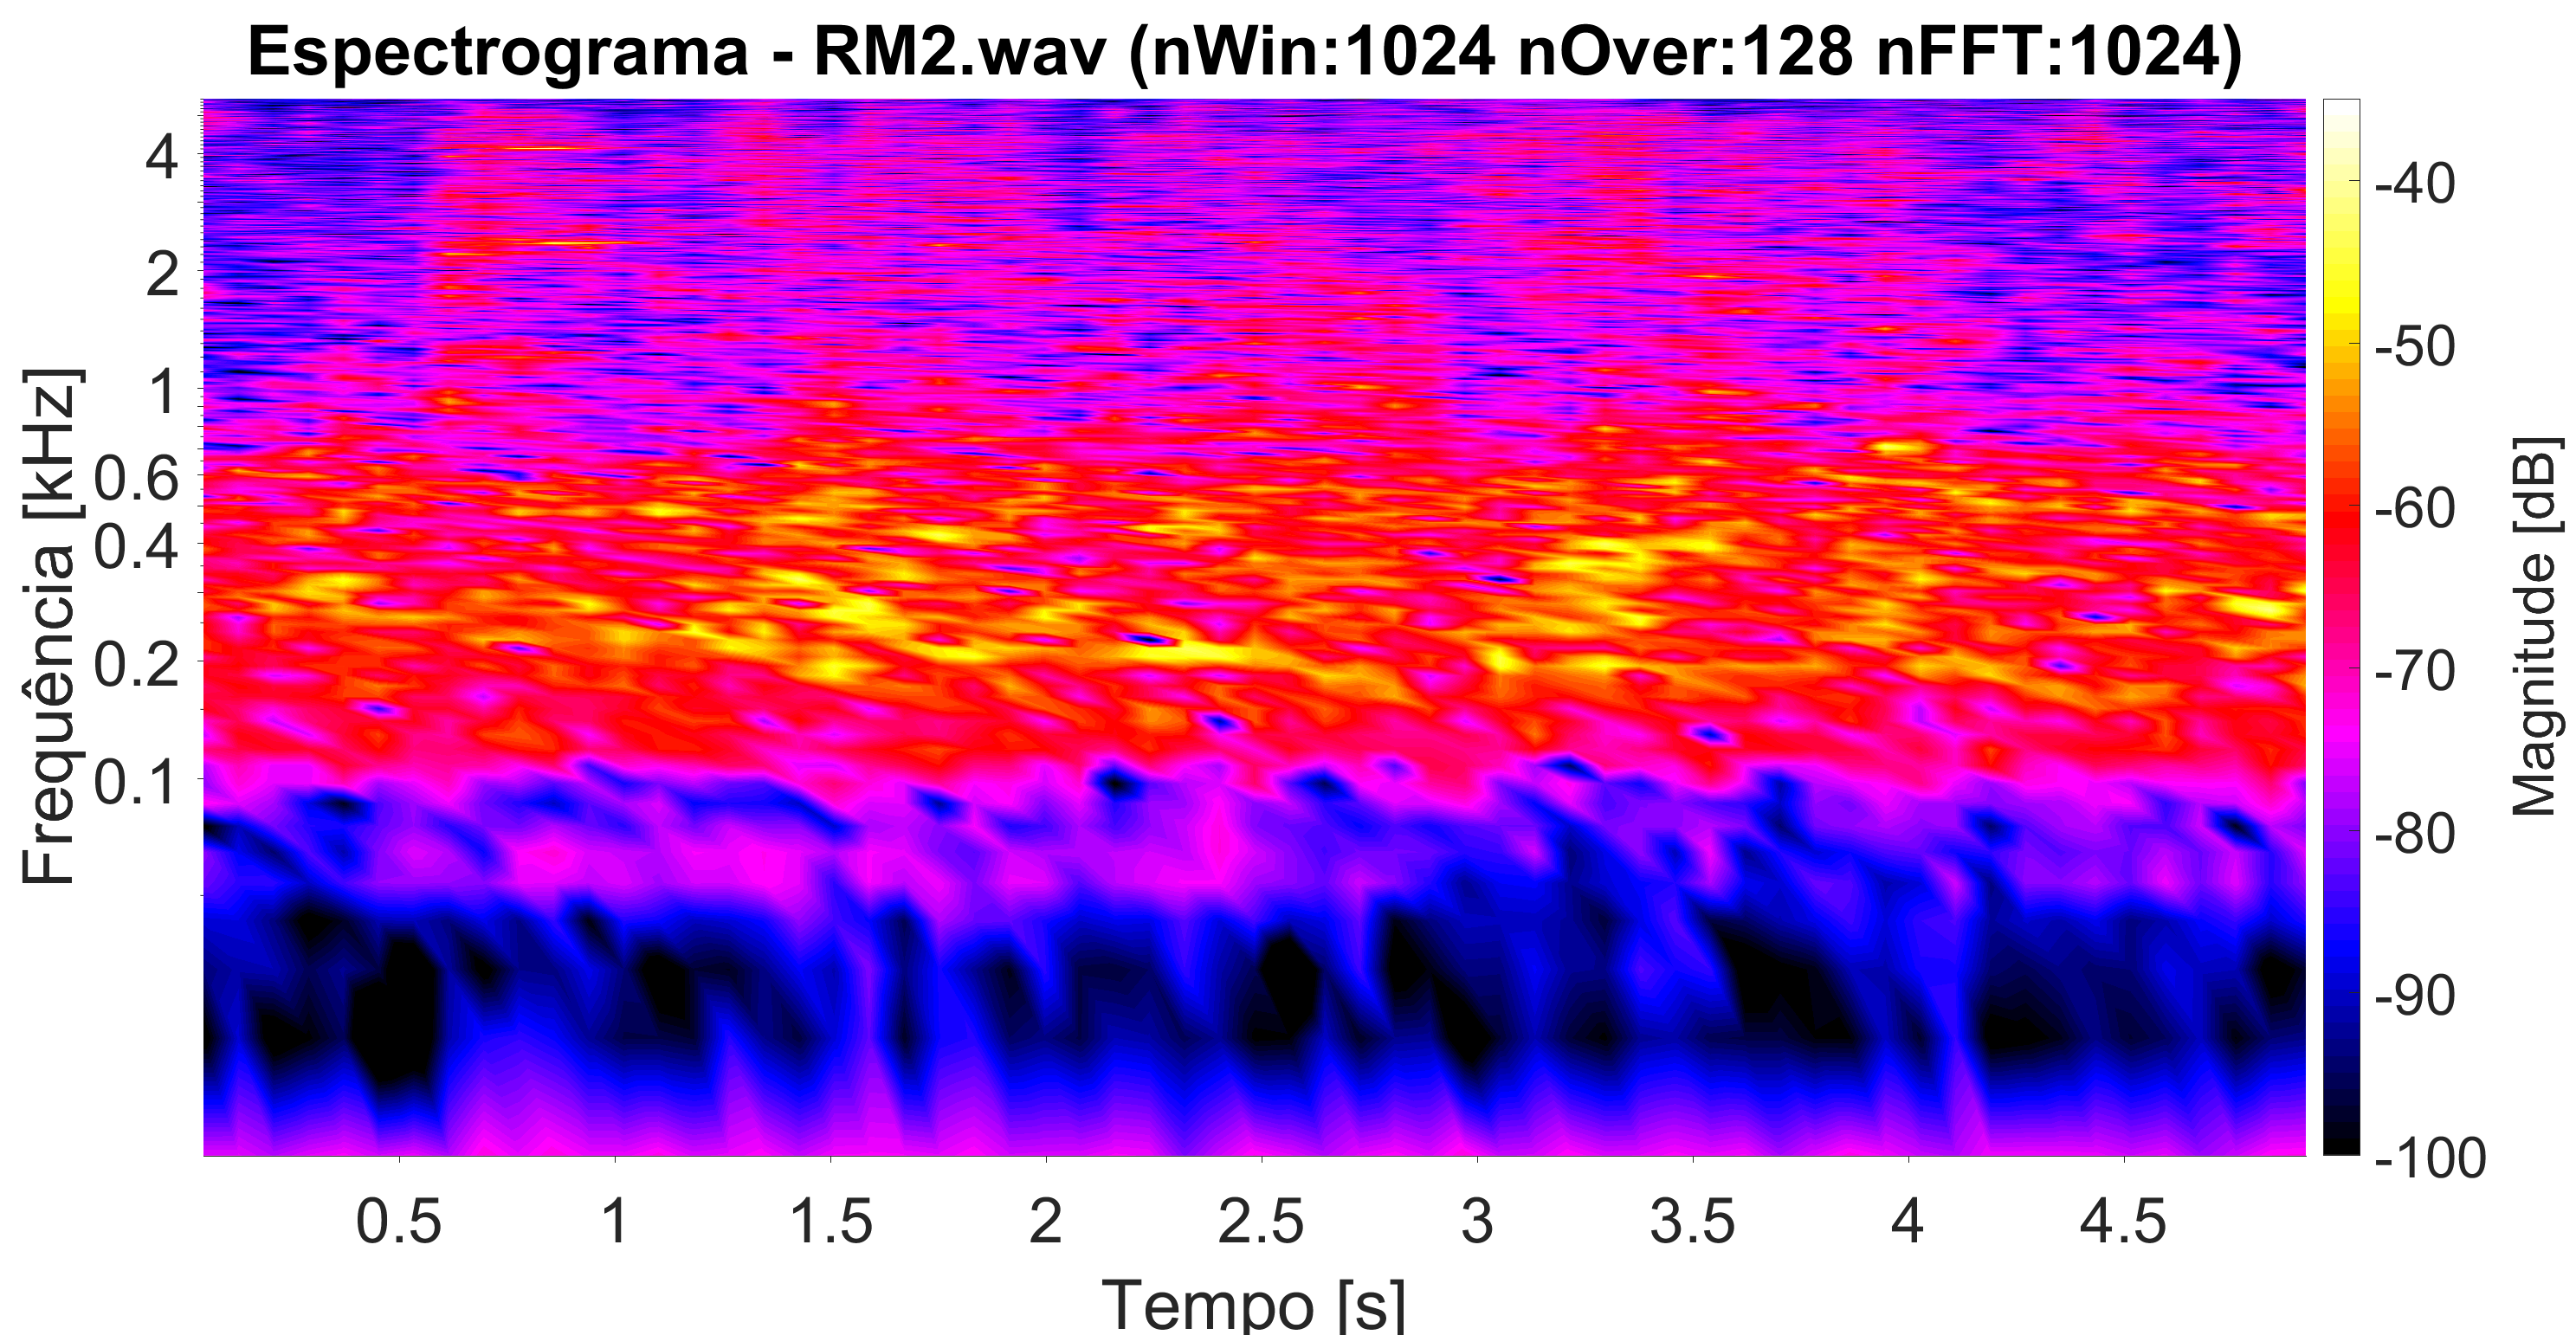
\includegraphics[width=8.5cm,]{Figs/RM2}}\caption{Espectrograma dos ruídos RM1 e RM2.}
\label{SRM}
\end{figure}

\begin{figure}[H]
\subfloat[RMX1]{\label{fRM1}\includegraphics[width=8.5cm]{Figs/RMX1}}\quad
 \subfloat[RMX2]{\label{fRM2}\includegraphics[width=8.5cm,]{Figs/RMX2}}\caption{Espectrograma dos ruídos RMX1 e RMX2.}
\label{SRMX}
\end{figure}

Considerando o espalhamento em frequência e a presença de música tocada ao violão o ruído RMX apresenta uma faixa de frequência limitada, aproximadamente entre aproximadamente 150~Hz e 1,5~kHz com picos abaixo dos 1~kHz. A contribuição do ruído aditivo RL apresenta a maior faixa de frequências, com magnitude consideráveis, entre os ruídos, ela apresenta sinais de baixa frequência (abaixo de 100~Hz) até aproximadamente 4~kHz, com picos entre 150~Hz e1k~Hz. o ruído RM não apresenta grandes magnitudes em baixas frequências, contudo extendendo-se até 4~kHz e com as maiores magnitudes apresentadas entre 200~Hz e 1~kHz.

Os Ruídos selecionados, ainda que tenham uma faixa de espectro variável, podem ser considerados como banda estreita, dado as maiores contribuições serem em uma faixa estreita. Contudo é importante frisar que essa faixa de frequência coincide com a faixa de frequência da fala, sendo que os ruídos, pelas características apresentadas (RMX: musical com fundo de \textit{babble noise}, RM: \textit{babble noise} e RL: \textit{babble noise} com fundo musical) tem grande relevância na inteligibilidade e qualidade da fala. 

\subsection{Qualidade}
O método escolhido para avaliação, na questão de aderência, quanto à qualidade da fala baseado na análise dos ruídos foi o PESQ de banda estreita (350-3.250~Hz). Para a diversidade de comparação o método da medida de distância espectral de Itakura Saito foi escolhido. 

\subsubsection{PESQ}

O método de avaliação \textit{Perceptual Evaluation of Speech Quality} (PESQ) é um modelo de predição de respostas subjetivas da voz de banda estreita. A filtragem, a variação de atraso e ou distorção e a degradação (inicialmente desenvolvido para avaliação de sistemas telefônicos) são os fatores de relevância para o método. A partir da combinação do modelo psicoacústico do PSQM+ e do alinhamento temporal do \textit{Perceptual Analysis Measurement System} (PAMS) o modelo tenta prever a resposta subjetiva à qualidade sonora \cite{simao2007}. 

O PESQ é um método intrusivo (necessita do áudio/sinal original) que compara o sinal original com o sinal degradado, com a predição da resposta subjetiva apresentada na escala tipo (MOS) \textit{Mean Opinion Score}~\cite{loizou2013speech}, sendo essa resposta que seria apresentada dada a apresentação do sinal degradado a um conjunto de sujeitos.

Os sinais são alinhados no tempo e podem ser aplicados em banda estreita (PESQ) ou banda larga (PESQ \textit{Wideband}) e transformados do domínio do tempo e magnitude amplitude, para o domínio da frequência com a magnitude representada em \textit{Loudness}. Assim a subtração entre os espectros (agora de \textit{loudness}, representam as diferenças audíveis acumuladas ao longo do tempo e ponderadas de de acordo com a distorção ou segmentação do sinal final. A partir dessa análise é gerada a pontuação em uma escala onde 1 representa baixa qualidade e 5 representa qualidade excelente \cite{simao2007}.

O diagrama de blocos do PESQ é apresentado na \figura{fpesq}

\begin{figure}[H]
\centering
\includegraphics[width=8.5cm]{Figs/PESQ}
\caption[Diagrama de blocos do método PESQ de avaliação objetiva.]{Diagrama de blocos do método PESQ de avaliação objetiva \cite{loizou2013speech}.}
\label{fpesq}
\end{figure}

O método aplica o modelo de Zwicker para o \textit{loudness}, sendo

\begin{equation}
S(b) = S_i \left(\dfrac{P_0(b)}{0,5}\right)^{\gamma} \cdot \left[ \left(0,5 + 0,5 \cdot \dfrac{B'_x(b)}{P_0(b)}\right)^{\gamma} -1\right]..
\end{equation}
\noindent
Onde
$S_i$ é o fator de escala de \textit{loudness}\\
$P_0$ é o limiar absoluto para a banda crítica b (escala Bark)\\
$B'_x(b)$ [e a compensação em frequência do espectro em escala Bark\\
e $\gamma$ é 0,23 para $b \geq 4$ e ligeiramente maior se $b < 4$

A degradação $r_n(b)$ é avaliada na frequência através dos espectros de \textit{loudness} como
\begin{equation}
r_n(b) = S_n(b)-\bar{S_n}(b)
\end{equation}
\noindent
Sendo 
$S_n(b)$ a magnitude do espectro em \textit{loudness} do sinal original da banda crítica\\
$S_n-\bar{S_n}(b)$ a magnitude do espectro em \textit{loudness} do sinal corrompido da banda crítica

O efeito de mascaramento $m_n(b)$ em frequência (causado pelo formato da onda de flexão e da largura de banda referente a população de neurônios excitados maior em baixa frequência) é considerado a partir da \equacao{masc}

\begin{equation}
m_n(b) = 0,25\cdot\text{min}{S_n(b),\bar{S_n}(b)}
\label{masc}
\end{equation}

A partir do mascaramento a densidade de degradação $D_n(b)$ é calculada. No passo seguinte, a partir do fator de assimetria $AF_n(b)$ é calculado o fator de degradação assimétrica $DA_n(B)$

$$DA_n(b) = AF_n(b)\cdot D_n(b) \ \ \,\,\, 1\leq b\leq 42 $$

No estágio final o PESQ avalia a degradação com uma média no tempo com dois intervalos diferentes de duração e duas diferentes normalizações. Com uma média das ditorções a cada 320 milisegundos (20 frames) com 50\% de \textit{overlap} no janelamento retangular.

\begin{equation}
D_k'' = \left(\dfrac{1}{20}\sum\limits_{n=(k-1)20}^{20k-1}(D_n''^6)\right)^{\frac{1}{6}}
\end{equation}
\noindent
e 
\begin{equation}
DA_k'' = \left(\dfrac{1}{20}\sum\limits_{n=(k-1)20}^{20k-1}(DA_n''^6)\right)^{\frac{1}{6}} \,.
\end{equation}

Em seguida as médias da porção ativa da fala são normalizadas por um fator 2 de normalização.

\begin{equation}
d_{\text{sym}} = \left(\dfrac{\sum_k(D_k''t_k)^2}{\sum_k(t_k)^2}\right)^{1/2}
\end{equation}
e
\begin{equation}
d_{\text{asym}} = \left(\dfrac{\sum_k(DA_k''t_k)^2}{\sum_k(t_k)^2}\right)^{1/2}
\end{equation}
sendo
$t_k$ pesos aplicados ao frame degradado e depende do comprimento do sinal (sinais com menos de 1000 frames $t_k=1$).

O Valor obtido portanto é dado por:

\begin{equation}
\text{PESQ} = 4,5 - 0,1\cdot d_{\text{sym}} -0,0309\cdot d_\text{asym}
\end{equation}

A faixa de resultados é entre -0,5 e 4,5, contudo pode ser realizada com a escala MOS com valores entre 1 e 5.

\subsubsection{Itakura-Saito IS}
A distância de Itakura-Saito (também conhecida como medida de
distorção Itakura-Saito) foi desenvolvida em 1970 por Fumitada Itakura and Shuzo Saito e é definida pela seguinte \equacao{eqis}~\cite{eduardo2009}.

\begin{equation}
d_{\text{IS}}(X(\omega),S(\omega)) = \dfrac{1}{2\pi} \int\limits_{-\pi}^\pi\left[\dfrac{S(\omega)}{X(\omega)}-\log\left(\dfrac{S(\omega)}{X(\omega)}\right)-1\right]\dt \omega
\label{eqis}
\end{equation}
\noindent
onde\\
$X(\omega)$ é o espectro do sinal\\ 
$S(\omega)$ é o espectro do sinal original. 

A distância de IS é sensível à amplitude dos sinais sob análise. A medida de degradação de IS entre a potência do espectro de cada \textit{bin} de frequência é dado por

\begin{equation}
d_{\text{IS}}(X_k^2,\hat{X}^2) = \dfrac{X_k^2}{X_k^k,\hat{X}^2} - \log\left( \dfrac{X_k^2}{X_k^k,\hat{X}^2}\right)-1
\end{equation}

A magnitude ao quadrado do estimador é dada por

\begin{equation}
\hat{X}^2 = \int_0^\infty=X_k^{k}p(X_k Y(\omega_k))\dt X_k
\end{equation}



Sendo que o erro de estimação positivo ($X_k - \hat{X_k} > 0$) sugere que a estimativa espectral é atenuada, já um erro negativo sugere uma amplificação da amplitude. Para evitar a atenuação dos segmentos de fala fracos (por exemplo, paragens, fricativas), o modelo modificado de IS $d_{\text{MIS}}$ considera uma penalização dos erros positivos mais fortemente do que os erros negativos~\equacao{dmiss}

\begin{equation}
d_{\text{MIS}}(X_k^2,\hat{X}^2) = \e^{((X_k)-\hat{X_k})}-(X_k-\hat{X_k})-1 \,.
\label{dmiss}
\end{equation}


Assim a medida de Itakura-Saito apresenta a não semelhança entre o sinal original e o sinal a ser analisado, tendo como característica do método o resultado de uma medida de semelhança entre dois vetores. No caso da fala é a medida de probabilidade de um vetor obtido de um sinal contaminado ou processado LPC (\textit{Linear predictive coding}) $b_k$ tenha sido computado a partir do sinal de fala original com coeficientes LPC $a_k$ \cite{leandro2007}.

\subsection{Inteligibilidade}
A inteligibilidade da fala é intrinsecamente relacionada com a qualidade, contudo a percepção de compreensão da fala é de extrema importância. Figuras de mérito que relacionem essa quantidade subjetiva de maneira objetiva podem, por exemplo, auxiliar no processo de recuperação da neuro-plasticidade em deficientes auditivos.

\subsubsection{Métrica \textit{Normalized-Covariance} (NCM)}
O NCM é baseado no \textit{speech transmission index} (STI) que é calculado a partir de uma razão de magnitudes entre as modulações de baixa frequência (AM relativo à fala) dos sinais recebido e enviado à uma sala. Assim o NCM utiliza o sinal limpo de voz como referência para determinar a inteligibilidade do sinal processado, ou seja, é um método intrusivo. Define-se a $\overline{SNR}_i$ da i-ésima banda como:
\begin{equation}
    \overline{SNR}_i = 10 \log{\bigg[\frac{r_i^2}{(1-r_i^2)}\bigg]},
\end{equation}
em que
\begin{equation}
    r_i = \frac{\sum\nolimits_{t} (x_i(t)-\mu_i)(y_i(t)-\nu)}{\sqrt{\sum\nolimits_{t} (x_i(t)-\mu_i)^2}\sqrt{\sum\nolimits_{t} (y_i(t)-\nu)^2}},
\end{equation}

\noindent
sendo:\\
$\mu_i$ e $\nu_i$ são os valores médios do sinal de fala limpa $x_i(t)$ e processado $Y_i(t)$, respectivamente, na banda $i$. 

O fator $r_i$ varia entre -1 e 1. Assim, pode-se determinar o parâmetro de \textit{transmission index} ($TI$), 
\begin{equation}
    TI_i = \frac{\overline{SNR}_i + 15}{30}, 
\end{equation}
\noindent
 fazendo uma média ponderada em cada banda de frequência (dando ênfase à fala, obviamente) com a função ponderação $W_i$, tem-se
\begin{equation}
    NCM = \frac{1}{\sum_{i=1}^{K} W_i}\sum_{i=1}^{K} W_iTI_i
\end{equation}

\subsubsection{\textit{Coherence based speech intelligibility index}}

A partir da consideração do espectro contaminado como $Y(\omega) = X(\omega)+N(\omega)$ onde $X(\omega)$ é o espectro complexo do sinal limpo e $N(\omega)$ o espectro complexo do ruído contaminante o Quadrado da Coerência de Magnitude \textit{magnitude-squared coherence}  (MSC) é definido por

\begin{equation}
    |\gamma_{XY}(\omega)|^2 = \dfrac{|P_{XY}(\omega)|^2}{P_{Xx}(\omega)P_{YY}(\omega)}
    \label{msceq}
\end{equation}
\noindent
Onde $P_{XY}(\omega) = EX(\omega)Y* (\omega)$ é a densidade espectral do espectro cruzado entre as densidades espectrais $P_{XY}(\omega)$ e $P_{YY}(\omega)$

O MSC foi incorporado na medida de avaliação de inteligibilidade da fala em efeitos de distorção  de aparelhos auditivos com ouvintes normais e deficientes auditivos, ao incluir essa medida denotou-se CSII, que é apresentada na \equacao{eqCSII}

\begin{equation}
    \text{CSII } = \dfrac{1}{M}\sum\limits_{m=0}^{M-1}\dfrac{\sum_j=1^kW(j)\cdot T_{\text{CSII}}(j,m)}{\sum_j=1^kW(j)} \,,
    \label{eqCSII}
\end{equation}
\noindent

Sendo $K$ o número de bandas contidas na largura de banda do sinal e $W(j)$ a função de importância da banda.

O termo $T_{\text{CSII}}(j,m)$ é um mapeamento linear da SNR$_\text{ESI}$ (que tem variação entre -15 e 15 dB) para uma escala entre 0 e 1. O SNR$_\text{ESI}$ é calculado pela \equacao{snresieq}

\begin{equation}
    \text{SNR}_\text{ESI}(j,m) = 10\cdot\log\dfrac{\sum_{k=1}^NG_j(\omega_k)\cdot\widehat{\text{MSC}}(\omega_k)\cdot|Y_m(\omega_k)|^2}{\sum_{k=1}^NG_j(\omega_k)\cdot\left[1-\widehat{\text{MSC}}(\omega_k)\right]\cdot|Y_m(\omega_k)|^2}
\end{equation}

\noindent
sendo  $G_j(\omega)$ o filtro ro-ex centrado na $j$-ésima banda crítica e $Y_m(\omega_k)$ o espectro do sinal sob avaliação no \textit{frame} $m$.\\

O $\widehat{\text{MSC}}(\omega)$ é a estimativa de MSC dado pela \equacao{msceeq}

\begin{equation}
\widehat{\text{MSC}}(\omega) = \dfrac{\left|\sum_{m=1}^MX_m(\omega)Y_m*(\omega)\right|^2}{\sum_{m=1}^M|X_m(\omega)|^2\cdot |\sum_{m=1}^MY_m(\omega)|^2}
    \label{msceeq}
\end{equation}


A medida CSII acima referida é calculada utilizando todos os \textit{frames} M do enunciado colocando ênfase igual em todos os segmentos, incluindo vogais, consoantes e transições vogais/consoantes. Calculando separadamente a medida CSII para diferentes segmentos (isto é, vogais versus consoantes fracas) aumentou a correlação de CSII com escores de inteligibilidade\cite{loizou2013speech}.


\subsection{Resultados}
Nesta seção sáo apresentados os dados obtidos através do processamento dos sinais seguindo os mesmos critérios de entrada para os algoritmos, os mesmos sinais de fala do grupo geral e tendo assim:
\begin{itemize}
    \item 15 trechos de ruído
    \item 20 sinais de fala
    \item 5 relações sinal-ruído
    \item 4 técnicas diferentes de processamento
\end{itemize}

\subsubsection{Resultados de Qualidade}
\label{secqual}
As \figuras{q1} a \fign{q5} apresentam os resultados de estimativa de qualidade sonora a partir do erro médio quadrático entre as diferenças espectrais, utilizado no primeiro trabalho, a medida de diferença obtida pelo método Itakura-Saito e pelo método PESQ. 

Os gráficos do Erro médio quadrático e do método IS tem sua escala no eixo \textit{y} invertida, para melhor visualização, dado que quanto menor o erro, mais próximos seriam os espectros, e portanto a avaliação de qualidade, enquanto para o PESQ quanto maior a magnitude na escala MOS maior a qualidade. Assim, para análises qualitativas, a comparação dos gráficos é feita seguindo a maneira usual de quanto mais acima, melhor o valor da qualidade.

As \figuras{q1} e \fign{q2} apresentam as baixas relações sinal-ruído para as técnicas (-10e -5~dB), é possível notar, a primeira vista, que tanto a figura de Itakura-Saito quanto o erro médio quadrático apresentam magnitudes altas, ainda que com relação sinal ruido baixa. Para a filtragem de Wiener o erro médio quadrático não é sensível, enquanto para Itakura-Saito sim, dado o estimador Beyseano, com uma grande variação. Para o IS ainda mesmo os sinais sem processamento tiveram bom desempenho em todas SNR dado o método apresentar grande poder em relacionar por LPC \textit{Linear predictive coding} os coeficientes do sinal degradado aos coeficientes do sinal original (ferramenta importante no campo de \textit{speech recognition}). Ainda assim as medidas de qualidade a partir da diferença espectral apresentam valores altos por não levar em consideração fatores da psicoacústica da audição humana. Para o PESQ que toma em consideração tal fato, as magnitudes claramente são menores para todas as técnicas de subtração de ruído, enfocado na distorção apresenta baixos valores para os áudios sem processamento, tendo um aumento das magnitudes com o acréscimo da SNR. 
 

\begin{figure}[H]
\centering
\includegraphics[width=1\linewidth]{Figs/Total_m10}
\caption{Comparação entre os resultados obtidos pelos três métodos de estimação, o eixo x dos \textit{boxplot} refere-se a: 1-Logmmse, 2-Wiener, 3-Logmmse SPU, 4-Subtração espectral, 5-Sem processamento.}
\label{q1}
\end{figure}

\begin{figure}[H]
\centering
\includegraphics[width=1\linewidth]{Figs/Total_m5}
\caption{Comparação entre os resultados obtidos pelos três métodos de estimação, o eixo x dos \textit{boxplot} refere-se a: 1-Logmmse, 2-Wiener, 3-Logmmse SPU, 4-Subtração espectral, 5-Sem processamento.}
\label{q2}
\end{figure}

A \figura{q3} apresenta a relação sinal-ruído de 0~dB de contaminação, há uma melhora na magnitude das técnicas utilizando o erro médio quadrático, e como anteriormente a técnica de subtração espectral apresentou melhor desempenho na mediana. Para a avaliação de IS praticamente não houve mudanças. Na avaliação PESQ é possível notar um ganho na magnitude mediana dos sinais processados por técnicas, contudo não do sinal sem processamento, o que é esperado. Para o PESQ nessa relação sinal-ruído a melhor técnica na mediana é a subtração espectral, com pouca diferença entre as técnicas.

\begin{figure}[H]
\centering
\includegraphics[width=1\linewidth]{Figs/Total_0}
\caption{Comparação entre os resultados obtidos pelos três métodos de estimação, o eixo x dos \textit{boxplot} refere-se a: 1-Logmmse, 2-Wiener, 3-Logmmse SPU, 4-Subtração espectral, 5-Sem processamento.}
\label{q3}
\end{figure}

As \figuras{q4} e \fign{q5} apresentam as altas relações sinal-ruído, ou seja, com menos contaminação, onde há um decréscimo na avaliação da filtragem Wiener pelo erro médio quadrático devido aos seus cortes em partes com silêncios, respirações e fricativos da fala. Para o IS também há um decréscimo, aparentemente pequeno para Wiener, as demais magnitudes mantêm-se alta ainda que com muitos \textit{outliers}, presentes também nas SNR anteriores, e também concentradas em magnitudes maiores. Para a avaliação PESQ é possível notar um aumento na mediana das técnicas em 5~dB e uma leve redução para 10~dB, mantendo-se a ordem da maior mediana para subtração espectral, seguido por Logmmse, Logmmse SPU e Wiener. A avaliação pelo PESQ apresenta o sinal contaminado com a menor mediana, ou seja, a menor avaliação de qualidade nessas relações sinal-ruído, contudo com \textit{outliers} consideráveis para magnitudes maiores.

\begin{figure}[H]
\centering
\includegraphics[width=1\linewidth]{Figs/Total_5}
\caption{Comparação entre os resultados obtidos pelos três métodos de estimação, o eixo x dos \textit{boxplot} refere-se a: 1-Logmmse, 2-Wiener, 3-Logmmse SPU, 4-Subtração espectral, 5-Sem processamento.}
\label{q4}
\end{figure}

\begin{figure}[H]
\centering
\includegraphics[width=1\linewidth]{Figs/Total_10}
\caption{Comparação entre os resultados obtidos pelos três métodos de estimação, o eixo x dos \textit{boxplot} refere-se a: 1-Logmmse, 2-Wiener, 3-Logmmse SPU, 4-Subtração espectral, 5-Sem processamento.}
\label{q5}
\end{figure}

\subsubsection{Resultados de Inteligibilidade}

As \figuras{i1} a \fign{i5} apresentam os resultados de estimativa de qualidade sonora a partir do erro médio quadrático entre as diferenças espectrais, utilizado no primeiro trabalho, a medida de coeficiente de correlação apresentada pelo método NCM e pelo método CSII. 

Para uma baixa relação sinal ruído (-10~dB e - 5~dB) (ver \figuras{i1} e \fign{i2}) a inteligibilidade do método Logmmse apresentou os melhores resultados nas figuras de mérito NCM e CSII, enquanto que utilizando erro médio quadrático ela apresentava o quarto melhor desempenho. A técnica de filtragem de Wiener apresenta boa representação ao utilizar-se o erro médio quadrático, enquanto com NCM e CSII ele apresenta um baixo nível de inteligibilidade. O Logmmse SPU apresenta comportamento semelhante ao obtido pelo Logmmse, contudo com menor magnitude da mediana em uma análise qualitativa. A subtração espectral apresentava a melhor mediana na métrica do erro médio quadrático, nas outras métricas apresenta um comportamento de mediana levemente melhor em comparação ao Logmmse SPU. O áudio não processado tem um grande espalhamento utilizando o erro médio quadrático, bem como nos demais, ainda aparece como uma magnitude bastante reduzida, indicando a dificuldade na inteligibilidade.

\begin{figure}[H]
\centering
\includegraphics[width=1\linewidth]{Figs/int_m10}
\caption{Comparação entre os resultados obtidos pelos três métodos de estimação, o eixo x dos \textit{boxplot} refere-se a: 1-Logmmse, 2-Wiener, 3-Logmmse SPU, 4-Subtração espectral, 5-Sem processamento.}
\label{i1}
\end{figure}


\begin{figure}[H]
\centering
\includegraphics[width=1\linewidth]{Figs/int_m5}
\caption{Comparação entre os resultados obtidos pelos três métodos de estimação, o eixo x dos \textit{boxplot} refere-se a: 1-Logmmse, 2-Wiener, 3-Logmmse SPU, 4-Subtração espectral, 5-Sem processamento.}
\label{i2}
\end{figure}

A partir da análise do desempenho dos métodos com as relações sinal-ruído anteriores, as proporções são mantidas entre as técnicas, contudo a magnitude cresce levemente, indicando uma melhora na inteligibilidade. \figura{i3}

\begin{figure}[H]
\centering
\includegraphics[width=1\linewidth]{Figs/int_0}
\caption{Comparação entre os resultados obtidos pelos três métodos de estimação, o eixo x dos \textit{boxplot} refere-se a: 1-Logmmse, 2-Wiener, 3-Logmmse SPU, 4-Subtração espectral, 5-Sem processamento.}
\label{i3}
\end{figure}

Nas condições de relação sinal ruído de 5dB e 10 dB as técnicas avançam na questão de inteligibilidade, contudo ao observar-se a filtragem de wiener, que tem um alto \textit{score} utilizando o erro médio quadrático, é drasticamente rebaixada nas figuras NCM e CSII, basicamente dado ao seu grande ataque no corte de informações. \figuras{i4} e \fign{i5}
\begin{figure}[H]
\centering
\includegraphics[width=1\linewidth]{Figs/int_5}
\caption{Comparação entre os resultados obtidos pelos três métodos de estimação, o eixo x dos \textit{boxplot} refere-se a: 1-Logmmse, 2-Wiener, 3-Logmmse SPU, 4-Subtração espectral, 5-Sem processamento.}
\label{i4}
\end{figure}

\begin{figure}[H]
\centering
\includegraphics[width=1\linewidth]{Figs/int_10}
\caption{Comparação entre os resultados obtidos pelos três métodos de estimação, o eixo x dos \textit{boxplot} refere-se a: 1-Logmmse, 2-Wiener, 3-Logmmse SPU, 4-Subtração espectral, 5-Sem processamento.}
\label{i5}
\end{figure}

\section{Avaliação Subjetiva}
A análise subjetiva solicitada no trabalho é para a qualidade sonora. Dado os resultados apresentados na seção~\ref{secqual} o teste proposto visa identificar as seguintes questões:

\begin{enumerate}
    \item A alta magnitude da avaliação da mediana sem processamento pelo IS nas diferentes SNR.
    \item Relação de qualidade sonora da filtragem Wiener para diferentes SNR entre as figuras de mérito.
    \item A relação entre erro médio quadrático, Itakura-Saito e PESQ para uma amostra de ruído em diferentes SNR.
    
\end{enumerate}

Para a parte \textbf{1} da avaliação subjetiva fora selecionado três sinais de áudio sem processamento, cada um proveniente de um ruído diferente, corrompidos com ruído nas SNR (-10, 0 e 10~dB). Os sinais são dispostos para o sujeito ouvi-los em ordem aleatória. Os 9 áudios recebem uma avaliação de 0 a 5 cada para a sua qualidade.

Para a parte \textbf{2} da avaliação são apresentados três sinais processados com a filtragem de Wiener nas SNR (-10, 0 e 10~dB) em comparação pareada ao sinal sem ruído e o avaliador dá uma nota de 0 a 5 para cada áudio processado em cada par avaliando a sua qualidade.

A parte \textbf{3} da avaliação propõe para o sujeito três sinais de ruído comparando nas SNR (-10, 0 e 10~dB) pelas 4 técnicas, cada um comparado com o sinal de referência corrompido com mesma SNR. Para esse teste o sujeito pode ouvir os áudios do par quantas vezes achar necessário e dá uma nota de 0 a 5 para o áudio avaliado. Para cada SNR são apresentados 4 sinais filtrados e o sinal não processado. 

Em todos os testes são adicionados 2 falsos testes, onde se compara a referência com a referência, ou apresentado o áudio sem processamento (caso parte 1 do teste)\footnote{Nesse caso se o sujeito avaliar o áudio sem ruído como menor valor de qualidade do que um áudio processado, é automaticamente invalidado}. Assim o será avaliada a confiabilidade intra-avaliador. A confiabilidade inter-avaliadores será analisada pela discrepância ou consonância dos dados.

\subsection{Resultados testes subjetivos}
Os resultados dos testes subjetivos são apresentados nesta seção. Os sujeitos avaliados não apresentaram queixas sobre a audição, utilizaram um fone Sennheiser HD 650, com o volume ajustável, sem treinamento prévio e conhecedores das técnicas e ruídos semelhantes, classificando-os como expecialistas.

\subsubsection{Parte 1}
A \tabela{t1s} apresenta o resultado da parte 1 do teste subjetivo com as notas para cada áudio.
% Please add the following required packages to your document preamble:
% \usepackage{graphicx}
\begin{table}[H]
\centering
\caption{My caption}
\label{t1s}
%\resizebox{\textwidth}{!}{%
\begin{tabular}{cccc}
\textbf{Parte 1} & \textbf{SNR - 10} & \textbf{SNR 0} & \textbf{SNR 10} \\
\textbf{Sinal 1 sujeito 1} & \textbf{2} & \textbf{4} & \textbf{5} \\
\textbf{Sinal 1 sujeito 2} & \textbf{2} & \textbf{4} & \textbf{4} \\
\textbf{Sinal 2 sujeito 1} & \textbf{1} & \textbf{3} & \textbf{4} \\
\textbf{Sinal 2 sujeito 2} & \textbf{2} & \textbf{3} & \textbf{4} \\
\textbf{Sinal 3 sujeito 1} & \textbf{3} & \textbf{4} & \textbf{5} \\
\textbf{Sinal 3 sujeito 2} & \textbf{2} & \textbf{4} & \textbf{5} \\
\textbf{Média} & \textbf{2} & \textbf{4} &\textbf{4,66}\\
\textbf{Sinal de referência sujeito 1} & \textbf{5} & \textbf{5} & \textbf{5} \\
\textbf{Sinal de referência sujeito 2} & \textbf{5} & \textbf{5} & \textbf{5}   
 
\end{tabular}%
% }
\end{table}


Para o caso a tendência é de aumento qualidade com o acréscimo de SNR em favor da fala, contudo com uma amostra maior poder-se-ia apresentar resultados quantitativos significativos, portanto o presente apresenta apenas a tendência, em conformidade com o esperado e confrontando a avliação objetiva que indicava altos valores para a qualidade em SNR baixas.

\subsubsection{Parte 2}

Os resultados do teste subjetivo aplicado aos dois sujeitos são apresentados na \tabela{tabnumero2}
\begin{table}[H]
\centering
\caption{Qualidade sonora com algoritmo de Wiener avaliada por sujeitos.}
\label{tabnumero2}
\begin{tabular}{cccc}
\textbf{\textbf{Parte 2}} & \textbf{SNR - 10} & \textbf{SNR 0} & \textbf{SNR 10} \\
\textbf{Sinal 1 suj 1 r1} & 0 & 1 & 4 \\
\textbf{Sinal 1 suj 2 r1} & 0 & 2 & 3 \\
\textbf{Sinal 1 suj 1 r2} & 0 & 2 & 4 \\
\textbf{Sinal 1 suj 2 r2} & 0 & 2 & 3 \\
\textbf{Sinal 1 suj 1 r3} & 0 & 1 & 4 \\
\textbf{Sinal 1 suj 2 r3} & 0 & 2 & 3 \\

\textbf{Sinal 2 suj 1 r1} & 0 & 1 & 2 \\
\textbf{Sinal 2 suj 2 r1} & 0 & 2 & 3 \\
\textbf{Sinal 2 suj 1 r2} & 0 & 1 & 4 \\
\textbf{Sinal 2 suj 2 r2} & 0 & 2 & 3 \\
\textbf{Sinal 2 suj 1 r3} & 0 & 1 & 4 \\
\textbf{Sinal 2 suj 2 r3} & 0 & 2 & 3 \\

\textbf{Sinal 3 suj 1 r1} & 0 & 1 & 4 \\
\textbf{Sinal 3 suj 2 r1} & 0 & 2 & 4 \\
\textbf{Sinal 3 suj 1 r2} & 0 & 1 & 4 \\
\textbf{Sinal 3 suj 2 r2} & 0 & 2 & 3 \\
\textbf{Sinal 3 suj 1 r3} & 0 & 1 & 4 \\
\textbf{Sinal 3 suj 2 r3} & 0 & 2 & 3 \\
\textbf{Média}  & \textbf{0,00} & \textbf{1,56} & \textbf{3,39}\\
\textbf{Mediana}  & \textbf{0,00} & \textbf{2,00} & \textbf{3,50}\\
% \textbf{Sinal ref sujeito 1} & 5 & 5 & 5 \\
% \textbf{Sinal ref sujeito 2} & 5 & 5 & 5 \\

\end{tabular}
\end{table}
A avaliação subjetiva apresenta uma tendência de correlação com as figuras de mérito objetivas. A comparação de forma qualitativa é apresentada na \figura{parte2} através das medianas. É importante notar que o eixo \textit{y} direito foi invertido, dado que uma menor magnitude apresenta uma maior correlação entre o sinal original e o processado, contudo para o erro médio quadrático da diferença espectral entre o sinal original e o sinal processado quanto maior a magnitude menor a correlação. Como a relação para o eixo \textit{y} esquerdo é positiva a mediana do erro médio quadrático apresenta também uma correlação (em escala relativa) condizente com o teste subjetivo. Apenas a medida de Itakura-Saito decresce em correlação dos sinais a partir de 0~dB o que pode ser influência da baixa amostragem de sinais, da diversidade de ruídos contaminantes ou de poucas avaliações subjetivas. 



\begin{figure}[H]
\centering
\includegraphics[width=1\linewidth]{Figs/parte2}
\caption{Comparação entre as medianas das figuras de mérito em questão e os resultados obtidos pelo teste subjetivo.}
\label{parte2}
\end{figure}

\subsection{Parte 3}
A terceira parte do teste visa apurar a relação entre erro médio quadrático, Itakura-Saito e PESQ para uma amostra de ruído em diferentes SNR na avaliação de qualidade sonora. Os resultados do teste são apresentados na \tabela{tab3}.
\begin{table}[H]
\centering
\caption{Comparação pareada entre audio processado por técnica e }
\label{tab3}
\begin{tabular}{cccc}
\textbf{Técnica/sujeito} & \textbf{SNR -10} & \textbf{SNR 0} & \textbf{SNR 10} \\
Wiener 1 sujeito        1 & 0 & 2 & 4 \\
Wiener 1 sujeito        2 & 0 & 3 & 4 \\
Wiener 2 sujeito        1 & 0 & 0 & 3 \\
Wiener 2 sujeito        2 & 0 & 3 & 4 \\
Wiener 3 sujeito        1 & 0 & 2 & 4 \\
Wiener 3 sujeito        2 & 0 & 3 & 3 \\
Logmmse 1 sujeito       1 & 0 & 4 & 4 \\
Logmmse 1 sujeito       2 & 0 & 3 & 4 \\
Logmmse 2 sujeito       1 & 0 & 2 & 4 \\
Logmmse 2 sujeito       2 & 0 & 4 & 5 \\
Logmmse 3 sujeito       1 & 0 & 4 & 4 \\
Logmmse 3 sujeito       2 & 0 & 4 & 5 \\
Logmmse SPU 1 sujeito   1 & 0 & 3 & 5 \\
Logmmse SPU 1 sujeito   2 & 0 & 4 & 5 \\
Logmmse SPU 2 sujeito   1 & 0 & 3 & 4 \\
Logmmse SPU 2 sujeito   2 & 0 & 3 & 5 \\
Logmmse SPU 3 sujeito   1 & 0 & 3 & 4 \\
Logmmse SPU 3 sujeito   2 & 0 & 3 & 5 \\
SpecSub 1 sujeito       1 & 0 & 1 & 4 \\
SpecSub 1 sujeito       2 & 0 & 2 & 3 \\
SpecSub 2 sujeito       1 & 0 & 1 & 3 \\
SpecSub 2 sujeito       2 & 0 & 2 & 3 \\
SpecSub 3 sujeito       1 & 0 & 2 & 5 \\
SpecSub 3 sujeito       2 & 0 & 2 & 4 \\
média & 0 & 2,62 & 4,10 \\
Sinal de referência sujeito 1 Wiener & 1 & 5 & 5 \\
Sinal de referência sujeito 2 Wiener & 1 & 5 & 5 \\
Sinal de referência sujeito 1 Logmmse & 1 & 5 & 5 \\
Sinal de referência sujeito 2 Logmmse & 2 & 5 & 5 \\
Sinal de referência sujeito 1 Logmmse SPU & 1 & 5 & 5 \\
Sinal de referência sujeito 2 Logmmse SPU & 2 & 5 & 5 \\
Sinal de referência sujeito 1 SpecSub & 1 & 5 & 5 \\
Sinal de referência sujeito 2 SpecSub & 1 & 5 & 5 \\

\end{tabular}
\end{table}

Para todas as técnicas o acréscimo da SNR gerou uma melhora na avaliação de qualidade, com uma amostra maior do teste subjetivo e a separação por ruídos no processamento dos dados, pode-se avaliar, futuramente, a efetividade para cada tipo dos ruídos, a partir de classificadores.

O trabalho deixa como propostas futuras a implementação de uma rodada experimental do grupo de controle com uma formulação de figura de mérito composta de diversas métricas e classificadores. Assim é possível determinar melhor os parâmetros de entrada e avaliar ainda melhor a relação entre resultados objetivos e subjetivos. Tendo isso é possível incluir nas rotinas de processamento classificadores para determinar a melhor técnica e os melhores parâmetros para este e futuros trabalhos.

\subsection{Protocolo de avaliação}
A disciplina contou com avaliações subjetivas dos alunos pela facilidade e comprometimento com a aula, contudo avaliações em seres humanos devem ser feitas respeitando o protocolo de pesquisa que é analisado pelo sistema CEP-CONEP. (Ver Anexo~\ref{anexo1}).

